\documentclass[english, 12pt, listof=totoc, tablecaptionabove, draft=true, twoside=true]{scrreprt}
% TODO: disable draft mode

\usepackage[a4paper, left=2.5cm, right=2cm, top=1.5cm, bottom=2cm, footskip=.8cm]{geometry}
\usepackage{scrhack}
% \usepackage[utf8]{inputenc}
\usepackage{babel}
\usepackage[table]{xcolor}
\usepackage[pdfborder={0 0 0}]{hyperref}
\usepackage[all]{hypcap}
\usepackage{amsmath}
\usepackage{graphicx}
\usepackage{float}
\usepackage{amsfonts}
\usepackage{textcomp}
\usepackage[titletoc]{appendix}

% REFERENCE: https://www.ctan.org/tex-archive/macros/latex/contrib/drawstack
% TODO: Install this package in the docker container / use offline version of it
\usepackage[nocolor]{drawstack}

\usepackage{lipsum}
% TODO: remove this in final builds

\usepackage[backend=biber,style=alphabetic,sorting=ynt]{biblatex}
\addbibresource{bibliography.bib}

\usepackage[T1]{fontenc}

\usepackage[no-math]{fontspec}
% \setmainfont{Times New Roman}
% \setsansfont{Arial}
\setmonofont[Scale=MatchLowercase]{JetBrains Mono NL}


\renewcommand{\labelitemii}{$\circ$}
\renewcommand{\labelitemiii}{$\vcenter{\hbox{\rule{.5ex}{.5ex}}}$}
\renewcommand{\labelitemiv}{$\vcenter{\hbox{\rule{.5ex}{.5ex}}}$}

% \setlength{\parindent}{0pt}
\setlength{\parskip}{4pt}

\usepackage[autostyle]{csquotes}

\newcommand{\TODO}[1]{\textcolor{red}{\textbf{TODO: #1}}}
\newcommand{\rushCommit}{\ignorespaces\texttt{\input "|git -C ./deps/rush rev-parse --short HEAD"}\unskip}
\newcommand{\paperCommit}{\ignorespaces\texttt{\input "|git rev-parse --short HEAD"}\unskip}
%\newcommand{\rushCountTests}{\ignorespaces{\input "|python3 ./deps/rush/samples/tests/main.py count-tests"}\unskip}
\newcommand{\rushCountTests}{\documentclass[english, 12pt, listof=totoc, tablecaptionabove, draft=true, twoside=true]{scrreprt}
% TODO: disable draft mode

\usepackage[a4paper, left=2.5cm, right=2cm, top=1.5cm, bottom=2cm, footskip=.8cm]{geometry}
\usepackage{scrhack}
% \usepackage[utf8]{inputenc}
\usepackage{babel}
\usepackage[table]{xcolor}
\usepackage[pdfborder={0 0 0}]{hyperref}
\usepackage[all]{hypcap}
\usepackage{amsmath}
\usepackage{graphicx}
\usepackage{float}
\usepackage{amsfonts}
\usepackage{textcomp}
\usepackage[titletoc]{appendix}

% REFERENCE: https://www.ctan.org/tex-archive/macros/latex/contrib/drawstack
% TODO: Install this package in the docker container / use offline version of it
\usepackage[nocolor]{drawstack}

\usepackage{lipsum}
% TODO: remove this in final builds

\usepackage[backend=biber,style=alphabetic,sorting=ynt]{biblatex}
\addbibresource{bibliography.bib}

\usepackage[T1]{fontenc}

\usepackage[no-math]{fontspec}
% \setmainfont{Times New Roman}
% \setsansfont{Arial}
\setmonofont[Scale=MatchLowercase]{JetBrains Mono NL}


\renewcommand{\labelitemii}{$\circ$}
\renewcommand{\labelitemiii}{$\vcenter{\hbox{\rule{.5ex}{.5ex}}}$}
\renewcommand{\labelitemiv}{$\vcenter{\hbox{\rule{.5ex}{.5ex}}}$}

% \setlength{\parindent}{0pt}
\setlength{\parskip}{4pt}

\usepackage[autostyle]{csquotes}

\newcommand{\TODO}[1]{\textcolor{red}{\textbf{TODO: #1}}}
\newcommand{\rushCommit}{\ignorespaces\texttt{\input "|git -C ./deps/rush rev-parse --short HEAD"}\unskip}
\newcommand{\paperCommit}{\ignorespaces\texttt{\input "|git rev-parse --short HEAD"}\unskip}
%\newcommand{\rushCountTests}{\ignorespaces{\input "|python3 ./deps/rush/samples/tests/main.py count-tests"}\unskip}
\newcommand{\rushCountTests}{\input{|python3 ./deps/rush/samples/tests/main.py count-tests}}
\newcommand{\qVerb}[1]{`\Verb{#1}'}
\newcommand{\riscv}{RISC\babelhyphen{nobreak}V}

% TODO: remove this command
\newcommand{\buildDate}{\ignorespaces\textcolor{red}{Timestamp: \texttt{\input "|date"} | Commit: \paperCommit}\unskip}

% \setcounter{tocdepth}{3}% Include \subsubsection in ToC

\usepackage{tabularx}
\usepackage{multirow}
\usepackage{makecell}
\renewcommand{\arraystretch}{1.2}
\newcolumntype{L}{X}
\newcolumntype{C}{>{\centering\arraybackslash}X}
\newcolumntype{R}{>{\raggedleft\arraybackslash}X}

\usepackage{keycommand}
\usepackage{fvextra}
\usepackage{float}
\usepackage{caption}
\usepackage[normalem]{ulem}

\captionsetup{margin=10pt, font=small, labelfont=bf, labelsep=endash}

\definecolor{hint}{HTML}{A0A1A7}
\fvset{
    breaklines=true,
    numbers=left,
    frame=lines,
    numbersep=12pt,
    rulecolor=\color{hint},
    framesep=2\fboxsep,
    fontsize=\footnotesize,
    labelposition=bottomline,
    % baselinestretch=1,
}
\renewcommand{\theFancyVerbLine}{\scriptsize\ttfamily\color{hint}\arabic{FancyVerbLine}}

\newfloat{listing}{htbp}{lol}[chapter]
\floatname{listing}{Listing}
% sets for all custom floats with `plain` style, but those are all listings in this document
\captionsetup[plain]{skip=0pt}

\newkeycommand+[°]{\TSListing}[
    first line,
    last line,
    caption,
    label,
    float,
    bool raw=false,
    bool raw queries=false,
][1]{
    % Default args
    °\def\args{%
        commandchars=×\{\},
    }°
    °\def\commandargs{}°
%
    % set `firstnumber` and `firstline` if `first line` is set
    \ifcommandkey{first line}{°\expandafter\def\expandafter\args\expandafter{\args%
        firstnumber=\commandkey{first line},
        firstline=\commandkey{first line},
    }°}{}
    % set `lastline` if `last line` is set
    \ifcommandkey{last line}{°\expandafter\def\expandafter\args\expandafter{\args%
        lastline=\commandkey{last line},
    }°}{}
    % set `label` if `caption` is set and `float` is unset
    \ifcommandkey{caption}{
        \ifcommandkey{float}{}{
            °\expandafter\def\expandafter\args\expandafter{\args%
                label=\textnormal{\color{black}\commandkey{caption}},
            }°
        }
    }{}
    \if\commandkey{raw}1°\expandafter\def\expandafter\commandargs\expandafter{\commandargs%
        --raw
    }°\fi
    \if\commandkey{raw queries}1°\expandafter\def\expandafter\commandargs\expandafter{\commandargs%
        --raw-queries
    }°\fi
%
    % begin float if `float` is set
    \ifcommandkey{float}{°\begin{listing}°[\commandkey{float}]}{}
    % actual input of code
    °\expandafter\VerbatimInput\expandafter[\args]°{|"ts2tex #1 °\commandargs°"}
    % end float and set caption and label if `float` is set
    \ifcommandkey{float}{
            \ifcommandkey{caption}{°\caption{\commandkey{caption}}°}{}
            \ifcommandkey{label}{°\label{\commandkey{label}}°}{}
        °\end{listing}°
    }{}
}

\newkeycommand+[°]{\AnsiListing}[
    first line,
    last line,
    caption,
    label,
    float,
][1]{
    % Default args
    °\def\args{%
        commandchars=×\{\},
        numbers=none,
    }°
    °\def\commandargs{}°
%
    % set `firstnumber` and `firstline` if `first line` is set
    \ifcommandkey{first line}{°\expandafter\def\expandafter\args\expandafter{\args%
        firstnumber=\commandkey{first line},
        firstline=\commandkey{first line},
    }°}{}
    % set `lastline` if `last line` is set
    \ifcommandkey{last line}{°\expandafter\def\expandafter\args\expandafter{\args%
        lastline=\commandkey{last line},
    }°}{}
    % set `label` if `caption` is set and `float` is unset
    \ifcommandkey{caption}{
        \ifcommandkey{float}{}{
            °\expandafter\def\expandafter\args\expandafter{\args%
                label=\textnormal{\color{black}\commandkey{caption}},
            }°
        }
    }{}
%
    % begin float if `float` is set
    \ifcommandkey{float}{°\begin{listing}°[\commandkey{float}]}{}
    % actual input of code
    °\expandafter\VerbatimInput\expandafter[\args]°{|"ansi2tex #1 °\commandargs°"}
    % end float and set caption and label if `float` is set
    \ifcommandkey{float}{
            \ifcommandkey{caption}{°\caption{\commandkey{caption}}°}{}
            \ifcommandkey{label}{°\label{\commandkey{label}}°}{}
        °\end{listing}°
    }{}
}

\usepackage{tikz}
\usetikzlibrary{shapes.geometric, shapes.multipart, fit, positioning}

\tikzstyle{rec} = [rectangle, minimum width=3cm, minimum height=1cm,text centered, draw=black]
\tikzstyle{arrow} = [thick,->,>=stealth]

% \tikzstyle{startstop} = [rectangle, rounded corners, minimum width=3cm, minimum height=1cm,text centered, draw=black, fill=_green!40]
% \tikzstyle{io} = [trapezium, trapezium left angle=70, trapezium right angle=110, minimum width=3cm, minimum height=1cm, text centered, draw=black, fill=blue!30]
% \tikzstyle{process} = [rectangle, minimum width=3cm, minimum height=1cm, text centered, draw=black, fill=orange!30]
% \tikzstyle{txt} = [minimum width=1cm, minimum height=1cm, text centered]
% \tikzstyle{decision} = [diamond, minimum width=3cm, minimum height=1cm, text centered, draw=black, fill=green!30]
% \tikzstyle{arrow} = [thick,->,>=stealth]

% \usepackage{pgfplots}

\pgfplotsset{compat=1.17}

% \plot[axis-options]{axis-environment}
\newcommand{\plot}[2][]{
    \begin{tikzpicture}
        \begin{axis}[
            grid=both,
            grid style=solid,
            axis equal,
            scale only axis,
            minor tick num=1,
            axis lines=middle,
            xlabel={x},
            ylabel={y},
            #1
        ]
            #2
        \end{axis}
    \end{tikzpicture}
}
% \addgraph[plot-options]{formula}
\newcommand{\addgraph}[2][]{
    \addplot[color=red, #1]
    {#2}
    ;
}
% \addpoint[plot-options]{coordinate}{pin-angle}{label}
\newcommand{\addpoint}[4][]{
    \addplot[
        color=black,
        mark=*,
        only marks,
        #1
    ]
    coordinates {(#2)}
    node[pin=#3:{#4}]{}
    ;
}
% \addsamples[plot-options]{coordinates}
\newcommand{\addsamples}[2][]{
    \addplot[color=blue, mark=*, #1]
    coordinates{#2}
    ;
}

% \usepackage{siunitx}

\newcommand{\m}{\SI{}{\metre}}
\newcommand{\km}{\SI{}{\kilometre}}
\newcommand{\cm}{\SI{}{\centimetre}}
\newcommand{\mm}{\SI{}{\millimetre}}
\newcommand{\dm}{\SI{}{\decimetre}}
\newcommand{\s}{\SI{}{\second}}
\newcommand{\minutes}{\SI{}{\minute}}
\newcommand{\h}{\SI{}{\hour}}
\newcommand{\ms}{\SI{}{\millisecond}}
\newcommand{\mpers}{\frac{\SI{}{\metre}}{\SI{}{\second}}}
\newcommand{\kmperh}{\frac{\SI{}{\kilometre}}{\SI{}{\hour}}}
\newcommand{\pers}{\SI{}{\per\second}}
\newcommand{\hz}{\SI{}{\hertz}}
\DeclareSIUnit{\microsecond}{\SIUnitSymbolMicro s}


\pagenumbering{gobble}

\titlehead{\centering
\includegraphics[width=7cm]{pictures/title.png}}
\title{The Conversion of Source Code to Machine Code}
\subtitle{Explaining the Basics of Compiler Construction Using a Self-Made Compiler}
\author{Silas Groh, Mik Müller}
\publishers{CFG Wuppertal}
\date{\today}

\begin{document}
\maketitle
\begin{abstract}
	\section*{Abstract}

    \buildDate

	Programming languages are undoubtedly of great importance for various aspects of
	modern-day life. Even if they remain unnoticed, digital systems running programs
	written in some sort of programming language are ubiquitous.
	However, there are numerous ways of implementing a programming language.
	A language designer could choose an interpreted or a compiled approach for their
	language's implementation. Both ways of program execution come with their own
	advantages and disadvantages.

	This paper aims to inform the reader about different means of program execution, focussing on compiler construction.
	However, we will only focus on the basics since implementing a programming language is often a demanding task.
	In order to include practical examples, we will explain concepts on the basis of our own programming language called \emph{rush}.
	During the implementation of rush, the focus for this paper has shifted slightly.
	As the title suggests, we originally planned on only implementing a compiler.
	However, there are numerous architectures which a compiler could target and settling on just one felt like the reader would miss out on too much.
	Therefore, we have implemented rush using one interpreter, one virtual machine, and five compilers.

	In chapter 1, we will give an introduction to implementing a programming language.
	Moreover, the rush programming language and its characteristics are presented.
	In chapter 2, the process of analyzing the program's syntax and semantics is explained.
	Chapter 3 focuses on how interpreters can be used in order to implement an interpreted programming language.
	Here, we will differentiate between a \emph{tree-walking interpreter} and a \emph{virtual machine}.
	The latter also serves as the target architecture for one of the five compilers.
	Chapter 4 illustrates how compilation to high-level\footnote{high-level targets: in this case machine independent} targets works.
	As examples for high-level targets, we will present the compiler targeting the virtual machine, a compiler targeting \emph{WebAssembly},
	and a compiler which uses the popular \emph{LLVM} framework.
	Chapter 5 focuses on how compilers targeting low-level\footnote{low-level targets: specific to one target architecture and operating system} architectures can be implemented.
    For this, we will present a compiler targeting \emph{\riscv{}} assembly and another compiler targeting \emph{x86\_64} assembly.
    Lastly, Chapter 6 presents final thoughts and a conclusion on the topic of implementing a programming language.
\end{abstract}

\tableofcontents

\cleardoublepage\pagenumbering{arabic}

\def\rushCommit{\ignorespaces\texttt{\input "|git -C ./deps/rush rev-parse --short HEAD | perl -pe 'chomp'"}\unskip}

\chapter{Introduction}
% This paper assumes that the reader has basic knowledge about computer programming and computer hardware.
% Most implementation code samples will be Rust code as the entire rush project is written in Rust.
Nowadays, computer programs are often written in formal, purposefully designed languages.
These languages introduce many constraints, such as syntactic and semantic rules, in order to allow
programmers to implement algorithms in a structured and precise manner.
Advantages of high-level languages are that program development is faster and easier, that programs are easier to maintain, and that programs are portable,
meaning that the program can be executed on different architectures~\cite[p.~9]{Dandamudi2005Risc}.
Since programming languages should be easy to write for a human while being easy to understand by a computer,
they are often falsely regarded as mysterious.
The fundamental challenge is that a computer is only able to interpret a sequence of CPU instructions instead of a written program.
Therefore, the source program has to be translated into such a sequence of instructions before it can be executed by the computer.
Because programming languages are strictly defined by formal constraints, the translation process can be defined formally as well.
Therefore, this translation can be automated and implemented as an algorithm on its own.
This process is referred to as \emph{compilation}, and is usually performed by a program called a \emph{compiler}.
It is apparent that compilation requires significant effort and must obey complex rules
since it should translate the source program precisely without altering its meaning.

Another common method of program execution is to implement a program, often referred to as an \emph{interpreter}, which interprets the source code directly.
Although compilers and interpreters share some of their core principles, their major difference is that the interpreter omits translation.
The implementation of an interpreter is often significantly easier and smaller since the interpreter only has to understand the source program in order to execute it.
In other words, the step of translating the source program into another form can be avoided completely.
However, implementing an interpreter is only sensible if it is written using a high-level language like C or Rust.
Implementation of an interpreter in a high-level language is often favorable since the implementation language is able to save the programmer a lot of work.
If an interpreter was to be implemented using a low-level language like assembly, there would not be much work done by the implementation language.
Compared to interpreters, compilers played an essential role in the early days of computing as high-level languages were yet to be developed.

The first compiler was implemented around 1956 and aimed to translate \emph{Fortran} to computer instructions.
However, the success of this programming endeavor was not assured until the program was completed.
In total, the poject involved roughly 18 man-years of work
and is thereby regarded as one of the largest programming projects of the time.
To this day, new compilers are created and innovations in the field of programming languages can be observed regularly.
Therefore, compiler construction can still be considered a fundamental and relevant topic in computer science~\cite[p.~6]{wirth_compiler_construction_2005}.

\section{Stages of Compilation}\label{sec:stages_of_compilation}
In order to minimize intricacy and to maximize modularity, compilation often involves several individual steps.
Here, the output of step $s$ serves as the input for step $s + 1$.
However, partitioning the compiler into as many steps as possible is prone to cause inefficiencies during compilation.
Separating the process of compilation into individual steps was the predominant technique until about 1980.
Due to limited memory of the computers at the time, a single-step compiler could not be implemented.
Therefore, only the individual steps of the compiler would fit,
as each step occupied a considerate amount of machine memory.
These types of compilers are called \emph{multi-pass compilers}.
However, the output of each step would be serialized and written to disk, ready to be read by the next step.
It is obvious that this partitioning leads to a lot of performance overhead, since disk access if often significantly slower than memory access.
Nowadays, we can mitigate these performance issues by implementing the compiler as a single program.
Therefore, the compiler can avoid slow disk operations by keeping intermediate structures solely in memory.

\begin{figure}[h]
	\centering
	\begin{tikzpicture}[node distance=1cm, inner sep=3mm]
		\node (lexical_analysis) [rec] {lexical analysis};
		\node (syntactic_analysis) [rec, right=of lexical_analysis, align=center] {syntactical\\analysis};
		\draw [arrow] (lexical_analysis) -- (syntactic_analysis);
		\node (semantic_analysis) [rec, right=of syntactic_analysis, align=center] {semantic\\analysis};
		\draw [arrow] (syntactic_analysis) -- (semantic_analysis);
		\node (codegen) [rec, right=of semantic_analysis] {code generation};
		\draw [arrow] (semantic_analysis) -- (codegen);
	\end{tikzpicture}
	\caption{Different Steps of Compilation}
	\label{fig:compilation_steps}
\end{figure}

\begin{enumerate}
	\item The lexical analysis (\emph{lexing}) translates sequences of characters of the source program
	      into their corresponding symbols (\emph{tokens}) of the language's vocabulary.
	      Tokens, such as identifiers, operators, and delimiters are recognized
	      by examining each character of the source program in sequential order.
	\item The syntactical analysis (\emph{parsing}) transforms the previously generated sequence of tokens
	      into a tree data structure which directly represents the structure of the source program.
	\item The semantic analysis is responsible for validating
	      that the source program follows the semantic rules of the language.
	      Furthermore, this step often generates a new, similar data structure which contains additional type annotations and early optimizations.
	\item Code generation traverses the data structure generated by step 3
	      in order to generate a sequence of target-machine instructions.
	      Due to likely constraints considering the target instruction set,
	      the code generation is often considered to be the most involved step of compilation.
\end{enumerate}
\cite[pp.~6--7]{wirth_compiler_construction_2005}

Many modern compilers tend to combine steps 1 and 2 into a single step.
In this approach, the parser holds a lexer and instructs it to return the next token as the parser demands it.
Using this approach, memory usage is minimized since the parser only considers a few tokens instead of a complete sequence.
Figure \ref{fig:compilation_steps_altered} shows an altered chart considering that change.
\TODO{citation?}

\begin{figure}[h]
	\centering
	\begin{tikzpicture}[node distance=3mm and 1cm, inner sep=3mm]
		\node (syntactic_analysis_text) [inner sep=0] {syntactical analysis};
		\node (lexical_analysis) [rec, below=of syntactic_analysis_text] {lexical analysis};
		\node (syntactic_analysis) [rec, fit={(syntactic_analysis_text) (lexical_analysis)}] {};
		\node (semantic_analysis) [rec, right=of syntactic_analysis] {semantic analysis};
		\draw [arrow] (syntactic_analysis) -- (semantic_analysis);
		\node (codegen) [rec, right=of semantic_analysis] {code generation};
		\draw [arrow] (semantic_analysis) -- (codegen);
	\end{tikzpicture}
	\caption{Different Steps of Compilation (altered)}
	\label{fig:compilation_steps_altered}
\end{figure}

\newpage
\section{Characteristics of the rush Programming Language}

For this paper, we have developed and implemented a simple programming language called rush\footnote{Capitalization of the name is intentionally omitted}.
The language features a \emph{static type system}, \emph{arithmetic operators}, \emph{logical operators}, \emph{local and global variables}, \emph{pointers}, \emph{if-else expressions}, \emph{loops}, and \emph{functions}.
In order to introduce the language, we will now consider the code in listing \ref{lst:rush_fib}.

\Lirsting[caption={Generating Fibonacci Numbers Using rush}, label={lst:rush_fib}, float=H]{listings/fib.rush}

This rush program can be used to generate numbers included in the Fibonacci sequence.
In the code, a function named \texttt{fib} is defined using the \texttt{fn} keyword.
This function accepts the parameter \texttt{n}, it denotes the position of the number to be calculated.
Since \texttt{int} is specified as the type of the parameter, the function may be called using any integer value as its argument.
However, the constraint $n \in \mathbb{N}$ must be valid in order for this function to return the correct result\footnote{Assuming the function should comply with the original Fibonacci definition}.
In this example, the \texttt{main} function calls the \texttt{fib} function using the natural number 10.
In rush, every valid program must contain exactly one \texttt{main} function since program execution will start there.
Even though rush has a \texttt{return} statement, the body of the \texttt{fib} function contains no such statement.
This is because blocks like the one of the function \texttt{fib} return the result of their last expression.
The if-else construct must therefore also be an expression since it represents the last entity in the block, and it is not followed by a semicolon.
In this example, if the input parameter \texttt{n} is less than 2, it is returned without modification.
Otherwise, the function calls itself recursively in order to calculate the sum of the preceding Fibonacci numbers $n - 2$ and $n - 1$.
Therefore, the result value of the entire if-expression is calculated by using one of the two branches.
Since the if-else construct is also an expression, there is no need for redundant \texttt{return} statements.
In line 2, the \texttt{exit} function is called.
However, this function is not defined anywhere.
Nevertheless, the code still executes without any errors.
This is due to the fact that the \texttt{exit} function is a \emph{builtin} function as it is used to exit a program using the specified exit code.

\def\commit{}
In the git commit \rushCommit, the entire rush project includes
\input "|tokei ./deps/rush -o json | jq '.Total.code'" lines of source code\footnote{Blank lines and comments are not counted}.
On the first sight, this might seem like a large number for a simple programming language.
However, the rush project includes a lexer, a parser, a semantic analyzer, five compilers, one interpreter, and several other tools like a language server for IDE support.
In the rush project, most of the previously presented stages of compilation are implemented as their own individual code modules.
This way, each component of the programming language can be developed, tested, and maintained separately.


\chapter{Analyzing the Source}
% chktex-file -2
\section{Lexical and Syntactical Analysis}

As previously mentioned, the first step during compilation or program execution is the \emph{lexical} and \emph{syntactical analysis}.
Program source text is, without previous processing, just \emph{text} i.e., a sequence of characters.
Before the computer can even begin to analyze the semantics and meaning of a program it has to first \emph{parse} the program source text into an appropriate data structure.
This is done in two steps that are closely related and often combined, the \emph{lexical analysis} performed by a \emph{lexer} and the \emph{syntactical analysis} performed by a \emph{parser}.

\subsection{Formal Syntactical Definition by a Grammar}

Just like every natural language, most programming languages also conform to a grammar.
However, grammars for programming languages most often are of type 2 or 3 in the Chomsky hierarchy, that is \emph{context-free} and \emph{regular} languages, whereas natural languages often are type 1 or 0.
\TODO{citation}
Additionally, it is not uncommon for parser writers to formally define the grammar using some notation.
Popular options include \emph{BNF}\footnote{Backus-Naur Form, named after the two main inventors~\cite{Backus1960}} and \emph{EBNF}\footnote{Extended Backus-Naur Form, an extended version of \emph{BNF} with added support for repetitions and options without relying on recursion, first proposed by Niklaus Wirth in 1977~\cite{Wirth1977} followed by many slight alterations. The version used in this paper is defined by the ISO/IEC 14977 standard.}, the latter of which we use here.
This paper does not further explain these notations, however Listing~\ref{lst:ebnf_reference_grammar} shows a short example grammar notated using EBNF.
For reference, Appendix~\ref{apx:grammar} contains the full grammar of rush.
\TODO{example for type 1 language?}
\TODO{explain start symbol}
\TODO{formal definition of grammars?}
\TODO{explain 1+ repetitions due to `-'}

\Lirsting[float=h, caption={Grammar for Basic Arithmetic in EBNF Notation}, label={lst:ebnf_reference_grammar}]{listings/ebnf_reference.ebnf}

\subsection{Grouping of Characters Into Tokens}

Before the syntax of a program is validated it is common to have a lexer group certain sequences of characters into \emph{tokens}.
The set of tokens a language has is the union of the set of all terminal symbols used in context-free grammar rules and the set of regular grammar rules.
For the language defined in Listing~\ref{lst:ebnf_reference_grammar} these are the five operators `\Verb{+}', `\Verb{-}', `\Verb{*}', `\Verb{/}', `\Verb{**}', and the `integer' non-terminal.

The specifics of implementing a lexer are not explored in this paper, however a basic overview is still provided.
The base principal of a lexer is to iterate over the characters of the input to produce tokens.
Depending on the target language it might however be required to scan the input using an $n$-sized window i.e., observing $n$ characters at a time.
In the case of rush this $n$ is 2, resulting in the \Verb{Lexer} struct not only storing the current character but also the next character as seen in Listing~\ref{lst:lexer}.
For clarity, Table~\ref{tbl:lexer} shows the values of \Verb{curr_char} and \Verb{next_char} during processing of the input `\Verb{1+2**3}'.
Here every row in the table represents one point in time displaying the lexer's current state.
% Listing~\ref{lst:lexer} shows the \Verb{Lexer} struct as it is defined in rush.
% The \Verb{reader} is an iterator over the input characters, the \Verb{location} saves the current index, column, and line in the source text, and the \Verb{curr_char} and \Verb{next_char} fields holds\ldots

% TODO: why does using \Verb inside caption break compilation for @MikMuellerDev
\Lirsting[ranges={10-16}, float=t, caption={The rush \texttt{Lexer} Struct Definition}, label={lst:lexer}]{deps/rush/crates/rush-parser/src/lexer.rs}

\begin{table}[h]
	\newcommand{\lexerframe}[8][]{\tikz[baseline={(frame.base)}]{
			\node(frame)[stack=6, rectangle split part fill={#2}, #1]{
				\texttt{#3}
				\nodepart{two}\texttt{#4}
				\nodepart{three}\texttt{#5}
				\nodepart{four}\texttt{#6}
				\nodepart{five}\texttt{#7}
				\nodepart{six}\texttt{#8}
			};
			% fix margin around tikzpicture
			\node[fit={(current bounding box)}, inner ysep=.5mm, inner xsep=0]{};
		}}
	\centering
	\caption{Advancing Window of a Lexer}\label{tbl:lexer}
	\begin{tabularx}{0.95\textwidth}{rCLLl}
		Calls & State                                                                                                                                                     & \colorbox{black!20}{\Verb{curr_char}} & \colorbox{black!10}{\Verb{next_char}} & Output Token  \\
		\\[-1.1em]\hline\\[-1.1em]
		0     & \lexerframe{none}{1}{+}{2}{*}{*}{3}                                                                                                                       & \Verb{None}                           & \Verb{None}                           &               \\
		0     & \lexerframe{black!10,none}{\bfseries1}{+}{2}{*}{*}{3}                                                                                                     & \Verb{None}                           & \Verb{Some('1')}                      &               \\
		0     & \lexerframe{black!20,black!10,none}{\bfseries1}{\bfseries+}{2}{*}{*}{3}                                                                                   & \Verb{Some('1')}                      & \Verb{Some('+')}                      &               \\
		1     & \lexerframe{none,black!20,black!10,none}{\color{black!50}1}{\bfseries+}{\bfseries2}{*}{*}{3}                                                              & \Verb{Some('+')}                      & \Verb{Some('2')}                      & \Verb{Int(1)} \\
		2     & \lexerframe{none,none,black!20,black!10,none}{\color{black!50}1}{\color{black!50}+}{\bfseries2}{\bfseries*}{*}{3}                                         & \Verb{Some('2')}                      & \Verb{Some('*')}                      & \Verb{Plus}   \\
		3     & \lexerframe{none,none,none,black!20,black!10,none}{\color{black!50}1}{\color{black!50}+}{\color{black!50}2}{\bfseries*}{\bfseries*}{3}                    & \Verb{Some('*')}                      & \Verb{Some('*')}                      & \Verb{Int(2)} \\
		4     & \lexerframe{none,none,none,none,black!20,black!10}{\color{black!50}1}{\color{black!50}+}{\color{black!50}2}{\color{black!50}*}{\bfseries*}{\bfseries3}    & \Verb{Some('*')}                      & \Verb{Some('3')}                      &               \\
		4     & \lexerframe{none,none,none,none,none,black!20}{\color{black!50}1}{\color{black!50}+}{\color{black!50}2}{\color{black!50}*}{\color{black!50}*}{\bfseries3} & \Verb{Some('3')}                      & \Verb{None}                           & \Verb{Pow}    \\
		5     & \lexerframe{none}{\color{black!50}1}{\color{black!50}+}{\color{black!50}2}{\color{black!50}*}{\color{black!50}*}{\color{black!50}3}                       & \Verb{None}                           & \Verb{None}                           & \Verb{Int(3)} \\
	\end{tabularx}
\end{table}

As explained in Section~\ref{sec:stages_of_compilation}, many modern language implementations have the lexer produce tokens on demand.
Thus, a lexer requires one public method called something like \Verb{next_token} reading and returning, as the name suggests, the next token.
In Table~\ref{tbl:lexer} the column on the left displays how many times the \Verb{next_token} method has been called by the parser.
In the first three rows this count is still 0, as this happens during initialization of the lexer in order to fill the \Verb{curr_char} and \Verb{next_char} fields with sensible values before the first token in requested.
The \Verb{Pow} token, composed of two `\Verb{*}' symbols, requires the lexer to advance two times before it can be returned, which is represented by the two rows in which the call count is 4.
A simplified \Verb{Token} struct definition for the example language from Listing~\ref{lst:ebnf_reference_grammar} is shown in Listing~\ref{lst:token_simple}.

\Lirsting[float=h, caption={Simplified \texttt{Token} Struct Definition}, label={lst:token_simple}]{listings/token_simple.rs}

In addition to the current and next character, a lexer also has to keep track of the current position in the source text for it to provide helpful diagnostics with locations to the user.
This is done in the \Verb{location} field which is incremented every time the lexer advances to the next character.
While producing a token the lexer can then read this field once at the start and once after having read the token and save the two values in the token's span.

A special case worth mentioning are comments.
As explained later in Section~\ref{sec:constructing_a_tree}, depending on the parser, comments may be simply ignored and skipped during lexical analysis, or get their own token kind and be treated similar to string literals.

\TODO{maybe mention having spans inclusive or exclusive}

\subsection{Constructing a Tree}\label{sec:constructing_a_tree}

The parser uses the generated tokens in order to construct a tree representing the program's syntactic structure.
Depending on how the parser should be used, this can either be a \emph{Concrete Syntax Tree} (CST) or an \emph{Abstract Syntax Tree} (AST).
The former still contains information about all input tokens with their respective locations, whilst the latter only stores the abstract program structure with just the relevant information for basic analysis and execution.
Therefore, a CST is usually used for development tools like formatters and intricate linters and analyzers where it is important to preserve stylistic choices made by the programmer or to know the exact location of every token.
However, an AST is enough for interpretation and compilation as it preserves the semantic meaning of the program.
Figure~\ref{fig:parser_simple_ast} shows an AST for the program `\Verb{1+2**3}' in the language notated in Listing~\ref{lst:ebnf_reference_grammar} on page~\pageref{lst:ebnf_reference_grammar}.
In the case of rush an AST with limited location information is used, because rush's semantic analyzer is still basic enough to work with that, and, as discussed, execution and compilation requires no CST.

\begin{wrapfigure}{R}{0.5\textwidth}
	\centering
	\begin{tikzpicture}[level distance=1cm, sibling distance=2cm]
		\node {Expression}
		child {node {Term}
				child {node {Factor}
						child {node {\Verb{Int(1)}}}}}
		child {node {\Verb{Plus}}}
		child {node {Term}
				child {node {Factor}
						child {node {\Verb{Int(2)}}}
						child {node {\Verb{Pow}}}
						child {node {Factor}
								child {node {\Verb{Int(3)}}}}}};
	\end{tikzpicture}
	\caption{Abstract Syntax Tree for `\texttt{1+2**3}'}\label{fig:parser_simple_ast}
\end{wrapfigure}

Not every parser is the same and there are a few different strategies for implementing one.
These strategies are categorized into \emph{top-down parsers} and \emph{bottom-up parsers}.
The main difference between them being the kind of tree traversal they perform.
Top-down parsers construct the syntax tree in a pre-order manner, meaning a parent node is always processed before its children nodes.
Hence, the syntax tree is constructed from top to bottom, starting with the root node.
Bottom-up parsers instead perform post-order traversal.
That way, all child nodes are processed before their parent node.
This results in the tree being constructed from the leafs at the bottom upwards to the root.

Top-down and bottom-up parsers are further categorized into many more subcategories.
The two we will focus on here are \emph{LL$(k)$} parsers and \emph{LR$(k)$} parsers.
\TODO{`we will' ok?}
\TODO{citation for naming convention}
These are named after the direction of reading the tokens, `L' being from left to right, and the derivation they use.
`L' is the leftmost derivation and `R' the rightmost derivation.
\TODO{what are derivations? + citation}
The parenthesized $k$ represents a natural number with $k\in\mathbb{N}_0$ describing the number of tokens for \emph{lookahead}.
Often $k$ is either $1$ or $0$ for a two or one wide window respectively.
This window moves just like previously explained for the lexer, and observes $k$ \textbf{tokens}, not characters, simultaneously.
Since in most cases $k$ is $1$, it is common to omit specifying it and to just speak of `LL' and `LR' parsers.
\TODO{mention backtracking}

An example for LR parsing is the \emph{shift-reduce} parsing approach.
\ldots\TODO{explain shift-reduce parsing?}\ldots

LL parsers are usually much simpler to implement, but come with a limitation.
By design, they must recognize a node by its first $n=k+1$ tokens, where $n$ is the window size.
However, due to that restriction, not every context-free language can be parsed by \textcolor{red}{a/an} LL parser.
An example for that is given in Listing~\ref{lst:ebnf_reference_pratt}.

\Lirsting[float=h, caption={Example Language a Traditional LL$(1)$ Parser Cannot Parse}, label={lst:ebnf_reference_pratt}]{listings/ebnf_reference_pratt.ebnf}

Most LL parsers are \emph{recursive-descent} parsers, including the rush parser.
Implementation of such a recursive-descent parser is rather uncomplicated.
Assuming the grammar respects the mentioned limitation, every context-free grammar rule is mapped to one method on a \Verb{Parser} struct.
In the example grammar from Listing~\ref{lst:ebnf_reference_grammar} on page~\pageref{lst:ebnf_reference_grammar} again, these are all the capitalized rules highlighted in yellow.
Additionally, a matching node type is defined for each context-free rule, holding the relevant information for execution.
In Rust the mapping from EBNF grammar notation to type definitions is very simple as displayed in Table~\ref{tbl:ebnf_to_rust}.
\TODO{struct signature example}

\begin{table}[h]
	\caption{Mapping From EBNF Grammar to Rust Type Definitions}\label{tbl:ebnf_to_rust}
	\rowcolors{2}{gray!25}{white}
	\begin{tabularx}{0.95\textwidth}{Ll}
		\rowcolor{gray!50} EBNF                         & Rust                                                                         \\
		\hline
		\LirstInline{ebnf}{A = B , C ;}                 & \LirstInline{rs}{struct A { b: B, c: C }}                                    \\
		\LirstInline{ebnf}{A = B , [ C ] ;}             & \LirstInline{rs}{struct A { b: B, c: Option<C> }}                            \\
		\LirstInline{ebnf}{A = B , { C } ;}             & \LirstInline{rs}{struct A { b: B, c: Vec<C> }}                               \\
		\LirstInline{ebnf}{A = B , { C }- ;}            & \LirstInline{rs}{struct A { b: B, c: Vec<C> }}                               \\
		\LirstInline{ebnf}{A = B | C ;}                 & \LirstInline{rs}{enum A { B(B), C(C) }}                                      \\
		\LirstInline{ebnf}{A = B , ( '+' | '-' ) , C ;} & \gape{\makecell[l]{\LirstInline{rs}{struct A { b: B, op: Op, c: C }}         \\\LirstInline{rs}{enum Op { Plus, Minus }}}} \\
		\LirstInline{ebnf}{A = B , [ ( X | Y ) , C ] ;} & \gape{\makecell[l]{\LirstInline{rs}{struct A { b: B, c: Option<(XOrY, C)> }} \\\LirstInline{rs}{enum XOrY { X(X), Y(Y) }}}} \\
	\end{tabularx}
\end{table}

\subsubsection{Operator Precedence}

As previously discussed, a traditional LL parser cannot parse the language from Listing~\ref{lst:ebnf_reference_pratt}.
However, when comparing it to Listing~\ref{lst:ebnf_reference_grammar} it might become obvious that the two grammars notate the same language.
The first one simply provides additional information about the order of nesting different kinds of expressions, called \emph{precedence}.
For example, when parsing the expression `\Verb{1+2*3}' the `\Verb{2*3}' part should be nested deeper in the tree for it to be evaluated first.
In Listing~\ref{lst:ebnf_reference_grammar} this is achieved by recognizing multiplicative expressions as \Verb{Term}s and having additive expressions be composed of \Verb{Term}s.
Listing~\ref{lst:ebnf_reference_pratt} does not indicate the order of evaluation itself, so it must be provided externally.

Additionally, a precedence may be either left or right associative.
Consider the input `\Verb{1*2*3}' it should be evaluated from left to right, so first `\Verb{1*2}' and then the result times 3.
Now consider `\Verb{1**2**3}'\footnote{`\Verb{**}' is the power operator here, so the input would be written as $1^{2^3}$ using mathematical notation}.
Here the `\Verb{2**3}' should be evaluated first and afterwards 1 should be raised to the result.
That means while most operators are evaluated from left to right, that is, they are left associative, some operators like the power operator are evaluated from right to left and are therefore right associative.
In Listing~\ref{lst:ebnf_reference_grammar} left associativity is achieved by allowing simple repetition of the operator for an indefinite amount of times.
Right associativity instead uses recursion on the right-hand side of the operator.

\begin{wrapfigure}{R}{0.5\textwidth}
	\centering
	\begin{tikzpicture}[level distance=1cm, sibling distance=2cm]
		\node {Expression}
		child {node {Expression}
				child {node {\Verb{Int(1)}}}}
		child {node {\Verb{Plus}}}
		child {node {Expression}
				child {node {Expression}
						child {node {\Verb{Int(2)}}}}
				child {node {\Verb{Pow}}}
				child {node {Expression}
						child {node {\Verb{Int(3)}}}}};
	\end{tikzpicture}
	\caption{Abstract Syntax Tree for `\texttt{1+2**3}' Using Pratt-Parsing}\label{fig:parser_simple_ast_pratt}
\end{wrapfigure}

For LR parsers the precedence and associativity for each operator is encoded within the parser table.
However, there is also a method called \emph{Pratt-Parsing} that allows slightly modified recursive-descent LL parsers to parse such languages, given a map from tokens to precedences and their associativity.
Often the grammars without included precedence are preferred, because they usually result in a simpler structure of the resulting syntax tree.
This can be seen when comparing Figure~\ref{fig:parser_simple_ast} from earlier to Figure~\ref{fig:parser_simple_ast_pratt} which shows the resulting AST for the same input using the alternative language representation.
Most notably, the rather long sequences of nodes with just a single child, like the path on the left simply resolving to a single \Verb{Int(1)} token, are gone in Figure~\ref{fig:parser_simple_ast_pratt}.

\subsubsection{Pratt-Parsing}

As the rush parser makes use of Pratt-Parsing, most of the following code snippets are taken from there.
First a mapping from a token kind to its precedence must be defined.
The one for rush is found in Listing~\ref{lst:rush_tok_prec}.
It shows the \Verb{prec} method implemented on the \Verb{TokenKind} enum.
The return type is a tuple of two integers, one for left and one for right precedence.
For all but one token kind the left precedence is lower than the right one, resulting in left associativity.
The higher the precedences are, the deeper in the tree the resulting expressions will be, and the earlier they are evaluated.
All unrelated tokens are simply assigned a precedence of 0 for left and right.

\Lirsting[ranges={172-173, 194-201}, float=h, label={lst:rush_tok_prec}, caption={Token Precedences in rush}, gobble=4]{deps/rush/crates/rush-parser/src/token.rs}

The \Verb{expression} method on the \Verb{Parser} struct is then modified to take a parameter for the current precedence.
\ldots

\begin{figure}[h]
    \newcommand{\precs}[3]{
        \node(#1_lprec)[prec, below=of #1, xshift=-4mm]{#2};
        \node(#1_rprec)[prec, below=of #1, xshift= 4mm]{#3};
        \draw[arrow](#1) -- (#1_lprec);
        \draw[arrow](#1) -- (#1_rprec);
    }
	\centering
    \begin{tikzpicture}[node distance=4mm and 1cm, prec/.style={font=\footnotesize}]
		\node(lparen)                 {\Verb{(}};
		\node(1)     [right=of lparen]{\Verb{1}};
		\node(+)     [right=of 1]     {\Verb{+}};
		\node(2)     [right=of +]     {\Verb{2}};
		\node(*)     [right=of 2]     {\Verb{*}};
		\node(3)     [right=of *]     {\Verb{3}};
		\node(rparen)[right=of 3]     {\Verb{)}};
		\node(/)     [right=of rparen]{\Verb{/}};
		\node(4)     [right=of /]     {\Verb{4}};
		\node(**)    [right=of 4]     {\Verb{**}};
		\node(5)     [right=of **]    {\Verb{5}};

        \precs{lparen}{28}{29}
        \precs{1}     {0} {0}
        \precs{+}     {19}{20}
        \precs{2}     {0} {0}
        \precs{*}     {21}{22}
        \precs{3}     {0} {0}
        \precs{rparen}{0} {0}
        \precs{/}     {21}{22}
        \precs{4}     {0} {0}
        \precs{**}    {26}{25}
        \precs{5}     {0} {0}
	\end{tikzpicture}
	\caption{Token Precedences for Input `\Verb{(1+2*3)/4**5}`}\label{fig:token_precs}
\end{figure}

\subsubsection{Parser Generators}

For most intents and purposes it is generally not recommended and necessary to implement parsers, and with that lexers, manually.
\TODO{citation}
Instead, there are so-called \emph{parser generators} that generate parsers based on some specification of the desired syntax.
Often parser generators define a domain specific grammar notation for the syntax specification.
\TODO{some also allow traditional grammar notations, and e.g., `nom' is simply a Rust crate}
\ldots

\begin{enumerate}
	\item different strategies (LL, LR) and top-down / bottom-up
	\item lookahead (to avoid backtracking)
	\item pratt-parsing
	\item parser generators
\end{enumerate}

\section{Semantic Analysis}
Before compilation can begin, both the syntax and the semantics of the program have to be validated.
The \emph{semantic analysis} is responsible for validating that the structure and logic of the program complies with the rules of the programming language.
Often, semantic analysis directly follows the syntax analysis since the parser generates the input for the semantic analysis step.

\subsection{Defining the Semantics of a Programming Language}
Often, a programming language is not just defined by its grammar
since the grammar cannot specify how programs and the compiler should behave.
Therefore, this behavior can be defined through a so-called \emph{semantic specification}.
Apart from describing behavior, the specification regularly states which semantic rules discriminate a valid program from an invalid one.
Common rules include \emph{type checking}, \emph{context of statements}, or \emph{integer overflow behavior}.
Another example of a semantic rule is that a variable has to be declared before it is used.
Defining the semantic rules of a programming language is often a demanding task
since not all requirements are clear from the beginning.
However, the semantic rules of a programming language can usually not be defined in a formal manner easily~\cite[pp.~5f]{Holm2012}.
a language designer often chooses to write their specification in a natural language, meaning Chomsky type 0~\cite[p.~23]{Watson2017}.
However, due to the specification being written in a natural language, the specification can sometimes be ambiguous.
Therefore, a well-written semantic specification should avoid ambiguity as much as possible.
Since those rules define when a program is valid, they be checked and enforced before program compilation can start~\cite[p.~21]{Watson2017}.

\subsection{The Semantic Analyzer}
Because rush shares its semantic rules across all backends,
it would be cumbersome to implement semantic validation in each
backend individually. Therefore, it is rational to implement a separate
compilation step which is responsible for validating the source program's semantics.
Among other checks, the so-called \emph{semantic analyzer}\footnote{Later referred to as `analyzer'} validates types
and variable references while adding type annotations to the AST. The last aspect is
of particular importance since all compiler backends rely on type information at
compile time. For obtaining type information, the abstract syntax
tree of the source program has to be traversed, performing numerous other checks
during the process. In order to preserve a clear boundary between the individual compilation steps, the parser
only validates the program's syntax without performing further validation.

Now, Listing~\ref{lst:rush_semantic_simple} should be considered in order to understand why type information is required at compile time.
The code in this listing displays a basic rush program calculating the sum of two integers and uses the result as its exit code.
In this example, the exit code of the program is 5.

\Lirsting[wrap=L, wrap width=0.32\textwidth, caption={A rush Program Which Adds Two Integers}, label={lst:rush_semantic_simple}]{listings/semantic_analysis_simple.rush}

In this example, the analyzer will first check if the program contains a \qVerb{main} function.
If this is not the case, the analyzer rejects the program because it violates rush's semantic specification.
Furthermore, the analyzer checks that the \qVerb{main} function takes no parameters and returns no value. In this
example, there is a valid \qVerb{main} function which complies with the previously explained constraints. Now, the analyzer traverses the
function body of the \qVerb{main} function. First, the analyzer examines the statements in the lines two and three.
Since \qVerb{let} statements are used to declare
new variables, the analyzer will add the variables \qVerb{two} and \qVerb{three} to its
current scope. However, unlike an interpreter, the analyzer does not insert the
variable's value into its scope. Instead of concrete values, the analyzer
only considers types. Therefore, in this example, the
analyzer remembers that the variables \qVerb{two} and \qVerb{three} store integer values.
This information will become useful when we consider line 4. Here, the
analyzer checks that the identifiers \qVerb{two} and \qVerb{three} refer to valid variables.
Just like most other programming languages, rush does not allow the addition
of two boolean values for example. Therefore, the analyzer checks that the operands
of the \qVerb{+} operator have the same type and that this type is valid in additions. % TODO: revise this paragraph?
Because this validation requires information about types, the analyzer accesses
its scope when looking up the identifiers \qVerb{two} and \qVerb{three}. Since those names
were previously associated with the \qVerb{int} type, the analyzer is now aware of the
operand types and can check their validity. Calculating the
sum of two integers is a legal infix-expression and results in another integer value. Since rush's
semantic specification states that the \qVerb{exit} function requires exactly one
integer parameter, the analyzer has to check that it is called correctly.
Apart from this call to the \qVerb{exit} function, the analyzer validates all function calls and declarations, not
just the ones of builtin functions. Since the result of the addition is also an
integer, the analyzer accepts this program since both its syntax and semantics
are valid.

As indicated previously, most compilers require type information while
generating target code. For simplicity, we will consider a fictional compiler
which can compile both integer and float additions. However, the fictional
target machine requires different instructions for addition depending on the
type of the operands. For instance, integer addition uses the \qVerb{intadd} instruction
while float addition uses the \qVerb{floatadd} instruction. Here, type ambiguity would
cause difficulties. If there was no semantic analysis step, the compilation step would
have to implement its own way of determining the types of the operands at
compile time. However, determining these types requires a complete
tree-traversal of the operand expressions. Due to the recursive design of the
abstract syntax tree, implementing this tree-traversal would require a large amount of source code in the compiler.
However, the implementation of this algorithm would be nearly identical across all of rush's compiler
backends. Therefore, implementing type determination in each backend
individually would enlarge the compiler source code, thus making it harder to
understand. As a result of this, rush's semantic analyzer also annotates the abstract syntax tree with type
information so that it can be utilized by later steps of compilation.

\subsubsection{implementation}

In order to obtain a deeper understanding of how the analyzer works, parts of its implementation and how they behave when analyzing the
example from above will now be considered. However, before we can examine how some methods of the analyzer work,
its most important struct fields should be discussed first.

\Lirsting[ranges={12-18,26-26}, caption={Fields of the \qVerb{Analyzer} Struct}, label={lst:analyzer_attr}, float=H]{deps/rush/crates/rush-analyzer/src/analyzer.rs}

Listing~\ref{lst:analyzer_attr} displays the struct fields of the semantic analyzer.
The field \qVerb{functions} in line 13 associates a function name to the function's signature.
Therefore, if a function is called at a later point in time, the analyzer checks whether the function exists and can validate the arguments.
The next field, \qVerb{diagnostics} contains a list of diagnostics.
A \qVerb{Diagnostic} is a struct which represents a message, it is intended to be displayed to the user of the compiler.
Each diagnostics has a severity, such as \emph{warning} or \emph{error}, for instance.
After the analyzer has finished the tree-traversal, all diagnostics are displayed in a user-friendly manner.
The \qVerb{scopes} field in line 15 is responsible for managing variables.
In rush, blocks created with braces (\qVerb{\{\}}) also introduce new scopes.
If the analyzer enters such a block, a new scope is pushed onto the \qVerb{scopes} stack.
Each scope maps a variable identifier to some variable-specific data.
For instance, the analyzer keeps track of variable types, whether variables have been used or mutated later, and the location their definition.
By saving this much information about each declared variable, the analyzer can produce very helpful and accurate error messages or warnings.
For reference, compiler output which incorporates diagnostics is displayed in Listing~\ref{lst:analyzer_imutable_err},
it would occur when another value is assigned to an immutable variable.

\Lirsting[ansi=true, caption={Output When Compiling an Invalid rush Program}, float=H, label={lst:analyzer_imutable_err}]{listings/non_mut_variable_error.txt}

Moreover, the field \qVerb{curr\_func\_name} saves the name of the current function.
This field is used in order to highlight unused functions correctly.
If a function is called from another function, it is marked as used.
However, if the call originates from the same function, it only implements recursion without being used from the outside.
Furthermore, the \qVerb{loop\_count} field is used to validate the uses of the \qVerb{break} and \qVerb{continue} statements.
Because these statements are only valid inside loop bodies, the value of \qVerb{loop\_count} must be $> 0$ when the analyzer encounters such a statement.
This counter is incremented as soon as the analyzer begins traversal of a loop body.
After the analyzer has traversed the loop's body, the counter is decremented again.
This field is implemented as a counter rather than a boolean in order to support nested loops.

Now that important attributes have been highlighted, we can now consider the example from Listing~\ref{lst:rush_semantic_simple}.
First, the analyzer traverses and analyzes all functions and their bodies.
For every rush function, the analyzer invokes an internal method responsible for validating functions.
Among other tasks, this method inserts a new entry into the \qVerb{functions} hashmap,
associating the function's name with its signature so that it can be used for validating arguments later.
Because a \qVerb{main} function is mandatory in every rush program,
the analyzer simply checks that the \qVerb{functions} hashmap contains an entry for the \qVerb{main} function after every function has been traversed.
The code in Listing~\ref{lst:analyzer_sig_main} shows how validating the \qVerb{main} function's signature works.

\Lirsting[ranges={396-406,_418-424,_432-435,490-490,535-542}, caption={Analyzer: Validation of the \qVerb{main} Function's Signature}, label={lst:analyzer_sig_main}, float=H]{deps/rush/crates/rush-analyzer/src/analyzer.rs}

This code displays the \qVerb{function_definition} method of the analyzer.
In this listing, only the code relevant for analyzing the \qVerb{main} function is shown.
However, this method is used to analyze any function, not just \qVerb{main}.
The method  takes a \qVerb{FunctionDefinition}' as its input and returns an \qVerb{AnalyzedFunctionDefinition}.
Therefore, it is responsible for analyzing and annotating the definition of a function.
Since a rush file might contain multiple functions, this method is invoked for each function declared.

In line 401, the method updates the current function name.
The if-clause in line 403 checks whether the method is currently analyzing the main-function.
If this is the case, additional checks are performed for the \qVerb{main} function.
The next if-clause in line 405 checks if the node's \qVerb{params} vector contains any items.
If the vector contained any items, the main-function's declaration would include parameters.
If this was the case, the analyzer would generate an error message stating that the main-function must not take any parameters.
However, error handling in the analyzer has not been discussed so far.
According to the method's signature, it cannot return any errors.
Instead, the \qVerb{self.error} method is invoked in line 406.
This method uses information about the error to be generated in order to push a new \qVerb{Diagnostic} into the \qVerb{diagnostics} vector.
Therefore, the vector will contain any generated errors or warnings after analysis has been completed.

Secondly, in rush, the main-function's return-type always has to be the unit-type.
The analyzer validates this constraint in the lines 422 and 423.
The first if-clause checks whether the function contains a manually defined result-type.
In rush, every function definition without an explicitly defined result type defaults to the unit type.
Therefore, the inner if-clause is only executed if the user has manually specified a result type of their main-function.
The analyzer then checks whether the manually specified type differs from the required unit-type.
In case it does, the analyzer generates another error in line 424 which describes the issue.

After the signature of the main-function has been validated, the method begins traversal of the function's body.
In line 490, the \qVerb{self.block} method of the analyzer is invoked using the function body as its first argument.
The second argument specifies that the method should not push another scope onto the stack since this is already handled by the current method.
The return-value of this method-call is bound to a variable called \qVerb{block}.
This variable represents the completely analyzed and annotated function body.
Lastly, in the lines 535--541, an \qVerb{AnalyzedFunctionDefinition} is returned.
Here, the function's attributes, like its analyzed parameters, return-type, name, and body are specified.
The other variables, like \qVerb{params}, have been defined in the parts of the code which have been commented for better overview.

During the traversal of the main function's body, the analyzer encounters two \qVerb{let} statements in line 2 and 3.
For analyzing this type of statement, the \qVerb{let\_stmt} method of the analyzer is invoked.
The code in Listing~\ref{lst:analyzer_let_stmt} shows the \qVerb{let_stmt} method of the analyzer.

\Lirsting[ranges={612-612,617-617,644-646,_656-657,_680-680,682-688}, caption={Beginning of the \qVerb{let_stmt} Method}, label={lst:analyzer_let_stmt}, float=H]{deps/rush/crates/rush-analyzer/src/analyzer.rs}

In line 617, the initializing expression of the let-statement is analyzed first in order to obtain information about its result data type.
The analyzer now inserts a new entry for the variable's name (e.g. \qVerb{two}) into its current scope (line 644).
Even though the content of the pushed variable are hidden, among other information it includes the variable's type and span.
Since the span includes the location of where the variable was defined, it can later be used in error messages like the one previously displayed in Listing~\ref{lst:analyzer_imutable_err}.
Furthermore, the inserted information inside the struct includes whether the variable was declared as mutable.
If a variable is mutable, reassignments are allowed, meaning that it can be updated to hold another value at a later point.
In case a variable was not declared as mutable and reassigning to it is attempted,
output comparable to the one in Listing~\ref{lst:analyzer_imutable_err} would be generated as a result.
It is unusual that the insertion happens as a condition inside an if-clause.
If the insertion returns \qVerb{true}, the variable's name was already present in the current scope and its previous associated data has now been overwritten.
The process of overwriting variables by redefining them is sometimes called \emph{variable shadowing}~\cite[p.~34]{Klabnik2019}.
Here, the analyzer should display some additional hints or warnings, depending on whether the shadowed variable has been referenced before it was shadowed.

It is now apparent that the analyzer uses type information of expressions on many occasions.
However, how type determination and annotation works in the analyzer has not been discussed yet.
In order to get an understanding of these processes work, the traversal of expressions is to be considered.
The code in Listing~\ref{lst:analyzer_expr} is part of the method responsible for analyzing expressions.

\Lirsting[ranges={1007-1011,1032-1035,1040-1040,1048-1049}, caption={Analysis of Expressions During Semantic Analysis}, label={lst:analyzer_expr}, float=H]{deps/rush/crates/rush-analyzer/src/analyzer.rs}

This method consumes a non-analyzed expression and transforms it into an analyzed version of itself.
For simple types of expressions like integers, floats, or booleans, further analysis is omitted.
Since these types of expressions are constant, the method can directly return an analyzed version of the expression.
For more complex types of expressions, like if-expressions, this method calls the appropriate method responsible for analyzing this type of expression.

In this function, the recursive tree-traversal algorithm used in the analyzer is clearly visible.
For instance, if the current expression is a grouped expression like \qVerb{(1 + 2)}, the code in the lines 1034-1040 is called.
In line 1035, the \qVerb{expression} method calls itself recursively using the inner expression of the grouped expression as the call argument.
For instance, since grouped expressions contain another inner expression, another grouped expression inside a grouped expression is a legal construct in rush.
Therefore, it is possible that the \qVerb{expression} method calls itself multiple times recursively.
Most of the other tree-traversing methods implement a similar recursive behavior as most types of AST nodes may contain themselves at some point.

\Lirsting[ranges={130-134,142-146}, caption={Obtaining the Type of Expressions}, label={lst:expr_type_impl}, float=H]{deps/rush/crates/rush-analyzer/src/ast.rs}

Since tree traversal and analysis has now been discussed in general, the question of how types are accessed and saved in the annotated syntax tree remains.
The code in Listing~\ref{lst:expr_type_impl} shows how the type of any analyzed expression can be obtained.
For constant expressions like \verb|Int(_)|, the determination of its type is straight-forward, as seen in line 132.
Here, the \qVerb{result_type} method returns \verb|Type::Int(0)|.
In this implementation, the \qVerb{Type} enum saves a count which specifies the amount of pointer indirection.
For instance, the rush type \qVerb{**int} is represented as \verb|Type::Int(2)| because there are two levels of pointer indirection.
However, if the method is called on a constant integer expression, the resulting level of pointer indirection is zero.
Therefore, this method is able to return the types of simple constant expressions with no additional effort.
For more complex constructs like if-expressions, the corresponding analyzed AST node saves its result type on its own.
In this case, the type can then be accessed as seen in lines 142 and 143.
During analysis of block expressions, the responsible function checks if the block contains a trailing expression,
and if it does, the result type of the block expression is identical to the one of its trailing expression.
In line 144, the result type of a grouped expression is obtained by calling the \qVerb{result\_type} method recursively.
By using the previously described method, the analyzer is able to get type information about each node of the tree, assuming that it has been analyzed previously.

In the case of a semantically malformed program, the analyzer must somehow continue the tree traversal.
Otherwise, only one error could be reported at a time since every traversing method could potentially return an error which would terminate the tree traversal.
To mitigate this issue, the \qVerb{Unknown} type was implemented.
For instance, the rush expression \qVerb{m + 42} would cause the \qVerb{m} variable to have the \qVerb{Unknown} type if it was undefined, meaning that it does not exist.
If the analyzer encounters a type conflict where one of the conflicting types is \emph{unknown},
it does not report another error since the unknown type has to originate from a previous error.
Therefore, errors do not cascade, meaning that an undeclared variable will not cause another type error.

Below the let-statements in the source program, the \qVerb{exit} function is called.
Here, the analyzer uses the \qVerb{call_expr} method in order to analyze the validity of this function call.
For this, the analyzer iterates over the provided arguments, validating several constraints on each iteration.
Among others, these include that there is an argument with the matching type for each declared parameter.

In this example, the argument expression \qVerb{two + three} is traversed during this analysis.
Since the identifiers on the left- and right hand side have been declared by the two let-statements previously,
obtaining their data types merely involves a lookup of the identifier names inside the current scope's hashmap.
If an unknown variable was provided, the lookup in the hashmap would yield no value, thus causing an error message to be generated at this point.
Because the type of the invalid variable is unknown, the placeholder \qVerb{Unknown} type would be used in order to prevent cascading errors.

Because the two variables should be added, the method \qVerb{infix_expr} of the analyzer is called.
This method is responsible for analyzing any kind of infix expression like \qVerb{n || m'}.
This method validates several constraints.
For instance, the operands must both be of the same type.
In this example, both operands of the addition are integers.
Therefore, the analyzer accepts this infix-expression and is now aware that it yields another integer.
After the infix-expression's result type has been determined, it is saved in its own \qVerb{result_type} struct field.
Infix-expressions are an example for tree nodes which save their result type as a struct field on their own.
Now that the analysis of the argument expression has completed, its compatibility with the declared parameter must be validated.

\Lirsting[ranges={1814-1822,1827-1829}, caption={Validation of Argument Type Compatibility in the Analyzer}, label={lst:analyzer_call_exit}, float=H]{deps/rush/crates/rush-analyzer/src/analyzer.rs}

Listing~\ref{lst:analyzer_call_exit} shows a part of the \qVerb{arg} function which is responsible for validating that a function call argument is compatible with the declared parameter.
In the above example, this means that the \qVerb{exit} function is to be called with exactly one integer argument.
This code will produce an error message if the type of the call argument deviates from the one of the declared parameter.
In order to validate the compatibility between the provided argument and the declared parameter, the method differentiates between several possible scenarios.
In line 1817, the method detects the scenario in which the type of either the argument or the parameter is \qVerb{Unknown}.
Here, the method should ignore this argument without producing another error.

% TODO: explain the ! type in the rush characteristics chapter
The next match-arm in line 1818 presents the scenario in which the provided argument has the \qVerb{Never} type.
In this case, the analyzer should only add a warning that the call-expression is unreachable.
Furthermore, the result type of the entire call-expression will also be updated to reflect the never-type.
However, this scenario does not cause an error to be generated.
Line 1822 displays the final scenario in which the type of the argument differs from the expected type of the parameter.
In this case, the method will generate an error describing the situation.
Again, the concrete error message is omitted for better overview.

In the case of the example program, the analyzer did not generate any error messages since the code presents both a syntactically and semantically valid rush program.
Therefore, the analyzer accepts this program and returns its syntax-tree with type annotations.

\subsection{Early Optimizations}

\TODO{cite the book about semantics}

Another task of the analyzer can be to perform early optimizations.
In compiler design, most of the optimizations are often performed with the target machine in mind.
Therefore, the effects of these target-machine dependent optimizations can excel the ones caused by earlier optimizations.
However, it is still rational to perform trivial optimizations, such as constant folding and loop conversion inside the analyzer.
For instance, the rush expression $2 + 3$ evaluates to $5$ during compile time instead of run time.
This evaluation of expressions during compile time is referred to as \emph{constant folding}.
Constant folding is often used in order to avoid the emission of otherwise redundant arithmetic instructions.
As a result of this, the compiled program will run faster since less computation is being performed when the program is executed.
In order to make such optimization possible, each expression node in the analyzed AST has a method named \qVerb{constant}~\cite[p.~54]{wirth_compiler_construction_2005}.

\Lirsting[ranges={148-153}, caption={Method for Determining if an Expression is Constant}, label={lst:expr_constant_impl}, float=H]{deps/rush/crates/rush-analyzer/src/ast.rs}

This method is responsible for determining whether an expression is constant.
The method returns \qVerb{true} if its expression is a constant integer, float, boolean or char.
Other types of expression, such as a call-expression cannot be constant since such a function call may cause side effects which cannot be determined during compile time.
This method is vital for constant folding since both the left- and right-hand side of infix-expressions need to be constant in order to allow compile-time evaluation.

Among other optimizations implemented in the analyzer, loop transformation can also have a positive effect on the program's performance during runtime.
The top listing displays part of a rush program which uses a \qVerb{while} loop even though a \qVerb{loop} would be faster.
The other listing displays the same algorithm implemented using the faster \qVerb{loop}.

\Lirsting[ranges={3-5}, caption={Redundant \qVerb{while} Loop Inside a rush Program}]{listings/constant_true_while.rush}
\Lirsting[ranges={3-5}, caption={Faster Loop Algorithm Implemented in rush}]{listings/faster_loop.rush}

The \qVerb{loop} implementation is more efficient since the condition check is omitted before each iteration.
Because the \qVerb{while} loop checks that its head condition is true before it starts the next iteration,
the \qVerb{while} loop will run slower than the \qVerb{loop} in this example.
However, this is only the case because the condition of the loop is a constant \qVerb{true}.
Therefore, using a condition which is always true is redundant and should therefore be omitted.
If the analyzer detects such a scenario after a while-loop was analyzed, the output node will be converted into a conventional loop.
Detection of this scenario is implemented in line 855 of Listing~\ref{lst:analyzer_loops}.

\Lirsting[ranges={851-865}, caption={Loop Transformation in the Analyzer}, label={lst:analyzer_loops}, float=H]{deps/rush/crates/rush-analyzer/src/analyzer.rs}

Another scenario in which a \qVerb{while} loop can be restructured occurs if the condition always evaluates to \qVerb{false}.
This example is displayed in the listing below.

\Lirsting[ranges={2-4}, caption={\qVerb{while} Loop Inside a rush Program Which Never Iterates}]{listings/constant_false_while.rush}

Since the loop in the above listing never iterates, it is completely redundant and can therefore be omitted entirely.
This scenario is detected in line 853 of Listing~\ref{lst:analyzer_loops}.
This optimization improves runtime efficiency by a small amount since the code performing the very first condition check will not be compiled into the output program.
Furthermore, the resulting output code will also be of slightly smaller size since the entire loop compilation can be omitted.
Therefore, implementing such trivial optimizations can significantly contribute to a more efficient output program.
However, compiler writers often implement significantly more of those early optimizations than the ones presented in the two examples from above.

\TODO{Include tree conversion figure which uses constant folding + has annotated types}


\chapter{Interpreting the Program}
\TODO{write short introduction on interpreters}
\section{Tree-Walking Interpreters}
A \emph{tree-walking} interpreter is probably the simplest form of programming language implementation, since it accepts the AST as its input directly, which is why it is the first one explained here.
\TODO{mention slowness here}
No further intermediate steps after the analysis are required.
Just like the parser and analyzer, it walks (traverses) the tree, hence the name, and therefore requires one method per node type.

As seen in Listing~\ref{lst:tree_struct}, the struct definition is also rather small.
It stores a list of \emph{scopes}, that being maps of variable names to their value at runtime, starting with the global scope at index 0 and ending with the current scope at any point in time.
\TODO{are rush's scoping rules already explained?}
\TODO{is runtime / compile time already explained?}
\TODO{are globals already explained?}
Why the \qVerb{Value} is wrapped inside an \qVerb{Rc<RefCell<_>>} here is explained later in Section~\ref{sec:tree_pointers}.
Additionally, a map of function names to their tree node is saved.
The \qVerb{Rc<_>} here is only necessary to conform to Rust's borrowing rules without unnecessarily cloning.

\Lirsting[ranges={8-16}, float=htb, label={lst:tree_struct}, caption={Tree-walking interpreter: type definitions.}]{deps/rush/crates/rush-interpreter-tree/src/interpreter.rs}

In addition to the struct itself, result types for expressions and statements are defined.
Statements either return \qVerb{()}\footnote{Rust's `unit' type, a type containing no data, comparable to `void' in other languages. Its notation describes an empty tuple.} on success or an \qVerb{InterruptKind} on failure.
Expressions use the same error type, but return a \qVerb{Value} on success, holding the evaluated result.
The definitions for both \qVerb{Value} and \qVerb{InterruptKind} are visible in Listing~\ref{lst:tree_value}.
It is clearly visible that the interpreter simply makes use of Rust's types and does not need to implement hidden details, like comparisons between floats, manually.

\Lirsting[ranges={6-13, 22-28}, wrap=L, label={lst:tree_value}, caption={Tree-Walking Interpreter: \qVerb{Value} and \qVerb{InterruptKind} Definitions}]{deps/rush/crates/rush-interpreter-tree/src/value.rs}

The enumeration \qVerb{InterruptKind} describes the different ways the interpreter can be interrupted.
The first three variants, `return', `break', and `continue', are only partial interrupts, i.e., they do not necessarily stop execution of the whole program.
For example, when the interpreter encounters a \qVerb{break} statement, it creates a \qVerb{InterruptKind::Break} and tracks back until it reached the innermost loop, where the interrupt is then caught and execution is continued after the loop.
The second to last variant is for runtime errors, produced by events like division by zero, and the last one, \qVerb{Exit(i64)}, is constructed by rush's built-in \qVerb{exit(int)} function and terminates the program.
They cause the interpreter to backtrack all the way back to the AST's root, and with that, cancel execution, as this is the desired behavior for errors and exit calls.

The way \qVerb{Value} is implemented also makes it very easy to support dynamic typing\footnote{In contrast to static typing, with dynamic typing the types of variables and results of expressions are only known at runtime rather than during compile time.}, since it can already be a value of any type.
The rush interpreter only makes use of the analyzer's guarantees of result types, which could not be done with dynamic typing.

\subsection{Implementation}

\Lirsting[ranges={23-30, _39-41, 56-61}, float=htb, label={lst:tree_run_method}, caption={Tree-Walking Interpreter: Beginning of Execution}]{deps/rush/crates/rush-interpreter-tree/src/interpreter.rs}

Listing~\ref{lst:tree_run_method} displays the public \qVerb{run} method of the interpreter that serves as its entry point.
Since the order of functions in rush does not matter and a function can be called before its definition, the interpreter must first populate its \qVerb{functions} map, before any function code is run.
Afterwards, the global variables are assigned their initial values.
Only then, the code inside the main function is called via the \qVerb{call_func} method.
After it returns, the entire interpreter either returns a produced runtime error, an exit code caused by a rush call to \qVerb{exit}, or the exit code `0' indicating success.

\Lirsting[ranges={81-97}, float=htb, label={lst:tree_call_func}, caption={Tree-Walking Interpreter: Calling of Functions}]{deps/rush/crates/rush-interpreter-tree/src/interpreter.rs}

The \qVerb{call_func} method, visible in Listing~\ref{lst:tree_call_func}, first checks whether a built-in function was called.
As the only built-in function in rush is \qVerb{exit}, a simple equality check is sufficient.
In case the called function is the \qVerb{exit} function, the first call argument is asserted to be an integer via the \qVerb{unwrap_int} method on \qVerb{Value}, and an exit interrupt kind containing that integer is returned immediately.
Otherwise, the previously saved tree node of the function to be executed is retrieved from the \qVerb{functions} map.
A new variable scope for the function's body is then initialized and filled with the passed arguments.
Afterwards, the function's block is evaluated by calling the \qVerb{visit_block} method in a scoped environment.
If the block returns an interrupt that is partial, it is turned into the appropriate return value by the \qVerb{into_value} method call.
For `continue' and `break' this is \qVerb{()} and for \qVerb{InterruptKind::Return(Value)} it is the wrapped value.
The other two fatal interrupt kinds are simply passed along when encountered.

\subsection{How the interpreter executes a program}

\Lirsting[float=ht, label={lst:tree_example}, caption={Example rush program.}]{listings/tree_example.rush}

To provide a basic overview of a program's execution without too many implementation details, the evaluation of the rush program displayed in Listing~\ref{lst:tree_example} is now explained.

\begin{wrapfigure}{R}{0.42\textwidth}
	\centering
	\begin{tikzpicture}[node distance=5mm]
		\node(stack)[vstack=11, rectangle split part align=left]{
		\LirstInline{rs}{run(/* ... */)}
		\nodepart{two}{\LirstInline{rs}{call_func("main", vec![])}}
		\nodepart{three}{\LirstInline{rs}{visit_block(/* ... */)}}
		\nodepart{four}{\LirstInline{rs}{visit_statement(/* ... */)}}
		\nodepart{five}{\LirstInline{rs}{visit_expression(/* ... */)}}
		\nodepart{six}{\LirstInline{rs}{visit_call_expr(/* ... */)}}
		\nodepart{seven}{\LirstInline{rs}{visit_expression(/* ... */)}}
		\nodepart{eight}{\LirstInline{rs}{visit_call_expr(/* ... */)}}
		\nodepart{nine}{\LirstInline{rs}{call_func("plus_two", vec![40])}}
		\nodepart{ten}{\LirstInline{rs}{visit_block(/* ... */)}}
		\nodepart{eleven}{\LirstInline{rs}{visit_statement(/* ... */)}}
		};
		\draw[arrow] ([xshift=3.5cm]stack.north) -- ([xshift=3.5cm]stack.south);
	\end{tikzpicture}
	\caption{Call stack at the point of processing the \qVerb{return} statement.}\label{fig:tree_call_stack}
\end{wrapfigure}

First, the defined \qVerb{main} function is called by the interpreter's entry point via \qVerb{call_func}.
In there, \qVerb{visit_block} is called, using the \qVerb{main} function's block as the argument.
The \qVerb{visit_block} method then iterates over the statements contained in the block, and evaluates each one in order with the \qVerb{visit_statement} method.
In this case, that is only the call to \qVerb{exit}.
Since calls in rush are considered expressions, and expressions can also be used wherever statements are allowed by appending a \qVerb{;}, the \qVerb{visit_statement} method only forwards to \qVerb{visit_expression}, which itself forwards to \qVerb{visit_call_expr}.
The call expression then evaluates each argument expression by calling \qVerb{visit_expression} again.
Here, that involves another call expression, this time of the \qVerb{plus_two} function.
It again evaluates its arguments, that being the access of the global variable \qVerb{global} here, and then runs the function's block.
The call stack at the point of reaching the \qVerb{return} statement, is displayed in Figure~\ref{fig:tree_call_stack}.
Now, the expression \qVerb{num + 2} is evaluated by first evaluating both sides of the \qVerb{+} sign on their own and then adding the results.

Following that, an \qVerb{InterruptKind::Return(_)} is constructed, holding the computed sum.
By making use of Rust's \qVerb{?} operator\footnote{Can be used after expressions returning a \qVerb{Result<_, _>} to return early in case they are the \qVerb{Err(_)} variant.}, the interrupt causes early returns in all function calls walking up the call stack to \qVerb{call_func}.
Thus, the statement \qVerb{global += 4;} is never reached.
After all this, the \qVerb{exit} function call now has a value for its argument and can be performed.
However, as described earlier, \qVerb{exit} is built-in and does not call \qVerb{visit_block}, but instead constructs an \qVerb{InterruptKind::Exit(_)} with the result value, so `42' in this case.

\subsection{Supporting Pointers}\label{sec:tree_pointers}

Adding support for pointers in a tree-walking interpreter is actually not as straight forward as it is for the other language implementations, which all have a manually managed memory layout.
It also depends a lot on the implementation language.
In languages with a garbage collector, for example Go or Java, the pointer functionality of that language can just be reused, and the cleanup is already managed.
However, unlike many modern languages, Rust does not have a garbage collector.
Instead, it makes use of the so-called borrow checker that validates all references at compile time.
Using default Rust references for pointers while conforming to Rust's borrowing rules turns out to be quite complicated though.
But it is not required to use them.
Rust provides an additional method of having pointers to values besides their reference system.
The \qVerb{Rc<_>} type, short for \emph{reference counter}, stores its contained value on the heap\footnote{\TODO{what is the heap / explained in chapter 5?}} and provides shared access to it, without any particular owner.
The contained value is freed as soon as no more references to it exist.
This makes it ideal for implementing pointers in a tree-walking interpreter.

However, as mentioned, a reference counter only provides \textbf{shared} access to the contained value.
In Rust that implies not being able to mutate the value, as that would again break the borrowing rules.
In order to still support mutable variables while having pointers to them, one can make use of another type the Rust standard library provides.
A \qVerb{RefCell<_>} implements so-called \emph{interior mutability}\footnote{Types in Rust that have interior mutability allow mutation through shared references} by enforcing Rust's borrowing rules at runtime.
By wrapping values inside both a reference counter and a \qVerb{RefCell}, it is possible to support mutable variables and pointers.

\newpage
\section{Using a Virtual Machine}

Just like a tree-walking interpreter, a virtual machine presents a way of implementing an interpreter for a programming language.
However, the way a virtual machine operates fundamentally differs from a tree-walking interpreter.
For rush, we have implemented a virtual machine backend in order to compare it to the previously explained tree-walking interpreter.

\subsection{Defining a Virtual Machine}

Often, one might encounter the term \emph{virtual machine} when talking about emulating an existing type of computer using a software system.
This emulation often includes simulating additional devices like the computer's display or its disk.
In this context however, a \emph{virtual machine}\footnote{May later be shortened to \enquote{VM}} is a software entity which emulates how a computer interprets instructions.
Just like a real computer, a virtual machine executes low-level instructions directly.
Therefore, the VM is unable to traverse the AST and therefore relies on a compiler to generate its input instructions.

Since a physical processor and a virtual machine share some fundamental traits,
the architecture of a virtual machine is often a slight deviation from the \emph{von Neumann architecture}.
The von Neumann architecture was first introduced by John Neumann in the year 1945.
Von Neumann originally presented a design which allows implementing a computer using relatively few components.
Following the von Neumann architecture, a processor would usually contain components like an \emph{ALU}\footnote{Short for \enquote{arithmetic logic unit}}, a control unit, multiple registers, memory, and basic IO \cite[p.~172]{Ledin2020-yp}.
The ALU is often designed so that it performs logical and mathematical operations as fast as possible.
However, to keep its implementation simple, it lacks the ability to fetch and execute instructions from memory directly.
Therefore, the processor contains a control unit which manages the \emph{fetch-decode-execute} cycle.
The fetch-decode-execute cycle is a simplification of the steps a processor performs in order to execute an instruction.
The list below explains the individual steps of the fetch-decode-execute cycle.

\begin{itemize}
	\item \textbf(Fetch): The processor's control unit loads the next instruction from the adequate memory location.
	      The instruction is then placed into the processor's internal instruction register where it is available for further analysis.
	\item \textbf(Decode):
	      The processor's control unit examines the fetched instruction in order to determine if additional steps must be taken before or after instruction execution.
	      Such steps may involve accessing additional registers or memory locations.
	\item \textbf(Execute):
	      The control unit dispatches the instruction to a specialized component of the processor.
	      The target component is often dependent on the type of instruction since each processor component is optimized with one specific type of instruction in mind.
	      For instance, the control unit may invoke the ALU in order to execute a mathematical instruction.
\end{itemize}

A computer's processor performs this fetch-decode-execute cycle repeatedly from the moment it is powered on until the point in time where it is powered down again.
For relatively simple processors, each cycle is executed in an isolated manner because instructions are executed in a sequential order.
This means that the execution of the instruction $i$ is delayed until execution of $i - 1$ has completed \cite[pp.~208-209]{Ledin2020-yp}.

For virtual machines, executing the input instructions in sequential order is often also the simplest solution.
Often, a virtual machine executes instructions in a similar way to the fetch-decode-execute cycle.
Although the von Neumann architecture is relatively simple, one does not always have to adopt it when implementing a virtual machine.
Since virtual machines are purely abstract constructs, meaning that they are implemented using software, design constrains are usually kept to a minimum.
Therefore, a virtual machine can also be implemented with the high-level constructs of the source language in mind.
For instance, the VM might feature specialize break, continue, or loop instructions which are not present in modern-day CPUs.
Designing the architecture of a virtual machine can sometimes be a challenging task since choosing an adequate set of features may involve a lot of testing iterations.
Because neither the compiler nor the VM exist in the beginning, one should carefully plan the implementation of their VM's architecture.
From the point where the architecture is clear, implementation of the VM should normally be a straight-forward task.

\subsection{Register-Based and Stack-Based Machines}

One of the main decisions to be made when designing a VM is how it implements temporary storage.
Physical processors often use \emph{registers} in order to make larger computations feasible.
Registers are a limited set of very fast, low capacity storage units.
On modern architectures, like \emph{x86\_64}, each general-purpose register is able to hold as much as 64 bits of information.
However, there is always only a limited amount of registers available since they are physical components of the computers CPU.
Therefore, programs often only utilize registers for storing temporary values, such as intermediate results of a large computation.
The main alternative to using registers is a stack-based design.
A popular example for a stack-based virtual machine is \emph{WebAssembly} \cite[p.~44]{Sendil2022-fy}.
For more information on WebAssembly, we will present a compiler targeting WebAssembly in chapter \ref{chap:high_level_targets}.
For compiler writers, register allocation is often a demanding task.
This problem is described in more detail in chapter \ref{chap:low_level_targets}.
Since register allocation is not required in a compiler targeting stack-based machines, its implementation is often significantly easier compared to a compiler targeting a register-based machine.
Therefore, one might chose to implement a stack-based virtual machine in order to minimize complexity of both the compiler and the interpreter.
However, a stack-based design also introduces several issues on its own.
For example, register-based machines might regularly outperform stack-based machines.
A reason for this is that use of the stack usually requires a lot of push or pop operations which could have otherwise been omitted.

\subsection{Comparing the VM to the Tree-Walking Interpreter}
One significant benefit of virtual machines is that they execute programs much faster compared to most tree-walking interpreters.
A reason for this speedup is that tree-traversal involves a lot of overhead which is omitted when instructions are interpreted directly.

\TODO{use this sentence?}
Therefore, implementing an interpreted programming language using a virtual machine is often a reasonable idea.

The code in listing \ref{lst:rush_vm_faster} displays a recursive function implemented in rush.

\TSListing[first line=5, caption={A Recursive rush Program}, label={lst:rush_vm_faster}, float=H]{listings/vm_faster.rush}

\noindent
\begin{figure}[h]
	\begin{minipage}{.7\textwidth}
		\begin{tikzpicture}[
				tlabel/.style={pos=0.4,right=-1pt,font=\footnotesize\color{red!70!black}},
			]
			\node{fn rec}
			child { node {if-expression}
					child { node {condition} child {node {n == 0}} }
					child [missing]
					child { node {if-branch} child {node {int-expression}} }
					child [missing]
					child { node {else-branch} child{node{call-expression}} }
				};
		\end{tikzpicture}
	\end{minipage}%
	\begin{minipage}{.3\textwidth}
		\TSListing[raw=true, frame=none]{listings/vm_faster_instructions.txt}
	\end{minipage}
	\caption{Abstract Syntax Tree and VM Instructions of a Recursive rush Program}
	\label{fig:tree_vs_vm}
\end{figure}

Figure \ref{fig:tree_vs_vm} displays a heavily simplified syntax tree and rush VM instructions representing the function displayed in listing \ref{lst:rush_vm_faster}.
The root node of the tree represents the \texttt{rec} function.
Since the function only contains a single expression, the if-expression node is the only child of the root node.
The if-expression contains a condition, an if-branch, and an else-branch.
Since the function should not call itself again if \texttt{n} is equal to 0, the if-branch returns 0.
In the else-branch however, the \texttt{rec} function calls itself recursively.
When the above program is executed using the tree-walking interpreter, the algorithm traverses the entire tree of the \texttt{rec} function every time it recurses.
Since \texttt{rec} is a recursive function, the tree-walking interpreter would have to traverse it $n$ times.
In this example, the AST of the program is relatively simple.
However, the complexity of the tree grows as the source program evolves.
Since loops and recursive functions execute the code in their bodies repeatedly, the tree traversal of the body presents an inefficiency.
Here, the inefficiency solely lies in the repeated tree-traversal, not in the repetition introduced by an iterative or recursive algorithm.
In order to improve efficiency, an algorithm could traverse the AST once, saving its semantic meaning in the process.
Then, the semantic meaning of the previously traversed tree could be interpreted repeatedly without the additional overhead.
This behavior is used in the rush VM since it interprets instructions previously generated by a compiler.
A compiler targeting the virtual machine's architecture first traverses the AST and outputs a sequence of instructions.
The instructions on the right side of Figure \ref{fig:tree_vs_vm} represent the program in listing \ref{lst:rush_vm_faster}.
Everytime the \texttt{call} instruction in line 23 is executed, the VM only needs to jump to the instruction in line 10 in order to execute the \texttt{rec} function recursively.
Since repeated traversal of the syntax tree is omitted, rush programs will run significantly faster using the VM compared to the tree-walking interpreter.
Using the VM, executing the \texttt{rec} function using an input of $n = 1000$ took around 160 $\mu$s.
However, executing the identical code using the tree-walking interpreter took around 427 $\mu$s\footnote{Average from 10000 iterations. OS: Arch Linux, CPU: Ryzen 5 1500, RAM: 16 GB}.
Therefore, the rush VM executed the identical code roughly 2.6 times faster than the tree-walking interpreter.
However, the initial delay caused by compilation is not considered in this benchmark.

\subsection{The rush Virtual Machine}

The rush virtual machine is a stack-based interpreter implemented using the Rust programming language.
The machine's architecture is completely fictional and includes a \emph{stack} for storing short-term data, \emph{linear memory} for storing variables, and a \emph{call stack} for managing function calls.
Like most virtual machines, the rush VM uses a fetch-decode-execute cycle in order to interpret its programs.

\TSListing[first line=16, last line=26, caption={Struct Definition of the Vm}, label={lst:vm_struct}, float=H]{deps/rush/crates/rush-interpreter-vm/src/vm.rs}

Listing \ref{lst:vm_struct} displays the struct definition of the rush VM.
In line 18, a field called \texttt{stack} is defined.
Like explained above, the rush VM uses a stack for storing temporary values.
Even though the stack is implemented using a \texttt{Vec}, it behaves identical to a LIFO stack data structure.
In line 20, the \texttt{mem} field is declared.
This field represents the linear memory capable of storing variables.
However, each memory cell is implemented to hold an option of a value.
Therefore, each memory cell may also hold a \texttt{None} value representing unitialized memory.
In line 23, the \texttt{mem\_ptr} field is declared.
It too serves an important role in managing the linear memory.
The exact responsibilities of the so called \emph{memory pointer} will be explained shortly.
Lastly, the \texttt{call\_stack} is declared.
This field also behaves like a stack and is responsible for managing function calls and returns.
The instructions in Figure \ref{fig:tree_vs_vm} can be interpreted by the rush VM.
Here, the output program is structured as functions which each contain a list of their instructions.
Since function and variable names are replaced by indices, strings can be entirely omitted in the output instructions.
This often leads to a decrease in code size and an increase in runtime speed.
For better understanding, we have annotated the individual functions with their human-readable names.

The first block of instructions can be called the \emph{prelude} since its only task is to call the \texttt{main} function and declare global variables.
Global variables need to be initialized at the beginning of a program so that they can be accessed later in the program.
If global variables were present in the example, the prelude would contain the instructions used for initializing them.
If the prelude was omitted, the main function would instead contain these instructions since it is executed at program start.
However, recursion of the \texttt{main} function is legal in rush.
Therefore, each time the \texttt{main} function recurses, all global variables would be restored to their initial values.
In order to prevent this bug, the rush VM uses a prelude function which is guaranteed to run only once.

Linear memory in the VM is represented as an array which saves the runtime value of a variable in each index.
Since an array is used, the memory of the VM is limited.
However, a large memory size if often enough to run most of the possible programs.
In the rush VM, each storage cell can be accessed using two addressing modes.
When using the \emph{absolute addressing} mode, the exact index of the target memory cell is specified.
For instance, if the value of variable \texttt{d} of Figure \ref{fig:rush_vm_linmem} was to be retrieved, the VM would need to access the storage cell with the index 4.
However, the absolute position of a variable in memory can only be determined at runtime.
In a recursive function, each recursion adds more variables to the scope, thus allocating more memory.
Here, the exact number of recursions the function performs would have to be known at compile time.
Of course, this presents an impossible task, thus making writing a compiler targeting the VM impossible.
However, the rush VM also implements a \emph{relative addressing} mode which can be used without knowledge about the absolute position of the target memory cell.
For instance, the variable \texttt{d} can be adressed by index 0 using the relative addressing mode.
In Figure \ref{fig:rush_vm_linmem}, the memory pointer (shortened to \enquote{mp}) is set to 4.
Considering the value of the memory pointer, the absolute address of any relative address can calculated at runtime.
Here, the absolute address $a$ is the sum of the relative index $i$ and the runtime memory pointer $m$.
Therefore, the absolute address of any relative address can be calculated at runtime like this: $a = i + m$.
By also implementing this relative addressing mode,
compilers targeting the rush VM can generate code without knowing the runtime behavior of a program.

\begin{figure}[h]
	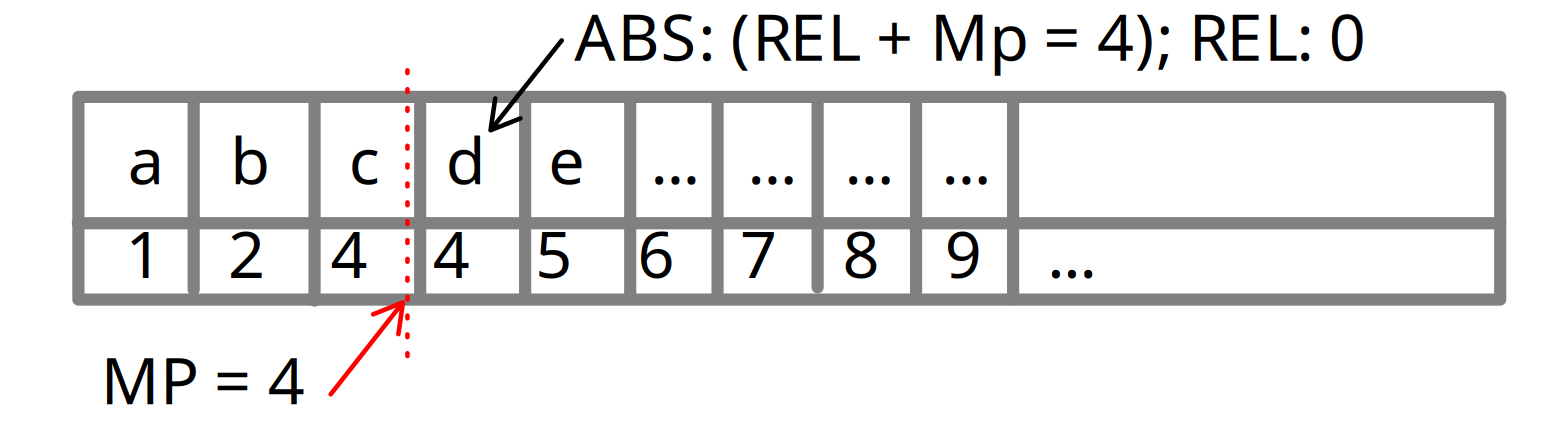
\includegraphics[width=\textwidth]{./vm_linmem_draft.png}
	\caption{\textcolor{red}{DRAFT:} Linear Memory of the rush VM}
	\label{fig:rush_vm_linmem}
\end{figure}

In order to get a deeper understanding of the addressing modes, a practical example can be considered.
The code in listing \ref{lst:rush_pointer_simple} displays a rush program in which a pointer to a variable is created.
First, the integer variable \texttt{num} is created.
In line 3, a pointer variable called \texttt{to\_num} is created by \emph{referencing} the \texttt{num} variable.

\TSListing[caption={Minimal Pointer Example in rush}, label={lst:rush_pointer_simple}, float=H]{listings/simple_pointer.rush}

In the rush VM, absolute addressing is only used for global variables and pointers.
Since a pointer specifies the address of another variable, its runtime value will be the absolute address of its target variable.
In the VM, the absolute address of a variable is calculated as soon as it is referenced using the \texttt{\&} operator.
For this purpose, the \texttt{reltoaddr} instruction exists.
This instruction calculates the absolute address of its operand and pushes the result onto the stack.
Here, the operand is the relative address of the variable to be referenced.
The listing \ref{lst:rush_pointer_simple_vm_instructions} shows the VM instructions generated from the rush program in listing \ref{lst:rush_pointer_simple}.

\TSListing[raw=true, caption={VM Instructions for the minimal Pointer Example}, label={lst:rush_pointer_simple_vm_instructions}, float=H]{listings/vm_instructions_simple_pointer.txt}

The first instruction \texttt{setmp} (\emph{set memory pointer}) increases the memory pointer by two.
This is because the \texttt{main} function contains two local variables whose space is to be allocated at the start of the function.
For instance, one might encounter \texttt{mp} being incremented by 0 since the corresponding function contains no local variables.
The next instruction \texttt{push} pushes the value 42 onto the stack.
In line 4, the \texttt{svari} (\emph{set variable immediate}) assigns the top value on stack to the specified relative address.
Here, 42 is popped off the stack since it is used by the \texttt{svari} instruction.
Next, the instruction stores the previously popped value at the relative address at the relative address 0 specified in the operand.
Now, the variable \texttt{num} with an initial value of 42 has been created.
Next, the \texttt{to\_num} variable is created by referencing the \texttt{num} variable.
In line 5, the \texttt{reltoaddr} (\emph{relative to address}) instruction is used to calculate the absolute memory address of the \texttt{num} variable.
This instruction calculates the absolute address of its operand at runtime using the algorithm described above.
Then, the instruction pushes the calculated address onto the stack so that it can be used by following instructions.
Here, the relative address 0 is used since the \texttt{svari} instruction has previously saved 42 at this location.
Therefore, the value of the variable \texttt{num} is saved at the relative address 0.
In line 6, the \texttt{svari} instruction is used again.
This time, it is used to save the value of the \texttt{to\_num} variable.
Since the absolute address of the referenced variable was previously calculated, it now exists on top of the stack.
Now, the instruction saves the absolute address of \texttt{num} at the relative address -1.
This is because the compiler targeting the VM assigns variables to higher relative addresses first.
The compiler then progresses into lower relative memory as more variables of the function are declared.
To summarize the above paragraph, this example uses relative addressing in order to declare local variables of a function.
However, absolute addressing is also used when variables are referenced in order to create pointers.
Therefore, each addressing mode serves a separate and important purpose.

\subsection{How the Virtual Machine Executes A rush Program}

By considering the minimal pointer example from above, we now have a rough idea how the VM might execute instructions.
In order to get a better understanding of how the rush VM works exactly, we will explain how it executes the program in listing \ref{lst:rush_vm_faster}.
For this, we should consider the instructions in Figure \ref{fig:tree_vs_vm} again.
The first instruction of the prelude function is \texttt{setmp}.
This instruction adjusts the memory pointer by the amount specified in the instruction's operand.
In this case however, the memory pointer remains unmodified since the operand of the instruction is 0.
Next, the \texttt{call 1} instruction calls the \texttt{main} function.
In order to understand how function calls work in this VM, we must consider the call stack of the rush VM.
Before the call-instruction, the caller pushes any call-arguments onto the stack so that they can be used as parameters by the callee.
Figure \ref{fig:rush_vm_call_stack} displays the state of the VMs call stack after the \texttt{call 1} instruction has been executed.
During execution of a call-instruction, the VM pushes a new stack frame onto its call stack.
Listing \ref{lst:call_frame_struct} shows how a call frame is implemented.

\TSListing[first line=26, last line=31, caption={Struct Definition of a \texttt{CallFrame}}, label={lst:call_frame_struct}, float=H]{deps/rush/crates/rush-interpreter-vm/src/vm.rs}

In this implementation, each call frame holds two important pieces of information.
In line 28 of listing \ref{lst:call_frame_struct}, the \texttt{ip} field is declared.
It specifies the \emph{instruction pointer} which holds the index of the current instruction.
Since the \texttt{call} instruction was interpreted previously, the instruction pointer of the new call frame is set to 0 as execution should continue at the first instruction of the called function.
The \texttt{fp} field is declared in line 30.
This field specifies the \emph{function pointer} which holds the index of the current function.

After the function call, \texttt{fp} is set to 1 since the main function is called and instruction should start at the first instruction of the main function.
Figure \ref{fig:rush_vm_call_stack} shows how the call stack of the VM looks like after the \texttt{call} instruction has been interpreted.
Function calls are managed in a stack in order to allow returning from functions.
If the VM encounters a \texttt{ret} (short for \emph{return}) instruction, it should leave the current function.
However, it should also know where to resume its fetch-decode-execute cycle.
For this, the VM just simply pops the top element from its call-stack.
Now, the top element on the stack contains the call-frame of the caller function.
In this call frame, \texttt{ip} still points to the \texttt{call} instruction which was responsible for calling the function.
Since \texttt{ip} is incremented automatically after most instructions, the VM resumes instruction execution at the first instruction after the call-instruction.
This way, function calls are implemented in a simple but robust manner.

% \begin{figure}[h]
% 	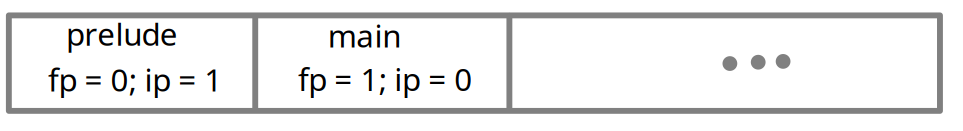
\includegraphics[width=\textwidth]{./vm_call_stack_draft.png}
% 	\caption{\textcolor{red}{DRAFT:} Call Stack of the rush VM}
% 	\label{fig:rush_vm_call_stack}
% \end{figure}

\begin{figure}
    \centering
    \begin{tikzpicture}
        \node[stack=3, rectangle split part align=center, text width=10ex, text centered, inner xsep=0]{
            \shortstack{prelude\\$fp=0$\\$ip=1$}
            \nodepart{two}{\shortstack{main\\$fp=1$\\$ip=0$}}
            \nodepart{three}{\ldots}
        };
    \end{tikzpicture}
	\caption{Call Stack of the rush VM}\label{fig:rush_vm_call_stack}
\end{figure}

Now that the call-instruction has been interpreted, the VM begins executing the first instruction of the main-function.
Since the main-function only calls the \texttt{rec} function with the argument 1000, there are no new concepts to consider in this function.
After the call instruction in line 7, the VM starts executing the instructions of the \texttt{rec} function.
At the beginning of the \texttt{rec} function, the memory pointer is incremented by 1.
This might seem erroneous since the \texttt{rec} function contains no visible variable declarations in its body.
However, this behavior is correct since function parameters count as variable declarations.
Since the function takes one parameter, the memory pointer is incremented by one cell.
Next, the instruction \texttt{svari} saves the value of the parameter which was previously pushed onto the stack at the relative address 0.
In line 12, the relative address of the memory cell containing the value of the parameter is pushed onto the stack.
It is then consumed by the \texttt{gvar} instruction in line 13.
At this point the top element on the stack contains an address-value referring to the target of the \texttt{gvar} instruction.
Therefore, the instruction first pops the top element from the stack.
In this case, the value of the popped element is the relative address 0.
Then, the instruction retrieves the value of the target variable and pushes it onto the stack.

In line 14, the constant value 0 is pushed onto the stack.
Next, the \texttt{eq} instruction pops two elements from the stack in order to test them for equality.
Then, the result of the comparison is pushed onto the stack as a boolean.
In this case, the instruction compares if the current value of \texttt{n} is equal to 0.
In line 16, the \texttt{jmpfalse} instruction is executed.
This instruction jumps to the specified instruction index if the value on top of the stack is \texttt{false}.
In this case, if the value on the stack is false, the parameter \texttt{n} was not equal to 0.
Now, the VM would jump to the instruction in line 19.
Here, the value of the parameter \texttt{n} is pushed onto the stack using the previously explained \texttt{push} and \texttt{gvar} instructions.
Now, the top item on the stack is the value of the parameter \texttt{n}.
In line 21, the \texttt{push} instruction pushes a constant 1 onto the stack.
Next, the \texttt{sub} instruction pops the first two elements from the stack in order to subtract their values from each other.
In this case, the instruction subtracts 1 from the value of \texttt{n} and pushes the result onto the stack.
Next, the \texttt{rec} calls itself recursively using a previously explained \texttt{call} instruction.
Since the call argument is the top element on the stack, the result of the subtraction is used as the argument of the recursive call.
Next, the function decrements the memory pointer in order to deallocate used memory using the \texttt{setmp} instruction in line 24.
At the end of a function, the memory pointer is always decremented by the amount it was incremented at the beginning of the function.
By deallocating the now unused memory, the compiler prevents the code from leaking memory at runtime.
Lastly, the \texttt{ret} instruction is used to return from the function.
Now we have considered what happens if the value of \texttt{n} was not equal to 0.

However, if the result of the comparison in line 15 is true, meaning that \texttt{n} is equal to 0, the \texttt{jmpfalse} instruction in line 16 does nothing.
In this case, the VM continues to the \texttt{push} instruction in line 17.
Here, the constant value 0 is pushed onto the stack.
Next, the VM interprets the \texttt{jmp} instruction in line 18.
Unlike \texttt{jmpfalse}, this instruction performs its jump without any condition.
In this case, the instruction jumps to the instruction at index 14 of the current function.
The instruction at index 14 is \texttt{setmp} in line 24.
Since functions also return values by placing them on top of the stack, the return-value would be 0 in this case.
Since we have covered what the instructions in the lines 24 and 25 do, we can summarize that the function returns the value 0 in this case.

Now that we have explained the semantic meaning of the instructions in Figure \ref{fig:tree_vs_vm}, we will explain how the fetch-decode-execute cycle works in the VM.
The code in listing \ref{lst:vm_run_meth} displays the \texttt{run} method of the rush VM.

\TSListing[first line=166, last line=177, caption={The \texttt{run} Method of the rush VM}, label={lst:vm_run_meth}, float=H]{deps/rush/crates/rush-interpreter-vm/src/vm.rs}

This method manages the entire fetch-decode-execute cycle of the VM.
It is immediately apparent that this method looks relatively simple considering that it plays such of a fundamental role in the VM.
Since the fetch-decode-execute cycle executes instructions repeatedly, the main construct in the function is a while-loop.
The condition of the loop checks that the current instruction pointer refers to a legal instruction inside the current function.
This way, the VM comes to a halt if it reaches the end of an instruction sequence.
In line 168, the next instruction to be interpreted is saved as the variable \texttt{instruction}.
This line represents the \emph{fetch} step since the next instruction is fetched from memory and placed in a spot where it can be used by the following steps.

In the body of the loop, the current instruction is executed using the \texttt{self.run\_instruction} method.
This method can return a runtime error, such as an integer-overflow error.
Furthermore, this method may return a integer representing the exit code of the program.
However, if the method returns none of these two possible types, the fetch-decode-execute cycle continues.
In this code however, one cannot observe the instruction pointer being incremented.
In order to answer the final question of how the current instruction is executed and the instruction pointer is incremented, we will now examine the code in listing \ref{lst:vm_run_instr_meth}.

\TSListing[first line=346, last line=359, caption={Parts of the \texttt{run\_instruction} Method of the rush VM}, label={lst:vm_run_instr_meth}, float=H]{deps/rush/crates/rush-interpreter-vm/src/vm.rs}

The code in listing \ref{lst:vm_run_instr_meth} displays the last part of the \texttt{run\_instruction} method.
This method mainly consists of an algorithm mathing the current instruction in order to execute specific code representing the instruction's semantic meaning.
In this example, the implementations of the \texttt{bitand} and \texttt{bitxor} instructions are visible.
Both instructions first pop two elements from the stack since they represent the operands of the underlying logical computation.
Then, a corresponding helper function is invoked on the left hand side operand.
The helper function then performs the actual computation of the logical operation.
Most of the infix-expressions are later executed in a similar way.
It is apparent that the execution of these instructions involves relatively little difficuilty.
After the instruction has been executed, the instruction pointer is finally incremented and nothing is returned.
For some special instructions, such as the jump-instructions, the instruction pointer should not be incremented since it would interfere with the jump.

\TSListing[first line=189, last line=192, caption={Execution of the \texttt{jmp} Instruction in the rush VM}, label={lst:vm_jmp_instr}, float=H]{deps/rush/crates/rush-interpreter-vm/src/vm.rs}

As seen in listing \ref{lst:vm_jmp_instr}, the \texttt{jmp} instruction only sets the instruction pointer to the target index specified in the instruction operand.
Then, the code returns from the method so that the instruction pointer is not incremented later.
This method represents both the \emph{decode} and \emph{execute} steps since it first matches (\emph{decode}) and then interprets (\emph{execute}) the current instruction.
Now that we have explained how some important parts of the rush VM work, we should now consider the compiler generating its input instructions.

\subsection{The Compiler Targeting the rush VM}

Since the rush VM interprets instructions directly, there must be a compiler translating the AST into these instructions.
For this purpose, we have implemented a compiler translating rush into instructions which can be understood by this VM.
Compared to the rush compiler targeting \emph{RISC-V},
implementation of this compiler has proven to be significantly simpler since the rush VM uses a stack-based design.
Since the VM's architecture was developed with the features of rush in mind,
the compiler sometimes requires suprisingly little effort for translating some AST-nodes. 
For instance, the compiler translates infix-expressions, such as $n + m$, into instructions using the \texttt{infix\_expr} method.
A part of this method is displayed in Listing \ref{lst:vm_compile_infix_expr}.

\TSListing[first line=538, last line=540, caption={Compilation of Infix-Expressions Targeting the VM}, label={lst:vm_compile_infix_expr}, float=H]{deps/rush/crates/rush-interpreter-vm/src/compiler.rs}

Here, the left hand side expression is compiled first.
Next, the right hand side is compiled too.
Finally, the appropiate arithmetic instruction is inserted.
The final instruction is generated by a helper function which converts an infix-operator into a matching instruction.
Most of the other compilers we have implemented for the rush project required significantly more code in order to implement the translation of infix-expressions.

\TSListing[first line=445, last line=450, caption={Compilation of Expressions Targeting the VM}, label={lst:vm_compile_expr}, float=H]{deps/rush/crates/rush-interpreter-vm/src/compiler.rs}

The code in Listing \ref{lst:vm_compile_expr} shows the top of the \texttt{expression} method in the VM compiler.
When we examine the method's signature, it becomes apparent that it only consumes an \texttt{AnalyzedExpresssion}.
However, the method does not return anything which represents the runtime value of the expression.
This is possible because the types of expression displayed in the listing are pushed onto the stack directly.
By pushing the values of atomic expressions onto the stack directly, most tree-traversing methods do not need to return values.
Due to this, short and elegant code like the one in listing \ref{lst:vm_compile_infix_expr} can be implemented.
In other compilers, the method responsible for compiling expressions usually returns the register which contains the value of the compiled expression at runtime.
This way, other parts of the compiled program can still use the runtime values of compiled expressions.

The rush VM includes a special instruction for the mathematical power operation (\texttt{**}).
Since many real architectures lack such a power instruction,
implementing a rush compiler targeting the VM has proven to be less demanding in this way.
On the opposite, many other rush compilers demanded implementation of special edge-cases in order to make compiling power-expressions feasible.
Furthermore, the VM also includes an \texttt{exit} instruction which terminates the fetch-decode-execute cycle instantly.
Here, the VM would come to a halt instantly, returning the top value on the stack as its exit code.
These examples showed how a carefully chosen target architecture simplies the implementation of its compiler by a great amount.

However, there is also one aspect of the VM which made implementation of the compiler targeting the VM more demanding than usual.
For instance, in most Assembly dialects, \emph{labels} can be used to allow jumps between blocks of code.
However, the VM intentionally does not support the use of such labels.
Since the VM would have to look up the exact instruction index of a label at runtime,
each jump targeting a label would involve some additional overhead.
This overhead is eliminated by the assembler during assembly of a program.
Since the assembler performs these lookups during translation,
the CPU does not have to deal with label lookups at runtime.
Like seen in the previous examples, jumping VM instruction require the exact index of the target instruction as their operands.
Therefore, the exact target index to which the instruction should jump must be known.
To illustrate this issue, we will consider how loops are implemented in the VM.
The rush code in Figure \ref{fig:vm_loops} presents a program containing a loop.
In the loop's body, the variable \texttt{n} is incremented by 1.
Next, the \texttt{break} keyword is used to terminate loop execution.
Therefore, the total amount of iterations is 1.

\noindent
\begin{figure}[h]
	\begin{minipage}{.5\textwidth}
		\centering
		\TSListing[frame=none]{listings/vm_basic_loop.rush}
	\end{minipage}%
	\begin{minipage}{.5\textwidth}
		\centering
		\TSListing[raw=true, frame=none]{listings/vm_basic_loop_instructions.txt}
	\end{minipage}
	\caption{How Loops are Interpreted by the VM}
	\label{fig:vm_loops}
\end{figure}

The rush VM instructions of the \texttt{main} function are displayed on the right side of Figure \ref{fig:vm_loops}.
Here, lines 2 and 3 are responsible for declaring the variable \texttt{n}.
The instructions in the lines 4-9 are used to increment the variable \texttt{n} by 1.
A new instruction which we have not covered so far is the \texttt{clone} instruction.
This instruction \emph{clones} the top item on the stack it without prior calls to \texttt{pop}.
Therefore, after the instruction has been executed, two idenical values exist on the top of the stack.
This instruction is only used in assign-expressions in order to duplicate the address value of the assignee variable.

After \texttt{n} is incremented, the instruction in line 10 jumps to the instruction index 11.
However, the last valid index is 10, it is represented by the \texttt{jmp 3} instruction.
If this occurs, the VM has no next instruction to fetch and therefore stops its fetch-decode-execute cycle.
Since this instruction jumps to a position outside the loop, it represents the \texttt{break} statement in line 5 of the source program.
The \texttt{jmp} instruction in line 11 is responsible for the repetition introduced by the loop.
This instruction jumps to the first instruction of the loop's body in line 4.
Therefore, the instructions inside the loop's body are executed repeatedly.
The difficuilty presented by this design is that the index of the jump's target instruction must be known before the target instruction is inserted.
The code in Listing \ref{lst:rush_vm_compiler_loop} displays a part of the method responsible for compiling loops for the rush VM.

\TSListing[first line=337, last line=343, caption={Implementation of Loops in the rush VM Compiler}, label={lst:rush_vm_compiler_loop}, float=H]{deps/rush/crates/rush-interpreter-vm/src/compiler.rs}

The statement in line 337 inserts the instruction responsible for jumping back to the start of the loop's body.
In line 340, the top loop is popped from the \texttt{loops} stack.
This stack is an internal field used by the compiler in order to save information about loops.
The top item on this stack always represents the loop currently traversed by the compiler.
Each loop saves two lists, each containing the indices of jump-instructions whose target index needs to be adjusted.
The first list contains the indices of jump-instructions generated by \texttt{break} statements
while the second lists saves instructions generated by \texttt{continue} statements.
For instance, if the compiler encounters a \texttt{break} statement, the code in listing \ref{lst:rush_vm_compiler_break} is executed.

\TSListing[first line=268, last line=273, caption={Compilation of \texttt{break} Statements in the rush VM Compiler}, label={lst:rush_vm_compiler_break}, float=H]{deps/rush/crates/rush-interpreter-vm/src/compiler.rs}

Here, the \texttt{pos} variable saves the index of the jump-instruction to be inserted.
In line 271, this index is then inserted into the list containing the placeholder indices of the current loop.
Lastly, the \texttt{jmp} instruction is inserted containing a placeholder target index.
Therefore, at the end of each loop's compilation, there will be a list containing the indices of instructions whose target indices need to be adjusted.
In line 342 of listing \ref{lst:rush_vm_compiler_loop}, the \texttt{self.fill\_blank\_jmps} method is used to set the target indices of the specified jump-instructions to \texttt{pos}.
We will omit the explaination of this method because it only iterates over the passed list of indices, replacing the target of the jump-instruction at the current index during the process.
Now, we have presented positive and negative aspects of writing a compiler targeting the rush VM.

As a conclusion, a VM is often a reasonable approach if an interpreted programming language is to be implemented.
The main advantages of a VM are increased speed and reduced memory usage at runtime.
The downsides include the need for a compiler targeting the VM, thus making its implementation more demanding. 


\chapter{Compiling to High-Level Targets}\label{chap:high_level_targets}
\section{Compilation to WebAssembly}

\begin{enumerate}
	\item what is WASM and why
	\item modules
	      \begin{itemize}
		      \item binary and text format (sections, leb128)
		      \item globals, functions, imports, exports, \ldots
		      \item uncommon to target binary format
	      \end{itemize}
	\item WASI
	\item basic implementation
	      \begin{itemize}
		      \item leb128
		      \item sections
		      \item \Verb{self.function_body}
	      \end{itemize}
	\item example program
\end{enumerate}

The first `external' compilation target presented here is \emph{WebAssembly}, or \emph{WASM} for short.
\TODO{research origins and goals of WASM and explain them here}
Unlike the name implies, WebAssembly is not only used in web applications.
By itself, it is only a specification that can be implemented by runtimes in any context.
Most modern browsers include such a WebAssembly runtime, but there are also standalone ones, for example \emph{wasmtime} and \emph{wasmer}.

\subsection{WebAssembly Modules}

Every valid WebAssembly file must contain exactly one module.
\TODO{confirm}
The WebAssembly specification defines two different representations for these modules.
First, there is a human-readable text representation, called \emph{WAT}\footnote{WebAssembly Text}, closely resembling S-Expressions\footnote{\TODO{what are S-Expressions}}.
This is comparable to assembly languages for CPU architectures and is the typical target for compilers.
Secondly, WebAssembly modules can also be represented using its binary format, which is optimized for size and comparable to the final binary files produced by assemblers.
Most often these binary modules are constructed from a text module by using a tool such as \emph{wat2wasm} from the \emph{WebAssembly Binary Toolkit (WABT)}.
However, the rush WebAssembly compiler instead opts to target the binary format directly, highlighting a few reasons for why most compilers should not do this.
Listing~\ref{lst:wat_demo_wat} and Listing~\ref{lst:wat_demo_hex} on page~\pageref{lst:wat_demo_wat} show the same basic WebAssembly module once as WAT and once as a commented hex dump of the same module in its binary representation as produced by \url{https://webassembly.github.io/wabt/demo/wat2wasm/}.

\Lirsting[float=p, label={lst:wat_demo_wat}, caption={Simple WebAssembly Module in Text Representation}]{listings/wat_demo.wat}
\Lirsting[float=p, label={lst:wat_demo_hex}, caption={Simple WebAssembly Module in Binary Representation}]{listings/wat_demo.hexdump}

Focusing on the text representation first, the shown module contains one function that takes two \qVerb{i32}s as parameters and returns a single \qVerb{i32}.
An \qVerb{i32} in WebAssembly represents an uninterpreted 32-Bit integer, that is, it is not clear whether the integer is signed or unsigned from the type itself.
Instead, values of this type can be interpreted as either signed or unsigned by different instructions.
For instance, the instruction \qVerb{i32.eq}, which checks for equality between two \qVerb{i32} values, behaves the same no matter the integer's signedness.
In contrast, \qVerb{i32.lt_s} and \qVerb{i32.lt_u} are two instructions both querying whether one \qVerb{i32} is less than another, once for signed and once for unsigned integers as denoted by the suffix.

The mentioned function is exported by the module under the name `addTwo' to make it accessible from outside.
What exactly `outside' is depends on the context the module is run in.
WebAssembly is \emph{stack based} and has one primary stack each instruction operates on.
The first two instructions of the `addTwo' function retrieve the local variable of the given index and push its value to the stack.
`Locals' in WebAssembly are simple values separate from the main stack.
Function parameters are always the first locals, but additional ones can be added, too.
After the two instructions ran, the stack now contains the values of the two function parameters.
They are then added by \qVerb{i32.add} which pops the top two elements off the stack and pushes the sum back on.
The return value implicitly is always what remains on the stack at the end of a function body.

Now focusing on the hex dump of the same module in binary in Listing~\ref{lst:wat_demo_hex}.
A WebAssembly binary file always starts with the four bytes \qVerb{00 61 73 6d} called the \emph{WASM binary magic} and representing a zero byte followed by the string `asm' using ASCII representation.
This is used by other programs to easily identify binary files as WebAssembly modules.
Following that is the version of the binary format, stored as a 32-Bit integer in Little-Endian\footnote{Little-Endian starts with the least significant byte first, whereas Big-Endian starts with the most significant byte}.
At the time of writing it is always `1'.

The binary module is then split into different sections each containing one kind of information about the whole.
Empty sections can be omitted.
Each section begins with its identifier, followed by the section size in bytes.
Most sections contain one vector of relevant data, and vectors always start with the count of elements they contain, and continue with the elements themselves.
The first section present here is the `Type' section.
It declares different types used by the module, most importantly, the function signatures.
The `Function' section then contains the number of functions of the current module and simply references to the `Type' section for each function's signature.
The module's exports are declared in the `Export' section.
Finally, the `Code' section contains the actual instructions for each function.
It is again stored as a vector, containing function bodies for all functions defined in the `Function' section in the same order.
Each function body begins with its size in bytes, continues with the instructions, and ended by an \qVerb{end} instruction represented by a \qVerb{0b} byte.

The `wat2wasm' tool used here additionally adds a custom `name' section.
Custom sections always have the ID `0' and must provide a custom name using ASCII.
This `name' section has its own specification separate from the main module specification, and is used to provide names for functions and variables that can then be used by development tools like `wasm2wat'.

Apart from exporting, WebAssembly modules can also import functions from outside.
Only the name and type signature must be provided and the WebAssembly runtime will then have to provide an implementation when running.
Furthermore, WebAssembly does not only have local variables, but also global ones, accessible from every function.
These must be initialized with some constant value and can either be mutable or immutable.

One may already have noticed that except for the version number at the start, all sizes, indices, lengths, and so on, have been stored using just a single byte.
But, this is not because those can only reach a maximum of 255, but instead WebAssembly uses the LEB128 encoding for integer literals in binary modules.
It is a space efficient way to store integers by only ever needing as many bytes as necessary for a number.
The encoding details are not explained here however, and our implementation for the rush compiler simply uses a pre-existing crate\footnote{A crate is a library in Rust terms} called `leb128'.

\subsection{The WebAssembly System Interface}

Since WebAssembly itself does not provide any guarantees about the runtime environment, it does not provide ways to interact with the environment, except, of course, for module imports and exports.
That is why an additional specification called the \emph{WebAssembly System Interface}, short \emph{WASI}, was created for WebAssembly modules that wish to communicate with an operating system.
Any runtime supporting WASI must provide a set of functions comparable to \emph{system calls} on Linux or Windows.
These can then be imported from a WebAssembly module to do things like writing to a console and exiting with a specific exit code.
Both wasmtime and wasmer implement the WASI interface.

A WebAssembly module making use of WASI must export one function under the name \qVerb{_start} that acts as the entry point.
The rush WebAssembly compiler only ever imports WASI's \qVerb{proc_exit} function which takes one 32-Bit integer as an argument and terminates execution with the given code.

\TODO{anything else to explain/mention here?}

\subsection{Implementation}

\Lirsting[ranges={324-328}, path prefix={deps/rush}, wrap=R, fancyvrb={numbers=right}, label={lst:wasm_instructions}, caption={Definition of Instruction Opcodes}]{deps/rush/crates/rush-compiler-wasm/src/instructions.rs}

The rush WebAssembly compiler directly targets the binary format.
This complicates compilation in a few ways, but removes the need for any external dependencies.
First, public constants are defined for all instructions and all types in separate files.
Listing~\ref{lst:wasm_instructions} shows an extract.

The \qVerb{Compiler} struct has a lot of fields for various purposes.
Only a few are shown in Listing~\ref{lst:wasm_compiler} and explained here.
To begin, a few fields regarding the currently compiled function are defined.
The \qVerb{function_body} contains the bytes with instructions for this function, and \qVerb{locals} stores which locals the function has along with their types.
In the binary format the locals are stored as a WebAssembly vector, that is, it starts with the number of locals, followed by each local.
Since the compiler cannot know the count of local variables beforehand, it stores them as a vector of byte vectors first.
This way, in the end it can first append the vector's length to the final output and then concatenate the contents.

\Lirsting[ranges={11-15, 26-31, 37-39, 58-58}, path prefix={deps/rush}, float=h, label={lst:wasm_compiler}, caption={\qVerb{Compiler} Struct Definition of the WebAssembly Compiler}]{deps/rush/crates/rush-compiler-wasm/src/compiler.rs}

\TODO{explain other shown fields}

\subsection{Example}

\TODO{example}

\section{Using LLVM for Code Generation}

LLVM is a software project intended to simplify the construction of a compiler generating highly-performant output programs.
It originally started as a research project by \emph{Chris Lattner} for his master's thesis at the University of Illinois at Urbana-Champaign~\cite{Lattner:MSThesis02}.
Since then, the project has been widely adopted by the open source community.
In 2012, the project was rewarded the \emph{ACM Software System Award}, a prestigious recognition of significant software which contributed to science.
From the point when popularity of the framework grew, it was renamed from \emph{Low Level Virtual Machine} to the acronym it is known by today.
Today, it can be recognized as one of the largest open source projects~\cite[preface]{Cardoso_Lopes2014-jt}.
Among many other projects, the Rust programming language depends on the LLVM compiler in order to generate its target-specific code~\cite[p.~373]{McNamara2021-hz}.
Furthermore, the \emph{Clang} C / C++ compiler uses LLVM as its code generating backend~\cite[preface]{Hsu2021-ez}.
Therefore, production ready compilers for popular programming languages have been implemented using the LLVM framework.
Besides open-source projects, many companies have also incorporated LLVM in their commercial software.
For instance, since 2005, Apple has started incorporating LLVM into some of its products~\cite[pp.~11-15]{Fandrey}.
A recent example of software developed by Apple which uses LLVM is the \emph{Swift} programming language which is mainly used for developing IOS apps~\cite[preface]{Hsu2021-ez}.

\subsection{The Role of LLVM in a Compiler}

In a compiler system, LLVM is responsible for generating target-specific code and performing optimizations.
The framework is known for performing very effective optimizations during code generation so that the translated program runs faster at runtime and uses less memory.
In order to use LLVM, the system provides and API which is usable by earlier steps of compilation.
Typically, a compiler frontend only analyzes the source program to create an AST.
Next, a separate step of compilation invokes the LLVM framework which carries on from this point\@.
This component traverses the AST and uses the API of LLVM in order to construct an intermediate representation of the program.
This way, the framework will be able to understand the semantic meaning of the program.
Next, LLVM compiles the input program to an output which is specific to an arbitrary target architecture.
As of today, LLVM features many target architectures so that a compiler designer does not have to worry about portability of the output program~\cite[preface]{Hsu2021-ez}.
Listing~\ref{fig:compilation_steps_llvm} shows how LLVM integrates into the previously discussed steps of compilation.
Therefore, the framework represents the \emph{back end} component of a compiler.

\begin{figure}[h]
	\centering
	\begin{tikzpicture}[node distance=3mm and 1cm, inner sep=3mm]
		\node (syntactic_analysis_text) [inner sep=0] {syntactical analysis};
		\node (lexical_analysis) [rec, below=of syntactic_analysis_text] {lexical analysis};
		\node (syntactic_analysis) [rec, fit={(syntactic_analysis_text) (lexical_analysis)}] {};

		\node (semantic_analysis) [rec, align=center, right=of syntactic_analysis] {semantic\\analysis};
		\draw [arrow] (syntactic_analysis) -- (semantic_analysis);

		\node (ir_generation) [rec, align=center, right=of semantic_analysis] {LLVM IR\\generation};
		\draw [arrow] (semantic_analysis) -- (ir_generation);

		\node (llvm) [rec, align=center, fill=gray!20, right=of ir_generation] {LLVM\\backend};
		\draw [arrow] (ir_generation) -- (llvm);
	\end{tikzpicture}
	\caption{Steps of Compilation When Using LLVM}\label{fig:compilation_steps_llvm}
\end{figure}

The updated Figure~\ref{fig:compilation_steps_llvm} now includes two new steps: \enquote{LLVM IR generation} and \enquote{LLVM backend}.
The first step generates the target-independent input used by the second step to generate target-specific code.
This step traverses the AST in order to generate a semantically equivalent program formulated using LLVM's intermediate representation.
A compiler writer must only implement the first three steps of this figure as the last step is represented by the framework itself.

\subsection{The LLVM Intermediate Representation}

The LLVM intermediate representation (\emph{IR}) represents the source program in a low-level manner.
However, even though this IR is low-level, it is still target-independent.
Furthermore, the IR also contains detailed type information which is usually uncommon for low-level representations of a program.
Therefore, high-level type information is preserved while the benefits of a low-level representation are introduced.
This allows LLVM to perform significant more aggressive optimizations compared to other compiler solutions or frameworks.
Therefore, programs compiled using LLVM as the backend will often run significantly faster due to the many aggressive optimizations introduced by the framework.

LLVM provides many APIs for interacting with the IR in memory.
This way, it can be created by a frontend without the need for a separate file containing the IR.
If the file containing the IR is written and read by the individual parts of the compiler,
the same performance issues introduced by multipass compilation would emerge.
Therefore, LLVM provides official APIs for the \emph{C++} and \emph{C} programming languages.
However, there are many unofficial bindings, such as for Rust, Go, or Python.
For instance, a compiler frontend written in Rust can leverage LLVM, although the system is written in C++.
Since LLVM must be able to perform complex program analysis before it can optimize a program,
its IR introduces many rules and constraints.
For instance, a program formulated using the IR should always obey the following hierarchy:

\begin{itemize}
	\item The top most hierarchical structure is the so-called \emph{module}.
	      It represents the current file being compiled.
	\item Each module contains several \emph{functions}.
	      Often, each function in the source program is represented using a function in the IR\@.
	\item Each function contains several \emph{basic blocks}.
	      A basic block contains a sequence of instructions.
	      Blocks should always be terminated using a jump, return, or unreachable instruction.
	      However, a basic block must never be terminated twice.
	\item Each basic block contains a sequence of \emph{instructions}.
	      Each instruction holds a semantic meaning and represents a part of the source program.
	      For instance, LLVM provides instructions for integer addition or function calls.
\end{itemize}~\cite[p.~211-213]{Hsu2021-ez}.

The IR provides a low-level enough representation in order to allow optimizations in the early stages of compilation.
However, due to the high-level type information contained in the IR,
LLVM is able to perform many aggressive optimizations on the IR during later stages of compilation.
This way, the framework can communicate a lot of information to the linker which can then use this information for \emph{link-time} optimizations.
The virtual instruction set of LLVM is therefore designed as a low-level representation with high-level type information.
This instruction set describes a virtual architecture which is able to represent an abstraction for most of the common types of processors.
Although it is low-level, the IR avoids machine specific constraints like registers or calling conventions.
Instead, the virtual architecture provides an infinite set of virtual registers which can hold the value of primitives like integers, booleans, floating-point numbers, and pointers.
All registers in the IR use the \emph{SSA}\footnote{Short for \enquote{static single assignment}, widely used in optimizing compilers} form in order to allow more optimizations.
In order to enforce the correctness of the type information included in the IR, the operands of each instruction all obey LLVM's type rules.
Therefore, LLVM only processes a program which contains valid type information~\cite[p.~14-17]{Lattner:MSThesis02}.

In order to understand how a program can be formulated using the LLVM IR, we consider the rush program for calculating Fibonacci numbers again.
For reference, the rush program used in this example can be found in Listing~\ref{lst:rush_fib} on page~\pageref{lst:rush_fib}.
The code in Listing~\ref{lst:llvm_fib} displays the identical rush program formulated in LLVM IR\@.
The IR was generated by the LLVM targeting rush compiler\footnote{Generated in Git commit \rushCommit{}, automatically built with this document}.
This compiler is presented in a later chapter since right now, only its output is of relevance.
The IR displayed in this listing shows a module named \qVerb{main}.

\Lirsting[ranges={1-30}, caption={LLVM IR Representation of the Program in Listing~\ref{lst:rush_fib}}, label={lst:llvm_fib}, float=h]{listings/generated/fib.ll}

In the lines 5 and 23, two functions are defined using the \qVerb{declare} keyword.
It is apparent that the functions in the LLVM module represent the functions from the source rush program.
The function's name in the IR matches the name in the source file as it increases readability of the program.
When examining the signature of the \qVerb{fib} function in line 5 of the IR,
it becomes apparent that the function returns a runtime value of the type \qVerb{i64}.
In rush, the \qVerb{int} type represents a 64-bit signed number.
Therefore, the \qVerb{i64} LLVM type represents the rush \qVerb{int} type.
Furthermore, we can observe that the function takes a parameter named \qVerb{\%0} of the type \qVerb{i64}.
It represents the `\texttt{n}' parameter in the rush source program.

In line 6, the start of the \qVerb{entry} block of the \qVerb{fib} function is declared using the block's name followed by a colon.
Since LLVM can perform more optimizations on variables if they are declared in the \qVerb{entry} block of a function,
the rush compiler uses the \qVerb{entry} block solely for variable declarations.
In line 7, the \qVerb{icmp slt}\footnote{Short for \enquote{integer compare (signed less than)}} is used in order to compare the runtime value of the parameter `\texttt{\%0}' to a constant 2.
The boolean result is then saved in a virtual register named `\texttt{\%i\_lt}'.
Since LLVM's virtual registers may have arbitrary names,
the rush compiler uses names which will make reading of the generated IR easier.
In line 8, the block is terminated using the \qVerb{br}\footnote{Short for \enquote{branch}} instruction.
The instruction will only jump under the condition that the value of `\texttt{\%i\_lt}' is true.
%Here, we can see that LLVM instructions are able to operand on different type of operands depending on what the instruction should do.
Here, the \qVerb{merge} and the \qVerb{else} labels are used as operands of the branch-instruction.
Conditional jumps in LLVM always require an alternative jump to perform if the condition is false at runtime.
Due to constraints introduced by its internal optimizations, LLVM only allows jumps to target blocks contained in the same function.
Therefore, two labels of blocks in the current function are used as the operands of this instruction.
As the names \qVerb{merge} and \qVerb{else} suggest, this branch-instruction presents the essential part of the if-expression in the source program.
If the condition was true at runtime, the instruction would jump to the \qVerb{merge} block in line 10.
What might seem odd is that there is no \qVerb{if} block.
In fact, the rush compiler has even compiled this block into LLVM IR\@.
However, since that block only jumped to the \qVerb{merge} block, LLVM's optimizations removed it entirely.

In line 11, of the \qVerb{merge} block, the \qVerb{phi} instruction is used.
These so called $\phi$-nodes are necessary due to the SSA form used in the IR\@.
In short, a \emph{phi-node} produces a different value depending on the basic block where control came from.
Since the if-construct is an expression in rush, LLVM must know if the result of the \qVerb{entry} or the \qVerb{else} branch is to be used as the result of the entire if-expression.
As a solution to this problem, these phi-nodes associate a value to an origin branch.
In this example, the phi-node yields the value of the parameter `\texttt{\%0}' (\qVerb{n}) if control came from the \qVerb{entry} block.
In the source program, \qVerb{n} should be returned without modification if it is less than 2.
Therefore, the runtime result of the phi-node is `\texttt{\%0}' if it is less than 2 at runtime.
Otherwise, if control came from the \qVerb{else} block, the phi-node's result is taken from the virtual register `\texttt{\%i\_sum3}'.
However, we have not covered where this virtual register is declared.
For this, we consider the instructions in the \qVerb{else} block, starting in line 15 with the `\texttt{add}' instruction.
In this case, the instruction subtracts 2 from the parameter `\texttt{\%0}' and saves the result in `\texttt{\%i\_sum}'.
However, an addition instruction using a negative operand is used since LLVM's optimization decided that this instruction is likely beneficial.
This is done in order to create the argument value for the first recursive call to \qVerb{fib}.
Next, the \qVerb{call} instruction is used in order to perform the recursive call.
Here, the `\texttt{\%i\_sum}' register is used as an argument to the call-instruction.
The return value of the function call is saved in the `\texttt{\%ret\_fib}' register.
The same behavior is used in order to call \qVerb{fib(n - 1)}.
However, in that case, 1 is subtracted from the parameter and saved in `\texttt{\%i\_sum1}'.

Next, the \qVerb{add} instruction in line 19 is used in order to calculate the sum of the return values of the recursive calls
This sum is then saved in the virtual register `\texttt{\%i\_sum3}'.
Therefore, this register is used in the phi-node in line 11 so that the result of the recursive calls is used as the result of the if-expression.
Next, the \qVerb{br} instruction jumps to the `\texttt{merge}' block.
However, this jump happens unconditionally since the instruction does not consider a condition and only has one target label.
After the jump to the \qVerb{merge} block, the previously explained $\phi$-node is encountered.
Finally, the \qVerb{ret} instruction in line 12 is used in order to use the result of the if-expression as the return-value of the function.
Since the \qVerb{main} function does not introduce any new concepts, we will omit detailed explanation of its contents.
However, in line 27, the \qVerb{unreachable} instruction is used in order to state that it is never executed.
This is necessary because LLVM requires that every basic block is terminated at its end.
The `\texttt{exit}' function terminates the program using a system call and therefore terminates the basic block.
However, LLVM does not regard call-instructions as diverging and therefore disallows the call to \qVerb{exit} as a way to terminate the basic block.
Since LLVM does not know that the \qVerb{exit} function terminates program execution, an \qVerb{unreachable} instruction is inserted to communicate a block termination to LLVM\@.

It is to be mentioned that the original IR generated by the rush compiler looks slightly different because LLVM has already performed all of its aggressive optimizations on this code.
By considering the example from above, it became apparent that the IR represents many source language constructs in a high-level way.
For instance, function calls can be used without considering the complex rules introduced by low-level calling conventions.
Here, calling and returning from a function can be implemented using very little effort.
Furthermore, virtual registers allow the compiler frontend to omit register allocation entirely.
Lastly, the LLVM IR can subjectively be seen as very readable since registers, basic blocks, and functions may contain custom, human-readable labels.
Moreover, most instructions have a relatively reasonable name which allows readers to guess what the instruction is doing without them reading any LLVM documentation.

\subsection{The rush Compiler Using LLVM}

In order to get acquainted to the LLVM framework practically, we have implemented a rush compiler which uses the framework as its backend.
However, the first problem emerged soon since the LLVM project only provides official C / C++ bindings to be used by other programs.
Nonetheless, the entire rush project is written in the Rust programming language.
Therefore, a third-party Rust wrapper around LLVM is required.
We have settled on using the \emph{Inkwell} Rust crate since it exposes a safe rust API for using LLVM for code generation~\cite{Inkwell2023}.

\Lirsting[ranges={26-29,47-47}, caption={Parts of the Struct Definition of the rush LLVM \qVerb{Compiler}}, label={lst:llvm_cmp_struct}, wrap=L, wrap width={.5\textwidth}]{deps/rush/crates/rush-compiler-llvm/src/compiler.rs}

This compiler uses the annotated AST generated by the semantic analyzer in order to translate it into LLVM IR\@.
Here, each type of AST node is translated using its own individual function.
For instance, an expression AST node is translated into IR by the \qVerb{expression} method of the compiler.
This way, translation of individual AST nodes can be organized in order to increase maintainability.
To understand how this rush compiler leverages LLVM in order to translate programs, we should first consider some implementation details.
The code in Listing~\ref{lst:llvm_cmp_struct} displays the top part of the `\texttt{Compiler}' struct definition.

The \qVerb{context} field in line 27 represents a container for all LLVM entities including modules.
Next, the \qVerb{module} field contains the underlying LLVM module.
In line 29, the \qVerb{builder} field contains a helper struct provided by Inkwell which allows generation of IR solely in memory.
All the types of the above fields are provided by the Inkwell crate and are therefore used to interact with the framework.
In order to get a deeper understanding of how this compiler works exactly, we will now consider how the program in Figure~\ref{fig:llvm_simple} is translated into IR.

\noindent
\begin{figure}[h]
	\begin{minipage}{.5\textwidth}
		\centering
		\Lirsting[fancyvrb={frame=none}]{listings/simple.rush}
	\end{minipage}%
	\begin{minipage}{.5\textwidth}
		\centering
		\Lirsting[ranges={5-18}, fancyvrb={frame=none}]{listings/generated/simple.ll}
	\end{minipage}
	\caption{Translation of a Simple rush Program to LLVM IR}\label{fig:llvm_simple}
\end{figure}

The source program on the left side contains the `\texttt{foo}' and the `\texttt{main}' functions.
These functions are declared in the lines 5 and 14 of the output IR\@.
The `\texttt{foo}' function takes two parameters (`\texttt{n}' and `\texttt{m}').
It uses the two parameters and calculates their sum in order to use it as the exit code of the program.
In line 7 of the IR, the parameter `\texttt{n}' and the variable `\texttt{m}' are added together.
What strikes the eye is that the declaration of `\texttt{m}' cannot be seen in the IR\@.
Instead, the constant value 3 of the variable is used in the addition instruction.
Therefore, the program uses less memory since a redundant mutable variable is not saved in memory.
This again shows how advanced LLVM optimization is and how it benefits the program.
The result of this addition is then used in order to call the `\texttt{exit}' function.
This function call takes place in line 8 of the IR\@.
Therefore, the exit code of the program will be 5.
During translation, the compiler first iterates over all declared functions in order to add them to the LLVM module.
Listing~\ref{lst:llvm_main_fn} displays parts of the method responsible for translating the `\texttt{main}' function.

\Lirsting[ranges={321-321,334-351,369-371}, caption={Compilation of the `\texttt{main}' Function Using LLVM}, label={lst:llvm_main_fn}, float=H]{deps/rush/crates/rush-compiler-llvm/src/compiler.rs}

In the lines 334--336, the `\texttt{main}' function is added to the current LLVM module.
The definitions of the variables `\texttt{fn\_name}' and `\texttt{fn\_type}' are not visible.
The first variable specifies the name of the function to be inserted, while the latter describes the function's signature.
The return type of the function is specified by the `\texttt{fn\_type}' variable.
In most cases, the return-type of the function is an integer since C libraries can then use the function as its `\texttt{main}' function.
In cases where the generated code should not depend on C libraries, `\Verb|fn_name|' will be `\Verb|_start|' and `\Verb|fn_type|' will state that the function returns \emph{void}.
In the lines 339 and 340, this method adds the `\texttt{entry}' and `\texttt{body}' basic block.
Next, the `\texttt{entry}' and `\texttt{body}' block are appended to the newly created function.
Therefore, the main-function now contains these two basic blocks.
In the lines 343--347, the `\Verb|curr_fn|' field of the compiler is updated.
This field holds information about the current function being compiled.
In line 345, the `\Verb|llvm_value|' field is of particular importance since all later additions of basic blocks, e.g., during loop compilation require an Inkwell `\texttt{FunctionValue}'.
Therefore, this field of the current function can later be accessed if a basic block should be appended.
Furthermore, the `\Verb|entry_block|' field in line 346 is used every time a pointer is declared.
However, the reason for this behavior is explained later.

Using the Inkwell crate, most instructions generated will be automatically appended to the end of the current basic block.
Therefore, the position of the instruction builder is changed to the end of the newly created `\texttt{body}' block.
Since this block contains the beginning of the main-function's body, the `\texttt{block}' method of the compiler is called in line 351.
In this case, this method first creates a new scope, then compiles all the statements which the block contains.
Lastly, the method attempts to compile the block's optional expression.
If the content of the body of the main-function does not lead to the insertion of more basic blocks,
the `\texttt{body}' block will contain the entire contents of the function after the method call.

In line 2 of the example rush program, the `\texttt{main}' function calls the \texttt{foo} function using the argument value 2.
In order to understand how this compiler translates function calls, we will now consider Listing~\ref{lst:llvm_call}.

\Lirsting[ranges={916-916,951-954,957-957}, caption={Compilation of Call-Expressions Using LLVM}, label={lst:llvm_call}, float=H]{deps/rush/crates/rush-compiler-llvm/src/compiler.rs}

The code in Listing~\ref{lst:llvm_call} displays a small part of the `\Verb|call_expr|' method of the rush LLVM compiler.
This snipped shows the statement inserting the LLVM `\texttt{call}' instruction.
For this, the `\Verb|build_call|' method of the builder is called using the target function, call arguments, and the name of the result register.
Since the variable `\texttt{func}' represents the called function, it was previously declared by looking up the function name in the module.
The `\texttt{args}' variable is of type `\Verb|Vec<BasicMetadataValueEnum>|' and therefore represents a list of Inkwell values representing the arguments used for the call.
This variable was also defined previously by iterating over the \qVerb{node.args} vector containing expressions.
This vector is contained in the provided AST node representing the call-expression.
Each argument expression is then compiled, and its result is placed into the `\texttt{args}' output vector.
However, we cannot understand how results of expressions are handled in this compiler without considering Listing~\ref{lst:llvm_exprs}.

\Lirsting[ranges={873-879,910-912}, caption={Compilation of Expressions Using LLVM}, label={lst:llvm_exprs}, float=H]{deps/rush/crates/rush-compiler-llvm/src/compiler.rs}

The code in Listing~\ref{lst:llvm_exprs} shows parts of the \texttt{expression} method of this compiler.
When consider the method's signature, it becomes apparent that it uses an `\texttt{AnalyzedExpression}' in order to generate a `\texttt{BasicValueEnum}'.
The return type of the function is of particular importance.
Using Inkwell, most inserted instructions yield a symbolical value at compile time.
This value represents a virtual register which will contain a real \emph{value} at runtime of the program.
Therefore, the `\texttt{BasicValueEnum}' returned by the function represents the virtual register which will hold the result of the expression at runtime.
This way, symbolical values can be used at compile time, thus presenting a high-level abstraction for generating the IR\@.
The lines 875--879, show how a constant integer expression is compiled.
Here, a constant int value of the `\texttt{i64}' type is created and transformed into a `\texttt{BasicValueEnum}' which is then used as the method's return value.
For more complex expressions, the `\texttt{expression}' method invokes other methods which are specialized on this type of expression.
For instance, if an infix-expression like `\texttt{3 * n}' is compiled, this method calls the `\Verb{infix_expr}' method in line 910.
Here, the current AST node is passed to the specialized function as a call argument.

\Lirsting[ranges={1021-1024}, caption={Compilation of Integer Infix-Expressions Using LLVM}, label={lst:llvm_infix}, float=H]{deps/rush/crates/rush-compiler-llvm/src/compiler.rs}

The code in Listing~\ref{lst:llvm_infix} shows a part of the `\Verb|infix_helper|' method which is responsible for compiling parts of infix-expression.
Line 1021 contains the code for inserting the `\texttt{mul}' multiplication instruction.
Here, the variables `\texttt{lhs}' and `\texttt{rhs}' are used as arguments for the `\Verb|build_int_sub|' method call.
They, too, represent virtual registers which will contain the value of the left- and right-hand side at runtime.
Furthermore, the string containing `\Verb|i_prod|' specifies the name of the virtual register containing the product of the multiplication performed by the instruction.
In this example, compiling basic integer multiplication has proven to be really simple since only one instruction needs to be inserted.
This simplicity applies to most infix operations performed on integers.
However, compiling mathematical power operations has proven to be more demanding since LLVM does not provide an instruction for performing these operations.
Line 1024 is executed if the method needs to compile such an integer power operation.
In order to mitigate this issue, the `\Verb|__rush_internal_pow|' method is called instead of a method provided by Inkwell.
This method first declares the `\Verb|core::pow|' function in order to call it directly after.
This function implements an algorithm for power operations given an integer base and exponent.
However, this function is implemented in IR directly by hardcoding the required calls to Inkwell into this function.
Therefore, even complex calculations like this one can be implemented even though LLVM does not provide a straight-forward way to accomplish them directly.

In line 6 of the source program, a let-statement is used to declare the mutable variable `\texttt{m}' with the initial value 3.
However, there is never a value assigned to this variable.
This variable is only mutable so that the compiler has to use stack memory for it.
Non-mutable variables are inlined by the compiler in order to save resources during runtime.
In order to understand how the compiler translates let-statements, we will now consider Listing~\ref{lst:llvm_let}.

\Lirsting[ranges={609-624,629-630}, caption={Compilation of Let-Statements Using LLVM}, label={lst:llvm_let}, float=h]{deps/rush/crates/rush-compiler-llvm/src/compiler.rs}

The code in Listing~\ref{lst:llvm_let} displays parts of the `\Verb{let_stmt}' method of this compiler.
This method is responsible for compiling let-statements.
In line 610, the initializer expression of the statement is compiled.
The `\texttt{rhs}' variable then specifies the virtual register which contains the result of the expression at runtime.

The code in the block after line 614 is only executed if the variable was declared as mutable.
Otherwise, the variable would be constant and therefore require no space in memory.
Therefore, in order to present relevant code in this example, the `\texttt{m}' variable in the source program had to be declared as mutable.
In line 616, the `\Verb{alloc_ptr}' method is used in order to create a new Inkwell pointer value.
The first argument of the call specifies that the name of the pointer should be identical to the name of the variable.
The second argument passes the type of the initializer expression to the method.
The statement in line 619 is used in order to insert a store instruction.
Here, the instruction should store the value of the initializer expression in the newly created pointer.
Since pointers present a way to use stack memory, also non-pointer variables in the source program are internally compiled to an IR program using pointers.
Finally, in line 622, the newly defined variable is inserted into the current scope of the compiler.
Every variable inside the scope saves its Inkwell value and its type since these fields are required when the variable is used later.
The code in Listing~\ref{lst:llvm_ptr_alloc} shows the `\Verb{alloc_ptr}' method of the compiler.

\Lirsting[ranges={635-649}, caption={Pointer Allocation in the LLVM Compiler}, label={lst:llvm_ptr_alloc}, float=h]{deps/rush/crates/rush-compiler-llvm/src/compiler.rs}

This method exists in order to create a new Inkwell pointer value.
Like hinted previously, pointers are declared in the `\texttt{entry}' block of each function in order to allow for more aggressive optimizations.
In line 640, this method places the builder cursor at the end of the entry-block of the current function.
Next, in line 643, a `\texttt{alloca}' LLVM instruction is inserted.
This instruction is responsible for allocating a new pointer which points to stack memory.
After the instruction has been inserted, the builder position is reset to where it was before the method was called.
Finally, the pointer is returned so that it is usable for other parts of the compiler.

\subsection{Final Code Generation: The Linker}\label{sec:linker}

After LLVM has compiled a program, it outputs an \emph{object file} representing the compiled source program.
Object files contain the binary machine code output of a compiler or an assembler.
In the case of LLVM, they contain the target-specific machine code generated from the intermediate representation.
There are many different formats for representing object files, such as \emph{ELF} on Unix-like systems.
However, object files are usually still \emph{relocatable}\footnote{Load addresses of position-dependent code may still be changed} and not directly executable.
In order to create an executable program from object files, a \emph{linker} is used.

A linker or \emph{link editor} is a program which takes one or more object files in order to combine them into a single file.
Often, the output of the linker is a file which can be executed by the operating system.
For instance, a linker might take an object file generated by a compiler in order to create the final executable program.
During \emph{linking}, a linker often perform numerous tasks, such as \emph{relocation} or \emph{symbol resolution}.
For instance, a linker might also include \emph{library code} in the executable if the object file depends on external functionality provided by that library.
A common example for this library code is the functionality provided by a C standard library.
In order to combine these modules, an essential part of the liker's actions is presented by relocation and code modification~\cite[pp.~1-15]{Levine2000}.
During relocation, the linker assigns definitive addresses to numerous parts of the program.
Relocation is required, for instance, when the program to be translated consists of multiple modules referencing each other.
Here, the order in which the individual parts of the program will be placed in memory is not known.
Therefore, any absolute addresses in the program are not determined~\cite[p.~74]{Zhirkov2017-wk}.
However, we will not explain these concepts further since they are not of particular relevance for understanding the purpose of a linker.

\begin{wrapfigure}{R}{0.5\textwidth}
	\centering
	\begin{tikzpicture}[node distance=2cm]
		\node(linker)[center] {Linker};
		\node(obj)[entity, left of=linker, yshift=2cm] {Object files\\(\texttt{*.o})};
		\node(libs)[entity, right of=linker, yshift=2cm] {Libraries \\ (\texttt{*.a} / \texttt{*.so})};
		\node(cmd)[text width=2.8cm, right of=linker, xshift=1.25cm] {Command line arguments};

		% TODO: Maybe use `arrow` instead of `relation` in order to remove spacing
		\draw [relation] (obj) -- node[anchor=west] {} (linker);
		\draw [relation] (libs) -- node[anchor=west] {} (linker);
		\draw [relation] (cmd) -- node[anchor=west] {} (linker);

		\node(exe)[entity, below of=linker] {Executable \\ file};
		\draw [relation] (linker) -- node[anchor=west] {} (exe);
	\end{tikzpicture}
    \caption{How a Linker Works}{\cite[p.~7]{Levine2000}}\label{fig:linker}
\end{wrapfigure}

The shell command in Listing~\ref{lst:ld_llvm} presents an example liker invocation.
In this example, the LLVM compiler has generated an object file named \texttt{input.o}.
The flag \texttt{-dynamic-linker} is used in order to tell the linker which dynamic linker should be used.
Next, some library files in the directory `\texttt{/usr/lib/}' are included.
These files belong to an implementation of the C standard library and are required so that the `\texttt{exit}' function works properly.
Furthermore, the `\texttt{input.o}' file is specified so that the linker includes it.

\Lirsting[caption={Using LD to link the LLVM output}, label={lst:ld_llvm}, float=H]{listings/invoke_ld.sh}

This way, the shell command would generate an executable program named `\texttt{output}' from an object file named `\texttt{input.o}'.
Therefore, a linker often presents the final step of translating a source program into an executable which the computer can understand.
However, the linker is completely independent of the previous stages of compilation and is therefore not displayed in the figures.
Even though the linker program \emph{LD} is used in this example, the choice of the linker is completely irrelevant as long as the linker supports the program generated by the compiler.

\subsection{Conclusions}

As a conclusion, implementing a compiler which leverages LLVM presents a lot of advantages.
For instance, the language will be able to support many backend architectures.
Most of the demanding work is being done by LLVM, therefore implementing the compiler will proof to be less difficult and error-prone.
Moreover, LLVM performs a lot of very effective optimizations which would otherwise have to be implemented by the compiler designer.
However, these optimizations often involve a lot of work and are therefore unpractical to implement for simpler languages.
Therefore, LLVM presents a robust, production-ready, and scalable backend which is even used in real-world compilers.
However, by depending on LLVM, the resulting compiler will often be less portable since cross-compilation still presents an issue if used across programming language boundaries.

Finally, in order to understand how LLVM's optimizations can positively impact application performance at runtime, we will consider the Fibonacci benchmark again.
In this benchmark, the 42nd Fibonacci number is calculated using the program displayed in Listing~\ref{lst:rush_fib} on page~\pageref{lst:rush_fib}.
However, the 10 in line 2 was replaced by a 42.
Running a binary compiled using the rush LLVM compiler took around 1.3 seconds.
However, executing the binary generated using the rush x86\_64 compiler took around 2.17 seconds\footnote{Average from 100 iterations. OS: Arch Linux, CPU: Ryzen 5 1500, RAM: 16 GB}.
Therefore, the program compiled using LLVM ran roughly 1.66 times faster.


\chapter{Compiling to Low-Level Targets}\label{chap:low_level_targets}
\section{Low-Level Programming Concepts}

% chktex-file -2
\newpage

\section{\riscv{}: Compiling to a Modern RISC Architecture}

The \emph{\riscv{}} \emph{ISA}\footnote{Short for: \enquote{instruction set architecture}} is a new and modern \emph{reduced instruction set} architecture focussing on simplicity and expandability.
The initial version was developed at \emph{UC Berkely} in the context of another related research project.
Since its introduction in 2011, the architecture has been rapidly growing in popularity.
Since the beginning, the project has been managed and led by the \emph{\riscv{} foundation}, consisting of many individuals contributing to the project.
Today, corporate members of the \riscv{} foundation include companies like \emph{Google}, \emph{Microsoft}, \emph{Samsung}, and \emph{IBM}.
Therefore, the general popularity and commercial attraction of the technology is apparent.
However, unlike most previous ISAs, the \riscv{} architecture is a completely \emph{open-source} project and is therefore not controlled by a single large corporate entity.
This can be regarded as a large competitive advantage over other popular RISC architectures like \emph{ARM}.
In the past, many ISAs have failed due to them being too restrictive with their licensing, thus preventing widespread commercial adoption.
However, \riscv{} is completely open and free to use, so that many companies like \emph{Google} can leverage the technology commercially while contributing to the project.
Unlike most of the previous ISAs, which were developed during the 1970s or 80s, \riscv{} is one of the few which were developed this decade.
Therefore, it seems like \riscv{} could be a significant architecture to be used in all sorts of devices in the near future~\cite[preface]{Patterson2017}.

\subsection{Register Layout}

\begin{wraptable}{r}{.4\textwidth}
	\centering
	\caption{Common registers of the \riscv{} architecture.}{\cite[p.~155]{Waterman2019}}\label{tbl:riscv_regs}
	\begin{tabularx}{\linewidth}{l|L}
		\rowcolor{gray!10} Register   & Purpose                         \\ \hline
		\texttt{zero}                 & Hardwired zero                  \\ \hline
		\texttt{ra}                   & Return address                  \\ \hline
		\texttt{sp}                   & Stack pointer                   \\ \hline
		\texttt{t0} —  \texttt{t6}    & Temporary                       \\ \hline
		\texttt{fp}                   & Frame Pointer                   \\ \hline
		\texttt{a0}, \texttt{a1}      & Function argument, return value \\ \hline
		\texttt{a2} — \texttt{a7}     & Function argument               \\ \hline
		\texttt{s1} — \texttt{s11}    & Saved register                  \\ \hline
		\texttt{fa0}, \texttt{fa1}    & FP args, return value           \\ \hline
		\texttt{fa2} — \texttt{fa7}   & FP args                         \\ \hline
		\texttt{fs0} — \texttt{fs11}  & FP saved registers              \\ \hline
		\texttt{ft0} —  \texttt{ft11} & FP temporaries                  \\
	\end{tabularx}
\end{wraptable}

Most RISC architectures typically have a large count of registers~\cite[Chapter~2]{Dandamudi2005}.
When compared to other popular architectures, the truth of this statement becomes clear.
For instance, the \emph{x86\_32} architecture has 8 registers.
The popular RISC architecture \emph{ARM-32} provides twice that amount, meaning 16 registers.
However, a \riscv{} CPU includes 32 registers, which is drastically more than the previously mentioned architectures.
Moreover, these 32 registers only include registers holding integer values.
Just for floating-point numbers, the ISA even provides another 32 registers.
Like previously explained, using more registers usually leads to increased efficiency of the output program.
Therefore, a register allocation algorithm targeting the \riscv{} architecture could be more aggressive compared to one targeting x\_86 for instance~\cite[p.~10]{Patterson2017}.

The Table~\ref{tbl:riscv_regs} shows most of the registers which the \riscv{} architecture provides.
For this table, the official ABI names of the registers have been used in order to make this section easier to read.
The first column of the table contains a register's name while the second column describes its purpose.

The first row of the table contains the \qVerb{zero} register.
On \riscv{}, this register is special.
Like its name suggests, it holds the value of a constant 0.
Unlike other registers, it is read-only, meaning that it can never be overwritten, therefore preventing accidental writes.
In the next row, the \qVerb{ra} register is shown.
It saves the \emph{return address} of a function or subroutine.
If a return-instructions is used, the value in \qVerb{ra} is read as it is used to jump to a specific instruction.
The purpose of this register is elaborated further in Subsection~\ref{sec:riscv_calling_conv} about \riscv{}'s calling convention.
The \qVerb{sp} and \qVerb{fp} registers are used for managing stack memory.
Their purpose is explained in Subsection~\ref{sec:riscv_stack} about stack memory.
In the fourth row, the \qVerb{t0} — \qVerb{t6} are displayed.
These registers are often used to store temporary values used in larger computations.
In row six, the registers \qVerb{a0} and \qVerb{a1} can be seen.
These both serve as call arguments and return values of functions.
The remaining a-registers \qVerb{a2} — \qVerb{a7} can only be used as function call arguments.
How functions are called using registers will be explained in Subsection~\ref{sec:riscv_calling_conv}.
The next row contains the \emph{saved} registers \qVerb{s1} — \qVerb{s11}.
These registers are typically preserved across function calls, meaning a called function must not overwrite them.
What the previously explained registers have in common is that they all hold integer values.
Depending on the exact \riscv{} architecture, all registers, including floating-point registers, either hold 32 or 64 bits of information.
For floating-point number values, \riscv{} provides other registers.
These registers are able to hold floating-point numbers according to the \emph{IEEE 754--2008} standard~\cite[Chapter~11]{Waterman2019}.
Just like their integer counterparts, the floating-point registers \qVerb{fa0} and \qVerb{fa1} are used as function call arguments and as return values.
However, the other fa-registers \qVerb{fa2} — \qVerb{fa7} can only be used as function arguments holding floating-point numbers.
Just like the \qVerb{sx} registers, the \qVerb{fs0} — \qVerb{fs11} registers are usually preserved across function calls.
Last, the \qVerb{ft0} — \qVerb{ft11} registers can be used as temporary registers for floating-point numbers.
It is apparent that the floating-point registers are provisioned very similarly to the integer registers.
Therefore, a programmer or compiler targeting the architecture can utilize roughly the same principles,
regardless of the data-type stored in each register~\cite[pp.~18f,p.~34]{Patterson2017},~\cite[p.~155]{Waterman2019}.

Now, it has become apparent that \riscv{} includes many registers which are grouped into semantic categories.
Every category is meant to be used in the specified manner, however, these groups are mostly only a suggestion of how each register should be used.
Although this subsection provides a good overview over the registers of the architecture, the purpose of some special registers is still not known.
These special registers, like \qVerb{sp}, \qVerb{fp}, and \qVerb{ra}, are thoroughly explained in the next sections.

\subsection{Memory Access Through the Stack}\label{sec:riscv_stack}

\begin{wrapfigure}{L}{0.39\textwidth}
	\hspace{-3.25cm}
	\begin{tikzpicture}[scale=.9]
		\small
		% TODO: also use longer arrow in top `fp_main`?
		\stackTopFixed{...} \cellcom{\scriptsize 24(sp\textsubscript{main})} \cellptr{\scriptsize \tt fp\,$_\text{main}$}
		\startframe
		\cell{fp} \cellcom{\scriptsize 16(sp\textsubscript{main})}
		\cell{ra} \cellcom{\scriptsize 8(sp\textsubscript{main})}
		\cell{a: int} \cellcom{\scriptsize -24(fp\textsubscript{main})} \cellptrA{\scriptsize \texttt{sp\,$_\text{main}$}}
		\cell{b: char} \cellcom{\scriptsize -25(fp\textsubscript{main})} \cellptrA{\scriptsize \texttt{fp\,$_\text{foo}$}}
		\finishframe{\tt main}
		\startframe
		\cell{fp} \cellcom{\scriptsize 8(sp\textsubscript{foo})}
		\cell{ra} \cellcom{\scriptsize 0(sp\textsubscript{foo})} \cellptrA{\scriptsize \texttt{sp\,$_\text{foo}$}}
		\finishframe{\tt foo}
		% TODO: uncomment the line below?
		%\stackbottom
	\end{tikzpicture}
	\caption{Example stack layout in \riscv{}.}\label{fig:riscv_basic_stack}
\end{wrapfigure}

As mentioned in the dedicated subsection about the stack, it presents a way to save data outside of registers.
This subsection explains special conventions followed when using stack memory on \riscv{}.
Just like previously explained, most stacks are accessed through the specialized pointers.
On \riscv{}, there is a \emph{stack pointer} which is saved in the \qVerb{sp} register.
Furthermore, the \qVerb{fp} register contains the \emph{frame pointer}.

Like most memory stacks, the \riscv{} stack grows downwards, meaning it progresses into lower memory regions.
In the current implementation of the rush \riscv{} compiler, the stack pointer points to the last legal memory cell of the current stack frame.
Therefore, \qVerb{sp} points on the cell with the lowest address of the current stack frame.
On the other hand, the frame pointer \qVerb{fp} points to the cell above the end of the current stack frame.
Therefore, the frame pointer always points to a memory cell which is illegal to use by the current function.
Thus, a stack frame is defined by its upper and lower bounds, represented by \qVerb{fp} and \qVerb{sp}, respectively.

In order to understand how the above behavior is used in practice, Figure~\ref{fig:riscv_basic_stack} is to be considered.
Furthermore, the rush program in Listing~\ref{lst:rush_riscv_stack} should be considered.

\Lirsting[caption={A rush program containing two variables.}, label={lst:rush_riscv_stack}, float=H]{listings/riscv_stack.rush}

This snipped shows a rush program which contains two functions.
In the \qVerb{main} function of this program, two variables are defined.
The \qVerb{a} variable holds the integer value 42 while the \qVerb{b} variable contains the char value \qVerb{z}.
In line 4, the \qVerb{foo} function is called.
Figure~\ref{fig:riscv_basic_stack} shows the state of the stack at the point when this function was called.
The braces on the left side of the stack group the stack into frames.
On the right side of each stack cell, its relative address can be observed.
As explained previously, each stack cell is accessible either by offsetting \qVerb{sp}
or \qVerb{fp}. The stack pointers of each stack frame can are displayed by the arrows on the right side of the stack.

The stack shown in this figure contains two frames, one for each function involved in the call.
Since the \qVerb{main} function is called first, it is displayed at the top of the figure.
Normally, the last pushed element of a stack is located at the top, however, just as described,
this stack progresses towards lower memory, meaning that it grows downwards.
Since the \qVerb{main} function calls the \qVerb{foo} function, the stack frame for the \qVerb{foo} function is located at the bottom of the stack.

It is apparent that every stack frame saves the \qVerb{fp} and \qVerb{ra} registers at its top position.
These two special registers are saved at the two top positions of each call before any of the code in the function's body is executed.
Why these registers are saved on the stack is explained in Subsection~\ref{sec:riscv_stack} about the calling convention.
Since every stack frame contains these two elements,
the minimum size $s$ of a \riscv{} stack frame in bytes must be $s = \frac{2 \times \text{Size}\,_\text{int}}{8}$.
Since $s$ is dependent on the integer-size of the \riscv{} architecture, the minimum required memory differs per \riscv{} architecture.
For instance, if the 64-bit version of \riscv{} was used, the minimum size would be 16 bytes ($s = \frac{2 \times 64}{8} = 16$).
However, if the 32-bit version of the architecture was used, $s$ would be only 8 bytes ($s = \frac{2 \times 32}{8} = 8$).

Additionally, one can observe that the \qVerb{main} function's
stack frame contains cells which save the two variables which are defined in the body of the function.
Since the code in the function's body (where the variables are defined) is executed after \qVerb{fp} and \qVerb{ra} have been saved on the stack,
the cells containing these variables appear lower in the stack.
Another interesting observation is that the more recently declared variables are also saved in lower cells of the stack frame.
Therefore, the order in which variables are saved in the stack follows the \emph{LIFO} principle which is common in stacks.

In this example, in the stack frame of the function \qVerb{main}, the registers \qVerb{fp} and \qVerb{ra} require 16 bytes of memory together.
Therefore, the variable \qVerb{a} can be saved at the next 8 bytes of memory, meaning -24(fp).
This way, the variable is saved at the memory region from -24(fp) until the start of -16(fp) or 16(sp) in this example.
Therefore, each stack cell requires exactly as much memory as shown in the figure.
Just like described earlier, different rush types require different quantities of memory.
A character for instance only uses 1 byte of memory.
Thus, the entire variable \qVerb{b} is saved at -25(fp), meaning one byte below the end of the variable \qVerb{a}.
This way, each variable only uses as much memory as it actually requires.

However, the question of how the compiler is able to keep track of saved variables remains.
For this, the compiler maps a variable's name to a memory location.
To be precise, the compiler contains a \emph{HashMap} which associates a variable's name with its \qVerb{fp} offset.
In case of the program in Listing~\ref{lst:rush_riscv_stack}, the variable \qVerb{a} is associated with a \qVerb{fp} offset of -24.
If the variable is referenced at a later point, the compiler performs a simple lookup of the variable's memory address.

\subsection{Calling Convention}\label{sec:riscv_calling_conv}

\begin{wrapfigure}{R}{0.42\textwidth}
	\centering
	\begin{tikzpicture}[node distance=5mm]
		\node(stack)[
			vstack=6,
			rectangle split part fill={none, none, gray!20, gray!20, none, none},
			rectangle split part align=left,
		]{
			\nodepart{one}{{\texttt{\tiny 24(sp\textsubscript{0})}} fp$_0$}
			\nodepart{two}{{\texttt{\tiny 16(sp\textsubscript{0})}} ra$_0$}
			\nodepart{three}{{\texttt{\tiny 08(sp\textsubscript{0})}} argument 2}
			\nodepart{four}{{\texttt{\tiny 0(sp\textsubscript{0})}} argument 1}
			\nodepart{five}{{\texttt{\tiny 8(sp\textsubscript{1})}} fp$_1$}
			\nodepart{six}{{\texttt{\tiny 0(sp\textsubscript{1})}} ra$_1$}
		};
		\draw [thick, dashed] ([xshift=-.5cm, yshift=-.33cm]stack.four west) --  node[anchor=west, xshift=2cm, align=center] {\scriptsize function\\ \scriptsize boundary} ([xshift=.5cm, yshift=-.33cm]stack.four east);

		\node(sp)[left of=stack, xshift=-2.2cm, yshift=-0.32cm, align=left] {\scriptsize SP$_0$ \\ \scriptsize FP$_1$};
		\draw[arrow, shorten >= 2pt](sp) -- (stack.four west);

		\node(fp)[left of=stack, xshift=-2.2cm, yshift=2.26cm] {\scriptsize FP$_0$};
		\draw[arrow, shorten >= 2pt](fp) -- ([yshift=.74cm]stack.one west);

		\node(sp)[left of=stack, xshift=-2.2cm, yshift=-1.6cm] {\scriptsize SP$_1$};
		\draw[arrow, shorten >= 2pt](sp) -- (stack.six west);
	\end{tikzpicture}
	\caption{Spilled registers during a \riscv{} function call.}\label{fig:riscv_call_spill}
\end{wrapfigure}

Just like previously explained, most architectures provide a calling convention which dictates how low-level function calls should be managed.
For most architectures, the calling convention is part of the ISA's official specification.
In the case of \riscv{}, the calling convention is specified in a separate document~\cite{RiscvABI2022}.

The first step of calling a function involves placing the arguments in a place where the function can access them.
For \riscv{}, this involves placing the arguments into specialized registers.
Like described in the Table~\ref{tbl:riscv_regs}, only special classes of registers can be used as call arguments.
For integer arguments, the first arguments are placed in the registers \qVerb{a0}--\qVerb{a7}
For instance, the first two arguments of the rush function call
\qVerb{foo(40, 2, 3.14)} would be placed in the registers \qVerb{a0} and \qVerb{a1}.
However, the third argument is a floating-point number and can therefore not be placed inside an integer register.
Therefore, the first floating-point argument register \qVerb{fa0} contains the argument \qVerb{3.14}.
In this case, all arguments can be held in regisers and spilling would not be required.

In case the function accepted nine or more integer arguments,
all further integer arguments upward of the ninth position would have to be spilled on the stack.
Here, the successive registers \qVerb{a0}--\qVerb{a7} would contain the first eight integer arguments of the called function.
The argument at position 9 however is then spilled on the stack since there are no registers left which could contain the additional argument~\cite[p.~8]{RiscvABI2022}.

The Figure~\ref{fig:riscv_call_spill} displays a possible state of the call stack during a function call which uses ten integer arguments.
If ten integer arguments are used, two arguments would have to be spilled on the stack.
In the figure, the spilled registers are placed in the stack cells \enquote{argument 1} and \enquote{argument 2}.
Here, the cell \enquote{argument 1} would hold the ninth argument while \enquote{argument 2} holds the tenth argument.
Therefore, all spilled argument registers will be placed in the stack frame of the caller function.
Normally, variables saved on the stack are aligned to reflect their sizes.
In case of spilled argument registers however, every argument will occupy exactly 8 bytes on the stack, even if the data type itself requires less space.

Now that the first step of a procedure call is explained, the question of how the second step works in \riscv{} remains.
In the second step, the underlying procedure call is made using a specialized instruction.
In \riscv{} assembly, one typically uses the call \emph{pseudoinstruction}\footnote{A macro generating multiple instructions from one pseudoinstruction. Therefore, the actual count of ISA instructions remains low while convenience features can be used in assembly~\cite[p.~68]{Dandamudi2005}.}.
Due to a lack of functions in assembly, the call-instruction uses the name of its target label as one operand.
Therefore, labels can be called as if they were functions.
This instruction will jump to the first instruction of the specified target label while saving the address of the next instruction after the \qVerb{call} instruction in the register \qVerb{ra}~\cite[p.~22]{Patterson2017}.
As hinted previously, the \qVerb{ra} register saves the \emph{return address}.
Therefore, the return address is set every time a function call is performed.

During the third step of the function call, the called function acquires local storage resources.
To be precise, the function decrements the stack pointer by the amount required by the stack frame.
Therefore, the function allocates as much stack space as required for storing local variables and other data.
Additionally, the frame pointer and return address are saved on the stack so that nested function calls do not cause issues.
For instance, if the return address was not saved on the stack, a nested function call would overwrite its stored value.
In this case, the parent function could no longer return since the return address now holds an incorrect value.
In order to mitigate issues like this, the return address and frame pointer are saved on the stack.
Figure~\ref{fig:riscv_call_spill} shows that the two registers are saved at the two positions on the top of the new stack frame.
This part of the function is often called the \emph{prologue} as it is executed before any of the function's internal code.

After the code of the function has been executed, the so-called \emph{epilogue} is executed.
Since the frame pointer and return address have been saved on the stack during the prologue,
the epilogue restores these registers by loading their values from the stack.
Furthermore, the amount which was subtracted from the stack pointer in the prologue is now added to the pointer in order to restore it to its original state before the function call.
Here, incrementing the stack pointer represents deallocating the previously acquired stack space.
However, the memory in the stack frame is not actually deleted since only the stack pointer is modified.
Even though the used memory is not explicitly deleted, it is still freed since it will probably be overwritten by the next function call.
If the prologue would not save the return address on the stack, a nested function call would overwrite the return address of the parent function, therefore creating a bug~\cite[p.~33]{Patterson2017}.
By saving the return address on the stack, nested function calls do not cause difficulties.
It is apparent that this design contains a lot of similarities to the call-stack of the rush VM\@.
However, in the VM, the process of saving and restoring the return address was managed automatically by the VM,
whereas, here, the programmer has to manually pay attention to saving and restoring this important piece of data.
Therefore, implementing function calls is definitely more demanding in \riscv{} assembly than in the rush VM\@.

In case a function returns a value, it must be communicated to the caller so that it can access it.
For integer-based types, the first return value of a function is placed in the register \qVerb{a0}
while floating-point numbers are placed in the register \qVerb{fa0}.
This way, the caller code can obtain a function's return value by accessing the \qVerb{a0} and \qVerb{fa0}
registers respectively. If a function does not return a value, these steps are just omitted.
It is to be mentioned that character and boolean values are also placed inside the \qVerb{a0} register since these types can be represented by integers.

Lastly, the epilogue contains a return-instruction which should jump to the place where the function was called.
This \emph{ret} instruction reads the value stored in \qVerb{ra} in order to jump to this address.

\subsection{The Core Library}

Like hinted in the section about the linker on page~\pageref{sec:linker},
a program might use functionality provided by external libraries.
In case of the rush \riscv{} compiler, external functions are used for character-arithmetic,
the mathematical power operator, and the system \emph{exit} call.
Since these concepts must introduce additional logic, the compiler should not be emitted their instructions every time they are used.
In that case, the repeated emission of redundant instructions would result in enlarged and unnecessary complex output code.
In order to mitigate these issues, the compiler simply inserts call-instructions referencing external functions.
External functions can be called just like any other function, however, their definition is not found in the same assembly file.
As described previously, resolving these external calls is later handled by the linker.
For this compiler, we later refer to this target specific library code by the term \emph{corelib}.

For instance, a function for mathematical power operations is implemented in the corelib.
Therefore, the compiler can emit a procedure call to this method every time rush's \qVerb{**} operator is used in the source program.
For this project, the entire corelib is written in \riscv{} assembly.
However, it is often rational to implement a corelib or standardlib using a high-level language like C.
Since the corelib's functions are specified in separate files, they are packaged into an \emph{archive file} which is later used by the linker.
The assembly code in Listing~\ref{lst:riscv_exit_corelib} shows the implementation of the \qVerb{exit} subroutine in the \riscv{} corelib.
The task of this subroutine is to invoke a specific functionality the Linux kernel by performing a \emph{system call}.

\Lirsting[float=H, ranges={8-12}, caption={The assembly implementation of the \qVerb{exit} subroutine.}, label={lst:riscv_exit_corelib}]{deps/rush/crates/rush-compiler-risc-v/corelib/src/exit.s}

A \emph{system call} (often abbreviated to \emph{syscall}) is an invocation of a function of operating system's kernel.
In Linux, more than 90 percent of the available system calls are implemented on all architectures.
A common system call is \qVerb{exit}.
This function terminates the current process and performs various cleanup steps.
Its first parameter is the exit status (or code) which can be checked by the shell or other programs~\cite[p.~148]{Love2013}.
In \riscv{} Linux, the integer representation of a call to \qVerb{exit} is 93~\cite{Torvalds1991}.

In line 8 of Listing~\ref{lst:riscv_exit_corelib}, the \qVerb{exit} label is declared as global using the \qVerb{.global} directive.
Next, the \qVerb{exit} label is declared in line 10.
In line 11, the \qVerb{li} instruction is used in order to place 93 in the value \qVerb{a7}.
On \riscv{} Linux systems, the content of the \qVerb{a7} register specifies the type of syscall to be performed.
Here, 93 is placed inside this register since it represents the \qVerb{exit} syscall.
In line 12, the \qVerb{ecall} instruction is used in order to call the program's environment~\cite[p.~23]{Patterson2017}
Here, this call invokes the Linux kernel.
In this example, some \riscv{} assembly code was shown.
The next subsection explains these concepts and idioms in more detail.

\subsection{\riscv{} Assembly}

The Listing~\ref{lst:riscv_simple} shows a rush program containing two functions and a global variable.
In line 1 of the rush program, the mutable global variable \qVerb{m} is defined with the initial value 42.
In line 4 of the main-function, \qVerb{m} is incremented by 1.
Next, in line 5, the \qVerb{foo} function is called using \qVerb{m} as the only call argument.
In line 6, a \qVerb{return} statement is used to terminate the main-function explicitly.
The body of the \qVerb{foo} function only contains a call to the \qVerb{exit} function.
Therefore, the \qVerb{foo} function only exits using the specified parameter \qVerb{n} as the exit code.
In this case, the exit code of the displayed program will be 43.
The code in Listing~\ref{lst:riscv_simple_asm} on page~\pageref{lst:riscv_simple_asm} shows the output assembly generated from this program by the rush \riscv{} compiler\footnote{Generated using Git commit \rushCommit{}.}.
Because the assembler code of the \qVerb{foo} function would take up too much space in the assembler program, it is intentionally omitted from this listing.
Since the excluded function does not introduce any new concepts anyway, omitting it will not lead to a loss of explained concepts.

\Lirsting[float=H, caption={Example rush program containing two functions.}, label={lst:riscv_simple}]{listings/riscv_simple.rush}

\begin{wrapfigure}{L}{0.5\textwidth}
	\centering
	\Lirsting[ranges={1-31, -4 53-56}, fancyvrb={frame=none}]{listings/generated/riscv_simple.s}
	\caption{Compiler output from the rush program in Listing~\ref{lst:riscv_simple}.}\label{lst:riscv_simple_asm}
\end{wrapfigure}

In line 1, the \qVerb{.global} assembler directive is used to declare the global symbol \qVerb{_start}~\cite[p.~36]{Patterson2017}.
On most architectures, the \qVerb{_start} label indicates a program's entry point, therefore marking the first instruction to be executed~\cite[p.~19]{Zhirkov2017-wk}.
In line 5, the \qVerb{_start} label is defined by placing a colon after its name.
In line 6, the \qVerb{call} instruction is used to call the \qVerb{main..main} function.
What strikes the eye here is that the already familiar \qVerb{main} function is prepended by the \qVerb{main..} prefix.
Since this rush compiler implements name mangling\footnote{Compilers often \emph{mangle} names in order to create a unique name for every function~\cite[pp.~119-120]{Levine2000}},
every function declared in a rush program will contain this prefix.
However, unlike high-level function calls in LLVM, this call instruction is used alongside the previously explained low-level calling conventions of \riscv{}.

In the next line, the \qVerb{li} instruction is used to load the constant integer 0 into the register \qVerb{a0}~\cite[reference card]{Patterson2017}.
Like explained in the previous section about the \riscv{} calling convention,
the register \qVerb{a0} is used for the first integer call argument.
In line 8, the \qVerb{exit} function is called, however, one cannot see the definition of this function in the current file.
This is because the exit function is provided by the rush \riscv{} corelib which was explained previously.
Since 0 was previously placed inside the register for the first integer call argument, the \qVerb{exit} function is called using 0 as the argument.
Therefore, the instructions in the lines 7--8 are responsible for terminating the program using the exit code 0.
These two instructions are always inserted at the end of the \qVerb{_start} label in order to terminate the program appropriately in case the rush code does not call \qVerb{exit} on its own.
This is required in order to prevent a segmentation fault which occurs if the program is not terminated properly.

Due to the function call in line 6, we will now shift our focus on the \qVerb{main..main} label in line 10.
In line 11, the first line of the \qVerb{main} function, a comment indicates the beginning of the function's prologue.
Just like demanded by the \riscv{} calling convention, the rush compiler emits code for a \emph{prologue} and an \emph{epilogue} for each function.

As described in the previous sections about calling conventions, one task of the prologue is allocating stack space.
In this prologue, the \qVerb{addi} instruction in line 12 subtracts 16 from the value stored in \qVerb{sp}.
Since subtraction is used, the stack pointer is decremented, leading to the stack progressing into lower memory.
Therefore, this instruction increases the size of the stack, thus allocating memory.
Here, an addition instruction is used even though subtraction is required.
In \riscv{}, the \qVerb{addi} instruction requires one register and one immediate value as its operands.
Due to the third operand being an \emph{immediate} value, the trailing \qVerb{i} (\emph{immediate}) appears in the instruction's name.
Since this immediate value can be negative, an additional instruction for immediate subtraction is redundant~\cite[reference card]{Patterson2017}.
This example shows how the \riscv{} ISA omits redundant instructions in places where it is feasible.
In this case, the stack pointer is decremented by 16 since two 8-byte values are stored on the stack in the lines 13 and 14.
Just like described in the previous subsection about the stack, these registers are always saved on the stack.

The comment in line 17 indicates the start of the function's body.
First, the previously explained \qVerb{li} instruction in line 18 places a constant 1 in register \qVerb{a0}.
Next, the \qVerb{ld} instruction in line 19 is used in order to load the value of the global variable \qVerb{m} into the register \qVerb{a0}~\cite[reference card]{Patterson2017}.
Global variables, like \qVerb{m} in this example are saved under the \qVerb{.rodata}. section or under the \qVerb{.data} section if they are mutable.
In this example, \qVerb{m} is not declared as mutable and therefore saved under the \qVerb{.rodata} section.
The start of the \qVerb{.rodata} section is represented by the \qVerb{.section} assembler directive found in line 53.
Here, a label called \qVerb{m} is defined.
In this label, the \qVerb{.dword} directive is used to define the global initializer value of the variable.
In \riscv{}, this directive stores 64 bit of information in successive memory doublewords~\cite[p.~39]{Patterson2017}.
The initializer value of the global variable is 42 and is represented as \qVerb{0x2a} using hexadecimal in the assembly code.
Since these data labels require their contents to be specified in hexadecimal, the trailing comment shows the base 10, human-readable version of the number.
Because global variable are not saved on the stack, special instructions like \qVerb{ld} are required to interact with global variables stored in the program's data sections.

At this point, the register \qVerb{a0} would contain 1 and \qVerb{a1} would contain 42.
In line 20, the \qVerb{add} instruction is used in order to save the sum of \qVerb{a0} and \qVerb{a1} in the register \qVerb{a2}.
Now, the value saved in \qVerb{a2} would be 43.
Next, the \qVerb{sd} instruction in line 21 saves the value of the register \qVerb{a2} at the memory location of the global variable \qVerb{m}, meaning that \qVerb{m} is updated to reflect its new value 43.
It now becomes apparent that these instructions are responsible for the add-assign expression in line 4 of the rush program.
Another interesting observation is that the last operand of the \qVerb{sd} instruction specifies the temporary register \qVerb{t6}.
The instruction uses this register for saving temporary data during the process of saving data in \qVerb{m}~\cite[reference card]{Patterson2017}.

In line 22, the previously explained \qVerb{ld} instruction is used in order to load the value of the same variable into the register \qVerb{a0}.
Then, the \qVerb{call} instruction in line 23 is used in order to call the \qVerb{foo} function using the value of m as its argument.
However, one cannot easily observe how call arguments are passed here.
Like explained previously, the first integer argument of a function call must be placed in the register \qVerb{a0}.
Since \qVerb{m} was loaded into \qVerb{a0} previously, it will be used as the call argument for \qVerb{foo} automatically.
Therefore, the \qVerb{foo} function is called using 43 as the first argument.

Since the \qVerb{foo} instruction only calls the \qVerb{exit} function, its explanation will not be beneficial for introducing new concepts.
Therefore, we will omit the explanation of the assembler output of the \qVerb{foo} function.
The final instruction of the main-function's body is the \qVerb{j} instruction in line 24.
This instruction will cause the CPU to jump to the address of the specified label.
In this example, the CPU will jump to the first instruction of the \qVerb{epilogue_0} label~\cite[p.~17]{Patterson2017}.
Therefore, the rush compiler uses the \qVerb{call} instruction for jumps caused by function calls and the \qVerb{j} instruction for jumps between blocks of the current function.

Like explained previously, every function has a \emph{prologue} and an \emph{epilogue}.
Since one of the tasks handled by the epilogue is releasing resources allocated by the prologue, the function's stack pointer is incremented in line 30.
Finally, the \qVerb{ret} instruction in line 31 is used in order to jump back to the instruction whose address is specified in the \qVerb{ra} register~\cite[reference card]{Patterson2017}.

\subsection{Supporting Pointers}

In Subsection~\ref{sec:pointers}, we have explained how pointers can be used in rush.
Since every rush backend should support all features of the language, pointers also need to be implemented for the \riscv{} architecture.
In order to get a rough understanding of how pointers work in this compiler, the code in Listing~\ref{lst:rush_simple_pointer} and~\ref{lst:rush_simple_pointer_asm} are to be considered.

\begin{minipage}{.34\textwidth}
	\center
	\Lirsting[float=H, fancyvrb={frame=none}, caption={Example rush program containing a pointer.}, label={lst:rush_simple_pointer}]{listings/rush_simple_pointer.rush}
\end{minipage}%
\hspace{3cm}
\begin{minipage}{.45\textwidth}
	\center
	\Lirsting[float=H, fancyvrb={frame=none}, ranges={10-10,18-24}, caption={\riscv{} assembly output generated from Listing~\ref{lst:rush_simple_pointer}.}, label={lst:rush_simple_pointer_asm}]{listings/generated/riscv_rush_simple_pointer.s}
\end{minipage}


The code in Listing~\ref{lst:rush_simple_pointer} shows a rush program in which a variable is referenced to create a pointer which is then dereferenced.
In line 2, the mutable variable \qVerb{a} is defined using an initial value of 42.
Next, in line 3, the variable is referenced in order to use the resulting address to define the variable \qVerb{to_a}.
In line 4, the \qVerb{to_a} pointer variable is dereferenced in order to use the value of \qVerb{a} as the exit code of the program.


Listing~\ref{lst:rush_simple_pointer_asm} includes the most significant part of the compiler output which represents this rush program\footnote{Generated using Git commit \rushCommit{}.}.
In line 18 of this listing, the integer value 42 is placed in the register \qVerb{a0}.
Next, \qVerb{a0} is saved on the stack at \qVerb{-24(fp)} using the \qVerb{sd} instruction.
Like the comment suggests, the instruction in line 20 is used in order to reference a.
Here, the \qVerb{addi} instruction is used to subtract 24 from the value stored in the \qVerb{fp} register.
The result of this subtraction is saved in the register \qVerb{a0}.
Therefore, the register now contains the absolute memory address of the \qVerb{a} variable.
Since the syntax \qVerb{-24(fp)} means that the variable is saved at $fp - 24$, the subtraction uses the exact same information which is already known about the variable.
Here, instead of using the saved memory location of the variable like \qVerb{x(fp)}, the information is used in order to calculate the absolute address of the target variable.
This computation can only be performed at runtime since the value of \qVerb{fp} is not known at compile time.
In line 21, the \qVerb{a0} register which contains the memory address is also saved on the stack.
Therefore, the \qVerb{a} variable is saved at \qVerb{-24(fp)} while \qVerb{to_a} is saved at \qVerb{-32(fp)}.

In order to access the value of \qVerb{a}, \qVerb{to_a} is dereferenced in line 4 of the rush program.
For this, the memory address stored in the variable \qVerb{to_a} first needs to be loaded from the stack.
Here, the \qVerb{ld} instruction in line 22 of the assembly output is used.
The instruction will load the memory address stored at \qVerb{-32(fp)} (in \qVerb{to_a}) into the \qVerb{a0} register.
Next, another \qVerb{ld} instruction in line 23 is used in order to load the value of the variable saved at the previously fetched memory address.
What strikes the eye is that \qVerb{0(a0)} instead of \qVerb{x(fp)} is used for specifying the target memory address of the load instruction.
In this case, \qVerb{0(a0)} means that the instruction should load its value from the address saved in \qVerb{a0} with an offset of 0.
Since an offset of 0 is used, the practical description of the instruction is that it loads a value saved at the memory address specified in \qVerb{a0}.
Because \qVerb{a0} contains the memory address of the \qVerb{a} variable, the instruction loads 42 into the \qVerb{a0} register.

\subsection{The rush Compiler Targeting \riscv{} Assembly}

Just like the other compilers presented in this paper, this one also traverses the annotated AST using the postorder technique.
Unlike the LLVM or WASM compiler, this compiler emits \riscv{} assembly files which are later assembled by the assembler.

\subsubsection{Struct Fields}

Before any complex code samples can be considered, important struct fields of the compiler first need to be explained.
The rust code in Listing~\ref{lst:riscv_compiler_attr} shows important struct fields of the rush compiler targeting \riscv{}.

\Lirsting[ranges={11-11,15-15,19-34}, caption={Fields of the \riscv{} \qVerb{Compiler} struct.}, label={lst:riscv_compiler_attr}, float=H]{deps/rush/crates/rush-compiler-risc-v/src/compiler.rs}

In line 15, the field \qVerb{blocks} is declared.
This field holds a vector containing values of the type \qVerb{Block}.
That type provides an abstraction representing a label with its basic block in the assembly output.
Therefore, this struct needs to contain a string field for its label and a vector for its instructions.
The Listing~\ref{lst:riscv_instruction_enum} shows parts of the Rust code which declares the \qVerb{Instruction} enum.

\Lirsting[ranges={62-62,74-76,114-114}, caption={The \qVerb{Instruction} enum in the \riscv{} compiler.}, label={lst:riscv_instruction_enum}, float=H]{deps/rush/crates/rush-compiler-risc-v/src/instruction.rs}

Although the listing shows only a few of the implemented instructions, this enum contains all instruction variants which the compiler might need at a later point.
Depending on the type of instruction, the corresponding enum includes fields which define its operands.
For instance, the \qVerb{Li} variant in line 74 represents the \qVerb{li} instruction in assembly.
This instruction loads the immediate integer value specified in the second operand into the register specified in the first operand.
Due to this, the enum also contains a field for a value of the type \qVerb{IntRegister} and a field for a 64-bit signed integer.
The Rust code in Listing~\ref{lst:riscv_intregister_enum} shows parts of the declaration of the \qVerb{IntRegister} enum.
Like the name implies, this enum holds all possible registers which the architecture provides.

\Lirsting[ranges={107-107,137-139,145-145}, caption={The \qVerb{IntRegister} enum in the \riscv{} compiler.}, label={lst:riscv_intregister_enum}, float=H]{deps/rush/crates/rush-compiler-risc-v/src/register.rs}

Even though just the integer registers are shown in this listing, a similar enum for floating-point registers also exists in this implementation.
Another important struct field is declared in line 19 of Listing~\ref{lst:riscv_compiler_attr}.
The \qVerb{curr_block} field saves the index of the basic block which is currently being inserted to.
Next, the \qVerb{data_section} and \qVerb{rodata_section} fields in line 21 and 22 are declared.
Just like the ELF sections, these vectors contain declarations of global variables in the program.
Here, each vector holds items of the type \qVerb{DataObj}.
Since this type specifies data which should be saved in these sections, it contains a string field for the label and an enum field for the actual data saved in the object.
For instance, if the compiler encounters a global variable declaration, a new data object is inserted into the correct section, depending on whether the global variable has been declared as mutable or not.

In line 25, the \qVerb{curr_fn} field is declared.
This field saves a value of the type \qVerb{Function}.
The \qVerb{Function} struct contains a counter of the stack allocations of the current function in bytes and the label of the epilogue block of the current function.
The former is incremented every time a variable declaration is compiled.
This is required in order to allocate the correct amount of stack memory during a function's prologue.

Just like in the other compilers, this one also features a \qVerb{loops} field which saves important labels of the current loop being compiled.
This field is declared in line 27 and holds a vector of \qVerb{Loop} structs.
Each \qVerb{Loop} struct saves the label of the loop's head and the label of the basic block which follows after the loop's body.

Furthermore, the \qVerb{scopes} field in line 29 is managed to associate a variable to some important metadata.
This metadata includes the variables type and its \emph{stack memory position}.
Just like explained in the previous sections, each cell of the stack memory is accessible by specifying a unique index.
The compiler saves this unique index in this HashMap so that it can refer back to the variable later.
Of course, this only works for variables which are saved on the stack.
However, these HashMaps are not used for saving global variables.
Instead, the \qVerb{globals} field in line 31 is used.
Just like the HashMaps in the \qVerb{scopes} field, this map also associates a variable's name to a value of the type \qVerb{Variable}.
This time however, each variable contains the data label under which the global variable was declared.
Last, the \qVerb{used_registers} field in line 33 is declared.
It plays a vital role in the compiler's register allocation algorithm.

By only considering the compiler's struct fields, it has become apparent that this implementation provides several abstractions over the bare strings in which assembly is normally formatted.
Due to this, implementation of the actual compiler is a lot more structured and reliable.
During development of the compiler, this approach has often proven itself to be optimal.

\subsubsection{Data Flow and Register Allocation}

An important characteristic of a compiler is how it represents runtime data at compile time.
In assembly, runtime data is represented by registers which will contain values at runtime.
Since this rush compiler emits \riscv{} assembly, it also represents data by using registers internally.
In the previous paragraphs, we have learned how this implementation uses abstractions in order to represent assembly constructs, including registers.

For reference, the LLVM compiler represents runtime values by passing virtual registers internally.
Similarly, this compiler also passes abstractions representing registers in order to represent the data flow of the program being compiled.
Unlike in LLVM, there is only a finite amount of registers available.
Therefore, this compiler also manages register allocation so that programs can be represented using this limited number of registers.
In under to understand the implementation, the code in Listing~\ref{lst:rush_riscv_simple_sum} and Listing~\ref{lst:rush_riscv_simple_sum} is to be considered.
The former listing contains a rush program which adds two integer variables together in order to use the result as its exit code.
The latter shows parts of the assembly output representing the logic in the \qVerb{main} function.

\begin{minipage}{.34\textwidth}
	\center
	\Lirsting[caption={A rush program calculating the sum of integers.}, label={lst:rush_riscv_simple_sum}, float=H]{listings/simple_add.rush}
\end{minipage}%
\hspace{3cm}
\begin{minipage}{.45\textwidth}
	\center
	\Lirsting[ranges={18-25},caption={Assembly output of the rush program in Listing~\ref{lst:rush_riscv_simple_sum}.}, label={lst:asm_riscv_simple_sum}, float=H]{listings/generated/rush_simple_add.s}
\end{minipage}

In the lines 2 and 3 of the rush program, the integer variables \qVerb{a} and \qVerb{b} are declared.
In line 4, the \qVerb{exit} function is invoked, using the sum of these variables as the call argument.

In the line 22 of the assembly output, the runtime value of the \qVerb{a} variable is loaded into the register \qVerb{a0}.
Next, the same operation is performed for the \qVerb{b} variable.
However, this time, the instruction writes its result in the \qVerb{a1} register instead of the \qVerb{a0} register.
This is because the previously loaded value in \qVerb{a0} would be overwritten if this was the case.
Since both the value of the variable \qVerb{a} and \qVerb{b} are required for the addition, overwriting this register would result in a wrong calculation.
This is an example of how register allocation is required in order to manage registers and to prevent such bugs.

Unlike the register allocation algorithm of a production ready compiler like LLVM, this one only aims to use registers without causing conflicts like the previously explained one.
Therefore, this algorithm does not emphasize performance and instead only performs mandatory task which are required for making a program work.
For instance, all variables are saved on the stack in order to keep all registers unused and free for use in temporary calculations and operations like this one.
Since this algorithm only performs rudimentary register allocation, its implementation is also significantly easier.

The core principle of the register allocator is that each method which can return a register decides which register it returns itself.
In order to choose an output register, each of those methods uses the helper method \qVerb{alloc_ireg}.
The rust code in Listing~\ref{lst:riscv_alloc_ireg} shows the \qVerb{alloc_ireg} method of the \riscv{} rush compiler.

\Lirsting[ranges={175-186}, float=h, label={lst:riscv_alloc_ireg}, caption={The \qVerb{alloc_ireg} method of the \riscv{} rush compiler.}]{deps/rush/crates/rush-compiler-risc-v/src/utils.rs}

This method returns the first available register from the register pool containing either integer registers\footnote{The \enquote{i} in \qVerb{alloc_ireg} hints that it allocates integer registers}.
Such a register pool contains all possible registers which can hold the data type of that class of registers.
This compiler contains two pools: one for integer registers and one for floating-point registers.
In line 175 of Listing~\ref{lst:riscv_alloc_ireg}, the signature of the method is shown.
Here, one can see that the method returns a value of type \qVerb{IntRegister}.
The for-loop in line 176 is used to itrate through the entire \qVerb{INT_REGISTERS} array.
This array is constant and therefore represents the pool containing integer registers.
In the lines 177--180, the if-expression checks if the current register (\qVerb{reg}) is not found in the \qVerb{used_registers} vector.
If this was the case, the current register would be unused and could therefore be returned.
Since the \qVerb{return} statement in line 182 returns the current register if it is unused, the loop only runs until a free register has been found.
Due to the passive nature of the register allocation algorithm used in this compiler, the unreachable-macro in line 185 should never be called since the compiler should not run out of registers.
However, one can see that this method does not mark the newly returned register as used.
This is because marking a register as used is only required in some sections of the compiler where overwriting a register would introduce a bug in the output program.
Therefore, if this method was to be called repeatedly without calls to other methods, it would always yield the same result register.

In order to mark a register as used, it is simply pushed into the \qVerb{used_registers} vector.
For this, a helper method called \qVerb{use_reg} which only performs this simple call is implemented.
Due to the simplicity of this method, a listing of its code is intentionally omitted.
If a register is no longer used and can be overwritten again, it is also simply removed from the \qVerb{used_registers} vector.
For this, another simple helper method called \qVerb{release_reg} is implemented.
Just like the previous method, its implementation is so simple that a code listing is omitted.

\begin{figure}
	\centering
	\begin{tikzpicture}
		\node(stack)[stack=6, rectangle split part align=center,
			rectangle split part fill={gray!20, gray!20, none, none, none, none},
			text width=10ex, text centered, inner xsep=0]{
			\shortstack{used\\\\\texttt{a0}}
			\nodepart{two}{\shortstack{used\\\\\texttt{a1}}}
			\nodepart{three}{\shortstack{unused\\\\\texttt{a2}}}
			\nodepart{four}{\ldots}
			\nodepart{five}{\shortstack{unused\\\\\texttt{a7}}}
			\nodepart{six}{\ldots}
		};
		\node(ff)[below of=stack, yshift=-.5cm] {\scriptsize first free};
		\draw[arrow, shorten >= 4pt](ff) -- (stack.three south);
	\end{tikzpicture}
	\caption{Integer register pool of the \riscv{} rush compiler.}\label{fig:riscv_iregister_pool}
\end{figure}

Figure~\ref{fig:riscv_iregister_pool} shows an abstract representation of the compiler's integer register pool.
Here, the pool contains all integer registers of the compiler.
In this figure, only the first section of the pool which contains the \qVerb{ax} registers can be seen.
The gray cells at the beginning indicate that these registers are currently in use by the compiler.
Of course, this information is not saved in the register pool since the \qVerb{used_registers} vector saves this data.
In the figure, the arrow points to the first free register, meaning the one which follows the last used register \qVerb{a1}.
Therefore, if the \qVerb{alloc_ireg} method was called when the state of the registers is equivalent to the one displayed in Figure~\ref{fig:riscv_iregister_pool}, it would return the register \qVerb{a2}.
By considering this example, it has become apparent that the method always returns the first free integer register.
In the compiler, an equivalent pool for float registers also exists.

Before register allocation can be explained using code samples, how registers are passed around in the compiler needs to be explained first.
Here, we should focus on the compilation of simple expressions.
For this, the rust code in Listing~\ref{lst:riscv_expression} is to be considered.

\Lirsting[float=h, ranges={596-602,662-663}, caption={Parts of the \qVerb{expression} method in the \riscv{} rush compiler.}, label={lst:riscv_expression}]{deps/rush/crates/rush-compiler-risc-v/src/compiler.rs}

The code in Listing~\ref{lst:riscv_expression} shows parts of the \qVerb{expression} method.
This method is responsible for compiling expressions in the \riscv{} rush compiler.
As the method's signature suggests, it takes a node representing an analyzed expression.
This method returns an \qVerb{Option<Register>} which is \qVerb{None} if the infix-expression contained a call to the \qVerb{exit} function.
Otherwise, the method returns the register in which the result of its computation will be contained at runtime.
The code in the lines 598-602 is executed if a constant integer expression is compiled.
First, a target integer register is allocated by calling the previously shown \qVerb{alloc_ireg} method.
Now, the \qVerb{dest_reg} variable contains the register which will contain the result of the expression.
Next, an \qVerb{li} instruction is inserted.
At runtime, this instruction would load the constant integer contained in the variable \qVerb{value} into the register specified \qVerb{dest_reg}.
Finally, the register which now contains the loaded value is returned.
For more complex expressions, the corresponding methods are called, just like in the other compilers.
Now it has become apparent how basic expressions work and how registers are used to hold values.

However, we still do not know when the compiler marks certain registers as used.
In order to understand this problem, the compilation of the rush expression \LirstInline{rush}{n + m} is to be considered.
The rust code in Listing~\ref{lst:riscv_infix_expr} shows parts of the \qVerb{infix_expr} method of the rush compiler.

\Lirsting[float=h, ranges={761-761,849-864,868-868}, caption={Parts of the \qVerb{infix_expr} method in the \riscv{} rush compiler.}, label={lst:riscv_infix_expr}]{deps/rush/crates/rush-compiler-risc-v/src/compiler.rs}

Like the signature of the method suggests, it consumes an annotated tree-node representing an analyzed infix-expression.
In line 853, the left-hand side expression is compiled, and its result register is saved in the variable \qVerb{lhs_reg}.
Next, in line 854, the previously discussed \qVerb{use_reg} method is used in order to mark the previously allocated register as used.
The second argument to the method specifies the size of the data which the register holds, 64 bits for integers or 8 bits for characters for instance.
This information is also saved in the \qVerb{used_registers} vector and is used in case used registers need to be spilled.
In line 856, the right-hand side is expression is compiled, and its result register is saved in the variable \qVerb{rhs_reg}.
After this, the register returned by the compilation of the left-hand side is marked as unused again.
Finally, in line 861, the \qVerb{infix_helper} method is called in order to insert the instruction for the actual calculation.

However, the reason the left-hand side register is being marked as used is not immediately apparent.
As discussed previously, calling the methods responsible for allocating registers, like \qVerb{alloc_ireg},
repeatedly without marking registers as used results in the allocator method returning the same register.
In this scenario, this would create an issue since both the left-hand side and the right-hand side would result in the identical register, \qVerb{a0} for instance.
Now, the compilation of the right-hand side expression would overwrite the value stored in the register of the left-hand expression, thus creating invalid output code.
In order to mitigate this issue, the register of the left-hand side is marked as used as seen in Listing~\ref{lst:riscv_infix_expr}.
Therefore, the allocator call caused by the compilation of the right-hand side will respect that the register returned by the left-hand side is currently in use and will therefore return the next one.

Next, we will consider the implementation of the \qVerb{infix_helper} helper method.
This method exists since translation of infix operators is required during compilation of both normal infix-expressions and assign-expressions with additional operations, \qVerb{a += 1} for instance.
The rust code in Listing~\ref{lst:riscv_infix_helper} shows parts of this method.

\Lirsting[float=h, ranges={871-871,874-881,987-991,1000-1001}, caption={Parts of the \qVerb{infix_helper} method in the \riscv{} rush compiler.}, label={lst:riscv_infix_helper}]{deps/rush/crates/rush-compiler-risc-v/src/compiler.rs}

As the method's signature suggests, the left-hand and right-hand side's registers and a type are used its parameters.
Since this register abstraction does not contain type information, as registers are usually untyped, the type information conveys the type of either the left-hand or right-hand side expression.
In case of infix-expressions, which side the type specifies is irrelevant since the analyzer demands that both are identical.
Here, the type information is required order to insert the correct instruction.

In line 874 and 875, an integer and a floating-point output register is allocated.
These registers are saved in a variable for each type, \qVerb{dest_regi} for integers for instance.
Of course, only one of these registers is later used.
However, both are allocated in order to avoid code duplication.
In line 878-881, the code responsible for inserting an integer addition instruction can be seen.
For this, the \qVerb{self.insert} helper method is used.
This inserts a new instruction into the current basic block.
Due to its simplicity its explanation will be omitted.
Here, the \qVerb{Instruction::Add} enum variant is used.
Since the first operand specifies the output reqister, the previously \qVerb{dest_regi} variable is specified.
For the first and second operands, the registers provided as arguments to the \qVerb{infix_helper} method are used.
The \qVerb{Add} enum can only use integer registers, like \qVerb{a0} as its operands.
However, the parameters \qVerb{lhs} and \qVerb{rhs} can be registers of any type.
For this, the conversion method \qVerb{into} is used.
In line 987--990, the code for inserting the float subtraction instruction can be seen.
Since floating-point operations usually require different operators from the one used for integer operations,
it becomes apparent why type information is passed to this method.
Here, the \qVerb{fsub} instruction enum variant is used to represent the addition of floating-point numbers.
In this case, the variable \qVerb{dest_regf} is used as the first operand since it can hold floating-point numbers.

\subsubsection{Functions}

However, before the infix-expression in Listing~\ref{lst:rush_riscv_simple_sum} is compiled,
the compiler considers the functions of the program.
In this case, only the \qVerb{main} function is present.
The rust code in Listing~\ref{lst:riscv_declare_main_fn} shows the \qVerb{declare_main_fn} method of the rush \riscv{} compiler.

\Lirsting[float=h, ranges={123-156}, caption={The \qVerb{declare_main_fn} method of the \riscv{} rush compiler.}, label={lst:riscv_declare_main_fn}]{deps/rush/crates/rush-compiler-risc-v/src/compiler.rs}

Like its signature suggests, the method takes a block, meaning a list of statements as its input.
In the lines 124--126, the \qVerb{_start} label is created and marked as exported so that the linker will later find it.
After this insertion, the \qVerb{curr_block} index is 0, meaning that the block in which is inserted to is the one of the \qVerb{_start} label.

In the lines 128--129, a new block with the \qVerb{main..main} label is created.
As explained previously, this block represents the start of the body of the \qVerb{main} function in rush.
Next, the line 132 inserts a \qVerb{call} instruction which is responsible for calling the \qVerb{main} function when the program is executed.
In the lines 134--135, instructions for calling the \qVerb{exit} function using 0 as the exit code are inserted.
These two instructions are necessary in order to prevent a segmentation fault at the end of the program.

In the lines 137--139, a new epilogue label is generated.
Then, the current function is updated so that it contains this newly created epilogue label.
However, this label is not directly added to the \qVerb{blocks}  vector since it should ideally appear after the body of the function.

Next, in the lines 142--145, the \qVerb{main} function's body is compiled.
For this, the current insertion position is first updated to the end of the previously created \qVerb{main..main} block by using the helper method \qVerb{insert_at} in line 142.
In line 143, a new variable scope is added for the function's body.
Then, the function's body is compiled by calling the \qVerb{function_body} method in line 144.
After the body's compilation, the previously added scope is removed again in line 145.

Now, the code responsible for inserting the prologue is executed.
The prologue is inserted after the function's body even though it introduces each function.
Since the required memory of the function is not known before the function's body is compiled,
no stack space can be allocated before the body of the functions was traversed.
In order to mitigate this issue, the code responsible for a function's prologue is generated after the entire function body has been traversed.

The call to the method \qVerb{prologue} in line 148 generates the instructions which represent the prologue.
Next, in line 149, the insertion position is moved back to the end of the \qVerb{main..main} label.
In line 150, the instructions generated from the function's body are concatenated to the end of prologue instructions.
This way, the variable \qVerb{prologue} now represents a vector containing the instructions of the main function's prologue followed by the ones of its body.
In line 151, the instructions of the current block, meaning the \qVerb{main..main} block, are overwritten with the contents of the variable.
In other words, the current block now contains the function's prologue and body.

In the lines 152--155, the code responsible for inserting the trailing epilogue code can be seen.
For this, in line 153, the previously created epilogue label is now appended to the \qVerb{blocks} vector.
In line 154, the \qVerb{epilogue} method of the compiler is callled.
The rust code in Listing~\ref{lst:riscv_epilogue} shows the \qVerb{epilogue} method of the rush \riscv{} compiler.

\Lirsting[float=h, ranges={66-87}, caption={The \qVerb{epilogue} method of the \riscv{} rush compiler.}, label={lst:riscv_epilogue}]{deps/rush/crates/rush-compiler-risc-v/src/call.rs}

As the context of the previous code snipped suggests, this method is called in order to generate the instructions for a function's epilogue.
First, in the lines 67--68, the insertion position of the compiler is updated to the end of the epilogue label.
This is done since the epilogue must exist in a separate label in order to be reused when \qVerb{return} statements are encontered.
The instruction insertion in line 70 is responsible for a \qVerb{ld} instruction.
As described previously, this particular instruction restores the previously saved \qVerb{fp} register.
Next, in line 75, another \qVerb{ld} instruction for restoring the \qVerb{ra} register is inserted.
In line 80, an \qVerb{addi} instruction is inserted in order to restore the previously allocated stack space.
Finally, a \qVerb{ret} instruction is inserted which is responsible for transferring control back to the caller.
Now it becomes apparent that the inserted instructions resemble the already known patters observed in previously shown listings.

As for the code in Listing~\ref{lst:riscv_declare_main_fn},
the presented method is very similar to the one which translates other rush functions.
However, the \qVerb{function_declaration} method which is responsible for other functions differs in two ways.
First, it contains code which handles function parameters.
Second, the special instructions for calling to the \qVerb{main} and \qVerb{exi} functions are not required for other functions.

\subsubsection{Let Statements}

In line 2 and 3 of the rush program in Listing~\ref{lst:rush_riscv_simple_sum}, let statements are used in order to save values on the stack.
For this, the rush \riscv{} compiler implements a separate method named \qVerb{let_statement}.
The rust code in Listing~\ref{lst:riscv_let_stmt} shows the \qVerb{let_statement} method of the rush \riscv{} compiler.

\Lirsting[float=h, ranges={554-561}, caption={The \qVerb{let_statement} method of the \riscv{} rush compiler.}, label={lst:riscv_let_stmt}]{deps/rush/crates/rush-compiler-risc-v/src/compiler.rs}

This method only calls the \qVerb{save_expr_on_stack} method in order to save the resulting memory address in the current scope.
The purpose of the \qVerb{save_expr_on_stack} is explained later.
That method returns an abstraction which represents a memory location on the stack.
In line 558 of Listing~\ref{lst:riscv_let_stmt}, this method is called and the resulting relative memory address is saved in the variable \qVerb{ptr}.
In the next line, this memory address is inserted into the current scope,
thus associating the name of the compiled variable in to its relative memory location.
This data is saved so that the variable can be accessed later.
Since the main work is accomplished by the \qVerb{save_expr_on_stack} method, it will now be considered in detail.
The rust code in Listing~\ref{lst:riscv_save_on_stack} displays parts of the \qVerb{save_expr_on_stack} which was called in line 558 of the previous listing.

\Lirsting[float=h, ranges={563-563,_567-573,586-593}, caption={The \qVerb{save_expr_on_stack} Method in the \riscv{} rush compiler}, label={lst:riscv_save_on_stack}]{deps/rush/crates/rush-compiler-risc-v/src/compiler.rs}

This method takes an expression in order to save it on the stack.
As its signature suggests, the method returns an \qVerb{Option<Pointer>}.
Just like other methods, this one will return \qVerb{None} if the passed expression yields no value.
Otherwise, the method returns the relative memory address which will contain the value of the saved expression at runtime.
In line 569, the passed expression is compiled, and the resulting register is saved in the variable \qVerb{reg}.
In line 571, the \qVerb{get_offset} method is used in order to calculate the fp-offset of variable.
Since types like char or bool require less memory, the data type of the expression is also passed to the helper method.
Now, the \qVerb{offset} variable contains the fp-offset at which the variable can be saved.
Since the \qVerb{get_offset} method is used every time values need to be saved on the stack,
it also increments the \qVerb{stack_allocs} variable, so that components like the prologue or epilogue are aware of this stack allocation.
The \qVerb{match} block in line 573 executes different code based on the register type which the expression yielded.
In the lines 586--589, the code which is executed if the expression yielded a float register can be seen.
Here, the \qVerb{fsd} instruction is used in order to save the yielded register at the memory position relative to \qVerb{fp} which is specified in the variable \qVerb{offset}.
The code for integer registers is omitted since it also differentiates between 8-bit and 64-bit data.
In line 592, the \qVerb{Pointer} abstraction representing the memory location of the expression is returned.
Here, it is apparent that this variant of a \qVerb{Pointer} only saves a register and an offset to this register.
In this case, \qVerb{fp} is specified as the register and the value of \qVerb{offset} is used as the offset.

\subsubsection{Function Calls and Returns}

In line 4 of the rush program in Listing~\ref{lst:rush_riscv_simple_sum}, the \qVerb{exit} function is called.
Even though the presented \qVerb{exit} function is special, the rush \riscv{} compiler is able to translate all sorts of different call-expressions using one internal method.
The rust code in Listing~\ref{lst:riscv_call_expr} shows the first part of the \qVerb{call_expr} method in the \riscv{} rush compiler.
This listing only shows the first part of the method since it is too large to be included in a single-page listing.

\Lirsting[float=h, ranges={92-120,127-128,235-235}, caption={The \qVerb{call_expr} Method in the \riscv{} rush compiler}, label={lst:riscv_call_expr}]{deps/rush/crates/rush-compiler-risc-v/src/call.rs}

Since this method is responsible for translating function calls, its implementation has proven to be very complex and demanding.
As the method's signature suggests, it consumes an analyzed call-expression in order to return an optional register.
No register is returned if a function which returns the \qVerb{()} type or the \qVerb{!} type is called.
In line 4 of the code in Listing~\ref{lst:rush_riscv_simple_sum}, this method would return no register because the \qVerb{exit} function is called.

The parts of code in the shown listing are responsible for preparing the compiler for compilation of the function call.
In the lines 93--102, all registers which are used at the time of the function call are saved on the stack.
This is required since the register allocator of this compiler is so simple that it only considers a function at the time.
In production-ready compiler systems, a register allocation algorithm could also work in an interprocedural manner.
When considering this practical example, it becomes apparent that saving \textbf{all} used registers does not produce the most efficient output code.
However, the presented algorithm remains relatively simple.
Furthermore, throughout the extensive testing conducted on the rush backends, this approach has presented itself as reliable\footnote{For each new commit, \rushCountTests integration tests are conducted on every backend}.
In line 95, a new vector named \qVerb{regs_on_stack} which will later contain registers is created.
The for loop in the lines 96--99 is used to spill every used register to the stack.
For this, the helper method \qVerb{spill_reg} is used.
Due to its similarity to the previously explained \qVerb{save_expr_on_stack} method, this method will not be explained further.
After a register has been saved on the stack, it is added to the previously declared vector.
After the loop, in line 102, the \qVerb{used_registers} vector is moved into the local \qVerb{used_regs_prev} variable.
Therefore, after the assignment, the \qVerb{used_registers} vector will be empty due to its contents being moved into the \qVerb{used_regs_prev} variable.
Through this, the compilation of the argument expressions can use more registers since the spilled registers can be overwritten.

In the lines 104--128, the code determines how much additional memory is required in order to place arguments on the stack, which could not fit into registers.
For most calls, this required memory is usually 0.
However, a call with 9 integer arguments would need 8 additional bytes of memory because the ninth argument would have to be placed on the stack.
The final amount of additional memory is saved in the \qVerb{spill_param_size} variable.
Determination of the required size is performed by the for-loop in line 111.
This loop iterates over each argument expression of the call.
For each expression, the match-block in line 112 executes different code depending on the rush data type of the expression.
For instance, expressions which yield in \qVerb{()} or \qVerb{!} do not require registers and can thus be skipped using the \qVerb{continue} keyword in line 113.
Expressions yielding float variables however are considered in the line 114.
Here, the \qVerb{nth_param} method on the \qVerb{FloatRegister} enum is called.

The rust code in Listing~\ref{lst:riscv_nth_param} shows parts of this method.

\Lirsting[float=H, ranges={215-217,224-227}, caption={The \qVerb{nth_param} method of the \riscv{} rush compiler.}, label={lst:riscv_nth_param}]{deps/rush/crates/rush-compiler-risc-v/src/register.rs}

This method associates an index of a parameter to a register which could represent this position.
For instance, the index 2 represents the third parameter, which is represented by the register \qVerb{fa2}.
For any other indices, the method return \qVerb{None}.
Therefore, the if-expression in line 115 of Listing~\ref{lst:riscv_call_expr} checks if there is no longer a register which could represent the current argument position.
This position is saved in the \qVerb{float_cnt} and \qVerb{int_cnt} variables which are incremented during some iterations of the for-loop.
Here, two counters are used in order to preserve independence between integer and float arguments.
If there is no register for representing the current \qVerb{float_cnt}, the variable's value is greater than 7 and thus exceeds the capacity provided by the eight float parameter registers.
If this is was case, the \qVerb{spill_param_size} variable is incremented by 8 bytes since in rush, a floating-point number requires 64 bits of information.
At the end of the float-specific block, the \qVerb{float_cnt} is incremented by one.
This way, the for loop is able to determine if there are any additional memory requirements of the current function.
In line 4 if the code in Listing~\ref{lst:rush_riscv_simple_sum}, the \qVerb{exit} function is called with one integer argument.
After the code displayed in Listing~\ref{riscv_call_expr} has executed,
the runtime value of the \qVerb{int_cnt} variable is 1 while the \qVerb{spill_param_size} variable holds 0.
If the exit function was to be called using two integer registers, the \qVerb{int_cnt} variable would hold the value 2.
Through this example, it becomes apparent what the task of the code displayed in Listing~\ref{lst:riscv_call_expr} are.

However, only the first part of the \qVerb{call_expr} method is shown in this listing.
The rust code in Listing~\ref{lst:riscv_call_expr_2} shows the second part of the method.

\Lirsting[float=H, ranges={130-173,198-199,235-235}, caption={The second part of the \qVerb{call_expr} method of the \riscv{} rush compiler.}, label={lst:riscv_call_expr_2}]{deps/rush/crates/rush-compiler-risc-v/src/call.rs}

In the lines 130--131, the \qVerb{int_cnt} and \qVerb{float_cnt} variables are reset to 0.
In line 134, a new empty vector named \qVerb{params_regs} is created.
The lines 137--143 are responsible for inserting an \qVerb{addi} instruction in order to allocate stack space.
However, this instruction is only inserted if the size of the spilled parameters is non-zero,
meaning that parameters have been spilled.
If this was the case, inserting an instruction in order to allocate memory is required.

Next, the for-loop in line 148 iterates over the argument expressions.
Just like in the last listings, the match-block in line 149 executes different code based on the data type of the argument expression.
In case of unit or never types, the expression is compiled and the resulting value is ignored.
This is reasonable since these types of expressions yield no register.
For other data types, like floats, other code is executed.
Expressions which yield floats for instance are handled in line 153.
In the next line, the expression is compiled and the resulting register is saved in the variable \qVerb{res_reg}.
In line 155, different code depending on whether the current argument needs to be spilled is executed.
If the current expression does not need to be spilled, the code after the line 156 is executed.
Here, \qVerb{res_reg} is only marked as used and pushed in the \qVerb{param_regs} vector.
Interestingly, there is no code validating that the correct register for the argument position is returned.
This check is redundant since all registers have been marked as unused prior to this block.
Therefore, the resulting value of argument expressions will always be in the correct registers.
However, if there is no register for the current argument, the value has to be spilled onto the stack.
For this, a \qVerb{fsd} instruction (or \qVerb{sd} instruction for integers) is inserted in order to save the result of the current argument on the stack.
As described in a previous section about the \riscv{} calling convention, spilled arguments are placed on the stack in a way so that the first spilled argument is at the lowest memory position.
For reference, this process is described in detail in Figure~\ref{fig:riscv_call_spill} in Subsection~\ref{sec:riscv_calling_conv} on page~\pageref{sec:riscv_calling_conv}.
In order to calculate this increasing offset easily, the \qVerb{spill_count} variable is declared in line 146.
Every time an argument is spilled, this counter increases.
In line 165, the code calculating the offset relative to \qVerb{sp} can be seen.
Here, the value of \qVerb{spill_count} is simply multiplied by 8 in order to obtain the correct offset.
Therefore, the memory offset $o$ is calculated like this: $o = \text{count}_\text{spilled} \times 8$.
In line 169, the \qVerb{spill_count} variable is incremented like described previously.
Although just the code for floats is shown here, the algorithm for integer-based types only deviates slightly from the one for floats.

Now it has become clear how the argument expressions are compiled.
Even until now, not the entire method has been shown.
The rust code in Listing~\ref{lst:riscv_call_expr_2} shows the last part of the method.

\Lirsting[float=H, ranges={201-235}, caption={The third part of the \qVerb{call_expr} method of the \riscv{} rush compiler.}, label={lst:riscv_call_expr_3}]{deps/rush/crates/rush-compiler-risc-v/src/call.rs}

The code in the lines 201--209 is responsible for mangling the name of the called function so that it includes the \qVerb{main..} prefix.
However, if the \qVerb{exit} function is called, the name is not mangled.
In line 201, the \qVerb{call} instruction responsible for invoking the function call is inserted.
At this point, the arguments are in their correct places so that the called function will be able to access them.
Therefore, the instruction can be inserted without additional effort.

The code in the lines 212--219 is responsible for restoring stack space which was allocated in order to fit spilled arguments.
Of course, the responsible \qVerb{addi} instruction is only inserted if there are indeed spilled arguments.
In line 222, the previously emptied \qVerb{used_registers} vector is restored to its state before the call.
This is done in order to allow the register allocation for the call arguments to happen independently of the rest of the compiled code.
The code in the lines 224--231 is responsible for selecting an appropriate output register based on the function's return type.
For instance, functions which return \qVerb{float} values place their return value inside the register \qVerb{fa0}.
Therefore, the variable \qVerb{res_reg} represents the register containing the called function's return value.
For functions which return the \qVerb{()} or \qVerb{!} type, no register is selected and \qVerb{None} is returned.
The invocation of the helper method \qVerb{restore_regs_after_call} is used in order to insert instructions which restore the previously spilled registers after the call.
The \qVerb{used_registers} vector could only be completely emptied due to the prior save of all used registers, these restored registers need to be restored after the call has completed.
What strikes the eye here is that the method takes the \qVerb{res_reg} variable as its first argument.

For instance, a function might return a value of type \qVerb{int}, therefore making \qVerb{a0} the content of \qVerb{res_reg}.
If the register \qVerb{a0} was used before the function call, it would have to be restored by the helper method.
However, restoring the register would result in the function's return value to be overwritten, therefore creating a bug.
In order to mitigate this issue, the method will alter the result register by inserting a \qVerb{mv} instruction if necessary.
Since the method returns the final output register which contains the call's result, it is used as the last expression of the block, thus making it the return value of the \qVerb{call_expr} method.

Now it has become apparent how function calls are implemented in the rush \riscv{} compiler.
However, the question of how a called function returns a value still remains.
In the previous sections, we have covered that every generated function contains an \qVerb{epilogue_x}.
Every time the \qVerb{return} keyword is used in rush, the compiler generates an instruction which jumps to the epilogue label of the function being compiled.
If the function should a value, meaning that the \qVerb{return} statement contains an expression,
it is first compiled in order to observe its output register.
If the output register is already the desired register, like \qVerb{a0} for integer values, the compiler can carry on.
However, if the output register of the compiled expression deviates from the register in which return values shall be passed,
the compiler inserts a \qVerb{mv} instructions prior to the instruction jumping to the epilogue label.
This way, values can be returned at any time while stopping execution of the function.
For implicit returns, meaning trailing expressions which are not terminated by a semicolon,
this procedure is identical.

\subsubsection{Loops}

Since most assembly dialects do not provide high-level control-flow scaffolds like loops,
a compiler targeting assembly has to generate code which behaves like a loop.
The code in Listing~\ref{lst:rush_while_loop} shows a rush program containing a while-loop.
On the right side, Listing~\ref{lst:asm_riscv_while_loop} shows parts of the assembler output generated from the rush program.

\begin{minipage}{.32\textwidth}
	\center
	\Lirsting[caption={A rush Program Containing a While-Loop}, label={lst:rush_while_loop}, float=H]{listings/while_loop.rush}
\end{minipage}%
\hspace{2.5cm}
\begin{minipage}{.47\textwidth}
	\center
	\Lirsting[ranges={21-36},caption={Assembly Output of Rush Program in Listing~\ref{lst:rush_while_loop}}, label={lst:asm_riscv_while_loop}, float=H]{listings/generated/rush_while_loop.s}
\end{minipage}

The rush program in Listing~\ref{lst:rush_while_loop} contains a while loop which will iterate ten times.
At the beginning of the program, the integer variable \qVerb{count} is declared.
Before each iteration, the while-loop checks that the condition in its head is true.
If the condition was true, the code inside the loop is executed.
Otherwise, the execution of the loop stops and the code after the loop is executed.
In the assembly output in Listing~\ref{lst:asm_riscv_while_loop}, the contents of the loop is represented by the instructions inside the \qVerb{while_head_0} label.
The instructions generated from code before the loop are not visible but appear before the code shown in the listing.
As the comment in line 22 suggests, the first instructions after the label declaration represent the loop control code.
These instructions are executed every time time loop begins a new iteration, therefore they check if the condition is true before any of the code inside the loop's body is executed.
If the condition is false, the execution of the loop should stop.

This is accomplished by the \qVerb{beqz} instruction in line 26.
This instruction is a pseudoinstruction which jumps to the target label if the value inside the first operand is zero~\cite[p.~105]{Waterman2019}.
Here, this would mean that the instruction would jump to the \qVerb{after_while_0} label if the condition of the loop evaluated to false.
Just like the name of the \qVerb{after_loop} label suggests, it contains code which follows the while-statement.
Therefore, in this example, it contains the instructions calling the \qVerb{exit} function with the code saved in the variable \qVerb{count}.
However, if the condition evaluated to \qVerb{true}, the \qVerb{beqz} instruction would execute without causing a jump.
In this case, the instructions following the comment in line 27 are executed.
As the comment suggests, these instructions represent the code inside the loop's body.
The instructions in the lines 28--31 represent the expression \qVerb{count += 1} in line 4 of the rush code.
In line 32, an unconditional \qVerb{j} instruction jumps back to the beginning of the \qVerb{while_head_0} label.
Since this jump happens unconditionally, this instructions introduces the iteration for which the loop is desired.
Therefore, at the end of a loop, an instruction jumps back to the start, where the condition is then evaluated again.
This way, the compiler is able to generate instructions for the \qVerb{loop}, \qVerb{while}, and \qVerb{for} statements.
However, \qVerb{loop} statements lack the control code which checks a condition as there is no condition in these loops.
Furthermore, \qVerb{for} loops contain code representing its update expression at the end of their body.
By using this approach, the compiler is also able to generate nested loops reliably.
Due to the simplicity of the presented approach, rust code from the compiler is omitted.

% chktex-file -2
\newpage
\section{x86\_64: Compiling to a CISC Architecture}

In addition to \emph{reduced instruction set computers} (\emph{RISC}), there are also \emph{complex instruction set computers}, short \emph{CISC}.
The main differences lie in the instruction count and complexity.
For the purposes of this paper, the still widely used CISC architecture \emph{x86\_64}\footnote{Later shortened to \emph{x64}.} is used as an example, just like \riscv{} was used to represent RISC architectures in the previous section.
While \riscv{} with all extensions used by rush\footnote{The used extensions are RV32I, RV64I, RV32M, RV64M, RV32D, and RV64D.} provides about 100 different instructions~\cite[Chapter~24]{Waterman2019}, x64 is estimated to have about 3600 instructions~\cite{Rodgers2017}.
This is due to the fact that at the time when most CISC architectures were developed, many developers still programmed in assembly languages by hand, without the help of compilers.
Additional instructions for higher level concepts were therefore very helpful~\cite[p.~9]{Dandamudi2005Risc}.

One example for such an instruction is the x64 \qVerb{leave} instruction.
It is used to release the current stack frame at the end of a procedure.
Listing~\ref{lst:riscv_epilogue} on page~\pageref{lst:riscv_epilogue} shows how multiple \riscv{} instructions are used to accomplish the same manually.
First, the frame pointer register is copied into the stack pointer register, freeing the stack space allocated at the start of the procedure.
Then, the old frame pointer that was saved on the stack is loaded from the stack back into the frame pointer register.
Restoring the return address and returning to the caller is both done by the \qVerb{ret} instruction in x64.

Another similar example is the \qVerb{call} instruction.
Although it is also usable in \riscv{} assembly, it is a pseudoinstruction provided by the assembler and resolves to multiple other \riscv{} instructions during the assembly process.
In x64 however, \qVerb{call} is a conventional instruction.

For x64 specifically, there are also some instructions that only operate on certain specific registers.
For instance, the \qVerb{idiv}\label{x64_idiv} instruction divides a signed 128-bit integer stored in the two 64-bit registers \qreg{rdx} and \qreg{rax} by the given operand, storing the result in the \qreg{rax} register and the remainder in the \qreg{rdx} register. This makes usage of such instructions significantly more demanding, as values in these registers must be spilled to the stack in case they must be preserved.

The substantial growth of the x64 instruction set and its commitment to backwards compatibility have also led to a number of instructions that have long become obsolete.
For example, \qVerb{aaa} (ASCII Adjust after Addition) is used in the context of adding two \emph{Binary Coded Decimal} (\emph{BCD}) values, but that technology is rarely used nowadays~\cite[p.~4]{Patterson2017}.
\TODO{maybe explain what BCD is?}

\subsection{x64 Assembly}

\Lirsting[wrap=o, fancyvrb={numbers=\OuterEdge}, wrap width=0.4\textwidth, label={lst:x64_example}, caption={Example rush program.}]{listings/x64_simple.rush}

There are multiple different dialects of x64 assembly and multiple assemblers each supporting a different set of dialects.
The rush x64 compiler emits assembly code using Intel syntax that can be assembled by the \emph{GNU Assembler} (GAS).

Listing~\ref{lst:x64_example} contains another simple rush program.
It defines a global variable called \qVerb{a} and assigns it the integer 2, increments it by one, defines a local boolean called \qVerb{b}, using \qVerb{true} as its initial value, and exits with the sum of \qVerb{a} and \qVerb{b}.
The corresponding assembly code generated by the x64 rush compiler is shown in Listing~\ref{lst:x64_asm_example}.
It begins with the \qVerb{.intel_syntax} directive, indicating that the following assembly code uses the Intel syntax.
Then, similar to the \riscv{} assembly code shown in the previous section, the \qVerb{_start} symbol is marked as global, as it again represents the entry point.
The sections are also the same, as these are defined by the ELF format which is independent of ISAs.

\Lirsting[wrap=o, fancyvrb={numbers=\OuterEdge}, wrap width=0.6\textwidth, label={lst:x64_asm_example}, caption={Compiler output from the rush program in Listing~\ref{lst:x64_example}.}]{listings/x64_simple.s}

The main differences between x64 assembly and the previously shown \riscv{} assembly, and also the other x64 assembly dialects, are the instruction mnemonics and the register names.
When using the Intel syntax for x64, register names are always prepended by a percentage sign.
Another difference is the syntax used for pointers.
While \riscv{} assembly uses \qVerb{-1(fp)} to specify the value in the \qVerb{fp} register as a memory address with an offset of `-1', Intel x64 uses \qVerbCmd{byte ptr [\%rbp-1]}, as seen in line~16.
It is obvious that the latter provides an additional constraint, the size of the value pointed to, here \qVerb{byte}.
\riscv{} assembly instead encodes this information in the instruction mnemonic.
To store a byte, one would use \qVerb{sb} (\textbf{s}tore \textbf{b}yte), whereas for storing a 64-bit integer, \qVerb{sd} (\textbf{s}tore \textbf{d}word) is used instead.

The naming of sizes other than `byte' was not explained yet, and this, too, differs between \riscv{} and x64.
Architectures usually define the size of one so-called \emph{word}.
In \riscv{}, a word is defined as 32 bits, so 4 bytes, in x64 it is defined as 16 bits, so 2 bytes.
All other sizes, except for the byte, are then named based on the word size.
Therefore, \riscv{} assigns 16-bit, 32-bit, and 64-bit the names \emph{half word}, \emph{word}, and \emph{double word} respectively~\cite[p.~6]{Waterman2019}.
For x64, they are instead called \emph{word}, \emph{double word}, and \emph{quadruple word}~\cite[p.~3]{Kusswurm2018-nd}.
These names are often shortened to only include the first letter of the factor.
For instance, a double word is called \emph{dword}.
In some instances, like in line~28, alternative short forms are used.
Here, the directive \qVerb{.quad} denotes a quadruple word.

Another important difference between x64 and \riscv{} is the typical operand structure of instructions.
\riscv{} requires three operands for \qVerb{add}, \qVerb{sub}, and many other instructions, these being the destination, the first source, and the second source.
The norm in x64 is using just two operands where the first doubles as both the first source and the destination~\cite[pp.~14--20]{Dandamudi2005Risc}.

\begin{table}[h]
	\centering
	\caption[x64 Integer Registers]{Integer registers on the x64 architecture~\cite[pp.~20,26]{Lu2022}.}\label{tbl:x64_registers}
	\rowcolors{2}{gray!15}{}
	\begin{tabular}{c|ccc|c|l}
		\rowcolor{gray!25} 64-bit & 32-bit     & 16-bit     & 8-bit      & Caller-Saved & Purpose                                    \\
		\hline
		\reg{rbp}                 & \reg{ebp}  & \reg{bp}   & \reg{bpl}  &              & base pointer / frame pointer               \\
		\reg{rsp}                 & \reg{esp}  & \reg{sp}   & \reg{spl}  &              & stack pointer                              \\
		\reg{rax}                 & \reg{eax}  & \reg{ax}   & \reg{al}   & \checkmark{} & \nth{1} return register                    \\
		\reg{rbx}                 & \reg{ebx}  & \reg{bx}   & \reg{bl}   &              &                                            \\
		\reg{rcx}                 & \reg{ecx}  & \reg{cx}   & \reg{cl}   & \checkmark{} & \nth{4} argument register                  \\
		\reg{rdx}                 & \reg{edx}  & \reg{dx}   & \reg{dl}   & \checkmark{} & \gape{\makecell[l]{\nth{2} return register \\\nth{3} argument register}} \\
		\reg{rsi}                 & \reg{esi}  & \reg{si}   & \reg{sil}  & \checkmark{} & \nth{2} argument register                  \\
		\reg{rdi}                 & \reg{edi}  & \reg{di}   & \reg{dil}  & \checkmark{} & \nth{1} argument register                  \\
		\reg{r8}                  & \reg{r8d}  & \reg{r8w}  & \reg{r8b}  & \checkmark{} & \nth{5} argument register                  \\
		\reg{r9}                  & \reg{r9d}  & \reg{r9w}  & \reg{r9b}  & \checkmark{} & \nth{6} argument register                  \\
		\reg{r10}                 & \reg{r10d} & \reg{r10w} & \reg{r10b} & \checkmark{} &                                            \\
		\reg{r11}                 & \reg{r11d} & \reg{r11w} & \reg{r11b} & \checkmark{} &                                            \\
		\reg{r12}                 & \reg{r12d} & \reg{r12w} & \reg{r12b} &              &                                            \\
		\reg{r13}                 & \reg{r13d} & \reg{r13w} & \reg{r13b} &              &                                            \\
		\reg{r14}                 & \reg{r14d} & \reg{r14w} & \reg{r14b} &              &                                            \\
		\reg{r15}                 & \reg{r15d} & \reg{r15w} & \reg{r15b} &              &                                            \\
	\end{tabular}
\end{table}

\subsection{Registers}

The base x64 ISA provides 16 general-purpose registers capable of holding 64-bit integers.
These are shown in Table~\ref{tbl:x64_registers}.
Additionally, three more sets of 16 registers are defined, each half the size as the previous one.
However, instead of these being additional storage, they simply provide an alias to the lower half of the respective larger register.
For instance, when writing the byte $(2a)_{16}$ into \qreg{al}, the least significant byte of \qreg{ax}, \qreg{eax}, and \qreg{rax} changes to $(2a)_{16}$, too.
The upper bytes are untouched, however.
That means, if for example \qreg{ax} contains the value $(a455)_{16}$ before writing, it will contain $(a42a)_{16}$ afterwards, not $(002a)_{16}$.

These registers for smaller sizes are not present for legacy reasons though.
Considering line~18 from Listing~\ref{lst:x64_asm_example}, the move of the value behind the \qVerb{byte ptr} requires the destination register to one byte in size, too.
For this reason, the compiler uses the \qreg{sil} register here, instead of its 64-bit equivalent \qreg{rsi}.
Line~19 then performs the cast from the boolean, saved as a byte, to a 64-bit integer.
It does this by taking the 64-bit variant of the register, in this case \qreg{rsi}, and assuring all bits, except for the least significant eight, are zeros.
The latter is done using the \emph{bitwise AND} operation with the number $2^8-1=255$, which in binary is represented by eight ones.

Another special register is \qreg{rip}.
It stores the instruction pointer, that is, the address to the current instruction being executed.
The register is usually not modified directly, as branching can be achieved with instructions like \qVerb{call}, \qVerb{ret}, or \qVerb{jmp}.
Nevertheless, it is sometimes accessed manually, as seen in lines 15 and 17.
These read and write to the global \qVerb{a} variable, defined at the \qVerb{main..a} symbol.
Accesses like this simply require the offset by the instruction pointer in x64 Assembly.

In addition to these general purpose registers, x64 also defines 16 registers for floating-point number calculations, each 128 bits in size and labelled \qreg{xmm0} through \qreg{xmm15}.
For the purposes of rush, only the lower 64 bits are ever used, since this is enough for double precision floating-point numbers.
The additional 64 bits are provided for \emph{single instruction multiple data} (\emph{SIMD}) instructions.
They can be used by more optimized compilers to operate on multiple values at a time.
Any single one of these registers would then for instance hold two 64-bit values or four 32-bit values.

\TODO{explain pointers? (should be the same as \riscv{})}

\subsection{Stack Layout and Calling Convention}

\begin{wrapfigure}{O}{0.55\textwidth}
	\hspace{-1.75cm}
	\begin{tikzpicture}[xscale=0.9, yscale=0.7]
		\footnotesize

		% manually set counter to allow stack frame including the start dots
		\setcounter{cellnb}{0}
		\startframe
		\addtocounter{cellnb}{-1}

		% copied code from `\stacktop{}` to not reset counter to in turn allow `\startframe` above this
		\draw[padding] (0,\value{cellnb})
		+(-2,.5) -- +(-2,-.5) -- +(2,-.5) -- +(2,.5);
		\draw (0,\value{cellnb}) node{...};

		\cell{$n$\textsuperscript{th} stack argument} \cellcom{\VerbCmd{\%rbp+}$(16+8n)$}
		\cell[padding]{...}
		% custom draw instead of `\cellcom` for yshift
		\draw (2.4,\value{cellnb}) node[anchor=west, yshift=3.5pt] {\vdots};
		\cell{\nth{1} stack argument} \cellcom{\VerbCmd{\%rbp+16}}
		\finishframe{previous}

		\cell{return address} \cellcom{\VerbCmd{\%rbp+8}}
		\cell{previous \qreg{rbp} value} \cellcom{\VerbCmd{\%rbp}}

		\startframe
		\padding{3}{\makecell{unspecified\\variable size}} \cellcom{\VerbCmd{\%rsp}}
		% custom draws instead of `\cellcom` for yshift and padding cell offset
		\draw (2.4,\value{cellnb}+1) node[anchor=west, yshift=3.5pt] {\vdots};
		\draw (2.4,\value{cellnb}+2) node[anchor=west] {\VerbCmd{\%rbp-8}};
		\finishframe{current}
		\stackbottom[padding]
	\end{tikzpicture}
	\caption[Stack Layout of x64]{Stack layout of the x64 architecture~\cite[p.~21]{Lu2022}.}\label{fig:x64_stack}
\end{wrapfigure}

Alongside the instructions and registers defined by x64 itself, the \emph{System~V} ABI defines how programs should structure the stack during execution.
Figure~\ref{fig:x64_stack} shows this layout.
The overall outline is similar to that of \riscv{}, but some details differ.
For one, the order of the saved return address and the saved \qreg{rbp} register is inverted.
Secondly, the address \qreg{rbp} points to is different by 16 bytes.
Therefore, in x64 the first stack argument is accessed by offsetting \qreg{rbp} by 16, whereas in \riscv{} the \qVerb{fp} register already points to the first stack argument without any offset.
In both calling conventions every stack argument uses eight bytes of space, but x64 has no special return address register, and instead only stores the return address on the stack and retrieves it from there when needed.
At the moment of calling a function, the stack frame's size must be aligned to a multiple of 16 bytes.
The unspecified space between \qVerbCmd{\%rbp-8} and \qreg{rsp} can be freely used by the current function to save local variables.
Its internal layout may differ between programming languages~\cite[p.~21]{Lu2022}.

\subsection{Implementation: The rush compiler targeting x\_64}

\Lirsting[ranges={14-14, 20-21, 46-47, 104-104}, wrap=o, fancyvrb={numbers=\OuterEdge}, caption={The \qVerb{Instruction} definition in the rush x64 compiler.}, label={lst:x64_instruction}]{deps/rush/crates/rush-compiler-x86-64/src/instruction.rs}

Even though many implementation details could be the same as for the \riscv{} compiler, there are some differences because we each created one separately and did not have any reference implementation.
One such difference is that the x64 compiler's \qVerb{Instruction} definition which is shown in Listing~\ref{lst:x64_instruction} not only includes actual instructions, but also directives and symbols.
This way, an entire assembly file can be represented as one \qVerb{Vec<Instruction>} with every \qVerb{Instruction} representing one line of the assembly code.
A matching \qVerb{Display} implementation then simply emits the respective assembly representation.

Line~20 shows the definition of the \qVerb{.section} directive, simply holding an instance of another enumeration containing the valid sections.
Line~21 defines an assembly symbol, holding its name and a boolean whether a blank line should be added above.
\TODO{did I say what symbols / labels are?}
The name is saved as an \qVerb{Rc<str>} instead of a \qVerb{String} here to prevent some unnecessary cloning in some places.

The normal instructions, e.g., \qVerb{add} and \qVerb{sub}, also cannot simply take registers as operands, as x64 also allows memory pointers and immediate values in many places.
Instead, another enumeration, called \qVerb{IntValue}, is introduced to allow these three variants.
Listing~\ref{lst:x64_intvalue} shows its definition.

\subsubsection{Struct Fields}

\Lirsting[ranges={33-37}, wrap=o, wrap width={0.45\textwidth}, fancyvrb={numbers=\OuterEdge}, caption={The \qVerb{IntValue} definition in the rush x64 compiler.}, label={lst:x64_intvalue}]{deps/rush/crates/rush-compiler-x86-64/src/value.rs}

The compiler struct itself shown in Listing~\ref{lst:x64_compiler} is also a bit different.
Both compilers have a \qVerb{used_registers} field, but this compiler does not need to store the size for each register, because the registers themselves already have a defined size.
Both compilers have a \qVerb{scopes} field for storing variable locations, but the \riscv{} compiler has the \qVerb{Option<_>} inside the \qVerb{Variable} struct.
Both compilers store the global variables, but this compiler has separate fields for every size for easier alignment in the static memory which is not required for \riscv{}.
\TODO{is this true?}
The same applies for constants in the \qVerb{.rodata} section.
Both compilers have one field for accumulating the final assembly code, but this compiler saves a list of \qVerb{Instruction}s instead of \qVerb{Block}s.

\Lirsting[ranges={15-19, 25-31, 43-48, 55-60, 69-71}, float=htb, caption={The x64 \qVerb{Compiler} struct definition.}, label={lst:x64_compiler}]{deps/rush/crates/rush-compiler-x86-64/src/compiler.rs}

Additional fields of this compiler are \qVerb{function_body}, \qVerb{stack_pointer}, and \qVerb{frame_size}.
The \qVerb{function_body} field stores the instructions for the currently compiled function.
During compilation of statements and expressions, emitted instructions are always appended to this list.
The method for compiling a function body then produces the prologue and afterwards appends the list contents onto \qVerb{text_section}.
This is required, because some values like the \qVerb{frame_size} that are needed in the prologue cannot be known beforehand, but must appear before the function body in the assembly code.

\subsubsection{Memory Management}

The \qVerb{stack_pointer} field is used to keep track of the current stack frame.
Every time a variable definition is encountered or a register is spilled, stack space for it is saved by increasing this stack pointer.
This process is done by the \qVerb{push_to_stack} method visible in Listing~\ref{lst:x64_push_to_stack}.
It takes a value, its size, and an optional comment as arguments.
At first, the stack pointer is aligned to a multiple of the values' size by the \qVerb{align} function.
Then, the number of bytes required for the value is added to it, and the frame size is increased in case it is not big enough yet.
Now, the pointer to this value is constructed, using \qreg{rbp} as the base and the negated stack pointer as an offset.
Finally, a \qVerb{mov} instruction for inserting the value at the location of the pointer is added to the assembly code, and the pointer is returned for further use.

\Lirsting[ranges={254-271, 277-277, _280-283}, float=htb, caption={Stack space reservation for values.}, label={lst:x64_push_to_stack}]{deps/rush/crates/rush-compiler-x86-64/src/compiler.rs}

\subsubsection{Register Allocation}

\Lirsting[ranges={257-265, 270-272:26, _272:59-274}, wrap=0, wrap width=0.5\textwidth, fancyvrb={numbers=\OuterEdge}, caption={Register allocation in the rush x64 compiler.}, label={lst:x64_intregister_next}]{deps/rush/crates/rush-compiler-x86-64/src/register.rs}

The register allocation algorithm of the x64 compiler differs quite a lot, too.
Instead of marking individual registers as used or unused and then searching through a specified order for the first free one, this compiler uses an almost stack-like behavior.
Again, one specific order of registers is defined, starting with the return register \qreg{rax}, followed by the argument registers in their correct order, and ending with the remaining general purpose registers.
Whenever a free register is required, the \qVerb{next} method from Listing~\ref{lst:x64_intregister_next} on the last used register is called, returning the next register in line, which is then added to the \qVerb{used_registers} field.
For freeing a register, the compiler just pops the last register off this list.
This only works, because the rest of the compiler guarantees used registers to be freed in exactly the reverse order they were reserved in.
With this guarantee it is apparent that at any point in time during compilation, the registers in the \qVerb{used_registers} field are in the exact order specified by Listing~\ref{lst:x64_intregister_next} without gaps.
The same is done separately for the float registers.

\subsubsection{Functions}

\Lirsting[wrap=o, wrap width=0.3\textwidth, fancyvrb={numbers=\OuterEdge}, caption={Another example rush program with two functions.}, label={lst:x64_functions_rush}]{listings/x64_functions.rush}

To explain the process of compiling functions and function calls there is another example program to be considered in Listing~\ref{lst:x64_functions_rush} along with the produced assembly code in Listing~\ref{lst:x64_functions_asm}.
Though not explicitly labelled, the x64 compiler also uses the concept of a function prologue, body, and epilogue.
Since the \qVerb{main} function in this example does not require any stack space for variables or register spilling, the prologue is automatically left out, and the epilogue does not contain a \qVerb{leave} instruction for freeing the memory.
The \qVerb{foo} function however does declare a local variable and thus requires the stack space to be allocated in the prologue.
Lines~20--22 are responsible for this.
As previously shown in Figure~\ref{fig:x64_stack}, the stack should first contain the return address and then the previous base pointer, the former of which is already handled by the \qVerb{call} instruction.
Therefore, the function's prologue begins with pushing \qreg{rbp} onto the stack.
Afterwards, the base pointer's value is set to the current stack pointer.
The stack pointer itself is then decremented by the number of bytes needed for the function which is saved in \qVerb{frame_size}, rounded up to a multiple of 16.

\Lirsting[ranges={11-31}, wrap=o, wrap width=0.7\textwidth, fancyvrb={numbers=\OuterEdge}, caption={Trimmed compiler output for the rush program in Listing~\ref{lst:x64_functions_rush}.}, label={lst:x64_functions_asm}]{listings/x64_functions.s}

The epilogue ranges from line~29 to line~31.
It defines a symbol where \qVerb{return} statements can jump to, releases the stack frame using the \qVerb{leave} instruction, and returns control to the caller with \qVerb{ret}.
Usage of the return symbol can be seen in line~26, which does an unconditional jump to there, rendering all intermediate instructions as unreachable.
This is the expected behavior, because the jump instruction was emitted for the \qVerb{return} statement in line~6 of the rush program, which should skip to the end of the function.
The return value was moved into the \qreg{rax} register, or its correspondingly sized variant, in advance.

\TODO{\qVerb{function_body} definition?}

\subsubsection{Function Calls}

% \Lirsting[ranges={37-44}, wrap=o, wrap width=0.61\textwidth, fancyvrb={numbers=\OuterEdge}, caption={Definition of the parameter registers and their order. \TODO{this listing could be removed}}, label={lst:x64_int_param_regs}]{deps/rush/crates/rush-compiler-x86-64/src/register.rs}

To support function calls, two main aspects must be considered: passing arguments from the caller, and retrieving arguments in the callee.

Generally, for passing arguments the compiler simply iterates over the argument expressions, compiles each one in turn, and moves their result into the appropriate register, or onto the stack if no registers are left.
As the passing of the first six integer arguments is done through the same registers, a function call always requires access to these exact registers, or at least a subset of them.
That means, if some of the registers happen to be in use already, their content has to be spilled to the stack and replaced with the argument value.
An example for when this might happen is a function call as a non-first argument to another function call, like in `\LirstInline{rush}{foo(42, bar('x'))}'.
When the inner function call, here \qVerb{bar}, wants to move its first argument \qVerb{'x'} into \qreg{rdi}, it notices this register is already used for the first argument of the outer function call, \qVerb{42}.

Each function that takes parameters should move all passed arguments from their registers onto the stack in order to make the registers available for the rest of the function body.
In Listing~\ref{lst:x64_functions_asm} this happens in line~23 for the one parameter called \qVerb{n}.
More optimized compilers can of course try to keep the arguments in the registers for as long as they are not specifically needed elsewhere, but as the rush compilers only serve educational purposes this is not done.

\subsubsection{\TODO{Write something one Corelib?}}

\subsubsection{Control Flow}

\Lirsting[ranges={5-13}, wrap=o, wrap width=0.55\textwidth, fancyvrb={numbers=\OuterEdge}, caption={A rush example function containing if-expressions and a loop.}, label={lst:x64_control_flow_rush}]{listings/x64_control_flow.rush}

Just as with \riscv{}, control flow constructs like loops and if-branches must be represented using simple jumps in assembly.
There are both conditional and unconditional jumps, the latter of which was already slightly touched upon when explaining \qVerb{return} statements in a previous section.
An unconditional jump, done in x64 with the \qVerb{jmp} instruction, only takes a symbol to jump to and does so, as the name implies, without checking for any condition.
Conditional jumps are rather a set of different instructions, each testing a different condition.
The way x64 handles conditions again differs from \riscv{}.
It provides a set of flags indicating various relations between two values, which are set by dedicated compare instructions like \qVerb{cmp} for integers, \qVerb{test} for booleans, and \qVerb{ucomisd} for floats.
A conditional jump instruction like \qVerb{je} (\textbf{j}ump if \textbf{e}qual) then only has to query the flag that indicates equality, and optionally performs a jump based on its value.

\Lirsting[ranges={17-56}, float=htb, caption={Trimmed compiler output for the rush function in Listing~\ref{lst:x64_control_flow_rush}.}, label={lst:x64_control_flow_asm}]{listings/x64_control_flow.s}

Listing~\ref{lst:x64_control_flow_rush} shows one last example rush function with the produced assembly code in Listing~\ref{lst:x64_control_flow_asm}, this time containing if-expressions and a loop with one \qVerb{break} and one \qVerb{continue} statement.
The purpose of this function is nonexistent, and the semantic analyzer rightfully complains about unreachable statements and unused variables, but it still serves to show translation of these constructs to assembly.

\begin{wrapfigure}{o}{0.5\textwidth}
	\begin{tikzpicture}[every node/.style={minimum size=1.5ex}]
		\node(s)[vstack=8, rectangle split part align=left]{%
			\strut \emph{condition}
			\nodepart{two}  \strut jump to \qVerb{.block_x} if condition is false
			\nodepart{three}\strut \emph{if-block}
			\nodepart{four} \strut jump to \qVerb{.block_y}
			\nodepart{five} \strut \Verb{.block_x:}
			\nodepart{six}  \strut \emph{else-block}
			\nodepart{seven}\strut \Verb{.block_y:}
			\nodepart{eight}\strut \dots
		};
		\draw[arrow] (s.two east) to [out=-30,in=30] (s.five east);
		\draw[arrow] (s.four east) to [out=-30,in=30] (s.seven east);
	\end{tikzpicture}
	\caption{Structure of if-expressions in assembly.}\label{fig:asm_if}
\end{wrapfigure}

Compiled if-expressions always follow the same outline as it is shown in Figure~\ref{fig:asm_if}.
First, the condition is compiled and an initial jump instruction that jumps to the else-block in case the condition evaluates to `false' is emitted.
Following that are the instructions for the if-block, concluded by an unconditional jump to behind the else-block.
Now, the first symbol is inserted, here \qVerb{.block_x}, followed by the else-block.
The whole thing ends with the second symbol, here \qVerb{.block_y}.
Any following code goes after that.
It is apparent that this structure encodes the expected if-else branching behavior.
The code from the if-block is only ever reached, if the condition is true, and it then skips over the else-block to the following instructions.
If the condition is false, the if-block is immediately skipped and only the else-block is executed which then also continues with the following instructions, causing the two branches to merge.

Starting with the if-expression in line~6 of Listing~\ref{lst:x64_control_flow_rush}, the condition here is merely a boolean variable.
In order to execute a jump based on the value of this variable, the \qVerb{test} instruction is used in line~22 of Listing~\ref{lst:x64_control_flow_asm} with both the variable pointer and a constant `1' as operands.
This results in the equality flag being set to `1' if a bitwise AND operation of these operands results in `0', that is, if the boolean variable is `false'.
The following \qVerb{je} instruction in line~23 therefore skips to the else-block in case the boolean value was `false'.

The compiler could now simply compile all condition expressions as usual, always resulting in one \qVerb{IntValue} holding a boolean and use the same simple boolean check every time.
However, since x64 provides additional jump instructions for basic conditions like \qVerb{==}, \qVerb{!=}, \qVerb{>=}, or \qVerb{<}, the compiler will try to use one of these when the source rush expression is simple enough.
This can be seen in lines~30--33 of the assembly code, which represent the condition of the if-expression in line~7 of the rush code.
The compiler detects the condition to be a simple equality check between two floats, and therefore issues a \qVerb{ucomisd} instruction in line~31 to compare the floats, and a \qVerb{jne} instruction in line~33 to jump if the floats are not equal.
The cause for the \qVerb{jp}\label{x64_ucomisd} instruction in between is explained later.

\TODO{show rust snippets}

The representation of the loop is much simpler.
It must only define two symbols, one before and one after the loop contents, and unconditionally jump back to the former at the end of every iteration.
This second point is the reason for why the comments in Listing~\ref{lst:x64_control_flow_asm} show two \qVerb{continue} statements, even though the rush function only had one.
An unconditional jump back to the loop's start is exactly the behavior of \qVerb{continue} statements.
And \qVerb{break} statements are not much different either, they just jump to behind the loop instead.
For conditional loops, that is, while-loops and for-loops, there is an additional head effectively performing `\LirstInline{rush}{if !condition { break; }}' at the start of each iteration.
For-loops also initialize a variable before the first iteration and call the update expression at the end of each one.

\subsubsection{Integer Division and Float Comparisons}

This subsection's title might seem a little specific compared to the others, but it has the simple reason that this subsection highlights two unexpectedly complex hurdles which we encountered during the creation of this compiler.
They were both already hinted at before.
Firstly, there is integer division with the \qVerb{idiv} instruction, which was shortly explained in the introduction to x64 on page~\pageref{x64_idiv}.
It is used when compiling rush infix expressions between two integers with either the \qVerb{/} or the \qVerbCmd{\%} operator.

\Lirsting[ranges={56-56, 65-78, _90-104, 110-115}, float=htb, caption={Compilation of integer division in x64.}, label={lst:x64_infix_idiv}]{deps/rush/crates/rush-compiler-x86-64/src/infix.rs}

Listing~\ref{lst:x64_infix_idiv} shows this compilation process.
As \qVerb{idiv} always operates on the \qreg{rax} and \qreg{rdx} registers, it must first be assured that they are free for use.
The left-hand side of the division, the numerator, is then moved into \qreg{rax} and sign-extended\footnote{\TODO{what is sign-extension}} to 128 bits via the \qVerb{cqo} instruction.
Now, the right-hand side, the denominator, is made sure to either be a register or a memory pointer, which is then used in the call to \qVerb{idiv} in line~93.
The division result, either \qreg{rax} or \qreg{rdx} depending on the operator, is then moved into the register that previously contained the numerator, as this is guaranteed to be available now.
To finish up, possibly spilled registers are reloaded, and the register is returned as the expression's result.
The resulting assembly of this can be seen in lines~43--45 in Listing~\ref{lst:x64_control_flow_asm}.

The second unexpected hurdle were floating-point number comparisons.
Floating-point numbers as defined by the IEEE standard have the special property of not forming a total order \TODO{cite}.
That means, not any two arbitrary values are comparable.
For instance, the float standard defines a `NaN'\footnote{Short for ``not a number''.} value, which cannot be compared to itself.
In rush an expression comparing two incomparable float values should result in `false'.
This is the reason for the additional \qVerb{jp} instruction in line~32 of Listing~\ref{lst:x64_control_flow_asm} that was previously hinted at on page~\pageref{x64_ucomisd}.
When comparing two floats with the \qVerb{ucomisd} instruction and there is no clear order defined, the \emph{parity} flag is set to `1'.
The \qVerb{jp} instruction then jumps straight to the else-block if this flag is set, hereby interpreting an expression like \qVerb{NaN == NaN} as false.

\Lirsting[ranges={927-927, 944-959}, float=htb, caption={Compilation of float comparisons in x64.}, label={lst:x64_infix_ucomisd}]{deps/rush/crates/rush-compiler-x86-64/src/compiler.rs}

How this is achieved in the compiler is visible in Listing~\ref{lst:x64_infix_ucomisd}.
The shown code snippet is inside the \qVerb{condition} method which is used during compilation of if-expressions and conditional loops.
After pushing the \qVerb{ucomisd} instruction, two additional checks are performed.
Firstly, if the condition is \qVerb{==}, then add a conditional jump to the else-block for when the result is unordered.
Secondly, if the condition is \qVerb{!=}, then add a conditional jump to the else-block for when the result is \emph{not} unordered.
An expression like \qVerb{NaN != NaN} is therefore considered to be true.


\chapter{Final Thoughts and Conclusions}\label{chap:final_thoughts}

%% chktex-file -2
\chapter{AAA}
\section{BBB}
\subsection{CCC}

% \lipsum[1]

% \input{|"ts2tex code/test.hms"}

\TSListing[last line=2, caption={Test caption for non-float}]{test.rush}
\TSListing[first line=3, last line=12, caption={Test caption with $math$ part}, label={lst:test}, float=H]{test.rush}

\TSListing[first line=13, caption={test2}]{test.rush}

\TSListing[caption={Full file, not float}]{test.rush}

\TSListing[caption={Rust Code}]{ts2tex.rs}

\TSListing[caption={Rush Code}]{test.rush}

\TSListing[caption={EBNF grammar notation}]{grammar.ebnf}

\TSListing[caption={LLVM IR code}, raw queries=true]{test.ll}

\TSListing[caption={WebAssemply Text}, float=H, raw=true, last line=10]{test.wat}

% \TSListing[caption={RISC-V ASM}, float=H, raw=true, last line=20]{riscv.asm}

\AnsiListing[float=h]{analyzer.txt}

\begin{table}
    \centering
    \caption{Test table caption}
    \begin{tabular}{|l|c|r|}
        \hline
        asda & asd & lasd \\
        \hline
    \end{tabular}
\end{table}

asd~\ref{lst:test}

\lipsum[2-3]

\subsection{Table}
\begin{table}[H]
    \caption{A nice table}
    \centering
    \begin{tabularx}{0.8\textwidth}{|>{\columncolor{black!15}}L|C|R|}
        \hline
        \rowcolor{black!15} & Column 1 & Column 2 \\
        \hline
        Row 1 & Content 1 1 & Content 2 1 \\ \hline
              & \multicolumn{2}{c|}{Content 1 2 und Content 2 2} \\ \cline{2-3}
        \multirow{-2}{*}{Row 2 und Row 3} & Content 1 3 & Content 2 3 \\ \hline
    \end{tabularx}
\end{table}



\listoffigures
\listoftables
\listof{listing}{List of Listings}
% \nocite{*}
\printbibliography[heading=bibintoc]

\begin{appendices}
    \chapter{Complete Grammar of rush in EBNF Notation}\label{apx:grammar}
    \TSListing{deps/rush/grammar.ebnf}
\end{appendices}

\end{document}
}
\newcommand{\qVerb}[1]{`\Verb{#1}'}
\newcommand{\riscv}{RISC\babelhyphen{nobreak}V}

% TODO: remove this command
\newcommand{\buildDate}{\ignorespaces\textcolor{red}{Timestamp: \texttt{\input "|date"} | Commit: \paperCommit}\unskip}

% \setcounter{tocdepth}{3}% Include \subsubsection in ToC

\usepackage{tabularx}
\usepackage{multirow}
\usepackage{makecell}
\renewcommand{\arraystretch}{1.2}
\newcolumntype{L}{X}
\newcolumntype{C}{>{\centering\arraybackslash}X}
\newcolumntype{R}{>{\raggedleft\arraybackslash}X}

\input{|lirstings include-tex}
\usepackage{tikz}
\usetikzlibrary{shapes.geometric, shapes.multipart, fit, positioning}

\tikzstyle{rec} = [rectangle, minimum width=3cm, minimum height=1cm,text centered, draw=black]
\tikzstyle{arrow} = [thick,->,>=stealth]

% \tikzstyle{startstop} = [rectangle, rounded corners, minimum width=3cm, minimum height=1cm,text centered, draw=black, fill=_green!40]
% \tikzstyle{io} = [trapezium, trapezium left angle=70, trapezium right angle=110, minimum width=3cm, minimum height=1cm, text centered, draw=black, fill=blue!30]
% \tikzstyle{process} = [rectangle, minimum width=3cm, minimum height=1cm, text centered, draw=black, fill=orange!30]
% \tikzstyle{txt} = [minimum width=1cm, minimum height=1cm, text centered]
% \tikzstyle{decision} = [diamond, minimum width=3cm, minimum height=1cm, text centered, draw=black, fill=green!30]
% \tikzstyle{arrow} = [thick,->,>=stealth]

% \usepackage{pgfplots}

\pgfplotsset{compat=1.17}

% \plot[axis-options]{axis-environment}
\newcommand{\plot}[2][]{
    \begin{tikzpicture}
        \begin{axis}[
            grid=both,
            grid style=solid,
            axis equal,
            scale only axis,
            minor tick num=1,
            axis lines=middle,
            xlabel={x},
            ylabel={y},
            #1
        ]
            #2
        \end{axis}
    \end{tikzpicture}
}
% \addgraph[plot-options]{formula}
\newcommand{\addgraph}[2][]{
    \addplot[color=red, #1]
    {#2}
    ;
}
% \addpoint[plot-options]{coordinate}{pin-angle}{label}
\newcommand{\addpoint}[4][]{
    \addplot[
        color=black,
        mark=*,
        only marks,
        #1
    ]
    coordinates {(#2)}
    node[pin=#3:{#4}]{}
    ;
}
% \addsamples[plot-options]{coordinates}
\newcommand{\addsamples}[2][]{
    \addplot[color=blue, mark=*, #1]
    coordinates{#2}
    ;
}

% \usepackage{siunitx}

\newcommand{\m}{\SI{}{\metre}}
\newcommand{\km}{\SI{}{\kilometre}}
\newcommand{\cm}{\SI{}{\centimetre}}
\newcommand{\mm}{\SI{}{\millimetre}}
\newcommand{\dm}{\SI{}{\decimetre}}
\newcommand{\s}{\SI{}{\second}}
\newcommand{\minutes}{\SI{}{\minute}}
\newcommand{\h}{\SI{}{\hour}}
\newcommand{\ms}{\SI{}{\millisecond}}
\newcommand{\mpers}{\frac{\SI{}{\metre}}{\SI{}{\second}}}
\newcommand{\kmperh}{\frac{\SI{}{\kilometre}}{\SI{}{\hour}}}
\newcommand{\pers}{\SI{}{\per\second}}
\newcommand{\hz}{\SI{}{\hertz}}
\DeclareSIUnit{\microsecond}{\SIUnitSymbolMicro s}


\pagenumbering{gobble}

\titlehead{\centering
\includegraphics[width=7cm]{pictures/title.png}}
\title{The Conversion of Source Code to Machine Code}
\subtitle{Explaining the Basics of Compiler Construction Using a Self-Made Compiler}
\author{Silas Groh, Mik Müller}
\publishers{CFG Wuppertal}
\date{\today}

\begin{document}
\maketitle
\begin{abstract}
	\section*{Abstract}

    \buildDate

	Programming languages are undoubtedly of great importance for various aspects of
	modern-day life. Even if they remain unnoticed, digital systems running programs
	written in some sort of programming language are ubiquitous.
	However, there are numerous ways of implementing a programming language.
	A language designer could choose an interpreted or a compiled approach for their
	language's implementation. Both ways of program execution come with their own
	advantages and disadvantages.

	This paper aims to inform the reader about different means of program execution, focussing on compiler construction.
	However, we will only focus on the basics since implementing a programming language is often a demanding task.
	In order to include practical examples, we will explain concepts on the basis of our own programming language called \emph{rush}.
	During the implementation of rush, the focus for this paper has shifted slightly.
	As the title suggests, we originally planned on only implementing a compiler.
	However, there are numerous architectures which a compiler could target and settling on just one felt like the reader would miss out on too much.
	Therefore, we have implemented rush using one interpreter, one virtual machine, and five compilers.

	In chapter 1, we will give an introduction to implementing a programming language.
	Moreover, the rush programming language and its characteristics are presented.
	In chapter 2, the process of analyzing the program's syntax and semantics is explained.
	Chapter 3 focuses on how interpreters can be used in order to implement an interpreted programming language.
	Here, we will differentiate between a \emph{tree-walking interpreter} and a \emph{virtual machine}.
	The latter also serves as the target architecture for one of the five compilers.
	Chapter 4 illustrates how compilation to high-level\footnote{high-level targets: in this case machine independent} targets works.
	As examples for high-level targets, we will present the compiler targeting the virtual machine, a compiler targeting \emph{WebAssembly},
	and a compiler which uses the popular \emph{LLVM} framework.
	Chapter 5 focuses on how compilers targeting low-level\footnote{low-level targets: specific to one target architecture and operating system} architectures can be implemented.
    For this, we will present a compiler targeting \emph{\riscv{}} assembly and another compiler targeting \emph{x86\_64} assembly.
    Lastly, Chapter 6 presents final thoughts and a conclusion on the topic of implementing a programming language.
\end{abstract}

\tableofcontents

\cleardoublepage\pagenumbering{arabic}

\chapter{Introduction}
% This paper assumes that the reader has basic knowledge about computer programming and computer hardware.
% Most implementation code samples will be Rust code as the entire rush project is written in Rust.
Nowadays, computer programs are often written in formal, purposefully designed languages.
These languages introduce many constraints, such as syntactic and semantic rules, in order to allow
programmers to implement algorithms in a structured and precise manner.
Advantages of high-level languages are that program development is faster and easier, that programs are easier to maintain, and that programs are portable,
meaning that the program can be executed on different architectures~\cite[p.~9]{Dandamudi2005Risc}.
Since programming languages should be easy to write for a human while being easy to understand by a computer,
they are often falsely regarded as mysterious.
The fundamental challenge is that a computer is only able to interpret a sequence of CPU instructions instead of a written program.
Therefore, the source program has to be translated into such a sequence of instructions before it can be executed by the computer.
Because programming languages are strictly defined by formal constraints, the translation process can be defined formally as well.
Therefore, this translation can be automated and implemented as an algorithm on its own.
This process is referred to as \emph{compilation}, and is usually performed by a program called a \emph{compiler}.
It is apparent that compilation requires significant effort and must obey complex rules
since it should translate the source program precisely without altering its meaning.

Another common method of program execution is to implement a program, often referred to as an \emph{interpreter}, which interprets the source code directly.
Although compilers and interpreters share some of their core principles, their major difference is that the interpreter omits translation.
The implementation of an interpreter is often significantly easier and smaller since the interpreter only has to understand the source program in order to execute it.
In other words, the step of translating the source program into another form can be avoided completely.
However, implementing an interpreter is only sensible if it is written using a high-level language like C or Rust.
Implementation of an interpreter in a high-level language is often favorable since the implementation language is able to save the programmer a lot of work.
If an interpreter was to be implemented using a low-level language like assembly, there would not be much work done by the implementation language.
Compared to interpreters, compilers played an essential role in the early days of computing as high-level languages were yet to be developed.

The first compiler was implemented around 1956 and aimed to translate \emph{Fortran} to computer instructions.
However, the success of this programming endeavor was not assured until the program was completed.
In total, the poject involved roughly 18 man-years of work
and is thereby regarded as one of the largest programming projects of the time.
To this day, new compilers are created and innovations in the field of programming languages can be observed regularly.
Therefore, compiler construction can still be considered a fundamental and relevant topic in computer science~\cite[p.~6]{wirth_compiler_construction_2005}.

\section{Stages of Compilation}\label{sec:stages_of_compilation}
In order to minimize intricacy and to maximize modularity, compilation often involves several individual steps.
Here, the output of step $s$ serves as the input for step $s + 1$.
However, partitioning the compiler into as many steps as possible is prone to cause inefficiencies during compilation.
Separating the process of compilation into individual steps was the predominant technique until about 1980.
Due to limited memory of the computers at the time, a single-step compiler could not be implemented.
Therefore, only the individual steps of the compiler would fit,
as each step occupied a considerate amount of machine memory.
These types of compilers are called \emph{multi-pass compilers}.
However, the output of each step would be serialized and written to disk, ready to be read by the next step.
It is obvious that this partitioning leads to a lot of performance overhead, since disk access if often significantly slower than memory access.
Nowadays, we can mitigate these performance issues by implementing the compiler as a single program.
Therefore, the compiler can avoid slow disk operations by keeping intermediate structures solely in memory.

\begin{figure}[h]
	\centering
	\begin{tikzpicture}[node distance=1cm, inner sep=3mm]
		\node (lexical_analysis) [rec] {lexical analysis};
		\node (syntactic_analysis) [rec, right=of lexical_analysis, align=center] {syntactical\\analysis};
		\draw [arrow] (lexical_analysis) -- (syntactic_analysis);
		\node (semantic_analysis) [rec, right=of syntactic_analysis, align=center] {semantic\\analysis};
		\draw [arrow] (syntactic_analysis) -- (semantic_analysis);
		\node (codegen) [rec, right=of semantic_analysis] {code generation};
		\draw [arrow] (semantic_analysis) -- (codegen);
	\end{tikzpicture}
	\caption{Different Steps of Compilation}
	\label{fig:compilation_steps}
\end{figure}

\begin{enumerate}
	\item The lexical analysis (\emph{lexing}) translates sequences of characters of the source program
	      into their corresponding symbols (\emph{tokens}) of the language's vocabulary.
	      Tokens, such as identifiers, operators, and delimiters are recognized
	      by examining each character of the source program in sequential order.
	\item The syntactical analysis (\emph{parsing}) transforms the previously generated sequence of tokens
	      into a tree data structure which directly represents the structure of the source program.
	\item The semantic analysis is responsible for validating
	      that the source program follows the semantic rules of the language.
	      Furthermore, this step often generates a new, similar data structure which contains additional type annotations and early optimizations.
	\item Code generation traverses the data structure generated by step 3
	      in order to generate a sequence of target-machine instructions.
	      Due to likely constraints considering the target instruction set,
	      the code generation is often considered to be the most involved step of compilation.
\end{enumerate}
\cite[pp.~6--7]{wirth_compiler_construction_2005}

Many modern compilers tend to combine steps 1 and 2 into a single step.
In this approach, the parser holds a lexer and instructs it to return the next token as the parser demands it.
Using this approach, memory usage is minimized since the parser only considers a few tokens instead of a complete sequence.
Figure \ref{fig:compilation_steps_altered} shows an altered chart considering that change.
\TODO{citation?}

\begin{figure}[h]
	\centering
	\begin{tikzpicture}[node distance=3mm and 1cm, inner sep=3mm]
		\node (syntactic_analysis_text) [inner sep=0] {syntactical analysis};
		\node (lexical_analysis) [rec, below=of syntactic_analysis_text] {lexical analysis};
		\node (syntactic_analysis) [rec, fit={(syntactic_analysis_text) (lexical_analysis)}] {};
		\node (semantic_analysis) [rec, right=of syntactic_analysis] {semantic analysis};
		\draw [arrow] (syntactic_analysis) -- (semantic_analysis);
		\node (codegen) [rec, right=of semantic_analysis] {code generation};
		\draw [arrow] (semantic_analysis) -- (codegen);
	\end{tikzpicture}
	\caption{Different Steps of Compilation (altered)}
	\label{fig:compilation_steps_altered}
\end{figure}

\newpage
\section{Characteristics of the rush Programming Language}

For this paper, we have developed and implemented a simple programming language called rush\footnote{Capitalization of the name is intentionally omitted}.
The language features a \emph{static type system}, \emph{arithmetic operators}, \emph{logical operators}, \emph{local and global variables}, \emph{pointers}, \emph{if-else expressions}, \emph{loops}, and \emph{functions}.
In order to introduce the language, we will now consider the code in listing \ref{lst:rush_fib}.

\Lirsting[caption={Generating Fibonacci Numbers Using rush}, label={lst:rush_fib}, float=H]{listings/fib.rush}

This rush program can be used to generate numbers included in the Fibonacci sequence.
In the code, a function named \texttt{fib} is defined using the \texttt{fn} keyword.
This function accepts the parameter \texttt{n}, it denotes the position of the number to be calculated.
Since \texttt{int} is specified as the type of the parameter, the function may be called using any integer value as its argument.
However, the constraint $n \in \mathbb{N}$ must be valid in order for this function to return the correct result\footnote{Assuming the function should comply with the original Fibonacci definition}.
In this example, the \texttt{main} function calls the \texttt{fib} function using the natural number 10.
In rush, every valid program must contain exactly one \texttt{main} function since program execution will start there.
Even though rush has a \texttt{return} statement, the body of the \texttt{fib} function contains no such statement.
This is because blocks like the one of the function \texttt{fib} return the result of their last expression.
The if-else construct must therefore also be an expression since it represents the last entity in the block, and it is not followed by a semicolon.
In this example, if the input parameter \texttt{n} is less than 2, it is returned without modification.
Otherwise, the function calls itself recursively in order to calculate the sum of the preceding Fibonacci numbers $n - 2$ and $n - 1$.
Therefore, the result value of the entire if-expression is calculated by using one of the two branches.
Since the if-else construct is also an expression, there is no need for redundant \texttt{return} statements.
In line 2, the \texttt{exit} function is called.
However, this function is not defined anywhere.
Nevertheless, the code still executes without any errors.
This is due to the fact that the \texttt{exit} function is a \emph{builtin} function as it is used to exit a program using the specified exit code.

\def\commit{}
In the git commit \rushCommit, the entire rush project includes
\input "|tokei ./deps/rush -o json | jq '.Total.code'" lines of source code\footnote{Blank lines and comments are not counted}.
On the first sight, this might seem like a large number for a simple programming language.
However, the rush project includes a lexer, a parser, a semantic analyzer, five compilers, one interpreter, and several other tools like a language server for IDE support.
In the rush project, most of the previously presented stages of compilation are implemented as their own individual code modules.
This way, each component of the programming language can be developed, tested, and maintained separately.


\chapter{Analyzing the Source}
% chktex-file -2
\section{Lexical and Syntactical Analysis}

As previously mentioned, the first step during compilation or program execution is the \emph{lexical} and \emph{syntactical analysis}.
Program source text is, without previous processing, just \emph{text} i.e., a sequence of characters.
Before the computer can even begin to analyze the semantics and meaning of a program it has to first \emph{parse} the program source text into an appropriate data structure.
This is done in two steps that are closely related and often combined, the \emph{lexical analysis} performed by a \emph{lexer} and the \emph{syntactical analysis} performed by a \emph{parser}.

\subsection{Formal Syntactical Definition by a Grammar}

Just like every natural language, most programming languages also conform to a grammar.
However, grammars for programming languages most often are of type 2 or 3 in the Chomsky hierarchy, that is \emph{context-free} and \emph{regular} languages, whereas natural languages often are type 1 or 0.
\TODO{citation}
Additionally, it is not uncommon for parser writers to formally define the grammar using some notation.
Popular options include \emph{BNF}\footnote{Backus-Naur Form, named after the two main inventors~\cite{Backus1960}} and \emph{EBNF}\footnote{Extended Backus-Naur Form, an extended version of \emph{BNF} with added support for repetitions and options without relying on recursion, first proposed by Niklaus Wirth in 1977~\cite{Wirth1977} followed by many slight alterations. The version used in this paper is defined by the ISO/IEC 14977 standard.}, the latter of which we use here.
This paper does not further explain these notations, however Listing~\ref{lst:ebnf_reference_grammar} shows a short example grammar notated using EBNF.
For reference, Appendix~\ref{apx:grammar} contains the full grammar of rush.
\TODO{example for type 1 language?}
\TODO{explain start symbol}
\TODO{formal definition of grammars?}
\TODO{explain 1+ repetitions due to `-'}

\Lirsting[float=h, caption={Grammar for Basic Arithmetic in EBNF Notation}, label={lst:ebnf_reference_grammar}]{listings/ebnf_reference.ebnf}

\subsection{Grouping of Characters Into Tokens}

Before the syntax of a program is validated it is common to have a lexer group certain sequences of characters into \emph{tokens}.
The set of tokens a language has is the union of the set of all terminal symbols used in context-free grammar rules and the set of regular grammar rules.
For the language defined in Listing~\ref{lst:ebnf_reference_grammar} these are the five operators `\Verb{+}', `\Verb{-}', `\Verb{*}', `\Verb{/}', `\Verb{**}', and the `integer' non-terminal.

The specifics of implementing a lexer are not explored in this paper, however a basic overview is still provided.
The base principal of a lexer is to iterate over the characters of the input to produce tokens.
Depending on the target language it might however be required to scan the input using an $n$-sized window i.e., observing $n$ characters at a time.
In the case of rush this $n$ is 2, resulting in the \Verb{Lexer} struct not only storing the current character but also the next character as seen in Listing~\ref{lst:lexer}.
For clarity, Table~\ref{tbl:lexer} shows the values of \Verb{curr_char} and \Verb{next_char} during processing of the input `\Verb{1+2**3}'.
Here every row in the table represents one point in time displaying the lexer's current state.
% Listing~\ref{lst:lexer} shows the \Verb{Lexer} struct as it is defined in rush.
% The \Verb{reader} is an iterator over the input characters, the \Verb{location} saves the current index, column, and line in the source text, and the \Verb{curr_char} and \Verb{next_char} fields holds\ldots

% TODO: why does using \Verb inside caption break compilation for @MikMuellerDev
\Lirsting[ranges={10-16}, float=t, caption={The rush \texttt{Lexer} Struct Definition}, label={lst:lexer}]{deps/rush/crates/rush-parser/src/lexer.rs}

\begin{table}[h]
	\newcommand{\lexerframe}[8][]{\tikz[baseline={(frame.base)}]{
			\node(frame)[stack=6, rectangle split part fill={#2}, #1]{
				\texttt{#3}
				\nodepart{two}\texttt{#4}
				\nodepart{three}\texttt{#5}
				\nodepart{four}\texttt{#6}
				\nodepart{five}\texttt{#7}
				\nodepart{six}\texttt{#8}
			};
			% fix margin around tikzpicture
			\node[fit={(current bounding box)}, inner ysep=.5mm, inner xsep=0]{};
		}}
	\centering
	\caption{Advancing Window of a Lexer}\label{tbl:lexer}
	\begin{tabularx}{0.95\textwidth}{rCLLl}
		Calls & State                                                                                                                                                     & \colorbox{black!20}{\Verb{curr_char}} & \colorbox{black!10}{\Verb{next_char}} & Output Token  \\
		\\[-1.1em]\hline\\[-1.1em]
		0     & \lexerframe{none}{1}{+}{2}{*}{*}{3}                                                                                                                       & \Verb{None}                           & \Verb{None}                           &               \\
		0     & \lexerframe{black!10,none}{\bfseries1}{+}{2}{*}{*}{3}                                                                                                     & \Verb{None}                           & \Verb{Some('1')}                      &               \\
		0     & \lexerframe{black!20,black!10,none}{\bfseries1}{\bfseries+}{2}{*}{*}{3}                                                                                   & \Verb{Some('1')}                      & \Verb{Some('+')}                      &               \\
		1     & \lexerframe{none,black!20,black!10,none}{\color{black!50}1}{\bfseries+}{\bfseries2}{*}{*}{3}                                                              & \Verb{Some('+')}                      & \Verb{Some('2')}                      & \Verb{Int(1)} \\
		2     & \lexerframe{none,none,black!20,black!10,none}{\color{black!50}1}{\color{black!50}+}{\bfseries2}{\bfseries*}{*}{3}                                         & \Verb{Some('2')}                      & \Verb{Some('*')}                      & \Verb{Plus}   \\
		3     & \lexerframe{none,none,none,black!20,black!10,none}{\color{black!50}1}{\color{black!50}+}{\color{black!50}2}{\bfseries*}{\bfseries*}{3}                    & \Verb{Some('*')}                      & \Verb{Some('*')}                      & \Verb{Int(2)} \\
		4     & \lexerframe{none,none,none,none,black!20,black!10}{\color{black!50}1}{\color{black!50}+}{\color{black!50}2}{\color{black!50}*}{\bfseries*}{\bfseries3}    & \Verb{Some('*')}                      & \Verb{Some('3')}                      &               \\
		4     & \lexerframe{none,none,none,none,none,black!20}{\color{black!50}1}{\color{black!50}+}{\color{black!50}2}{\color{black!50}*}{\color{black!50}*}{\bfseries3} & \Verb{Some('3')}                      & \Verb{None}                           & \Verb{Pow}    \\
		5     & \lexerframe{none}{\color{black!50}1}{\color{black!50}+}{\color{black!50}2}{\color{black!50}*}{\color{black!50}*}{\color{black!50}3}                       & \Verb{None}                           & \Verb{None}                           & \Verb{Int(3)} \\
	\end{tabularx}
\end{table}

As explained in Section~\ref{sec:stages_of_compilation}, many modern language implementations have the lexer produce tokens on demand.
Thus, a lexer requires one public method called something like \Verb{next_token} reading and returning, as the name suggests, the next token.
In Table~\ref{tbl:lexer} the column on the left displays how many times the \Verb{next_token} method has been called by the parser.
In the first three rows this count is still 0, as this happens during initialization of the lexer in order to fill the \Verb{curr_char} and \Verb{next_char} fields with sensible values before the first token in requested.
The \Verb{Pow} token, composed of two `\Verb{*}' symbols, requires the lexer to advance two times before it can be returned, which is represented by the two rows in which the call count is 4.
A simplified \Verb{Token} struct definition for the example language from Listing~\ref{lst:ebnf_reference_grammar} is shown in Listing~\ref{lst:token_simple}.

\Lirsting[float=h, caption={Simplified \texttt{Token} Struct Definition}, label={lst:token_simple}]{listings/token_simple.rs}

In addition to the current and next character, a lexer also has to keep track of the current position in the source text for it to provide helpful diagnostics with locations to the user.
This is done in the \Verb{location} field which is incremented every time the lexer advances to the next character.
While producing a token the lexer can then read this field once at the start and once after having read the token and save the two values in the token's span.

A special case worth mentioning are comments.
As explained later in Section~\ref{sec:constructing_a_tree}, depending on the parser, comments may be simply ignored and skipped during lexical analysis, or get their own token kind and be treated similar to string literals.

\TODO{maybe mention having spans inclusive or exclusive}

\subsection{Constructing a Tree}\label{sec:constructing_a_tree}

The parser uses the generated tokens in order to construct a tree representing the program's syntactic structure.
Depending on how the parser should be used, this can either be a \emph{Concrete Syntax Tree} (CST) or an \emph{Abstract Syntax Tree} (AST).
The former still contains information about all input tokens with their respective locations, whilst the latter only stores the abstract program structure with just the relevant information for basic analysis and execution.
Therefore, a CST is usually used for development tools like formatters and intricate linters and analyzers where it is important to preserve stylistic choices made by the programmer or to know the exact location of every token.
However, an AST is enough for interpretation and compilation as it preserves the semantic meaning of the program.
Figure~\ref{fig:parser_simple_ast} shows an AST for the program `\Verb{1+2**3}' in the language notated in Listing~\ref{lst:ebnf_reference_grammar} on page~\pageref{lst:ebnf_reference_grammar}.
In the case of rush an AST with limited location information is used, because rush's semantic analyzer is still basic enough to work with that, and, as discussed, execution and compilation requires no CST.

\begin{wrapfigure}{R}{0.5\textwidth}
	\centering
	\begin{tikzpicture}[level distance=1cm, sibling distance=2cm]
		\node {Expression}
		child {node {Term}
				child {node {Factor}
						child {node {\Verb{Int(1)}}}}}
		child {node {\Verb{Plus}}}
		child {node {Term}
				child {node {Factor}
						child {node {\Verb{Int(2)}}}
						child {node {\Verb{Pow}}}
						child {node {Factor}
								child {node {\Verb{Int(3)}}}}}};
	\end{tikzpicture}
	\caption{Abstract Syntax Tree for `\texttt{1+2**3}'}\label{fig:parser_simple_ast}
\end{wrapfigure}

Not every parser is the same and there are a few different strategies for implementing one.
These strategies are categorized into \emph{top-down parsers} and \emph{bottom-up parsers}.
The main difference between them being the kind of tree traversal they perform.
Top-down parsers construct the syntax tree in a pre-order manner, meaning a parent node is always processed before its children nodes.
Hence, the syntax tree is constructed from top to bottom, starting with the root node.
Bottom-up parsers instead perform post-order traversal.
That way, all child nodes are processed before their parent node.
This results in the tree being constructed from the leafs at the bottom upwards to the root.

Top-down and bottom-up parsers are further categorized into many more subcategories.
The two we will focus on here are \emph{LL$(k)$} parsers and \emph{LR$(k)$} parsers.
\TODO{`we will' ok?}
\TODO{citation for naming convention}
These are named after the direction of reading the tokens, `L' being from left to right, and the derivation they use.
`L' is the leftmost derivation and `R' the rightmost derivation.
\TODO{what are derivations? + citation}
The parenthesized $k$ represents a natural number with $k\in\mathbb{N}_0$ describing the number of tokens for \emph{lookahead}.
Often $k$ is either $1$ or $0$ for a two or one wide window respectively.
This window moves just like previously explained for the lexer, and observes $k$ \textbf{tokens}, not characters, simultaneously.
Since in most cases $k$ is $1$, it is common to omit specifying it and to just speak of `LL' and `LR' parsers.
\TODO{mention backtracking}

An example for LR parsing is the \emph{shift-reduce} parsing approach.
\ldots\TODO{explain shift-reduce parsing?}\ldots

LL parsers are usually much simpler to implement, but come with a limitation.
By design, they must recognize a node by its first $n=k+1$ tokens, where $n$ is the window size.
However, due to that restriction, not every context-free language can be parsed by \textcolor{red}{a/an} LL parser.
An example for that is given in Listing~\ref{lst:ebnf_reference_pratt}.

\Lirsting[float=h, caption={Example Language a Traditional LL$(1)$ Parser Cannot Parse}, label={lst:ebnf_reference_pratt}]{listings/ebnf_reference_pratt.ebnf}

Most LL parsers are \emph{recursive-descent} parsers, including the rush parser.
Implementation of such a recursive-descent parser is rather uncomplicated.
Assuming the grammar respects the mentioned limitation, every context-free grammar rule is mapped to one method on a \Verb{Parser} struct.
In the example grammar from Listing~\ref{lst:ebnf_reference_grammar} on page~\pageref{lst:ebnf_reference_grammar} again, these are all the capitalized rules highlighted in yellow.
Additionally, a matching node type is defined for each context-free rule, holding the relevant information for execution.
In Rust the mapping from EBNF grammar notation to type definitions is very simple as displayed in Table~\ref{tbl:ebnf_to_rust}.
\TODO{struct signature example}

\begin{table}[h]
	\caption{Mapping From EBNF Grammar to Rust Type Definitions}\label{tbl:ebnf_to_rust}
	\rowcolors{2}{gray!25}{white}
	\begin{tabularx}{0.95\textwidth}{Ll}
		\rowcolor{gray!50} EBNF                         & Rust                                                                         \\
		\hline
		\LirstInline{ebnf}{A = B , C ;}                 & \LirstInline{rs}{struct A { b: B, c: C }}                                    \\
		\LirstInline{ebnf}{A = B , [ C ] ;}             & \LirstInline{rs}{struct A { b: B, c: Option<C> }}                            \\
		\LirstInline{ebnf}{A = B , { C } ;}             & \LirstInline{rs}{struct A { b: B, c: Vec<C> }}                               \\
		\LirstInline{ebnf}{A = B , { C }- ;}            & \LirstInline{rs}{struct A { b: B, c: Vec<C> }}                               \\
		\LirstInline{ebnf}{A = B | C ;}                 & \LirstInline{rs}{enum A { B(B), C(C) }}                                      \\
		\LirstInline{ebnf}{A = B , ( '+' | '-' ) , C ;} & \gape{\makecell[l]{\LirstInline{rs}{struct A { b: B, op: Op, c: C }}         \\\LirstInline{rs}{enum Op { Plus, Minus }}}} \\
		\LirstInline{ebnf}{A = B , [ ( X | Y ) , C ] ;} & \gape{\makecell[l]{\LirstInline{rs}{struct A { b: B, c: Option<(XOrY, C)> }} \\\LirstInline{rs}{enum XOrY { X(X), Y(Y) }}}} \\
	\end{tabularx}
\end{table}

\subsubsection{Operator Precedence}

As previously discussed, a traditional LL parser cannot parse the language from Listing~\ref{lst:ebnf_reference_pratt}.
However, when comparing it to Listing~\ref{lst:ebnf_reference_grammar} it might become obvious that the two grammars notate the same language.
The first one simply provides additional information about the order of nesting different kinds of expressions, called \emph{precedence}.
For example, when parsing the expression `\Verb{1+2*3}' the `\Verb{2*3}' part should be nested deeper in the tree for it to be evaluated first.
In Listing~\ref{lst:ebnf_reference_grammar} this is achieved by recognizing multiplicative expressions as \Verb{Term}s and having additive expressions be composed of \Verb{Term}s.
Listing~\ref{lst:ebnf_reference_pratt} does not indicate the order of evaluation itself, so it must be provided externally.

Additionally, a precedence may be either left or right associative.
Consider the input `\Verb{1*2*3}' it should be evaluated from left to right, so first `\Verb{1*2}' and then the result times 3.
Now consider `\Verb{1**2**3}'\footnote{`\Verb{**}' is the power operator here, so the input would be written as $1^{2^3}$ using mathematical notation}.
Here the `\Verb{2**3}' should be evaluated first and afterwards 1 should be raised to the result.
That means while most operators are evaluated from left to right, that is, they are left associative, some operators like the power operator are evaluated from right to left and are therefore right associative.
In Listing~\ref{lst:ebnf_reference_grammar} left associativity is achieved by allowing simple repetition of the operator for an indefinite amount of times.
Right associativity instead uses recursion on the right-hand side of the operator.

\begin{wrapfigure}{R}{0.5\textwidth}
	\centering
	\begin{tikzpicture}[level distance=1cm, sibling distance=2cm]
		\node {Expression}
		child {node {Expression}
				child {node {\Verb{Int(1)}}}}
		child {node {\Verb{Plus}}}
		child {node {Expression}
				child {node {Expression}
						child {node {\Verb{Int(2)}}}}
				child {node {\Verb{Pow}}}
				child {node {Expression}
						child {node {\Verb{Int(3)}}}}};
	\end{tikzpicture}
	\caption{Abstract Syntax Tree for `\texttt{1+2**3}' Using Pratt-Parsing}\label{fig:parser_simple_ast_pratt}
\end{wrapfigure}

For LR parsers the precedence and associativity for each operator is encoded within the parser table.
However, there is also a method called \emph{Pratt-Parsing} that allows slightly modified recursive-descent LL parsers to parse such languages, given a map from tokens to precedences and their associativity.
Often the grammars without included precedence are preferred, because they usually result in a simpler structure of the resulting syntax tree.
This can be seen when comparing Figure~\ref{fig:parser_simple_ast} from earlier to Figure~\ref{fig:parser_simple_ast_pratt} which shows the resulting AST for the same input using the alternative language representation.
Most notably, the rather long sequences of nodes with just a single child, like the path on the left simply resolving to a single \Verb{Int(1)} token, are gone in Figure~\ref{fig:parser_simple_ast_pratt}.

\subsubsection{Pratt-Parsing}

As the rush parser makes use of Pratt-Parsing, most of the following code snippets are taken from there.
First a mapping from a token kind to its precedence must be defined.
The one for rush is found in Listing~\ref{lst:rush_tok_prec}.
It shows the \Verb{prec} method implemented on the \Verb{TokenKind} enum.
The return type is a tuple of two integers, one for left and one for right precedence.
For all but one token kind the left precedence is lower than the right one, resulting in left associativity.
The higher the precedences are, the deeper in the tree the resulting expressions will be, and the earlier they are evaluated.
All unrelated tokens are simply assigned a precedence of 0 for left and right.

\Lirsting[ranges={172-173, 194-201}, float=h, label={lst:rush_tok_prec}, caption={Token Precedences in rush}, gobble=4]{deps/rush/crates/rush-parser/src/token.rs}

The \Verb{expression} method on the \Verb{Parser} struct is then modified to take a parameter for the current precedence.
\ldots

\begin{figure}[h]
    \newcommand{\precs}[3]{
        \node(#1_lprec)[prec, below=of #1, xshift=-4mm]{#2};
        \node(#1_rprec)[prec, below=of #1, xshift= 4mm]{#3};
        \draw[arrow](#1) -- (#1_lprec);
        \draw[arrow](#1) -- (#1_rprec);
    }
	\centering
    \begin{tikzpicture}[node distance=4mm and 1cm, prec/.style={font=\footnotesize}]
		\node(lparen)                 {\Verb{(}};
		\node(1)     [right=of lparen]{\Verb{1}};
		\node(+)     [right=of 1]     {\Verb{+}};
		\node(2)     [right=of +]     {\Verb{2}};
		\node(*)     [right=of 2]     {\Verb{*}};
		\node(3)     [right=of *]     {\Verb{3}};
		\node(rparen)[right=of 3]     {\Verb{)}};
		\node(/)     [right=of rparen]{\Verb{/}};
		\node(4)     [right=of /]     {\Verb{4}};
		\node(**)    [right=of 4]     {\Verb{**}};
		\node(5)     [right=of **]    {\Verb{5}};

        \precs{lparen}{28}{29}
        \precs{1}     {0} {0}
        \precs{+}     {19}{20}
        \precs{2}     {0} {0}
        \precs{*}     {21}{22}
        \precs{3}     {0} {0}
        \precs{rparen}{0} {0}
        \precs{/}     {21}{22}
        \precs{4}     {0} {0}
        \precs{**}    {26}{25}
        \precs{5}     {0} {0}
	\end{tikzpicture}
	\caption{Token Precedences for Input `\Verb{(1+2*3)/4**5}`}\label{fig:token_precs}
\end{figure}

\subsubsection{Parser Generators}

For most intents and purposes it is generally not recommended and necessary to implement parsers, and with that lexers, manually.
\TODO{citation}
Instead, there are so-called \emph{parser generators} that generate parsers based on some specification of the desired syntax.
Often parser generators define a domain specific grammar notation for the syntax specification.
\TODO{some also allow traditional grammar notations, and e.g., `nom' is simply a Rust crate}
\ldots

\begin{enumerate}
	\item different strategies (LL, LR) and top-down / bottom-up
	\item lookahead (to avoid backtracking)
	\item pratt-parsing
	\item parser generators
\end{enumerate}

\section{Semantic Analysis}
Before compilation can begin, both the syntax and the semantics of the program have to be validated.
The \emph{semantic analysis} is responsible for validating that the structure and logic of the program complies with the rules of the programming language.
Often, semantic analysis directly follows the syntax analysis since the parser generates the input for the semantic analysis step.

\subsection{Defining the Semantics of a Programming Language}
Often, a programming language is not just defined by its grammar
since the grammar cannot specify how programs and the compiler should behave.
Therefore, this behavior can be defined through a so-called \emph{semantic specification}.
Apart from describing behavior, the specification regularly states which semantic rules discriminate a valid program from an invalid one.
Common rules include \emph{type checking}, \emph{context of statements}, or \emph{integer overflow behavior}.
Another example of a semantic rule is that a variable has to be declared before it is used.
Defining the semantic rules of a programming language is often a demanding task
since not all requirements are clear from the beginning.
However, the semantic rules of a programming language can usually not be defined in a formal manner easily~\cite[pp.~5f]{Holm2012}.
a language designer often chooses to write their specification in a natural language, meaning Chomsky type 0~\cite[p.~23]{Watson2017}.
However, due to the specification being written in a natural language, the specification can sometimes be ambiguous.
Therefore, a well-written semantic specification should avoid ambiguity as much as possible.
Since those rules define when a program is valid, they be checked and enforced before program compilation can start~\cite[p.~21]{Watson2017}.

\subsection{The Semantic Analyzer}
Because rush shares its semantic rules across all backends,
it would be cumbersome to implement semantic validation in each
backend individually. Therefore, it is rational to implement a separate
compilation step which is responsible for validating the source program's semantics.
Among other checks, the so-called \emph{semantic analyzer}\footnote{Later referred to as `analyzer'} validates types
and variable references while adding type annotations to the AST. The last aspect is
of particular importance since all compiler backends rely on type information at
compile time. For obtaining type information, the abstract syntax
tree of the source program has to be traversed, performing numerous other checks
during the process. In order to preserve a clear boundary between the individual compilation steps, the parser
only validates the program's syntax without performing further validation.

Now, Listing~\ref{lst:rush_semantic_simple} should be considered in order to understand why type information is required at compile time.
The code in this listing displays a basic rush program calculating the sum of two integers and uses the result as its exit code.
In this example, the exit code of the program is 5.

\Lirsting[wrap=L, wrap width=0.32\textwidth, caption={A rush Program Which Adds Two Integers}, label={lst:rush_semantic_simple}]{listings/semantic_analysis_simple.rush}

In this example, the analyzer will first check if the program contains a \qVerb{main} function.
If this is not the case, the analyzer rejects the program because it violates rush's semantic specification.
Furthermore, the analyzer checks that the \qVerb{main} function takes no parameters and returns no value. In this
example, there is a valid \qVerb{main} function which complies with the previously explained constraints. Now, the analyzer traverses the
function body of the \qVerb{main} function. First, the analyzer examines the statements in the lines two and three.
Since \qVerb{let} statements are used to declare
new variables, the analyzer will add the variables \qVerb{two} and \qVerb{three} to its
current scope. However, unlike an interpreter, the analyzer does not insert the
variable's value into its scope. Instead of concrete values, the analyzer
only considers types. Therefore, in this example, the
analyzer remembers that the variables \qVerb{two} and \qVerb{three} store integer values.
This information will become useful when we consider line 4. Here, the
analyzer checks that the identifiers \qVerb{two} and \qVerb{three} refer to valid variables.
Just like most other programming languages, rush does not allow the addition
of two boolean values for example. Therefore, the analyzer checks that the operands
of the \qVerb{+} operator have the same type and that this type is valid in additions. % TODO: revise this paragraph?
Because this validation requires information about types, the analyzer accesses
its scope when looking up the identifiers \qVerb{two} and \qVerb{three}. Since those names
were previously associated with the \qVerb{int} type, the analyzer is now aware of the
operand types and can check their validity. Calculating the
sum of two integers is a legal infix-expression and results in another integer value. Since rush's
semantic specification states that the \qVerb{exit} function requires exactly one
integer parameter, the analyzer has to check that it is called correctly.
Apart from this call to the \qVerb{exit} function, the analyzer validates all function calls and declarations, not
just the ones of builtin functions. Since the result of the addition is also an
integer, the analyzer accepts this program since both its syntax and semantics
are valid.

As indicated previously, most compilers require type information while
generating target code. For simplicity, we will consider a fictional compiler
which can compile both integer and float additions. However, the fictional
target machine requires different instructions for addition depending on the
type of the operands. For instance, integer addition uses the \qVerb{intadd} instruction
while float addition uses the \qVerb{floatadd} instruction. Here, type ambiguity would
cause difficulties. If there was no semantic analysis step, the compilation step would
have to implement its own way of determining the types of the operands at
compile time. However, determining these types requires a complete
tree-traversal of the operand expressions. Due to the recursive design of the
abstract syntax tree, implementing this tree-traversal would require a large amount of source code in the compiler.
However, the implementation of this algorithm would be nearly identical across all of rush's compiler
backends. Therefore, implementing type determination in each backend
individually would enlarge the compiler source code, thus making it harder to
understand. As a result of this, rush's semantic analyzer also annotates the abstract syntax tree with type
information so that it can be utilized by later steps of compilation.

\subsubsection{implementation}

In order to obtain a deeper understanding of how the analyzer works, parts of its implementation and how they behave when analyzing the
example from above will now be considered. However, before we can examine how some methods of the analyzer work,
its most important struct fields should be discussed first.

\Lirsting[ranges={12-18,26-26}, caption={Fields of the \qVerb{Analyzer} Struct}, label={lst:analyzer_attr}, float=H]{deps/rush/crates/rush-analyzer/src/analyzer.rs}

Listing~\ref{lst:analyzer_attr} displays the struct fields of the semantic analyzer.
The field \qVerb{functions} in line 13 associates a function name to the function's signature.
Therefore, if a function is called at a later point in time, the analyzer checks whether the function exists and can validate the arguments.
The next field, \qVerb{diagnostics} contains a list of diagnostics.
A \qVerb{Diagnostic} is a struct which represents a message, it is intended to be displayed to the user of the compiler.
Each diagnostics has a severity, such as \emph{warning} or \emph{error}, for instance.
After the analyzer has finished the tree-traversal, all diagnostics are displayed in a user-friendly manner.
The \qVerb{scopes} field in line 15 is responsible for managing variables.
In rush, blocks created with braces (\qVerb{\{\}}) also introduce new scopes.
If the analyzer enters such a block, a new scope is pushed onto the \qVerb{scopes} stack.
Each scope maps a variable identifier to some variable-specific data.
For instance, the analyzer keeps track of variable types, whether variables have been used or mutated later, and the location their definition.
By saving this much information about each declared variable, the analyzer can produce very helpful and accurate error messages or warnings.
For reference, compiler output which incorporates diagnostics is displayed in Listing~\ref{lst:analyzer_imutable_err},
it would occur when another value is assigned to an immutable variable.

\Lirsting[ansi=true, caption={Output When Compiling an Invalid rush Program}, float=H, label={lst:analyzer_imutable_err}]{listings/non_mut_variable_error.txt}

Moreover, the field \qVerb{curr\_func\_name} saves the name of the current function.
This field is used in order to highlight unused functions correctly.
If a function is called from another function, it is marked as used.
However, if the call originates from the same function, it only implements recursion without being used from the outside.
Furthermore, the \qVerb{loop\_count} field is used to validate the uses of the \qVerb{break} and \qVerb{continue} statements.
Because these statements are only valid inside loop bodies, the value of \qVerb{loop\_count} must be $> 0$ when the analyzer encounters such a statement.
This counter is incremented as soon as the analyzer begins traversal of a loop body.
After the analyzer has traversed the loop's body, the counter is decremented again.
This field is implemented as a counter rather than a boolean in order to support nested loops.

Now that important attributes have been highlighted, we can now consider the example from Listing~\ref{lst:rush_semantic_simple}.
First, the analyzer traverses and analyzes all functions and their bodies.
For every rush function, the analyzer invokes an internal method responsible for validating functions.
Among other tasks, this method inserts a new entry into the \qVerb{functions} hashmap,
associating the function's name with its signature so that it can be used for validating arguments later.
Because a \qVerb{main} function is mandatory in every rush program,
the analyzer simply checks that the \qVerb{functions} hashmap contains an entry for the \qVerb{main} function after every function has been traversed.
The code in Listing~\ref{lst:analyzer_sig_main} shows how validating the \qVerb{main} function's signature works.

\Lirsting[ranges={396-406,_418-424,_432-435,490-490,535-542}, caption={Analyzer: Validation of the \qVerb{main} Function's Signature}, label={lst:analyzer_sig_main}, float=H]{deps/rush/crates/rush-analyzer/src/analyzer.rs}

This code displays the \qVerb{function_definition} method of the analyzer.
In this listing, only the code relevant for analyzing the \qVerb{main} function is shown.
However, this method is used to analyze any function, not just \qVerb{main}.
The method  takes a \qVerb{FunctionDefinition}' as its input and returns an \qVerb{AnalyzedFunctionDefinition}.
Therefore, it is responsible for analyzing and annotating the definition of a function.
Since a rush file might contain multiple functions, this method is invoked for each function declared.

In line 401, the method updates the current function name.
The if-clause in line 403 checks whether the method is currently analyzing the main-function.
If this is the case, additional checks are performed for the \qVerb{main} function.
The next if-clause in line 405 checks if the node's \qVerb{params} vector contains any items.
If the vector contained any items, the main-function's declaration would include parameters.
If this was the case, the analyzer would generate an error message stating that the main-function must not take any parameters.
However, error handling in the analyzer has not been discussed so far.
According to the method's signature, it cannot return any errors.
Instead, the \qVerb{self.error} method is invoked in line 406.
This method uses information about the error to be generated in order to push a new \qVerb{Diagnostic} into the \qVerb{diagnostics} vector.
Therefore, the vector will contain any generated errors or warnings after analysis has been completed.

Secondly, in rush, the main-function's return-type always has to be the unit-type.
The analyzer validates this constraint in the lines 422 and 423.
The first if-clause checks whether the function contains a manually defined result-type.
In rush, every function definition without an explicitly defined result type defaults to the unit type.
Therefore, the inner if-clause is only executed if the user has manually specified a result type of their main-function.
The analyzer then checks whether the manually specified type differs from the required unit-type.
In case it does, the analyzer generates another error in line 424 which describes the issue.

After the signature of the main-function has been validated, the method begins traversal of the function's body.
In line 490, the \qVerb{self.block} method of the analyzer is invoked using the function body as its first argument.
The second argument specifies that the method should not push another scope onto the stack since this is already handled by the current method.
The return-value of this method-call is bound to a variable called \qVerb{block}.
This variable represents the completely analyzed and annotated function body.
Lastly, in the lines 535--541, an \qVerb{AnalyzedFunctionDefinition} is returned.
Here, the function's attributes, like its analyzed parameters, return-type, name, and body are specified.
The other variables, like \qVerb{params}, have been defined in the parts of the code which have been commented for better overview.

During the traversal of the main function's body, the analyzer encounters two \qVerb{let} statements in line 2 and 3.
For analyzing this type of statement, the \qVerb{let\_stmt} method of the analyzer is invoked.
The code in Listing~\ref{lst:analyzer_let_stmt} shows the \qVerb{let_stmt} method of the analyzer.

\Lirsting[ranges={612-612,617-617,644-646,_656-657,_680-680,682-688}, caption={Beginning of the \qVerb{let_stmt} Method}, label={lst:analyzer_let_stmt}, float=H]{deps/rush/crates/rush-analyzer/src/analyzer.rs}

In line 617, the initializing expression of the let-statement is analyzed first in order to obtain information about its result data type.
The analyzer now inserts a new entry for the variable's name (e.g. \qVerb{two}) into its current scope (line 644).
Even though the content of the pushed variable are hidden, among other information it includes the variable's type and span.
Since the span includes the location of where the variable was defined, it can later be used in error messages like the one previously displayed in Listing~\ref{lst:analyzer_imutable_err}.
Furthermore, the inserted information inside the struct includes whether the variable was declared as mutable.
If a variable is mutable, reassignments are allowed, meaning that it can be updated to hold another value at a later point.
In case a variable was not declared as mutable and reassigning to it is attempted,
output comparable to the one in Listing~\ref{lst:analyzer_imutable_err} would be generated as a result.
It is unusual that the insertion happens as a condition inside an if-clause.
If the insertion returns \qVerb{true}, the variable's name was already present in the current scope and its previous associated data has now been overwritten.
The process of overwriting variables by redefining them is sometimes called \emph{variable shadowing}~\cite[p.~34]{Klabnik2019}.
Here, the analyzer should display some additional hints or warnings, depending on whether the shadowed variable has been referenced before it was shadowed.

It is now apparent that the analyzer uses type information of expressions on many occasions.
However, how type determination and annotation works in the analyzer has not been discussed yet.
In order to get an understanding of these processes work, the traversal of expressions is to be considered.
The code in Listing~\ref{lst:analyzer_expr} is part of the method responsible for analyzing expressions.

\Lirsting[ranges={1007-1011,1032-1035,1040-1040,1048-1049}, caption={Analysis of Expressions During Semantic Analysis}, label={lst:analyzer_expr}, float=H]{deps/rush/crates/rush-analyzer/src/analyzer.rs}

This method consumes a non-analyzed expression and transforms it into an analyzed version of itself.
For simple types of expressions like integers, floats, or booleans, further analysis is omitted.
Since these types of expressions are constant, the method can directly return an analyzed version of the expression.
For more complex types of expressions, like if-expressions, this method calls the appropriate method responsible for analyzing this type of expression.

In this function, the recursive tree-traversal algorithm used in the analyzer is clearly visible.
For instance, if the current expression is a grouped expression like \qVerb{(1 + 2)}, the code in the lines 1034-1040 is called.
In line 1035, the \qVerb{expression} method calls itself recursively using the inner expression of the grouped expression as the call argument.
For instance, since grouped expressions contain another inner expression, another grouped expression inside a grouped expression is a legal construct in rush.
Therefore, it is possible that the \qVerb{expression} method calls itself multiple times recursively.
Most of the other tree-traversing methods implement a similar recursive behavior as most types of AST nodes may contain themselves at some point.

\Lirsting[ranges={130-134,142-146}, caption={Obtaining the Type of Expressions}, label={lst:expr_type_impl}, float=H]{deps/rush/crates/rush-analyzer/src/ast.rs}

Since tree traversal and analysis has now been discussed in general, the question of how types are accessed and saved in the annotated syntax tree remains.
The code in Listing~\ref{lst:expr_type_impl} shows how the type of any analyzed expression can be obtained.
For constant expressions like \verb|Int(_)|, the determination of its type is straight-forward, as seen in line 132.
Here, the \qVerb{result_type} method returns \verb|Type::Int(0)|.
In this implementation, the \qVerb{Type} enum saves a count which specifies the amount of pointer indirection.
For instance, the rush type \qVerb{**int} is represented as \verb|Type::Int(2)| because there are two levels of pointer indirection.
However, if the method is called on a constant integer expression, the resulting level of pointer indirection is zero.
Therefore, this method is able to return the types of simple constant expressions with no additional effort.
For more complex constructs like if-expressions, the corresponding analyzed AST node saves its result type on its own.
In this case, the type can then be accessed as seen in lines 142 and 143.
During analysis of block expressions, the responsible function checks if the block contains a trailing expression,
and if it does, the result type of the block expression is identical to the one of its trailing expression.
In line 144, the result type of a grouped expression is obtained by calling the \qVerb{result\_type} method recursively.
By using the previously described method, the analyzer is able to get type information about each node of the tree, assuming that it has been analyzed previously.

In the case of a semantically malformed program, the analyzer must somehow continue the tree traversal.
Otherwise, only one error could be reported at a time since every traversing method could potentially return an error which would terminate the tree traversal.
To mitigate this issue, the \qVerb{Unknown} type was implemented.
For instance, the rush expression \qVerb{m + 42} would cause the \qVerb{m} variable to have the \qVerb{Unknown} type if it was undefined, meaning that it does not exist.
If the analyzer encounters a type conflict where one of the conflicting types is \emph{unknown},
it does not report another error since the unknown type has to originate from a previous error.
Therefore, errors do not cascade, meaning that an undeclared variable will not cause another type error.

Below the let-statements in the source program, the \qVerb{exit} function is called.
Here, the analyzer uses the \qVerb{call_expr} method in order to analyze the validity of this function call.
For this, the analyzer iterates over the provided arguments, validating several constraints on each iteration.
Among others, these include that there is an argument with the matching type for each declared parameter.

In this example, the argument expression \qVerb{two + three} is traversed during this analysis.
Since the identifiers on the left- and right hand side have been declared by the two let-statements previously,
obtaining their data types merely involves a lookup of the identifier names inside the current scope's hashmap.
If an unknown variable was provided, the lookup in the hashmap would yield no value, thus causing an error message to be generated at this point.
Because the type of the invalid variable is unknown, the placeholder \qVerb{Unknown} type would be used in order to prevent cascading errors.

Because the two variables should be added, the method \qVerb{infix_expr} of the analyzer is called.
This method is responsible for analyzing any kind of infix expression like \qVerb{n || m'}.
This method validates several constraints.
For instance, the operands must both be of the same type.
In this example, both operands of the addition are integers.
Therefore, the analyzer accepts this infix-expression and is now aware that it yields another integer.
After the infix-expression's result type has been determined, it is saved in its own \qVerb{result_type} struct field.
Infix-expressions are an example for tree nodes which save their result type as a struct field on their own.
Now that the analysis of the argument expression has completed, its compatibility with the declared parameter must be validated.

\Lirsting[ranges={1814-1822,1827-1829}, caption={Validation of Argument Type Compatibility in the Analyzer}, label={lst:analyzer_call_exit}, float=H]{deps/rush/crates/rush-analyzer/src/analyzer.rs}

Listing~\ref{lst:analyzer_call_exit} shows a part of the \qVerb{arg} function which is responsible for validating that a function call argument is compatible with the declared parameter.
In the above example, this means that the \qVerb{exit} function is to be called with exactly one integer argument.
This code will produce an error message if the type of the call argument deviates from the one of the declared parameter.
In order to validate the compatibility between the provided argument and the declared parameter, the method differentiates between several possible scenarios.
In line 1817, the method detects the scenario in which the type of either the argument or the parameter is \qVerb{Unknown}.
Here, the method should ignore this argument without producing another error.

% TODO: explain the ! type in the rush characteristics chapter
The next match-arm in line 1818 presents the scenario in which the provided argument has the \qVerb{Never} type.
In this case, the analyzer should only add a warning that the call-expression is unreachable.
Furthermore, the result type of the entire call-expression will also be updated to reflect the never-type.
However, this scenario does not cause an error to be generated.
Line 1822 displays the final scenario in which the type of the argument differs from the expected type of the parameter.
In this case, the method will generate an error describing the situation.
Again, the concrete error message is omitted for better overview.

In the case of the example program, the analyzer did not generate any error messages since the code presents both a syntactically and semantically valid rush program.
Therefore, the analyzer accepts this program and returns its syntax-tree with type annotations.

\subsection{Early Optimizations}

\TODO{cite the book about semantics}

Another task of the analyzer can be to perform early optimizations.
In compiler design, most of the optimizations are often performed with the target machine in mind.
Therefore, the effects of these target-machine dependent optimizations can excel the ones caused by earlier optimizations.
However, it is still rational to perform trivial optimizations, such as constant folding and loop conversion inside the analyzer.
For instance, the rush expression $2 + 3$ evaluates to $5$ during compile time instead of run time.
This evaluation of expressions during compile time is referred to as \emph{constant folding}.
Constant folding is often used in order to avoid the emission of otherwise redundant arithmetic instructions.
As a result of this, the compiled program will run faster since less computation is being performed when the program is executed.
In order to make such optimization possible, each expression node in the analyzed AST has a method named \qVerb{constant}~\cite[p.~54]{wirth_compiler_construction_2005}.

\Lirsting[ranges={148-153}, caption={Method for Determining if an Expression is Constant}, label={lst:expr_constant_impl}, float=H]{deps/rush/crates/rush-analyzer/src/ast.rs}

This method is responsible for determining whether an expression is constant.
The method returns \qVerb{true} if its expression is a constant integer, float, boolean or char.
Other types of expression, such as a call-expression cannot be constant since such a function call may cause side effects which cannot be determined during compile time.
This method is vital for constant folding since both the left- and right-hand side of infix-expressions need to be constant in order to allow compile-time evaluation.

Among other optimizations implemented in the analyzer, loop transformation can also have a positive effect on the program's performance during runtime.
The top listing displays part of a rush program which uses a \qVerb{while} loop even though a \qVerb{loop} would be faster.
The other listing displays the same algorithm implemented using the faster \qVerb{loop}.

\Lirsting[ranges={3-5}, caption={Redundant \qVerb{while} Loop Inside a rush Program}]{listings/constant_true_while.rush}
\Lirsting[ranges={3-5}, caption={Faster Loop Algorithm Implemented in rush}]{listings/faster_loop.rush}

The \qVerb{loop} implementation is more efficient since the condition check is omitted before each iteration.
Because the \qVerb{while} loop checks that its head condition is true before it starts the next iteration,
the \qVerb{while} loop will run slower than the \qVerb{loop} in this example.
However, this is only the case because the condition of the loop is a constant \qVerb{true}.
Therefore, using a condition which is always true is redundant and should therefore be omitted.
If the analyzer detects such a scenario after a while-loop was analyzed, the output node will be converted into a conventional loop.
Detection of this scenario is implemented in line 855 of Listing~\ref{lst:analyzer_loops}.

\Lirsting[ranges={851-865}, caption={Loop Transformation in the Analyzer}, label={lst:analyzer_loops}, float=H]{deps/rush/crates/rush-analyzer/src/analyzer.rs}

Another scenario in which a \qVerb{while} loop can be restructured occurs if the condition always evaluates to \qVerb{false}.
This example is displayed in the listing below.

\Lirsting[ranges={2-4}, caption={\qVerb{while} Loop Inside a rush Program Which Never Iterates}]{listings/constant_false_while.rush}

Since the loop in the above listing never iterates, it is completely redundant and can therefore be omitted entirely.
This scenario is detected in line 853 of Listing~\ref{lst:analyzer_loops}.
This optimization improves runtime efficiency by a small amount since the code performing the very first condition check will not be compiled into the output program.
Furthermore, the resulting output code will also be of slightly smaller size since the entire loop compilation can be omitted.
Therefore, implementing such trivial optimizations can significantly contribute to a more efficient output program.
However, compiler writers often implement significantly more of those early optimizations than the ones presented in the two examples from above.

\TODO{Include tree conversion figure which uses constant folding + has annotated types}


\chapter{Interpreting the Program}
\TODO{write short introduction on interpreters}
\section{Tree-Walking Interpreters}
A \emph{tree-walking} interpreter is probably the simplest form of programming language implementation, since it accepts the AST as its input directly, which is why it is the first one explained here.
\TODO{mention slowness here}
No further intermediate steps after the analysis are required.
Just like the parser and analyzer, it walks (traverses) the tree, hence the name, and therefore requires one method per node type.

As seen in Listing~\ref{lst:tree_struct}, the struct definition is also rather small.
It stores a list of \emph{scopes}, that being maps of variable names to their value at runtime, starting with the global scope at index 0 and ending with the current scope at any point in time.
\TODO{are rush's scoping rules already explained?}
\TODO{is runtime / compile time already explained?}
\TODO{are globals already explained?}
Why the \qVerb{Value} is wrapped inside an \qVerb{Rc<RefCell<_>>} here is explained later in Section~\ref{sec:tree_pointers}.
Additionally, a map of function names to their tree node is saved.
The \qVerb{Rc<_>} here is only necessary to conform to Rust's borrowing rules without unnecessarily cloning.

\Lirsting[ranges={8-16}, float=htb, label={lst:tree_struct}, caption={Tree-walking interpreter: type definitions.}]{deps/rush/crates/rush-interpreter-tree/src/interpreter.rs}

In addition to the struct itself, result types for expressions and statements are defined.
Statements either return \qVerb{()}\footnote{Rust's `unit' type, a type containing no data, comparable to `void' in other languages. Its notation describes an empty tuple.} on success or an \qVerb{InterruptKind} on failure.
Expressions use the same error type, but return a \qVerb{Value} on success, holding the evaluated result.
The definitions for both \qVerb{Value} and \qVerb{InterruptKind} are visible in Listing~\ref{lst:tree_value}.
It is clearly visible that the interpreter simply makes use of Rust's types and does not need to implement hidden details, like comparisons between floats, manually.

\Lirsting[ranges={6-13, 22-28}, wrap=L, label={lst:tree_value}, caption={Tree-Walking Interpreter: \qVerb{Value} and \qVerb{InterruptKind} Definitions}]{deps/rush/crates/rush-interpreter-tree/src/value.rs}

The enumeration \qVerb{InterruptKind} describes the different ways the interpreter can be interrupted.
The first three variants, `return', `break', and `continue', are only partial interrupts, i.e., they do not necessarily stop execution of the whole program.
For example, when the interpreter encounters a \qVerb{break} statement, it creates a \qVerb{InterruptKind::Break} and tracks back until it reached the innermost loop, where the interrupt is then caught and execution is continued after the loop.
The second to last variant is for runtime errors, produced by events like division by zero, and the last one, \qVerb{Exit(i64)}, is constructed by rush's built-in \qVerb{exit(int)} function and terminates the program.
They cause the interpreter to backtrack all the way back to the AST's root, and with that, cancel execution, as this is the desired behavior for errors and exit calls.

The way \qVerb{Value} is implemented also makes it very easy to support dynamic typing\footnote{In contrast to static typing, with dynamic typing the types of variables and results of expressions are only known at runtime rather than during compile time.}, since it can already be a value of any type.
The rush interpreter only makes use of the analyzer's guarantees of result types, which could not be done with dynamic typing.

\subsection{Implementation}

\Lirsting[ranges={23-30, _39-41, 56-61}, float=htb, label={lst:tree_run_method}, caption={Tree-Walking Interpreter: Beginning of Execution}]{deps/rush/crates/rush-interpreter-tree/src/interpreter.rs}

Listing~\ref{lst:tree_run_method} displays the public \qVerb{run} method of the interpreter that serves as its entry point.
Since the order of functions in rush does not matter and a function can be called before its definition, the interpreter must first populate its \qVerb{functions} map, before any function code is run.
Afterwards, the global variables are assigned their initial values.
Only then, the code inside the main function is called via the \qVerb{call_func} method.
After it returns, the entire interpreter either returns a produced runtime error, an exit code caused by a rush call to \qVerb{exit}, or the exit code `0' indicating success.

\Lirsting[ranges={81-97}, float=htb, label={lst:tree_call_func}, caption={Tree-Walking Interpreter: Calling of Functions}]{deps/rush/crates/rush-interpreter-tree/src/interpreter.rs}

The \qVerb{call_func} method, visible in Listing~\ref{lst:tree_call_func}, first checks whether a built-in function was called.
As the only built-in function in rush is \qVerb{exit}, a simple equality check is sufficient.
In case the called function is the \qVerb{exit} function, the first call argument is asserted to be an integer via the \qVerb{unwrap_int} method on \qVerb{Value}, and an exit interrupt kind containing that integer is returned immediately.
Otherwise, the previously saved tree node of the function to be executed is retrieved from the \qVerb{functions} map.
A new variable scope for the function's body is then initialized and filled with the passed arguments.
Afterwards, the function's block is evaluated by calling the \qVerb{visit_block} method in a scoped environment.
If the block returns an interrupt that is partial, it is turned into the appropriate return value by the \qVerb{into_value} method call.
For `continue' and `break' this is \qVerb{()} and for \qVerb{InterruptKind::Return(Value)} it is the wrapped value.
The other two fatal interrupt kinds are simply passed along when encountered.

\subsection{How the interpreter executes a program}

\Lirsting[float=ht, label={lst:tree_example}, caption={Example rush program.}]{listings/tree_example.rush}

To provide a basic overview of a program's execution without too many implementation details, the evaluation of the rush program displayed in Listing~\ref{lst:tree_example} is now explained.

\begin{wrapfigure}{R}{0.42\textwidth}
	\centering
	\begin{tikzpicture}[node distance=5mm]
		\node(stack)[vstack=11, rectangle split part align=left]{
		\LirstInline{rs}{run(/* ... */)}
		\nodepart{two}{\LirstInline{rs}{call_func("main", vec![])}}
		\nodepart{three}{\LirstInline{rs}{visit_block(/* ... */)}}
		\nodepart{four}{\LirstInline{rs}{visit_statement(/* ... */)}}
		\nodepart{five}{\LirstInline{rs}{visit_expression(/* ... */)}}
		\nodepart{six}{\LirstInline{rs}{visit_call_expr(/* ... */)}}
		\nodepart{seven}{\LirstInline{rs}{visit_expression(/* ... */)}}
		\nodepart{eight}{\LirstInline{rs}{visit_call_expr(/* ... */)}}
		\nodepart{nine}{\LirstInline{rs}{call_func("plus_two", vec![40])}}
		\nodepart{ten}{\LirstInline{rs}{visit_block(/* ... */)}}
		\nodepart{eleven}{\LirstInline{rs}{visit_statement(/* ... */)}}
		};
		\draw[arrow] ([xshift=3.5cm]stack.north) -- ([xshift=3.5cm]stack.south);
	\end{tikzpicture}
	\caption{Call stack at the point of processing the \qVerb{return} statement.}\label{fig:tree_call_stack}
\end{wrapfigure}

First, the defined \qVerb{main} function is called by the interpreter's entry point via \qVerb{call_func}.
In there, \qVerb{visit_block} is called, using the \qVerb{main} function's block as the argument.
The \qVerb{visit_block} method then iterates over the statements contained in the block, and evaluates each one in order with the \qVerb{visit_statement} method.
In this case, that is only the call to \qVerb{exit}.
Since calls in rush are considered expressions, and expressions can also be used wherever statements are allowed by appending a \qVerb{;}, the \qVerb{visit_statement} method only forwards to \qVerb{visit_expression}, which itself forwards to \qVerb{visit_call_expr}.
The call expression then evaluates each argument expression by calling \qVerb{visit_expression} again.
Here, that involves another call expression, this time of the \qVerb{plus_two} function.
It again evaluates its arguments, that being the access of the global variable \qVerb{global} here, and then runs the function's block.
The call stack at the point of reaching the \qVerb{return} statement, is displayed in Figure~\ref{fig:tree_call_stack}.
Now, the expression \qVerb{num + 2} is evaluated by first evaluating both sides of the \qVerb{+} sign on their own and then adding the results.

Following that, an \qVerb{InterruptKind::Return(_)} is constructed, holding the computed sum.
By making use of Rust's \qVerb{?} operator\footnote{Can be used after expressions returning a \qVerb{Result<_, _>} to return early in case they are the \qVerb{Err(_)} variant.}, the interrupt causes early returns in all function calls walking up the call stack to \qVerb{call_func}.
Thus, the statement \qVerb{global += 4;} is never reached.
After all this, the \qVerb{exit} function call now has a value for its argument and can be performed.
However, as described earlier, \qVerb{exit} is built-in and does not call \qVerb{visit_block}, but instead constructs an \qVerb{InterruptKind::Exit(_)} with the result value, so `42' in this case.

\subsection{Supporting Pointers}\label{sec:tree_pointers}

Adding support for pointers in a tree-walking interpreter is actually not as straight forward as it is for the other language implementations, which all have a manually managed memory layout.
It also depends a lot on the implementation language.
In languages with a garbage collector, for example Go or Java, the pointer functionality of that language can just be reused, and the cleanup is already managed.
However, unlike many modern languages, Rust does not have a garbage collector.
Instead, it makes use of the so-called borrow checker that validates all references at compile time.
Using default Rust references for pointers while conforming to Rust's borrowing rules turns out to be quite complicated though.
But it is not required to use them.
Rust provides an additional method of having pointers to values besides their reference system.
The \qVerb{Rc<_>} type, short for \emph{reference counter}, stores its contained value on the heap\footnote{\TODO{what is the heap / explained in chapter 5?}} and provides shared access to it, without any particular owner.
The contained value is freed as soon as no more references to it exist.
This makes it ideal for implementing pointers in a tree-walking interpreter.

However, as mentioned, a reference counter only provides \textbf{shared} access to the contained value.
In Rust that implies not being able to mutate the value, as that would again break the borrowing rules.
In order to still support mutable variables while having pointers to them, one can make use of another type the Rust standard library provides.
A \qVerb{RefCell<_>} implements so-called \emph{interior mutability}\footnote{Types in Rust that have interior mutability allow mutation through shared references} by enforcing Rust's borrowing rules at runtime.
By wrapping values inside both a reference counter and a \qVerb{RefCell}, it is possible to support mutable variables and pointers.

\newpage
\section{Using a Virtual Machine}

Just like a tree-walking interpreter, a virtual machine presents a way of implementing an interpreter for a programming language.
However, the way a virtual machine operates fundamentally differs from a tree-walking interpreter.
For rush, we have implemented a virtual machine backend in order to compare it to the previously explained tree-walking interpreter.

\subsection{Defining a Virtual Machine}

Often, one might encounter the term \emph{virtual machine} when talking about emulating an existing type of computer using a software system.
This emulation often includes simulating additional devices like the computer's display or its disk.
In this context however, a \emph{virtual machine}\footnote{May later be shortened to \enquote{VM}} is a software entity which emulates how a computer interprets instructions.
Just like a real computer, a virtual machine executes low-level instructions directly.
Therefore, the VM is unable to traverse the AST and therefore relies on a compiler to generate its input instructions.

Since a physical processor and a virtual machine share some fundamental traits,
the architecture of a virtual machine is often a slight deviation from the \emph{von Neumann architecture}.
The von Neumann architecture was first introduced by John Neumann in the year 1945.
Von Neumann originally presented a design which allows implementing a computer using relatively few components.
Following the von Neumann architecture, a processor would usually contain components like an \emph{ALU}\footnote{Short for \enquote{arithmetic logic unit}}, a control unit, multiple registers, memory, and basic IO \cite[p.~172]{Ledin2020-yp}.
The ALU is often designed so that it performs logical and mathematical operations as fast as possible.
However, to keep its implementation simple, it lacks the ability to fetch and execute instructions from memory directly.
Therefore, the processor contains a control unit which manages the \emph{fetch-decode-execute} cycle.
The fetch-decode-execute cycle is a simplification of the steps a processor performs in order to execute an instruction.
The list below explains the individual steps of the fetch-decode-execute cycle.

\begin{itemize}
	\item \textbf(Fetch): The processor's control unit loads the next instruction from the adequate memory location.
	      The instruction is then placed into the processor's internal instruction register where it is available for further analysis.
	\item \textbf(Decode):
	      The processor's control unit examines the fetched instruction in order to determine if additional steps must be taken before or after instruction execution.
	      Such steps may involve accessing additional registers or memory locations.
	\item \textbf(Execute):
	      The control unit dispatches the instruction to a specialized component of the processor.
	      The target component is often dependent on the type of instruction since each processor component is optimized with one specific type of instruction in mind.
	      For instance, the control unit may invoke the ALU in order to execute a mathematical instruction.
\end{itemize}

A computer's processor performs this fetch-decode-execute cycle repeatedly from the moment it is powered on until the point in time where it is powered down again.
For relatively simple processors, each cycle is executed in an isolated manner because instructions are executed in a sequential order.
This means that the execution of the instruction $i$ is delayed until execution of $i - 1$ has completed \cite[pp.~208-209]{Ledin2020-yp}.

For virtual machines, executing the input instructions in sequential order is often also the simplest solution.
Often, a virtual machine executes instructions in a similar way to the fetch-decode-execute cycle.
Although the von Neumann architecture is relatively simple, one does not always have to adopt it when implementing a virtual machine.
Since virtual machines are purely abstract constructs, meaning that they are implemented using software, design constrains are usually kept to a minimum.
Therefore, a virtual machine can also be implemented with the high-level constructs of the source language in mind.
For instance, the VM might feature specialize break, continue, or loop instructions which are not present in modern-day CPUs.
Designing the architecture of a virtual machine can sometimes be a challenging task since choosing an adequate set of features may involve a lot of testing iterations.
Because neither the compiler nor the VM exist in the beginning, one should carefully plan the implementation of their VM's architecture.
From the point where the architecture is clear, implementation of the VM should normally be a straight-forward task.

\subsection{Register-Based and Stack-Based Machines}

One of the main decisions to be made when designing a VM is how it implements temporary storage.
Physical processors often use \emph{registers} in order to make larger computations feasible.
Registers are a limited set of very fast, low capacity storage units.
On modern architectures, like \emph{x86\_64}, each general-purpose register is able to hold as much as 64 bits of information.
However, there is always only a limited amount of registers available since they are physical components of the computers CPU.
Therefore, programs often only utilize registers for storing temporary values, such as intermediate results of a large computation.
The main alternative to using registers is a stack-based design.
A popular example for a stack-based virtual machine is \emph{WebAssembly} \cite[p.~44]{Sendil2022-fy}.
For more information on WebAssembly, we will present a compiler targeting WebAssembly in chapter \ref{chap:high_level_targets}.
For compiler writers, register allocation is often a demanding task.
This problem is described in more detail in chapter \ref{chap:low_level_targets}.
Since register allocation is not required in a compiler targeting stack-based machines, its implementation is often significantly easier compared to a compiler targeting a register-based machine.
Therefore, one might chose to implement a stack-based virtual machine in order to minimize complexity of both the compiler and the interpreter.
However, a stack-based design also introduces several issues on its own.
For example, register-based machines might regularly outperform stack-based machines.
A reason for this is that use of the stack usually requires a lot of push or pop operations which could have otherwise been omitted.

\subsection{Comparing the VM to the Tree-Walking Interpreter}
One significant benefit of virtual machines is that they execute programs much faster compared to most tree-walking interpreters.
A reason for this speedup is that tree-traversal involves a lot of overhead which is omitted when instructions are interpreted directly.

\TODO{use this sentence?}
Therefore, implementing an interpreted programming language using a virtual machine is often a reasonable idea.

The code in listing \ref{lst:rush_vm_faster} displays a recursive function implemented in rush.

\TSListing[first line=5, caption={A Recursive rush Program}, label={lst:rush_vm_faster}, float=H]{listings/vm_faster.rush}

\noindent
\begin{figure}[h]
	\begin{minipage}{.7\textwidth}
		\begin{tikzpicture}[
				tlabel/.style={pos=0.4,right=-1pt,font=\footnotesize\color{red!70!black}},
			]
			\node{fn rec}
			child { node {if-expression}
					child { node {condition} child {node {n == 0}} }
					child [missing]
					child { node {if-branch} child {node {int-expression}} }
					child [missing]
					child { node {else-branch} child{node{call-expression}} }
				};
		\end{tikzpicture}
	\end{minipage}%
	\begin{minipage}{.3\textwidth}
		\TSListing[raw=true, frame=none]{listings/vm_faster_instructions.txt}
	\end{minipage}
	\caption{Abstract Syntax Tree and VM Instructions of a Recursive rush Program}
	\label{fig:tree_vs_vm}
\end{figure}

Figure \ref{fig:tree_vs_vm} displays a heavily simplified syntax tree and rush VM instructions representing the function displayed in listing \ref{lst:rush_vm_faster}.
The root node of the tree represents the \texttt{rec} function.
Since the function only contains a single expression, the if-expression node is the only child of the root node.
The if-expression contains a condition, an if-branch, and an else-branch.
Since the function should not call itself again if \texttt{n} is equal to 0, the if-branch returns 0.
In the else-branch however, the \texttt{rec} function calls itself recursively.
When the above program is executed using the tree-walking interpreter, the algorithm traverses the entire tree of the \texttt{rec} function every time it recurses.
Since \texttt{rec} is a recursive function, the tree-walking interpreter would have to traverse it $n$ times.
In this example, the AST of the program is relatively simple.
However, the complexity of the tree grows as the source program evolves.
Since loops and recursive functions execute the code in their bodies repeatedly, the tree traversal of the body presents an inefficiency.
Here, the inefficiency solely lies in the repeated tree-traversal, not in the repetition introduced by an iterative or recursive algorithm.
In order to improve efficiency, an algorithm could traverse the AST once, saving its semantic meaning in the process.
Then, the semantic meaning of the previously traversed tree could be interpreted repeatedly without the additional overhead.
This behavior is used in the rush VM since it interprets instructions previously generated by a compiler.
A compiler targeting the virtual machine's architecture first traverses the AST and outputs a sequence of instructions.
The instructions on the right side of Figure \ref{fig:tree_vs_vm} represent the program in listing \ref{lst:rush_vm_faster}.
Everytime the \texttt{call} instruction in line 23 is executed, the VM only needs to jump to the instruction in line 10 in order to execute the \texttt{rec} function recursively.
Since repeated traversal of the syntax tree is omitted, rush programs will run significantly faster using the VM compared to the tree-walking interpreter.
Using the VM, executing the \texttt{rec} function using an input of $n = 1000$ took around 160 $\mu$s.
However, executing the identical code using the tree-walking interpreter took around 427 $\mu$s\footnote{Average from 10000 iterations. OS: Arch Linux, CPU: Ryzen 5 1500, RAM: 16 GB}.
Therefore, the rush VM executed the identical code roughly 2.6 times faster than the tree-walking interpreter.
However, the initial delay caused by compilation is not considered in this benchmark.

\subsection{The rush Virtual Machine}

The rush virtual machine is a stack-based interpreter implemented using the Rust programming language.
The machine's architecture is completely fictional and includes a \emph{stack} for storing short-term data, \emph{linear memory} for storing variables, and a \emph{call stack} for managing function calls.
Like most virtual machines, the rush VM uses a fetch-decode-execute cycle in order to interpret its programs.

\TSListing[first line=16, last line=26, caption={Struct Definition of the Vm}, label={lst:vm_struct}, float=H]{deps/rush/crates/rush-interpreter-vm/src/vm.rs}

Listing \ref{lst:vm_struct} displays the struct definition of the rush VM.
In line 18, a field called \texttt{stack} is defined.
Like explained above, the rush VM uses a stack for storing temporary values.
Even though the stack is implemented using a \texttt{Vec}, it behaves identical to a LIFO stack data structure.
In line 20, the \texttt{mem} field is declared.
This field represents the linear memory capable of storing variables.
However, each memory cell is implemented to hold an option of a value.
Therefore, each memory cell may also hold a \texttt{None} value representing unitialized memory.
In line 23, the \texttt{mem\_ptr} field is declared.
It too serves an important role in managing the linear memory.
The exact responsibilities of the so called \emph{memory pointer} will be explained shortly.
Lastly, the \texttt{call\_stack} is declared.
This field also behaves like a stack and is responsible for managing function calls and returns.
The instructions in Figure \ref{fig:tree_vs_vm} can be interpreted by the rush VM.
Here, the output program is structured as functions which each contain a list of their instructions.
Since function and variable names are replaced by indices, strings can be entirely omitted in the output instructions.
This often leads to a decrease in code size and an increase in runtime speed.
For better understanding, we have annotated the individual functions with their human-readable names.

The first block of instructions can be called the \emph{prelude} since its only task is to call the \texttt{main} function and declare global variables.
Global variables need to be initialized at the beginning of a program so that they can be accessed later in the program.
If global variables were present in the example, the prelude would contain the instructions used for initializing them.
If the prelude was omitted, the main function would instead contain these instructions since it is executed at program start.
However, recursion of the \texttt{main} function is legal in rush.
Therefore, each time the \texttt{main} function recurses, all global variables would be restored to their initial values.
In order to prevent this bug, the rush VM uses a prelude function which is guaranteed to run only once.

Linear memory in the VM is represented as an array which saves the runtime value of a variable in each index.
Since an array is used, the memory of the VM is limited.
However, a large memory size if often enough to run most of the possible programs.
In the rush VM, each storage cell can be accessed using two addressing modes.
When using the \emph{absolute addressing} mode, the exact index of the target memory cell is specified.
For instance, if the value of variable \texttt{d} of Figure \ref{fig:rush_vm_linmem} was to be retrieved, the VM would need to access the storage cell with the index 4.
However, the absolute position of a variable in memory can only be determined at runtime.
In a recursive function, each recursion adds more variables to the scope, thus allocating more memory.
Here, the exact number of recursions the function performs would have to be known at compile time.
Of course, this presents an impossible task, thus making writing a compiler targeting the VM impossible.
However, the rush VM also implements a \emph{relative addressing} mode which can be used without knowledge about the absolute position of the target memory cell.
For instance, the variable \texttt{d} can be adressed by index 0 using the relative addressing mode.
In Figure \ref{fig:rush_vm_linmem}, the memory pointer (shortened to \enquote{mp}) is set to 4.
Considering the value of the memory pointer, the absolute address of any relative address can calculated at runtime.
Here, the absolute address $a$ is the sum of the relative index $i$ and the runtime memory pointer $m$.
Therefore, the absolute address of any relative address can be calculated at runtime like this: $a = i + m$.
By also implementing this relative addressing mode,
compilers targeting the rush VM can generate code without knowing the runtime behavior of a program.

\begin{figure}[h]
	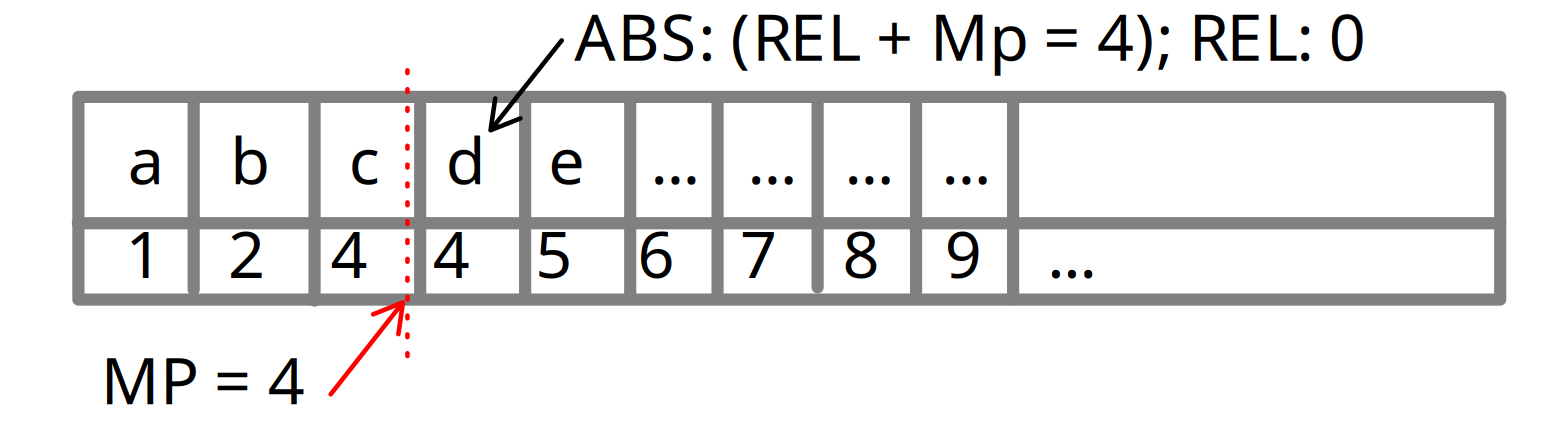
\includegraphics[width=\textwidth]{./vm_linmem_draft.png}
	\caption{\textcolor{red}{DRAFT:} Linear Memory of the rush VM}
	\label{fig:rush_vm_linmem}
\end{figure}

In order to get a deeper understanding of the addressing modes, a practical example can be considered.
The code in listing \ref{lst:rush_pointer_simple} displays a rush program in which a pointer to a variable is created.
First, the integer variable \texttt{num} is created.
In line 3, a pointer variable called \texttt{to\_num} is created by \emph{referencing} the \texttt{num} variable.

\TSListing[caption={Minimal Pointer Example in rush}, label={lst:rush_pointer_simple}, float=H]{listings/simple_pointer.rush}

In the rush VM, absolute addressing is only used for global variables and pointers.
Since a pointer specifies the address of another variable, its runtime value will be the absolute address of its target variable.
In the VM, the absolute address of a variable is calculated as soon as it is referenced using the \texttt{\&} operator.
For this purpose, the \texttt{reltoaddr} instruction exists.
This instruction calculates the absolute address of its operand and pushes the result onto the stack.
Here, the operand is the relative address of the variable to be referenced.
The listing \ref{lst:rush_pointer_simple_vm_instructions} shows the VM instructions generated from the rush program in listing \ref{lst:rush_pointer_simple}.

\TSListing[raw=true, caption={VM Instructions for the minimal Pointer Example}, label={lst:rush_pointer_simple_vm_instructions}, float=H]{listings/vm_instructions_simple_pointer.txt}

The first instruction \texttt{setmp} (\emph{set memory pointer}) increases the memory pointer by two.
This is because the \texttt{main} function contains two local variables whose space is to be allocated at the start of the function.
For instance, one might encounter \texttt{mp} being incremented by 0 since the corresponding function contains no local variables.
The next instruction \texttt{push} pushes the value 42 onto the stack.
In line 4, the \texttt{svari} (\emph{set variable immediate}) assigns the top value on stack to the specified relative address.
Here, 42 is popped off the stack since it is used by the \texttt{svari} instruction.
Next, the instruction stores the previously popped value at the relative address at the relative address 0 specified in the operand.
Now, the variable \texttt{num} with an initial value of 42 has been created.
Next, the \texttt{to\_num} variable is created by referencing the \texttt{num} variable.
In line 5, the \texttt{reltoaddr} (\emph{relative to address}) instruction is used to calculate the absolute memory address of the \texttt{num} variable.
This instruction calculates the absolute address of its operand at runtime using the algorithm described above.
Then, the instruction pushes the calculated address onto the stack so that it can be used by following instructions.
Here, the relative address 0 is used since the \texttt{svari} instruction has previously saved 42 at this location.
Therefore, the value of the variable \texttt{num} is saved at the relative address 0.
In line 6, the \texttt{svari} instruction is used again.
This time, it is used to save the value of the \texttt{to\_num} variable.
Since the absolute address of the referenced variable was previously calculated, it now exists on top of the stack.
Now, the instruction saves the absolute address of \texttt{num} at the relative address -1.
This is because the compiler targeting the VM assigns variables to higher relative addresses first.
The compiler then progresses into lower relative memory as more variables of the function are declared.
To summarize the above paragraph, this example uses relative addressing in order to declare local variables of a function.
However, absolute addressing is also used when variables are referenced in order to create pointers.
Therefore, each addressing mode serves a separate and important purpose.

\subsection{How the Virtual Machine Executes A rush Program}

By considering the minimal pointer example from above, we now have a rough idea how the VM might execute instructions.
In order to get a better understanding of how the rush VM works exactly, we will explain how it executes the program in listing \ref{lst:rush_vm_faster}.
For this, we should consider the instructions in Figure \ref{fig:tree_vs_vm} again.
The first instruction of the prelude function is \texttt{setmp}.
This instruction adjusts the memory pointer by the amount specified in the instruction's operand.
In this case however, the memory pointer remains unmodified since the operand of the instruction is 0.
Next, the \texttt{call 1} instruction calls the \texttt{main} function.
In order to understand how function calls work in this VM, we must consider the call stack of the rush VM.
Before the call-instruction, the caller pushes any call-arguments onto the stack so that they can be used as parameters by the callee.
Figure \ref{fig:rush_vm_call_stack} displays the state of the VMs call stack after the \texttt{call 1} instruction has been executed.
During execution of a call-instruction, the VM pushes a new stack frame onto its call stack.
Listing \ref{lst:call_frame_struct} shows how a call frame is implemented.

\TSListing[first line=26, last line=31, caption={Struct Definition of a \texttt{CallFrame}}, label={lst:call_frame_struct}, float=H]{deps/rush/crates/rush-interpreter-vm/src/vm.rs}

In this implementation, each call frame holds two important pieces of information.
In line 28 of listing \ref{lst:call_frame_struct}, the \texttt{ip} field is declared.
It specifies the \emph{instruction pointer} which holds the index of the current instruction.
Since the \texttt{call} instruction was interpreted previously, the instruction pointer of the new call frame is set to 0 as execution should continue at the first instruction of the called function.
The \texttt{fp} field is declared in line 30.
This field specifies the \emph{function pointer} which holds the index of the current function.

After the function call, \texttt{fp} is set to 1 since the main function is called and instruction should start at the first instruction of the main function.
Figure \ref{fig:rush_vm_call_stack} shows how the call stack of the VM looks like after the \texttt{call} instruction has been interpreted.
Function calls are managed in a stack in order to allow returning from functions.
If the VM encounters a \texttt{ret} (short for \emph{return}) instruction, it should leave the current function.
However, it should also know where to resume its fetch-decode-execute cycle.
For this, the VM just simply pops the top element from its call-stack.
Now, the top element on the stack contains the call-frame of the caller function.
In this call frame, \texttt{ip} still points to the \texttt{call} instruction which was responsible for calling the function.
Since \texttt{ip} is incremented automatically after most instructions, the VM resumes instruction execution at the first instruction after the call-instruction.
This way, function calls are implemented in a simple but robust manner.

% \begin{figure}[h]
% 	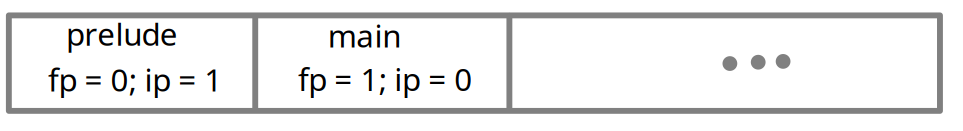
\includegraphics[width=\textwidth]{./vm_call_stack_draft.png}
% 	\caption{\textcolor{red}{DRAFT:} Call Stack of the rush VM}
% 	\label{fig:rush_vm_call_stack}
% \end{figure}

\begin{figure}
    \centering
    \begin{tikzpicture}
        \node[stack=3, rectangle split part align=center, text width=10ex, text centered, inner xsep=0]{
            \shortstack{prelude\\$fp=0$\\$ip=1$}
            \nodepart{two}{\shortstack{main\\$fp=1$\\$ip=0$}}
            \nodepart{three}{\ldots}
        };
    \end{tikzpicture}
	\caption{Call Stack of the rush VM}\label{fig:rush_vm_call_stack}
\end{figure}

Now that the call-instruction has been interpreted, the VM begins executing the first instruction of the main-function.
Since the main-function only calls the \texttt{rec} function with the argument 1000, there are no new concepts to consider in this function.
After the call instruction in line 7, the VM starts executing the instructions of the \texttt{rec} function.
At the beginning of the \texttt{rec} function, the memory pointer is incremented by 1.
This might seem erroneous since the \texttt{rec} function contains no visible variable declarations in its body.
However, this behavior is correct since function parameters count as variable declarations.
Since the function takes one parameter, the memory pointer is incremented by one cell.
Next, the instruction \texttt{svari} saves the value of the parameter which was previously pushed onto the stack at the relative address 0.
In line 12, the relative address of the memory cell containing the value of the parameter is pushed onto the stack.
It is then consumed by the \texttt{gvar} instruction in line 13.
At this point the top element on the stack contains an address-value referring to the target of the \texttt{gvar} instruction.
Therefore, the instruction first pops the top element from the stack.
In this case, the value of the popped element is the relative address 0.
Then, the instruction retrieves the value of the target variable and pushes it onto the stack.

In line 14, the constant value 0 is pushed onto the stack.
Next, the \texttt{eq} instruction pops two elements from the stack in order to test them for equality.
Then, the result of the comparison is pushed onto the stack as a boolean.
In this case, the instruction compares if the current value of \texttt{n} is equal to 0.
In line 16, the \texttt{jmpfalse} instruction is executed.
This instruction jumps to the specified instruction index if the value on top of the stack is \texttt{false}.
In this case, if the value on the stack is false, the parameter \texttt{n} was not equal to 0.
Now, the VM would jump to the instruction in line 19.
Here, the value of the parameter \texttt{n} is pushed onto the stack using the previously explained \texttt{push} and \texttt{gvar} instructions.
Now, the top item on the stack is the value of the parameter \texttt{n}.
In line 21, the \texttt{push} instruction pushes a constant 1 onto the stack.
Next, the \texttt{sub} instruction pops the first two elements from the stack in order to subtract their values from each other.
In this case, the instruction subtracts 1 from the value of \texttt{n} and pushes the result onto the stack.
Next, the \texttt{rec} calls itself recursively using a previously explained \texttt{call} instruction.
Since the call argument is the top element on the stack, the result of the subtraction is used as the argument of the recursive call.
Next, the function decrements the memory pointer in order to deallocate used memory using the \texttt{setmp} instruction in line 24.
At the end of a function, the memory pointer is always decremented by the amount it was incremented at the beginning of the function.
By deallocating the now unused memory, the compiler prevents the code from leaking memory at runtime.
Lastly, the \texttt{ret} instruction is used to return from the function.
Now we have considered what happens if the value of \texttt{n} was not equal to 0.

However, if the result of the comparison in line 15 is true, meaning that \texttt{n} is equal to 0, the \texttt{jmpfalse} instruction in line 16 does nothing.
In this case, the VM continues to the \texttt{push} instruction in line 17.
Here, the constant value 0 is pushed onto the stack.
Next, the VM interprets the \texttt{jmp} instruction in line 18.
Unlike \texttt{jmpfalse}, this instruction performs its jump without any condition.
In this case, the instruction jumps to the instruction at index 14 of the current function.
The instruction at index 14 is \texttt{setmp} in line 24.
Since functions also return values by placing them on top of the stack, the return-value would be 0 in this case.
Since we have covered what the instructions in the lines 24 and 25 do, we can summarize that the function returns the value 0 in this case.

Now that we have explained the semantic meaning of the instructions in Figure \ref{fig:tree_vs_vm}, we will explain how the fetch-decode-execute cycle works in the VM.
The code in listing \ref{lst:vm_run_meth} displays the \texttt{run} method of the rush VM.

\TSListing[first line=166, last line=177, caption={The \texttt{run} Method of the rush VM}, label={lst:vm_run_meth}, float=H]{deps/rush/crates/rush-interpreter-vm/src/vm.rs}

This method manages the entire fetch-decode-execute cycle of the VM.
It is immediately apparent that this method looks relatively simple considering that it plays such of a fundamental role in the VM.
Since the fetch-decode-execute cycle executes instructions repeatedly, the main construct in the function is a while-loop.
The condition of the loop checks that the current instruction pointer refers to a legal instruction inside the current function.
This way, the VM comes to a halt if it reaches the end of an instruction sequence.
In line 168, the next instruction to be interpreted is saved as the variable \texttt{instruction}.
This line represents the \emph{fetch} step since the next instruction is fetched from memory and placed in a spot where it can be used by the following steps.

In the body of the loop, the current instruction is executed using the \texttt{self.run\_instruction} method.
This method can return a runtime error, such as an integer-overflow error.
Furthermore, this method may return a integer representing the exit code of the program.
However, if the method returns none of these two possible types, the fetch-decode-execute cycle continues.
In this code however, one cannot observe the instruction pointer being incremented.
In order to answer the final question of how the current instruction is executed and the instruction pointer is incremented, we will now examine the code in listing \ref{lst:vm_run_instr_meth}.

\TSListing[first line=346, last line=359, caption={Parts of the \texttt{run\_instruction} Method of the rush VM}, label={lst:vm_run_instr_meth}, float=H]{deps/rush/crates/rush-interpreter-vm/src/vm.rs}

The code in listing \ref{lst:vm_run_instr_meth} displays the last part of the \texttt{run\_instruction} method.
This method mainly consists of an algorithm mathing the current instruction in order to execute specific code representing the instruction's semantic meaning.
In this example, the implementations of the \texttt{bitand} and \texttt{bitxor} instructions are visible.
Both instructions first pop two elements from the stack since they represent the operands of the underlying logical computation.
Then, a corresponding helper function is invoked on the left hand side operand.
The helper function then performs the actual computation of the logical operation.
Most of the infix-expressions are later executed in a similar way.
It is apparent that the execution of these instructions involves relatively little difficuilty.
After the instruction has been executed, the instruction pointer is finally incremented and nothing is returned.
For some special instructions, such as the jump-instructions, the instruction pointer should not be incremented since it would interfere with the jump.

\TSListing[first line=189, last line=192, caption={Execution of the \texttt{jmp} Instruction in the rush VM}, label={lst:vm_jmp_instr}, float=H]{deps/rush/crates/rush-interpreter-vm/src/vm.rs}

As seen in listing \ref{lst:vm_jmp_instr}, the \texttt{jmp} instruction only sets the instruction pointer to the target index specified in the instruction operand.
Then, the code returns from the method so that the instruction pointer is not incremented later.
This method represents both the \emph{decode} and \emph{execute} steps since it first matches (\emph{decode}) and then interprets (\emph{execute}) the current instruction.
Now that we have explained how some important parts of the rush VM work, we should now consider the compiler generating its input instructions.

\subsection{The Compiler Targeting the rush VM}

Since the rush VM interprets instructions directly, there must be a compiler translating the AST into these instructions.
For this purpose, we have implemented a compiler translating rush into instructions which can be understood by this VM.
Compared to the rush compiler targeting \emph{RISC-V},
implementation of this compiler has proven to be significantly simpler since the rush VM uses a stack-based design.
Since the VM's architecture was developed with the features of rush in mind,
the compiler sometimes requires suprisingly little effort for translating some AST-nodes. 
For instance, the compiler translates infix-expressions, such as $n + m$, into instructions using the \texttt{infix\_expr} method.
A part of this method is displayed in Listing \ref{lst:vm_compile_infix_expr}.

\TSListing[first line=538, last line=540, caption={Compilation of Infix-Expressions Targeting the VM}, label={lst:vm_compile_infix_expr}, float=H]{deps/rush/crates/rush-interpreter-vm/src/compiler.rs}

Here, the left hand side expression is compiled first.
Next, the right hand side is compiled too.
Finally, the appropiate arithmetic instruction is inserted.
The final instruction is generated by a helper function which converts an infix-operator into a matching instruction.
Most of the other compilers we have implemented for the rush project required significantly more code in order to implement the translation of infix-expressions.

\TSListing[first line=445, last line=450, caption={Compilation of Expressions Targeting the VM}, label={lst:vm_compile_expr}, float=H]{deps/rush/crates/rush-interpreter-vm/src/compiler.rs}

The code in Listing \ref{lst:vm_compile_expr} shows the top of the \texttt{expression} method in the VM compiler.
When we examine the method's signature, it becomes apparent that it only consumes an \texttt{AnalyzedExpresssion}.
However, the method does not return anything which represents the runtime value of the expression.
This is possible because the types of expression displayed in the listing are pushed onto the stack directly.
By pushing the values of atomic expressions onto the stack directly, most tree-traversing methods do not need to return values.
Due to this, short and elegant code like the one in listing \ref{lst:vm_compile_infix_expr} can be implemented.
In other compilers, the method responsible for compiling expressions usually returns the register which contains the value of the compiled expression at runtime.
This way, other parts of the compiled program can still use the runtime values of compiled expressions.

The rush VM includes a special instruction for the mathematical power operation (\texttt{**}).
Since many real architectures lack such a power instruction,
implementing a rush compiler targeting the VM has proven to be less demanding in this way.
On the opposite, many other rush compilers demanded implementation of special edge-cases in order to make compiling power-expressions feasible.
Furthermore, the VM also includes an \texttt{exit} instruction which terminates the fetch-decode-execute cycle instantly.
Here, the VM would come to a halt instantly, returning the top value on the stack as its exit code.
These examples showed how a carefully chosen target architecture simplies the implementation of its compiler by a great amount.

However, there is also one aspect of the VM which made implementation of the compiler targeting the VM more demanding than usual.
For instance, in most Assembly dialects, \emph{labels} can be used to allow jumps between blocks of code.
However, the VM intentionally does not support the use of such labels.
Since the VM would have to look up the exact instruction index of a label at runtime,
each jump targeting a label would involve some additional overhead.
This overhead is eliminated by the assembler during assembly of a program.
Since the assembler performs these lookups during translation,
the CPU does not have to deal with label lookups at runtime.
Like seen in the previous examples, jumping VM instruction require the exact index of the target instruction as their operands.
Therefore, the exact target index to which the instruction should jump must be known.
To illustrate this issue, we will consider how loops are implemented in the VM.
The rush code in Figure \ref{fig:vm_loops} presents a program containing a loop.
In the loop's body, the variable \texttt{n} is incremented by 1.
Next, the \texttt{break} keyword is used to terminate loop execution.
Therefore, the total amount of iterations is 1.

\noindent
\begin{figure}[h]
	\begin{minipage}{.5\textwidth}
		\centering
		\TSListing[frame=none]{listings/vm_basic_loop.rush}
	\end{minipage}%
	\begin{minipage}{.5\textwidth}
		\centering
		\TSListing[raw=true, frame=none]{listings/vm_basic_loop_instructions.txt}
	\end{minipage}
	\caption{How Loops are Interpreted by the VM}
	\label{fig:vm_loops}
\end{figure}

The rush VM instructions of the \texttt{main} function are displayed on the right side of Figure \ref{fig:vm_loops}.
Here, lines 2 and 3 are responsible for declaring the variable \texttt{n}.
The instructions in the lines 4-9 are used to increment the variable \texttt{n} by 1.
A new instruction which we have not covered so far is the \texttt{clone} instruction.
This instruction \emph{clones} the top item on the stack it without prior calls to \texttt{pop}.
Therefore, after the instruction has been executed, two idenical values exist on the top of the stack.
This instruction is only used in assign-expressions in order to duplicate the address value of the assignee variable.

After \texttt{n} is incremented, the instruction in line 10 jumps to the instruction index 11.
However, the last valid index is 10, it is represented by the \texttt{jmp 3} instruction.
If this occurs, the VM has no next instruction to fetch and therefore stops its fetch-decode-execute cycle.
Since this instruction jumps to a position outside the loop, it represents the \texttt{break} statement in line 5 of the source program.
The \texttt{jmp} instruction in line 11 is responsible for the repetition introduced by the loop.
This instruction jumps to the first instruction of the loop's body in line 4.
Therefore, the instructions inside the loop's body are executed repeatedly.
The difficuilty presented by this design is that the index of the jump's target instruction must be known before the target instruction is inserted.
The code in Listing \ref{lst:rush_vm_compiler_loop} displays a part of the method responsible for compiling loops for the rush VM.

\TSListing[first line=337, last line=343, caption={Implementation of Loops in the rush VM Compiler}, label={lst:rush_vm_compiler_loop}, float=H]{deps/rush/crates/rush-interpreter-vm/src/compiler.rs}

The statement in line 337 inserts the instruction responsible for jumping back to the start of the loop's body.
In line 340, the top loop is popped from the \texttt{loops} stack.
This stack is an internal field used by the compiler in order to save information about loops.
The top item on this stack always represents the loop currently traversed by the compiler.
Each loop saves two lists, each containing the indices of jump-instructions whose target index needs to be adjusted.
The first list contains the indices of jump-instructions generated by \texttt{break} statements
while the second lists saves instructions generated by \texttt{continue} statements.
For instance, if the compiler encounters a \texttt{break} statement, the code in listing \ref{lst:rush_vm_compiler_break} is executed.

\TSListing[first line=268, last line=273, caption={Compilation of \texttt{break} Statements in the rush VM Compiler}, label={lst:rush_vm_compiler_break}, float=H]{deps/rush/crates/rush-interpreter-vm/src/compiler.rs}

Here, the \texttt{pos} variable saves the index of the jump-instruction to be inserted.
In line 271, this index is then inserted into the list containing the placeholder indices of the current loop.
Lastly, the \texttt{jmp} instruction is inserted containing a placeholder target index.
Therefore, at the end of each loop's compilation, there will be a list containing the indices of instructions whose target indices need to be adjusted.
In line 342 of listing \ref{lst:rush_vm_compiler_loop}, the \texttt{self.fill\_blank\_jmps} method is used to set the target indices of the specified jump-instructions to \texttt{pos}.
We will omit the explaination of this method because it only iterates over the passed list of indices, replacing the target of the jump-instruction at the current index during the process.
Now, we have presented positive and negative aspects of writing a compiler targeting the rush VM.

As a conclusion, a VM is often a reasonable approach if an interpreted programming language is to be implemented.
The main advantages of a VM are increased speed and reduced memory usage at runtime.
The downsides include the need for a compiler targeting the VM, thus making its implementation more demanding. 


\chapter{Compiling to High-Level Targets}\label{chap:high_level_targets}
In the previous chapter, the implementation of a programming language using an interpreter has been explained.
However, another method of implementing a programming language is to create a compiler.
This chapter presents three different compilers for high-level targets, and one transpiler.

\section{How a Compiler Translates the AST}
\begin{wrapfigure}{r}{0.6\textwidth}
	\centering
	\begin{tikzpicture}[level distance=1cm, sibling distance=2.2cm]
        \node {Expression \encircle{5}}
        child {node {Expression \encircle{3}}
                child {node {Expression \encircle{1}}
						child {node {\Verb|Int(1)|}}}
				child {node {\Verb|Plus|}}
                child {node {Expression \encircle{2}}
						child {node {\Verb|Int(2)|}}}}
		child {node {\Verb|Lt|}}
        child {node {Expression \encircle{4}}
				child {node {\Verb|Int(4)|}}};
	\end{tikzpicture}
	\caption{Abstract syntax tree for `\texttt{1 + 2 < 4}'.}\label{fig:cmp_simple_tree}
\end{wrapfigure}

Often, a compiler traverses an AST generated by the analyzer in order to translate it to some sort of output.
For each AST node, the compiler usually calls a separate function or method which is specialized in translating this specific node type, similar to the tree-walking interpreter.
These individual methods return some sort of value representing the translated node.
Otherwise, each individual method may also insert generated instructions into an internal field of the compiler.
Here, the newly generated instructions are inserted into the output sequence.
In this case, each method also returns metadata about the previously compiled node.
For instance, this data may include the register or memory location of a previously compiled expression, so that other AST nodes can refer to it later.
In transpilers, i.e., compilers translating one high-level language into another one, each node-specific method returns another tree node representing code of the output language.

Figure~\ref{fig:cmp_simple_tree} displays a simplified syntax tree of the rush expression `\texttt{1 + 2 < 4}'.
The encircled number after each expression represents the order in which most compilers would traverse this tree.
Compilation of the expression starts at the root node of the tree.
Here, most compilers will begin translation by first compiling the child nodes using \emph{post-order} traversal.
Post-order traversal is frequently used because the compilation of a node often depends on the output of its child nodes.
In this example, translation of the root comparison expression depends on the information returned by compiling its left- and right-hand sides.
Therefore, the compiler first considers the node `Expression~\encircle{3}' which represents the infix-expression \qVerb{1 + 2}.
However, due to post-order traversal, this node is not actually processed since the compiler skips straight to its child nodes.
Therefore, the left child `Expression~\encircle{1}' is traversed as the very first node.
Next, its sibling node `Expression~\encircle{2}' is traversed.
Since post-order traversal involves considering a root node after the traversal of its children, `Expression~\encircle{3}' is traversed after \encircle{1} and \encircle{2} have been considered.
Here, the compiler considers the operator of the expression in order to generate the appropriate output instruction.
Therefore, the instruction responsible for the addition is inserted after `Expression~\encircle{3}' has been traversed.
Since it and its children are now completed, and its output instruction has been inserted, the compiler now considers the right-hand side of the comparison.
Here, the node `Expression~\encircle{4}' only consists of the integer literal `4'.
Now, all child nodes of `Expression~\encircle{5}' have been traversed, thus the compiler now considers this node itself.
Here, the compiler also inserts the appropriate instruction, that is, a less-than comparison between integers.
Since the compiler must be aware of the operands of the instruction, each method involved in the tree traversal returns an entity describing the location of the runtime value of its previously compiled node.
For instance, if the target architecture uses registers, every method translating an expression must return the register or memory location containing the value of the expression at runtime.
By returning information like this, a node will have information about its children after they have been traversed.
It might rely on the values returned by its children, therefore it is traversed at last, thus creating the demand for post-order traversal.

\Lirsting[raw=true, caption={Simple pseudo-instructions for a fictional architecture.}, label={lst:cmp_simple_instructions}, wrap=l, wrap width={.32\textwidth}]{listings/simple_compiler_instructions.txt}

Listing~\ref{lst:cmp_simple_instructions} displays a sequence of instructions for a fictional architecture.
This sequence could have been generated from the previously discussed tree in Figure~\ref{fig:cmp_simple_tree}.
It is apparent that the order of instructions matches the order in which the tree was traversed.
The instructions in lines~1 and 2 represent the tree-nodes `Expression~\encircle{1}' and `Expression~\encircle{2}' respectively.
Here, the value `1' is assigned to a register named `\texttt{r0}' while the value `2' is assigned to the register `\texttt{r1}'.
The \qVerb{add} instruction in line~3 appears after the instructions in lines~1 and 2 since their tree nodes were traversed first.
Furthermore, the instruction uses the registers \qVerb{r0} and \qVerb{r1} as its operands and therefore depends on them containing a value.
Therefore, the \qVerb{add} instruction can use the registers returned by compiling its child nodes as its operands.
Next, the integer `4' is assigned to the register `\texttt{r3}'.
Lastly, the comparison instruction \qVerb{lt} uses the result of the addition and the register containing `4' as its operands.
Here, it is apparent that the instruction generated by the node which was traversed at last is also inserted at the end.

Therefore, using post-order traversal in order to generate output instructions targeting a register-based architecture is often required.
This example illustrates how a simple compiler might operate.
However, a similar algorithm is often found in even the most complex compilers.

\subsection{The Compiler Targeting the rush VM}\label{sec:vm_compiler}

Since the rush VM interprets instructions directly, there must be a compiler targeting its architecture.
For this purpose, we have implemented a compiler translating rush source code into instructions which can be understood by the VM\@.
Since the VM's architecture was developed with the features of rush in mind,
the compiler sometimes requires surprisingly little effort for translating certain AST-nodes.
For instance, the compiler translates infix-expressions, such as `\texttt{n + m}', into instructions using the \qVerb{infix_expr} method.
This method is displayed in Listing~\ref{lst:vm_compile_infix_expr}.

\Lirsting[ranges={522-524,536-543}, caption={Compilation of infix-expressions targeting the VM.}, label={lst:vm_compile_infix_expr}, float=h]{deps/rush/crates/rush-interpreter-vm/src/compiler.rs}

This method differentiates between the `\texttt{Or}' / `\texttt{And}' operators and other possible operators since the former require some extra code to be emitted.
However, due to simplicity, the focus only lies on the compilation of the latter, meaning any other type of infix-expression.
In line 538, the left-hand side expression is compiled first.
In the next line, the right-hand side is compiled too.
Finally, in line 540, the matching instruction representing the infix-operator is inserted.
The final instruction is generated by a helper function which converts an infix-operator into a matching instruction.
It is to be mentioned that most of the other rush compilers required significantly more code in order to implement the translation of infix-expressions.
The reason for the simplicity of this implementation is the fact that the rush VM implements one instruction for each infix-operator.
Since this VM implements all features of the source language, complex hacks for implementing some operations are not required and thereby simplify the compiler's implementation.

\Lirsting[ranges={445-447,457-461}, caption={Compilation of expressions targeting the VM.}, label={lst:vm_compile_expr}, float=h]{deps/rush/crates/rush-interpreter-vm/src/compiler.rs}

The code in Listing~\ref{lst:vm_compile_expr} shows parts of the `\texttt{expression}' method of the rush VM compiler.
When we examine the method's signature, it becomes apparent that it consumes an \qVerb{AnalyzedExpresssion}.
However, the method does not return anything which represents the runtime value of the expression.
This is possible because the results of the expressions displayed in the snipped are pushed onto the stack directly.
In line 447, the code for translating a constant integer expression can be seen.
Here, a push instruction using the constant int value as its operand is used.
By pushing the values of expressions onto the stack directly, most tree traversing methods do not need to return values.
Due to this, short and elegant code like the one in Listing~\ref{lst:vm_compile_infix_expr} can be implemented.
In other compilers, the method responsible for compiling expressions would usually return the register which contains the value of the compiled expression at runtime.
Due to the values being saved on the VM's stack, other parts of the compiled program can still use the runtime values of compiled expressions.
In line 457, the method for compiling call-expressions would be invoked.
Similar to the `\texttt{expression}' method in the analyzer, this method also dispatches the traversal of more complex expressions to specialized methods in order to keep this method simple.

Another reason for the compiler's simplicity regarding infix-expressions is that the rush VM includes a special instruction for the mathematical power operation.
In rush, the expression `\texttt{n ** m}' can be used to denote following mathematical term: $n^m$.
Since many real architectures lack such a power instruction, most other rush compilers demanded implementation of special edge-cases in order to make compiling power-expressions feasible.
On the opposite, implementing a rush compiler targeting the VM has proven to be less demanding since the VM supports a power-instruction.
Furthermore, the VM also includes an `\texttt{exit}' instruction which terminates the fetch-decode-execute cycle instantly.
These examples showed how a carefully chosen target architecture simplifies the implementation of its compiler by a great deal.

However, there is also one aspect of the VM which made implementation of the compiler targeting the VM more demanding than usual.
For instance, in most Assembly dialects, \emph{labels} can be used to allow jumps between blocks of code.
However, the VM intentionally does not support the use of such labels.
Since the VM would have to look up the exact instruction index of a label at runtime,
each jump targeting a label would involve some additional overhead.
This overhead is eliminated by the assembler during assembly of a program.
Since the assembler performs these lookups during translation,
the CPU does not have to deal with label lookups at runtime.
Like seen in the previous examples, jumping VM instruction require the exact index of the target instruction as their operands.
Therefore, the exact target index to which the instruction should jump must be known.
To illustrate this issue, we will consider how loops are implemented in the VM\@.
The rush code in Figure~\ref{fig:vm_loops} presents a program containing a loop.
In the loop's body, the variable `\texttt{n}' is incremented by 1.
Next, the `\texttt{break}' keyword is used to terminate loop execution.
Therefore, the total amount of iterations is 1.

\noindent
\begin{figure}[h]
	\begin{minipage}{.5\textwidth}
		\centering
		\Lirsting[fancyvrb={frame=none}]{listings/vm_basic_loop.rush}
	\end{minipage}%
	\hfill
	\begin{minipage}{.5\textwidth}
		\centering
		\Lirsting[raw=true, fancyvrb={frame=none}]{listings/vm_basic_loop_instructions.txt}
	\end{minipage}
	\caption{Representation of loops in the VM.}\label{fig:vm_loops}
\end{figure}

The rush VM instructions of the `\texttt{main}' function are displayed on the right side of Figure~\ref{fig:vm_loops}.
Here, lines 2 and 3 are responsible for declaring a variable named `\texttt{n}'.
The instructions in the lines 4--9 are used to increment `\texttt{n}' by 1.
A new instruction which we have not covered so far is the `\texttt{clone}' instruction.
This instruction \emph{clones} the top item on the stack it without prior calls to `\texttt{pop}'.
Therefore, after the instruction has been executed, two identical values exist on the top of the stack.
This instruction is only used in assign-expressions in order to duplicate the address value of the assignee variable.

After `\texttt{n}' was incremented, the instruction in line 10 jumps to the instruction index 11.
However, the last valid index is 10, it is represented by the `\texttt{jmp 3}' instruction in line 11.
If this jump is executed, the VM has no next instruction to fetch and therefore stops its fetch-decode-execute cycle.
Since this instruction jumps to a position outside the loop, it represents the \qVerb{break} statement in line 5 of the source program.
The `\texttt{jmp}' instruction in line 11 is responsible for the repetition introduced by the loop.
This instruction jumps to the first instruction of the loop's body in line 4.
Therefore, the instructions inside the loop's body are executed repeatedly.
The difficulty presented by this design is that the index of the jump's target instruction must be known before the target instruction is inserted.
The code in Listing~\ref{lst:rush_vm_compiler_loop} displays a part of the method responsible for compiling loops for the rush VM\@.

\Lirsting[ranges={320-323,331-331,337-344}, caption={Implementation of loops in the rush VM compiler.}, label={lst:rush_vm_compiler_loop}, float=h]{deps/rush/crates/rush-interpreter-vm/src/compiler.rs}

In line 331, the loop's body is compiled and instructions generated during this process are inserted into the output sequence.
The next statement in line 337 inserts an instruction responsible for jumping back to the start of the loop's body.
The variable `\texttt{loop\_head\_pos}' was previously defined and species the index of the first instruction of the loop's body.
Therefore, this inserted instruction performs continuous jumps, thereby introducing the repetition for which the loop is desired.

In line 340, the top loop is popped from the `\texttt{loops}' stack.
In line 322, this loop was previously pushed onto the identical stack.
This stack is an internal field used by the compiler in order to save information about loops.
The top item on this stack always represents the loop currently traversed by the compiler.
Each loop item saves two lists, each containing the indices of jump-instructions whose target index needs to be adjusted.
The first list contains the indices of jump-instructions generated by `\texttt{break}' statements which were encountered during traversal of the loop's body.
The second list saves the indices of jump-instructions emitted by `\texttt{continue}' statements inside the loop's body.
For instance, if the compiler encounters a `\texttt{break}' statement, the code in Listing~\ref{lst:rush_vm_compiler_break} is executed.

\Lirsting[ranges={253-253,268-273,287-288}, caption={Compilation of \qVerb{break} statements in the rush VM compiler.}, label={lst:rush_vm_compiler_break}, float=h]{deps/rush/crates/rush-interpreter-vm/src/compiler.rs}

Here, the `\texttt{pos}' variable saves the index of the jump-instruction to be inserted.
In line 271, this index is then inserted into the list containing the placeholder indices of the current loop.
Lastly, a `\texttt{jmp}' instruction is inserted containing a placeholder target index.
Therefore, at the end of the compilation of a loop's body, there will be a list containing the indices of instructions whose target indices need to be adjusted.
In line 342 of Listing~\ref{lst:rush_vm_compiler_loop}, the `\texttt{self.fill\_blank\_jmps}' method is used to set the target indices of the specified jump-instructions to `\texttt{pos}'.
We will omit the explanation of this method because it only iterates over the passed list of indices, replacing the target of the jump-instruction at the current index during the process.

As a conclusion, design, and implementation of the compiler targeting the rush VM has presented itself as a reasonable task.
Altering the target architecture to mitigate difficulties which occurred during the implementation of the compiler was often extremely helpful.
Therefore, compared to the rush compiler targeting \riscv{},
implementation of this compiler was significantly simpler.
Furthermore, the rush VM uses a stack-based design which made implementing its compiler less demanding as well.

\section{Compilation to WebAssembly}

\begin{enumerate}
	\item what is WASM and why
	\item modules
	      \begin{itemize}
		      \item binary and text format (sections, leb128)
		      \item globals, functions, imports, exports, \ldots
		      \item uncommon to target binary format
	      \end{itemize}
	\item WASI
	\item basic implementation
	      \begin{itemize}
		      \item leb128
		      \item sections
		      \item \Verb{self.function_body}
	      \end{itemize}
	\item example program
\end{enumerate}

The first `external' compilation target presented here is \emph{WebAssembly}, or \emph{WASM} for short.
\TODO{research origins and goals of WASM and explain them here}
Unlike the name implies, WebAssembly is not only used in web applications.
By itself, it is only a specification that can be implemented by runtimes in any context.
Most modern browsers include such a WebAssembly runtime, but there are also standalone ones, for example \emph{wasmtime} and \emph{wasmer}.

\subsection{WebAssembly Modules}

Every valid WebAssembly file must contain exactly one module.
\TODO{confirm}
The WebAssembly specification defines two different representations for these modules.
First, there is a human-readable text representation, called \emph{WAT}\footnote{WebAssembly Text}, closely resembling S-Expressions\footnote{\TODO{what are S-Expressions}}.
This is comparable to assembly languages for CPU architectures and is the typical target for compilers.
Secondly, WebAssembly modules can also be represented using its binary format, which is optimized for size and comparable to the final binary files produced by assemblers.
Most often these binary modules are constructed from a text module by using a tool such as \emph{wat2wasm} from the \emph{WebAssembly Binary Toolkit (WABT)}.
However, the rush WebAssembly compiler instead opts to target the binary format directly, highlighting a few reasons for why most compilers should not do this.
Listing~\ref{lst:wat_demo_wat} and Listing~\ref{lst:wat_demo_hex} on page~\pageref{lst:wat_demo_wat} show the same basic WebAssembly module once as WAT and once as a commented hex dump of the same module in its binary representation as produced by \url{https://webassembly.github.io/wabt/demo/wat2wasm/}.

\Lirsting[float=p, label={lst:wat_demo_wat}, caption={Simple WebAssembly Module in Text Representation}]{listings/wat_demo.wat}
\Lirsting[float=p, label={lst:wat_demo_hex}, caption={Simple WebAssembly Module in Binary Representation}]{listings/wat_demo.hexdump}

Focusing on the text representation first, the shown module contains one function that takes two \qVerb{i32}s as parameters and returns a single \qVerb{i32}.
An \qVerb{i32} in WebAssembly represents an uninterpreted 32-Bit integer, that is, it is not clear whether the integer is signed or unsigned from the type itself.
Instead, values of this type can be interpreted as either signed or unsigned by different instructions.
For instance, the instruction \qVerb{i32.eq}, which checks for equality between two \qVerb{i32} values, behaves the same no matter the integer's signedness.
In contrast, \qVerb{i32.lt_s} and \qVerb{i32.lt_u} are two instructions both querying whether one \qVerb{i32} is less than another, once for signed and once for unsigned integers as denoted by the suffix.

The mentioned function is exported by the module under the name `addTwo' to make it accessible from outside.
What exactly `outside' is depends on the context the module is run in.
WebAssembly is \emph{stack based} and has one primary stack each instruction operates on.
The first two instructions of the `addTwo' function retrieve the local variable of the given index and push its value to the stack.
`Locals' in WebAssembly are simple values separate from the main stack.
Function parameters are always the first locals, but additional ones can be added, too.
After the two instructions ran, the stack now contains the values of the two function parameters.
They are then added by \qVerb{i32.add} which pops the top two elements off the stack and pushes the sum back on.
The return value implicitly is always what remains on the stack at the end of a function body.

Now focusing on the hex dump of the same module in binary in Listing~\ref{lst:wat_demo_hex}.
A WebAssembly binary file always starts with the four bytes \qVerb{00 61 73 6d} called the \emph{WASM binary magic} and representing a zero byte followed by the string `asm' using ASCII representation.
This is used by other programs to easily identify binary files as WebAssembly modules.
Following that is the version of the binary format, stored as a 32-Bit integer in Little-Endian\footnote{Little-Endian starts with the least significant byte first, whereas Big-Endian starts with the most significant byte}.
At the time of writing it is always `1'.

The binary module is then split into different sections each containing one kind of information about the whole.
Empty sections can be omitted.
Each section begins with its identifier, followed by the section size in bytes.
Most sections contain one vector of relevant data, and vectors always start with the count of elements they contain, and continue with the elements themselves.
The first section present here is the `Type' section.
It declares different types used by the module, most importantly, the function signatures.
The `Function' section then contains the number of functions of the current module and simply references to the `Type' section for each function's signature.
The module's exports are declared in the `Export' section.
Finally, the `Code' section contains the actual instructions for each function.
It is again stored as a vector, containing function bodies for all functions defined in the `Function' section in the same order.
Each function body begins with its size in bytes, continues with the instructions, and ended by an \qVerb{end} instruction represented by a \qVerb{0b} byte.

The `wat2wasm' tool used here additionally adds a custom `name' section.
Custom sections always have the ID `0' and must provide a custom name using ASCII.
This `name' section has its own specification separate from the main module specification, and is used to provide names for functions and variables that can then be used by development tools like `wasm2wat'.

Apart from exporting, WebAssembly modules can also import functions from outside.
Only the name and type signature must be provided and the WebAssembly runtime will then have to provide an implementation when running.
Furthermore, WebAssembly does not only have local variables, but also global ones, accessible from every function.
These must be initialized with some constant value and can either be mutable or immutable.

One may already have noticed that except for the version number at the start, all sizes, indices, lengths, and so on, have been stored using just a single byte.
But, this is not because those can only reach a maximum of 255, but instead WebAssembly uses the LEB128 encoding for integer literals in binary modules.
It is a space efficient way to store integers by only ever needing as many bytes as necessary for a number.
The encoding details are not explained here however, and our implementation for the rush compiler simply uses a pre-existing crate\footnote{A crate is a library in Rust terms} called `leb128'.

\subsection{The WebAssembly System Interface}

Since WebAssembly itself does not provide any guarantees about the runtime environment, it does not provide ways to interact with the environment, except, of course, for module imports and exports.
That is why an additional specification called the \emph{WebAssembly System Interface}, short \emph{WASI}, was created for WebAssembly modules that wish to communicate with an operating system.
Any runtime supporting WASI must provide a set of functions comparable to \emph{system calls} on Linux or Windows.
These can then be imported from a WebAssembly module to do things like writing to a console and exiting with a specific exit code.
Both wasmtime and wasmer implement the WASI interface.

A WebAssembly module making use of WASI must export one function under the name \qVerb{_start} that acts as the entry point.
The rush WebAssembly compiler only ever imports WASI's \qVerb{proc_exit} function which takes one 32-Bit integer as an argument and terminates execution with the given code.

\TODO{anything else to explain/mention here?}

\subsection{Implementation}

\Lirsting[ranges={324-328}, path prefix={deps/rush}, wrap=R, fancyvrb={numbers=right}, label={lst:wasm_instructions}, caption={Definition of Instruction Opcodes}]{deps/rush/crates/rush-compiler-wasm/src/instructions.rs}

The rush WebAssembly compiler directly targets the binary format.
This complicates compilation in a few ways, but removes the need for any external dependencies.
First, public constants are defined for all instructions and all types in separate files.
Listing~\ref{lst:wasm_instructions} shows an extract.

The \qVerb{Compiler} struct has a lot of fields for various purposes.
Only a few are shown in Listing~\ref{lst:wasm_compiler} and explained here.
To begin, a few fields regarding the currently compiled function are defined.
The \qVerb{function_body} contains the bytes with instructions for this function, and \qVerb{locals} stores which locals the function has along with their types.
In the binary format the locals are stored as a WebAssembly vector, that is, it starts with the number of locals, followed by each local.
Since the compiler cannot know the count of local variables beforehand, it stores them as a vector of byte vectors first.
This way, in the end it can first append the vector's length to the final output and then concatenate the contents.

\Lirsting[ranges={11-15, 26-31, 37-39, 58-58}, path prefix={deps/rush}, float=h, label={lst:wasm_compiler}, caption={\qVerb{Compiler} Struct Definition of the WebAssembly Compiler}]{deps/rush/crates/rush-compiler-wasm/src/compiler.rs}

\TODO{explain other shown fields}

\subsection{Example}

\TODO{example}

\section{Using LLVM for Code Generation}

LLVM is a software project intended to simplify the construction of a compiler generating highly-performant output programs.
It originally started as a research project by \emph{Chris Lattner} for his master's thesis at the University of Illinois at Urbana-Champaign~\cite{Lattner:MSThesis02}.
Since then, the project has been widely adopted by the open source community.
In 2012, the project was rewarded the \emph{ACM Software System Award}, a prestigious recognition of significant software which contributed to science.
From the point when popularity of the framework grew, it was renamed from \emph{Low Level Virtual Machine} to the acronym it is known by today.
Today, it can be recognized as one of the largest open source projects~\cite[preface]{Cardoso_Lopes2014-jt}.
Among many other projects, the Rust programming language depends on the LLVM compiler in order to generate its target-specific code~\cite[p.~373]{McNamara2021-hz}.
Furthermore, the \emph{Clang} C / C++ compiler uses LLVM as its code generating backend~\cite[preface]{Hsu2021-ez}.
Therefore, production ready compilers for popular programming languages have been implemented using the LLVM framework.
Besides open-source projects, many companies have also incorporated LLVM in their commercial software.
For instance, since 2005, Apple has started incorporating LLVM into some of its products~\cite[pp.~11-15]{Fandrey}.
A recent example of software developed by Apple which uses LLVM is the \emph{Swift} programming language which is mainly used for developing IOS apps~\cite[preface]{Hsu2021-ez}.

\subsection{The Role of LLVM in a Compiler}

In a compiler system, LLVM is responsible for generating target-specific code and performing optimizations.
The framework is known for performing very effective optimizations during code generation so that the translated program runs faster at runtime and uses less memory.
In order to use LLVM, the system provides and API which is usable by earlier steps of compilation.
Typically, a compiler frontend only analyzes the source program to create an AST.
Next, a separate step of compilation invokes the LLVM framework which carries on from this point\@.
This component traverses the AST and uses the API of LLVM in order to construct an intermediate representation of the program.
This way, the framework will be able to understand the semantic meaning of the program.
Next, LLVM compiles the input program to an output which is specific to an arbitrary target architecture.
As of today, LLVM features many target architectures so that a compiler designer does not have to worry about portability of the output program~\cite[preface]{Hsu2021-ez}.
Listing~\ref{fig:compilation_steps_llvm} shows how LLVM integrates into the previously discussed steps of compilation.
Therefore, the framework represents the \emph{back end} component of a compiler.

\begin{figure}[h]
	\centering
	\begin{tikzpicture}[node distance=3mm and 1cm, inner sep=3mm]
		\node (syntactic_analysis_text) [inner sep=0] {syntactical analysis};
		\node (lexical_analysis) [rec, below=of syntactic_analysis_text] {lexical analysis};
		\node (syntactic_analysis) [rec, fit={(syntactic_analysis_text) (lexical_analysis)}] {};

		\node (semantic_analysis) [rec, align=center, right=of syntactic_analysis] {semantic\\analysis};
		\draw [arrow] (syntactic_analysis) -- (semantic_analysis);

		\node (ir_generation) [rec, align=center, right=of semantic_analysis] {LLVM IR\\generation};
		\draw [arrow] (semantic_analysis) -- (ir_generation);

		\node (llvm) [rec, align=center, fill=gray!20, right=of ir_generation] {LLVM\\backend};
		\draw [arrow] (ir_generation) -- (llvm);
	\end{tikzpicture}
	\caption{Steps of Compilation When Using LLVM}\label{fig:compilation_steps_llvm}
\end{figure}

The updated Figure~\ref{fig:compilation_steps_llvm} now includes two new steps: \enquote{LLVM IR generation} and \enquote{LLVM backend}.
The first step generates the target-independent input used by the second step to generate target-specific code.
This step traverses the AST in order to generate a semantically equivalent program formulated using LLVM's intermediate representation.
A compiler writer must only implement the first three steps of this figure as the last step is represented by the framework itself.

\subsection{The LLVM Intermediate Representation}

The LLVM intermediate representation (\emph{IR}) represents the source program in a low-level manner.
However, even though this IR is low-level, it is still target-independent.
Furthermore, the IR also contains detailed type information which is usually uncommon for low-level representations of a program.
Therefore, high-level type information is preserved while the benefits of a low-level representation are introduced.
This allows LLVM to perform significant more aggressive optimizations compared to other compiler solutions or frameworks.
Therefore, programs compiled using LLVM as the backend will often run significantly faster due to the many aggressive optimizations introduced by the framework.

LLVM provides many APIs for interacting with the IR in memory.
This way, it can be created by a frontend without the need for a separate file containing the IR.
If the file containing the IR is written and read by the individual parts of the compiler,
the same performance issues introduced by multipass compilation would emerge.
Therefore, LLVM provides official APIs for the \emph{C++} and \emph{C} programming languages.
However, there are many unofficial bindings, such as for Rust, Go, or Python.
For instance, a compiler frontend written in Rust can leverage LLVM, although the system is written in C++.
Since LLVM must be able to perform complex program analysis before it can optimize a program,
its IR introduces many rules and constraints.
For instance, a program formulated using the IR should always obey the following hierarchy:

\begin{itemize}
	\item The top most hierarchical structure is the so-called \emph{module}.
	      It represents the current file being compiled.
	\item Each module contains several \emph{functions}.
	      Often, each function in the source program is represented using a function in the IR\@.
	\item Each function contains several \emph{basic blocks}.
	      A basic block contains a sequence of instructions.
	      Blocks should always be terminated using a jump, return, or unreachable instruction.
	      However, a basic block must never be terminated twice.
	\item Each basic block contains a sequence of \emph{instructions}.
	      Each instruction holds a semantic meaning and represents a part of the source program.
	      For instance, LLVM provides instructions for integer addition or function calls.
\end{itemize}~\cite[p.~211-213]{Hsu2021-ez}.

The IR provides a low-level enough representation in order to allow optimizations in the early stages of compilation.
However, due to the high-level type information contained in the IR,
LLVM is able to perform many aggressive optimizations on the IR during later stages of compilation.
This way, the framework can communicate a lot of information to the linker which can then use this information for \emph{link-time} optimizations.
The virtual instruction set of LLVM is therefore designed as a low-level representation with high-level type information.
This instruction set describes a virtual architecture which is able to represent an abstraction for most of the common types of processors.
Although it is low-level, the IR avoids machine specific constraints like registers or calling conventions.
Instead, the virtual architecture provides an infinite set of virtual registers which can hold the value of primitives like integers, booleans, floating-point numbers, and pointers.
All registers in the IR use the \emph{SSA}\footnote{Short for \enquote{static single assignment}, widely used in optimizing compilers} form in order to allow more optimizations.
In order to enforce the correctness of the type information included in the IR, the operands of each instruction all obey LLVM's type rules.
Therefore, LLVM only processes a program which contains valid type information~\cite[p.~14-17]{Lattner:MSThesis02}.

In order to understand how a program can be formulated using the LLVM IR, we consider the rush program for calculating Fibonacci numbers again.
For reference, the rush program used in this example can be found in Listing~\ref{lst:rush_fib} on page~\pageref{lst:rush_fib}.
The code in Listing~\ref{lst:llvm_fib} displays the identical rush program formulated in LLVM IR\@.
The IR was generated by the LLVM targeting rush compiler\footnote{Generated in Git commit \rushCommit{}, automatically built with this document}.
This compiler is presented in a later chapter since right now, only its output is of relevance.
The IR displayed in this listing shows a module named \qVerb{main}.

\Lirsting[ranges={1-30}, caption={LLVM IR Representation of the Program in Listing~\ref{lst:rush_fib}}, label={lst:llvm_fib}, float=h]{listings/generated/fib.ll}

In the lines 5 and 23, two functions are defined using the \qVerb{declare} keyword.
It is apparent that the functions in the LLVM module represent the functions from the source rush program.
The function's name in the IR matches the name in the source file as it increases readability of the program.
When examining the signature of the \qVerb{fib} function in line 5 of the IR,
it becomes apparent that the function returns a runtime value of the type \qVerb{i64}.
In rush, the \qVerb{int} type represents a 64-bit signed number.
Therefore, the \qVerb{i64} LLVM type represents the rush \qVerb{int} type.
Furthermore, we can observe that the function takes a parameter named \qVerb{\%0} of the type \qVerb{i64}.
It represents the `\texttt{n}' parameter in the rush source program.

In line 6, the start of the \qVerb{entry} block of the \qVerb{fib} function is declared using the block's name followed by a colon.
Since LLVM can perform more optimizations on variables if they are declared in the \qVerb{entry} block of a function,
the rush compiler uses the \qVerb{entry} block solely for variable declarations.
In line 7, the \qVerb{icmp slt}\footnote{Short for \enquote{integer compare (signed less than)}} is used in order to compare the runtime value of the parameter `\texttt{\%0}' to a constant 2.
The boolean result is then saved in a virtual register named `\texttt{\%i\_lt}'.
Since LLVM's virtual registers may have arbitrary names,
the rush compiler uses names which will make reading of the generated IR easier.
In line 8, the block is terminated using the \qVerb{br}\footnote{Short for \enquote{branch}} instruction.
The instruction will only jump under the condition that the value of `\texttt{\%i\_lt}' is true.
%Here, we can see that LLVM instructions are able to operand on different type of operands depending on what the instruction should do.
Here, the \qVerb{merge} and the \qVerb{else} labels are used as operands of the branch-instruction.
Conditional jumps in LLVM always require an alternative jump to perform if the condition is false at runtime.
Due to constraints introduced by its internal optimizations, LLVM only allows jumps to target blocks contained in the same function.
Therefore, two labels of blocks in the current function are used as the operands of this instruction.
As the names \qVerb{merge} and \qVerb{else} suggest, this branch-instruction presents the essential part of the if-expression in the source program.
If the condition was true at runtime, the instruction would jump to the \qVerb{merge} block in line 10.
What might seem odd is that there is no \qVerb{if} block.
In fact, the rush compiler has even compiled this block into LLVM IR\@.
However, since that block only jumped to the \qVerb{merge} block, LLVM's optimizations removed it entirely.

In line 11, of the \qVerb{merge} block, the \qVerb{phi} instruction is used.
These so called $\phi$-nodes are necessary due to the SSA form used in the IR\@.
In short, a \emph{phi-node} produces a different value depending on the basic block where control came from.
Since the if-construct is an expression in rush, LLVM must know if the result of the \qVerb{entry} or the \qVerb{else} branch is to be used as the result of the entire if-expression.
As a solution to this problem, these phi-nodes associate a value to an origin branch.
In this example, the phi-node yields the value of the parameter `\texttt{\%0}' (\qVerb{n}) if control came from the \qVerb{entry} block.
In the source program, \qVerb{n} should be returned without modification if it is less than 2.
Therefore, the runtime result of the phi-node is `\texttt{\%0}' if it is less than 2 at runtime.
Otherwise, if control came from the \qVerb{else} block, the phi-node's result is taken from the virtual register `\texttt{\%i\_sum3}'.
However, we have not covered where this virtual register is declared.
For this, we consider the instructions in the \qVerb{else} block, starting in line 15 with the `\texttt{add}' instruction.
In this case, the instruction subtracts 2 from the parameter `\texttt{\%0}' and saves the result in `\texttt{\%i\_sum}'.
However, an addition instruction using a negative operand is used since LLVM's optimization decided that this instruction is likely beneficial.
This is done in order to create the argument value for the first recursive call to \qVerb{fib}.
Next, the \qVerb{call} instruction is used in order to perform the recursive call.
Here, the `\texttt{\%i\_sum}' register is used as an argument to the call-instruction.
The return value of the function call is saved in the `\texttt{\%ret\_fib}' register.
The same behavior is used in order to call \qVerb{fib(n - 1)}.
However, in that case, 1 is subtracted from the parameter and saved in `\texttt{\%i\_sum1}'.

Next, the \qVerb{add} instruction in line 19 is used in order to calculate the sum of the return values of the recursive calls
This sum is then saved in the virtual register `\texttt{\%i\_sum3}'.
Therefore, this register is used in the phi-node in line 11 so that the result of the recursive calls is used as the result of the if-expression.
Next, the \qVerb{br} instruction jumps to the `\texttt{merge}' block.
However, this jump happens unconditionally since the instruction does not consider a condition and only has one target label.
After the jump to the \qVerb{merge} block, the previously explained $\phi$-node is encountered.
Finally, the \qVerb{ret} instruction in line 12 is used in order to use the result of the if-expression as the return-value of the function.
Since the \qVerb{main} function does not introduce any new concepts, we will omit detailed explanation of its contents.
However, in line 27, the \qVerb{unreachable} instruction is used in order to state that it is never executed.
This is necessary because LLVM requires that every basic block is terminated at its end.
The `\texttt{exit}' function terminates the program using a system call and therefore terminates the basic block.
However, LLVM does not regard call-instructions as diverging and therefore disallows the call to \qVerb{exit} as a way to terminate the basic block.
Since LLVM does not know that the \qVerb{exit} function terminates program execution, an \qVerb{unreachable} instruction is inserted to communicate a block termination to LLVM\@.

It is to be mentioned that the original IR generated by the rush compiler looks slightly different because LLVM has already performed all of its aggressive optimizations on this code.
By considering the example from above, it became apparent that the IR represents many source language constructs in a high-level way.
For instance, function calls can be used without considering the complex rules introduced by low-level calling conventions.
Here, calling and returning from a function can be implemented using very little effort.
Furthermore, virtual registers allow the compiler frontend to omit register allocation entirely.
Lastly, the LLVM IR can subjectively be seen as very readable since registers, basic blocks, and functions may contain custom, human-readable labels.
Moreover, most instructions have a relatively reasonable name which allows readers to guess what the instruction is doing without them reading any LLVM documentation.

\subsection{The rush Compiler Using LLVM}

In order to get acquainted to the LLVM framework practically, we have implemented a rush compiler which uses the framework as its backend.
However, the first problem emerged soon since the LLVM project only provides official C / C++ bindings to be used by other programs.
Nonetheless, the entire rush project is written in the Rust programming language.
Therefore, a third-party Rust wrapper around LLVM is required.
We have settled on using the \emph{Inkwell} Rust crate since it exposes a safe rust API for using LLVM for code generation~\cite{Inkwell2023}.

\Lirsting[ranges={26-29,47-47}, caption={Parts of the Struct Definition of the rush LLVM \qVerb{Compiler}}, label={lst:llvm_cmp_struct}, wrap=L, wrap width={.5\textwidth}]{deps/rush/crates/rush-compiler-llvm/src/compiler.rs}

This compiler uses the annotated AST generated by the semantic analyzer in order to translate it into LLVM IR\@.
Here, each type of AST node is translated using its own individual function.
For instance, an expression AST node is translated into IR by the \qVerb{expression} method of the compiler.
This way, translation of individual AST nodes can be organized in order to increase maintainability.
To understand how this rush compiler leverages LLVM in order to translate programs, we should first consider some implementation details.
The code in Listing~\ref{lst:llvm_cmp_struct} displays the top part of the `\texttt{Compiler}' struct definition.

The \qVerb{context} field in line 27 represents a container for all LLVM entities including modules.
Next, the \qVerb{module} field contains the underlying LLVM module.
In line 29, the \qVerb{builder} field contains a helper struct provided by Inkwell which allows generation of IR solely in memory.
All the types of the above fields are provided by the Inkwell crate and are therefore used to interact with the framework.
In order to get a deeper understanding of how this compiler works exactly, we will now consider how the program in Figure~\ref{fig:llvm_simple} is translated into IR.

\noindent
\begin{figure}[h]
	\begin{minipage}{.5\textwidth}
		\centering
		\Lirsting[fancyvrb={frame=none}]{listings/simple.rush}
	\end{minipage}%
	\begin{minipage}{.5\textwidth}
		\centering
		\Lirsting[ranges={5-18}, fancyvrb={frame=none}]{listings/generated/simple.ll}
	\end{minipage}
	\caption{Translation of a Simple rush Program to LLVM IR}\label{fig:llvm_simple}
\end{figure}

The source program on the left side contains the `\texttt{foo}' and the `\texttt{main}' functions.
These functions are declared in the lines 5 and 14 of the output IR\@.
The `\texttt{foo}' function takes two parameters (`\texttt{n}' and `\texttt{m}').
It uses the two parameters and calculates their sum in order to use it as the exit code of the program.
In line 7 of the IR, the parameter `\texttt{n}' and the variable `\texttt{m}' are added together.
What strikes the eye is that the declaration of `\texttt{m}' cannot be seen in the IR\@.
Instead, the constant value 3 of the variable is used in the addition instruction.
Therefore, the program uses less memory since a redundant mutable variable is not saved in memory.
This again shows how advanced LLVM optimization is and how it benefits the program.
The result of this addition is then used in order to call the `\texttt{exit}' function.
This function call takes place in line 8 of the IR\@.
Therefore, the exit code of the program will be 5.
During translation, the compiler first iterates over all declared functions in order to add them to the LLVM module.
Listing~\ref{lst:llvm_main_fn} displays parts of the method responsible for translating the `\texttt{main}' function.

\Lirsting[ranges={321-321,334-351,369-371}, caption={Compilation of the `\texttt{main}' Function Using LLVM}, label={lst:llvm_main_fn}, float=H]{deps/rush/crates/rush-compiler-llvm/src/compiler.rs}

In the lines 334--336, the `\texttt{main}' function is added to the current LLVM module.
The definitions of the variables `\texttt{fn\_name}' and `\texttt{fn\_type}' are not visible.
The first variable specifies the name of the function to be inserted, while the latter describes the function's signature.
The return type of the function is specified by the `\texttt{fn\_type}' variable.
In most cases, the return-type of the function is an integer since C libraries can then use the function as its `\texttt{main}' function.
In cases where the generated code should not depend on C libraries, `\Verb|fn_name|' will be `\Verb|_start|' and `\Verb|fn_type|' will state that the function returns \emph{void}.
In the lines 339 and 340, this method adds the `\texttt{entry}' and `\texttt{body}' basic block.
Next, the `\texttt{entry}' and `\texttt{body}' block are appended to the newly created function.
Therefore, the main-function now contains these two basic blocks.
In the lines 343--347, the `\Verb|curr_fn|' field of the compiler is updated.
This field holds information about the current function being compiled.
In line 345, the `\Verb|llvm_value|' field is of particular importance since all later additions of basic blocks, e.g., during loop compilation require an Inkwell `\texttt{FunctionValue}'.
Therefore, this field of the current function can later be accessed if a basic block should be appended.
Furthermore, the `\Verb|entry_block|' field in line 346 is used every time a pointer is declared.
However, the reason for this behavior is explained later.

Using the Inkwell crate, most instructions generated will be automatically appended to the end of the current basic block.
Therefore, the position of the instruction builder is changed to the end of the newly created `\texttt{body}' block.
Since this block contains the beginning of the main-function's body, the `\texttt{block}' method of the compiler is called in line 351.
In this case, this method first creates a new scope, then compiles all the statements which the block contains.
Lastly, the method attempts to compile the block's optional expression.
If the content of the body of the main-function does not lead to the insertion of more basic blocks,
the `\texttt{body}' block will contain the entire contents of the function after the method call.

In line 2 of the example rush program, the `\texttt{main}' function calls the \texttt{foo} function using the argument value 2.
In order to understand how this compiler translates function calls, we will now consider Listing~\ref{lst:llvm_call}.

\Lirsting[ranges={916-916,951-954,957-957}, caption={Compilation of Call-Expressions Using LLVM}, label={lst:llvm_call}, float=H]{deps/rush/crates/rush-compiler-llvm/src/compiler.rs}

The code in Listing~\ref{lst:llvm_call} displays a small part of the `\Verb|call_expr|' method of the rush LLVM compiler.
This snipped shows the statement inserting the LLVM `\texttt{call}' instruction.
For this, the `\Verb|build_call|' method of the builder is called using the target function, call arguments, and the name of the result register.
Since the variable `\texttt{func}' represents the called function, it was previously declared by looking up the function name in the module.
The `\texttt{args}' variable is of type `\Verb|Vec<BasicMetadataValueEnum>|' and therefore represents a list of Inkwell values representing the arguments used for the call.
This variable was also defined previously by iterating over the \qVerb{node.args} vector containing expressions.
This vector is contained in the provided AST node representing the call-expression.
Each argument expression is then compiled, and its result is placed into the `\texttt{args}' output vector.
However, we cannot understand how results of expressions are handled in this compiler without considering Listing~\ref{lst:llvm_exprs}.

\Lirsting[ranges={873-879,910-912}, caption={Compilation of Expressions Using LLVM}, label={lst:llvm_exprs}, float=H]{deps/rush/crates/rush-compiler-llvm/src/compiler.rs}

The code in Listing~\ref{lst:llvm_exprs} shows parts of the \texttt{expression} method of this compiler.
When consider the method's signature, it becomes apparent that it uses an `\texttt{AnalyzedExpression}' in order to generate a `\texttt{BasicValueEnum}'.
The return type of the function is of particular importance.
Using Inkwell, most inserted instructions yield a symbolical value at compile time.
This value represents a virtual register which will contain a real \emph{value} at runtime of the program.
Therefore, the `\texttt{BasicValueEnum}' returned by the function represents the virtual register which will hold the result of the expression at runtime.
This way, symbolical values can be used at compile time, thus presenting a high-level abstraction for generating the IR\@.
The lines 875--879, show how a constant integer expression is compiled.
Here, a constant int value of the `\texttt{i64}' type is created and transformed into a `\texttt{BasicValueEnum}' which is then used as the method's return value.
For more complex expressions, the `\texttt{expression}' method invokes other methods which are specialized on this type of expression.
For instance, if an infix-expression like `\texttt{3 * n}' is compiled, this method calls the `\Verb{infix_expr}' method in line 910.
Here, the current AST node is passed to the specialized function as a call argument.

\Lirsting[ranges={1021-1024}, caption={Compilation of Integer Infix-Expressions Using LLVM}, label={lst:llvm_infix}, float=H]{deps/rush/crates/rush-compiler-llvm/src/compiler.rs}

The code in Listing~\ref{lst:llvm_infix} shows a part of the `\Verb|infix_helper|' method which is responsible for compiling parts of infix-expression.
Line 1021 contains the code for inserting the `\texttt{mul}' multiplication instruction.
Here, the variables `\texttt{lhs}' and `\texttt{rhs}' are used as arguments for the `\Verb|build_int_sub|' method call.
They, too, represent virtual registers which will contain the value of the left- and right-hand side at runtime.
Furthermore, the string containing `\Verb|i_prod|' specifies the name of the virtual register containing the product of the multiplication performed by the instruction.
In this example, compiling basic integer multiplication has proven to be really simple since only one instruction needs to be inserted.
This simplicity applies to most infix operations performed on integers.
However, compiling mathematical power operations has proven to be more demanding since LLVM does not provide an instruction for performing these operations.
Line 1024 is executed if the method needs to compile such an integer power operation.
In order to mitigate this issue, the `\Verb|__rush_internal_pow|' method is called instead of a method provided by Inkwell.
This method first declares the `\Verb|core::pow|' function in order to call it directly after.
This function implements an algorithm for power operations given an integer base and exponent.
However, this function is implemented in IR directly by hardcoding the required calls to Inkwell into this function.
Therefore, even complex calculations like this one can be implemented even though LLVM does not provide a straight-forward way to accomplish them directly.

In line 6 of the source program, a let-statement is used to declare the mutable variable `\texttt{m}' with the initial value 3.
However, there is never a value assigned to this variable.
This variable is only mutable so that the compiler has to use stack memory for it.
Non-mutable variables are inlined by the compiler in order to save resources during runtime.
In order to understand how the compiler translates let-statements, we will now consider Listing~\ref{lst:llvm_let}.

\Lirsting[ranges={609-624,629-630}, caption={Compilation of Let-Statements Using LLVM}, label={lst:llvm_let}, float=h]{deps/rush/crates/rush-compiler-llvm/src/compiler.rs}

The code in Listing~\ref{lst:llvm_let} displays parts of the `\Verb{let_stmt}' method of this compiler.
This method is responsible for compiling let-statements.
In line 610, the initializer expression of the statement is compiled.
The `\texttt{rhs}' variable then specifies the virtual register which contains the result of the expression at runtime.

The code in the block after line 614 is only executed if the variable was declared as mutable.
Otherwise, the variable would be constant and therefore require no space in memory.
Therefore, in order to present relevant code in this example, the `\texttt{m}' variable in the source program had to be declared as mutable.
In line 616, the `\Verb{alloc_ptr}' method is used in order to create a new Inkwell pointer value.
The first argument of the call specifies that the name of the pointer should be identical to the name of the variable.
The second argument passes the type of the initializer expression to the method.
The statement in line 619 is used in order to insert a store instruction.
Here, the instruction should store the value of the initializer expression in the newly created pointer.
Since pointers present a way to use stack memory, also non-pointer variables in the source program are internally compiled to an IR program using pointers.
Finally, in line 622, the newly defined variable is inserted into the current scope of the compiler.
Every variable inside the scope saves its Inkwell value and its type since these fields are required when the variable is used later.
The code in Listing~\ref{lst:llvm_ptr_alloc} shows the `\Verb{alloc_ptr}' method of the compiler.

\Lirsting[ranges={635-649}, caption={Pointer Allocation in the LLVM Compiler}, label={lst:llvm_ptr_alloc}, float=h]{deps/rush/crates/rush-compiler-llvm/src/compiler.rs}

This method exists in order to create a new Inkwell pointer value.
Like hinted previously, pointers are declared in the `\texttt{entry}' block of each function in order to allow for more aggressive optimizations.
In line 640, this method places the builder cursor at the end of the entry-block of the current function.
Next, in line 643, a `\texttt{alloca}' LLVM instruction is inserted.
This instruction is responsible for allocating a new pointer which points to stack memory.
After the instruction has been inserted, the builder position is reset to where it was before the method was called.
Finally, the pointer is returned so that it is usable for other parts of the compiler.

\subsection{Final Code Generation: The Linker}\label{sec:linker}

After LLVM has compiled a program, it outputs an \emph{object file} representing the compiled source program.
Object files contain the binary machine code output of a compiler or an assembler.
In the case of LLVM, they contain the target-specific machine code generated from the intermediate representation.
There are many different formats for representing object files, such as \emph{ELF} on Unix-like systems.
However, object files are usually still \emph{relocatable}\footnote{Load addresses of position-dependent code may still be changed} and not directly executable.
In order to create an executable program from object files, a \emph{linker} is used.

A linker or \emph{link editor} is a program which takes one or more object files in order to combine them into a single file.
Often, the output of the linker is a file which can be executed by the operating system.
For instance, a linker might take an object file generated by a compiler in order to create the final executable program.
During \emph{linking}, a linker often perform numerous tasks, such as \emph{relocation} or \emph{symbol resolution}.
For instance, a linker might also include \emph{library code} in the executable if the object file depends on external functionality provided by that library.
A common example for this library code is the functionality provided by a C standard library.
In order to combine these modules, an essential part of the liker's actions is presented by relocation and code modification~\cite[pp.~1-15]{Levine2000}.
During relocation, the linker assigns definitive addresses to numerous parts of the program.
Relocation is required, for instance, when the program to be translated consists of multiple modules referencing each other.
Here, the order in which the individual parts of the program will be placed in memory is not known.
Therefore, any absolute addresses in the program are not determined~\cite[p.~74]{Zhirkov2017-wk}.
However, we will not explain these concepts further since they are not of particular relevance for understanding the purpose of a linker.

\begin{wrapfigure}{R}{0.5\textwidth}
	\centering
	\begin{tikzpicture}[node distance=2cm]
		\node(linker)[center] {Linker};
		\node(obj)[entity, left of=linker, yshift=2cm] {Object files\\(\texttt{*.o})};
		\node(libs)[entity, right of=linker, yshift=2cm] {Libraries \\ (\texttt{*.a} / \texttt{*.so})};
		\node(cmd)[text width=2.8cm, right of=linker, xshift=1.25cm] {Command line arguments};

		% TODO: Maybe use `arrow` instead of `relation` in order to remove spacing
		\draw [relation] (obj) -- node[anchor=west] {} (linker);
		\draw [relation] (libs) -- node[anchor=west] {} (linker);
		\draw [relation] (cmd) -- node[anchor=west] {} (linker);

		\node(exe)[entity, below of=linker] {Executable \\ file};
		\draw [relation] (linker) -- node[anchor=west] {} (exe);
	\end{tikzpicture}
    \caption{How a Linker Works}{\cite[p.~7]{Levine2000}}\label{fig:linker}
\end{wrapfigure}

The shell command in Listing~\ref{lst:ld_llvm} presents an example liker invocation.
In this example, the LLVM compiler has generated an object file named \texttt{input.o}.
The flag \texttt{-dynamic-linker} is used in order to tell the linker which dynamic linker should be used.
Next, some library files in the directory `\texttt{/usr/lib/}' are included.
These files belong to an implementation of the C standard library and are required so that the `\texttt{exit}' function works properly.
Furthermore, the `\texttt{input.o}' file is specified so that the linker includes it.

\Lirsting[caption={Using LD to link the LLVM output}, label={lst:ld_llvm}, float=H]{listings/invoke_ld.sh}

This way, the shell command would generate an executable program named `\texttt{output}' from an object file named `\texttt{input.o}'.
Therefore, a linker often presents the final step of translating a source program into an executable which the computer can understand.
However, the linker is completely independent of the previous stages of compilation and is therefore not displayed in the figures.
Even though the linker program \emph{LD} is used in this example, the choice of the linker is completely irrelevant as long as the linker supports the program generated by the compiler.

\subsection{Conclusions}

As a conclusion, implementing a compiler which leverages LLVM presents a lot of advantages.
For instance, the language will be able to support many backend architectures.
Most of the demanding work is being done by LLVM, therefore implementing the compiler will proof to be less difficult and error-prone.
Moreover, LLVM performs a lot of very effective optimizations which would otherwise have to be implemented by the compiler designer.
However, these optimizations often involve a lot of work and are therefore unpractical to implement for simpler languages.
Therefore, LLVM presents a robust, production-ready, and scalable backend which is even used in real-world compilers.
However, by depending on LLVM, the resulting compiler will often be less portable since cross-compilation still presents an issue if used across programming language boundaries.

Finally, in order to understand how LLVM's optimizations can positively impact application performance at runtime, we will consider the Fibonacci benchmark again.
In this benchmark, the 42nd Fibonacci number is calculated using the program displayed in Listing~\ref{lst:rush_fib} on page~\pageref{lst:rush_fib}.
However, the 10 in line 2 was replaced by a 42.
Running a binary compiled using the rush LLVM compiler took around 1.3 seconds.
However, executing the binary generated using the rush x86\_64 compiler took around 2.17 seconds\footnote{Average from 100 iterations. OS: Arch Linux, CPU: Ryzen 5 1500, RAM: 16 GB}.
Therefore, the program compiled using LLVM ran roughly 1.66 times faster.


\chapter{Compiling to Low-Level Targets}\label{chap:low_level_targets}
\section{Low-Level Programming Concepts}

% chktex-file -2
\newpage

\section{\riscv{}: Compiling to a Modern RISC Architecture}

The \emph{\riscv{}} \emph{ISA}\footnote{Short for: \enquote{instruction set architecture}} is a new and modern \emph{reduced instruction set} architecture focussing on simplicity and expandability.
The initial version was developed at \emph{UC Berkely} in the context of another related research project.
Since its introduction in 2011, the architecture has been rapidly growing in popularity.
Since the beginning, the project has been managed and led by the \emph{\riscv{} foundation}, consisting of many individuals contributing to the project.
Today, corporate members of the \riscv{} foundation include companies like \emph{Google}, \emph{Microsoft}, \emph{Samsung}, and \emph{IBM}.
Therefore, the general popularity and commercial attraction of the technology is apparent.
However, unlike most previous ISAs, the \riscv{} architecture is a completely \emph{open-source} project and is therefore not controlled by a single large corporate entity.
This can be regarded as a large competitive advantage over other popular RISC architectures like \emph{ARM}.
In the past, many ISAs have failed due to them being too restrictive with their licensing, thus preventing widespread commercial adoption.
However, \riscv{} is completely open and free to use, so that many companies like \emph{Google} can leverage the technology commercially while contributing to the project.
Unlike most of the previous ISAs, which were developed during the 1970s or 80s, \riscv{} is one of the few which were developed this decade.
Therefore, it seems like \riscv{} could be a significant architecture to be used in all sorts of devices in the near future~\cite[preface]{Patterson2017}.

\subsection{Register Layout}

\begin{wraptable}{r}{.4\textwidth}
	\centering
	\caption{Common registers of the \riscv{} architecture.}{\cite[p.~155]{Waterman2019}}\label{tbl:riscv_regs}
	\begin{tabularx}{\linewidth}{l|L}
		\rowcolor{gray!10} Register   & Purpose                         \\ \hline
		\texttt{zero}                 & Hardwired zero                  \\ \hline
		\texttt{ra}                   & Return address                  \\ \hline
		\texttt{sp}                   & Stack pointer                   \\ \hline
		\texttt{t0} —  \texttt{t6}    & Temporary                       \\ \hline
		\texttt{fp}                   & Frame Pointer                   \\ \hline
		\texttt{a0}, \texttt{a1}      & Function argument, return value \\ \hline
		\texttt{a2} — \texttt{a7}     & Function argument               \\ \hline
		\texttt{s1} — \texttt{s11}    & Saved register                  \\ \hline
		\texttt{fa0}, \texttt{fa1}    & FP args, return value           \\ \hline
		\texttt{fa2} — \texttt{fa7}   & FP args                         \\ \hline
		\texttt{fs0} — \texttt{fs11}  & FP saved registers              \\ \hline
		\texttt{ft0} —  \texttt{ft11} & FP temporaries                  \\
	\end{tabularx}
\end{wraptable}

Most RISC architectures typically have a large count of registers~\cite[Chapter~2]{Dandamudi2005}.
When compared to other popular architectures, the truth of this statement becomes clear.
For instance, the \emph{x86\_32} architecture has 8 registers.
The popular RISC architecture \emph{ARM-32} provides twice that amount, meaning 16 registers.
However, a \riscv{} CPU includes 32 registers, which is drastically more than the previously mentioned architectures.
Moreover, these 32 registers only include registers holding integer values.
Just for floating-point numbers, the ISA even provides another 32 registers.
Like previously explained, using more registers usually leads to increased efficiency of the output program.
Therefore, a register allocation algorithm targeting the \riscv{} architecture could be more aggressive compared to one targeting x\_86 for instance~\cite[p.~10]{Patterson2017}.

The Table~\ref{tbl:riscv_regs} shows most of the registers which the \riscv{} architecture provides.
For this table, the official ABI names of the registers have been used in order to make this section easier to read.
The first column of the table contains a register's name while the second column describes its purpose.

The first row of the table contains the \qVerb{zero} register.
On \riscv{}, this register is special.
Like its name suggests, it holds the value of a constant 0.
Unlike other registers, it is read-only, meaning that it can never be overwritten, therefore preventing accidental writes.
In the next row, the \qVerb{ra} register is shown.
It saves the \emph{return address} of a function or subroutine.
If a return-instructions is used, the value in \qVerb{ra} is read as it is used to jump to a specific instruction.
The purpose of this register is elaborated further in Subsection~\ref{sec:riscv_calling_conv} about \riscv{}'s calling convention.
The \qVerb{sp} and \qVerb{fp} registers are used for managing stack memory.
Their purpose is explained in Subsection~\ref{sec:riscv_stack} about stack memory.
In the fourth row, the \qVerb{t0} — \qVerb{t6} are displayed.
These registers are often used to store temporary values used in larger computations.
In row six, the registers \qVerb{a0} and \qVerb{a1} can be seen.
These both serve as call arguments and return values of functions.
The remaining a-registers \qVerb{a2} — \qVerb{a7} can only be used as function call arguments.
How functions are called using registers will be explained in Subsection~\ref{sec:riscv_calling_conv}.
The next row contains the \emph{saved} registers \qVerb{s1} — \qVerb{s11}.
These registers are typically preserved across function calls, meaning a called function must not overwrite them.
What the previously explained registers have in common is that they all hold integer values.
Depending on the exact \riscv{} architecture, all registers, including floating-point registers, either hold 32 or 64 bits of information.
For floating-point number values, \riscv{} provides other registers.
These registers are able to hold floating-point numbers according to the \emph{IEEE 754--2008} standard~\cite[Chapter~11]{Waterman2019}.
Just like their integer counterparts, the floating-point registers \qVerb{fa0} and \qVerb{fa1} are used as function call arguments and as return values.
However, the other fa-registers \qVerb{fa2} — \qVerb{fa7} can only be used as function arguments holding floating-point numbers.
Just like the \qVerb{sx} registers, the \qVerb{fs0} — \qVerb{fs11} registers are usually preserved across function calls.
Last, the \qVerb{ft0} — \qVerb{ft11} registers can be used as temporary registers for floating-point numbers.
It is apparent that the floating-point registers are provisioned very similarly to the integer registers.
Therefore, a programmer or compiler targeting the architecture can utilize roughly the same principles,
regardless of the data-type stored in each register~\cite[pp.~18f,p.~34]{Patterson2017},~\cite[p.~155]{Waterman2019}.

Now, it has become apparent that \riscv{} includes many registers which are grouped into semantic categories.
Every category is meant to be used in the specified manner, however, these groups are mostly only a suggestion of how each register should be used.
Although this subsection provides a good overview over the registers of the architecture, the purpose of some special registers is still not known.
These special registers, like \qVerb{sp}, \qVerb{fp}, and \qVerb{ra}, are thoroughly explained in the next sections.

\subsection{Memory Access Through the Stack}\label{sec:riscv_stack}

\begin{wrapfigure}{L}{0.39\textwidth}
	\hspace{-3.25cm}
	\begin{tikzpicture}[scale=.9]
		\small
		% TODO: also use longer arrow in top `fp_main`?
		\stackTopFixed{...} \cellcom{\scriptsize 24(sp\textsubscript{main})} \cellptr{\scriptsize \tt fp\,$_\text{main}$}
		\startframe
		\cell{fp} \cellcom{\scriptsize 16(sp\textsubscript{main})}
		\cell{ra} \cellcom{\scriptsize 8(sp\textsubscript{main})}
		\cell{a: int} \cellcom{\scriptsize -24(fp\textsubscript{main})} \cellptrA{\scriptsize \texttt{sp\,$_\text{main}$}}
		\cell{b: char} \cellcom{\scriptsize -25(fp\textsubscript{main})} \cellptrA{\scriptsize \texttt{fp\,$_\text{foo}$}}
		\finishframe{\tt main}
		\startframe
		\cell{fp} \cellcom{\scriptsize 8(sp\textsubscript{foo})}
		\cell{ra} \cellcom{\scriptsize 0(sp\textsubscript{foo})} \cellptrA{\scriptsize \texttt{sp\,$_\text{foo}$}}
		\finishframe{\tt foo}
		% TODO: uncomment the line below?
		%\stackbottom
	\end{tikzpicture}
	\caption{Example stack layout in \riscv{}.}\label{fig:riscv_basic_stack}
\end{wrapfigure}

As mentioned in the dedicated subsection about the stack, it presents a way to save data outside of registers.
This subsection explains special conventions followed when using stack memory on \riscv{}.
Just like previously explained, most stacks are accessed through the specialized pointers.
On \riscv{}, there is a \emph{stack pointer} which is saved in the \qVerb{sp} register.
Furthermore, the \qVerb{fp} register contains the \emph{frame pointer}.

Like most memory stacks, the \riscv{} stack grows downwards, meaning it progresses into lower memory regions.
In the current implementation of the rush \riscv{} compiler, the stack pointer points to the last legal memory cell of the current stack frame.
Therefore, \qVerb{sp} points on the cell with the lowest address of the current stack frame.
On the other hand, the frame pointer \qVerb{fp} points to the cell above the end of the current stack frame.
Therefore, the frame pointer always points to a memory cell which is illegal to use by the current function.
Thus, a stack frame is defined by its upper and lower bounds, represented by \qVerb{fp} and \qVerb{sp}, respectively.

In order to understand how the above behavior is used in practice, Figure~\ref{fig:riscv_basic_stack} is to be considered.
Furthermore, the rush program in Listing~\ref{lst:rush_riscv_stack} should be considered.

\Lirsting[caption={A rush program containing two variables.}, label={lst:rush_riscv_stack}, float=H]{listings/riscv_stack.rush}

This snipped shows a rush program which contains two functions.
In the \qVerb{main} function of this program, two variables are defined.
The \qVerb{a} variable holds the integer value 42 while the \qVerb{b} variable contains the char value \qVerb{z}.
In line 4, the \qVerb{foo} function is called.
Figure~\ref{fig:riscv_basic_stack} shows the state of the stack at the point when this function was called.
The braces on the left side of the stack group the stack into frames.
On the right side of each stack cell, its relative address can be observed.
As explained previously, each stack cell is accessible either by offsetting \qVerb{sp}
or \qVerb{fp}. The stack pointers of each stack frame can are displayed by the arrows on the right side of the stack.

The stack shown in this figure contains two frames, one for each function involved in the call.
Since the \qVerb{main} function is called first, it is displayed at the top of the figure.
Normally, the last pushed element of a stack is located at the top, however, just as described,
this stack progresses towards lower memory, meaning that it grows downwards.
Since the \qVerb{main} function calls the \qVerb{foo} function, the stack frame for the \qVerb{foo} function is located at the bottom of the stack.

It is apparent that every stack frame saves the \qVerb{fp} and \qVerb{ra} registers at its top position.
These two special registers are saved at the two top positions of each call before any of the code in the function's body is executed.
Why these registers are saved on the stack is explained in Subsection~\ref{sec:riscv_stack} about the calling convention.
Since every stack frame contains these two elements,
the minimum size $s$ of a \riscv{} stack frame in bytes must be $s = \frac{2 \times \text{Size}\,_\text{int}}{8}$.
Since $s$ is dependent on the integer-size of the \riscv{} architecture, the minimum required memory differs per \riscv{} architecture.
For instance, if the 64-bit version of \riscv{} was used, the minimum size would be 16 bytes ($s = \frac{2 \times 64}{8} = 16$).
However, if the 32-bit version of the architecture was used, $s$ would be only 8 bytes ($s = \frac{2 \times 32}{8} = 8$).

Additionally, one can observe that the \qVerb{main} function's
stack frame contains cells which save the two variables which are defined in the body of the function.
Since the code in the function's body (where the variables are defined) is executed after \qVerb{fp} and \qVerb{ra} have been saved on the stack,
the cells containing these variables appear lower in the stack.
Another interesting observation is that the more recently declared variables are also saved in lower cells of the stack frame.
Therefore, the order in which variables are saved in the stack follows the \emph{LIFO} principle which is common in stacks.

In this example, in the stack frame of the function \qVerb{main}, the registers \qVerb{fp} and \qVerb{ra} require 16 bytes of memory together.
Therefore, the variable \qVerb{a} can be saved at the next 8 bytes of memory, meaning -24(fp).
This way, the variable is saved at the memory region from -24(fp) until the start of -16(fp) or 16(sp) in this example.
Therefore, each stack cell requires exactly as much memory as shown in the figure.
Just like described earlier, different rush types require different quantities of memory.
A character for instance only uses 1 byte of memory.
Thus, the entire variable \qVerb{b} is saved at -25(fp), meaning one byte below the end of the variable \qVerb{a}.
This way, each variable only uses as much memory as it actually requires.

However, the question of how the compiler is able to keep track of saved variables remains.
For this, the compiler maps a variable's name to a memory location.
To be precise, the compiler contains a \emph{HashMap} which associates a variable's name with its \qVerb{fp} offset.
In case of the program in Listing~\ref{lst:rush_riscv_stack}, the variable \qVerb{a} is associated with a \qVerb{fp} offset of -24.
If the variable is referenced at a later point, the compiler performs a simple lookup of the variable's memory address.

\subsection{Calling Convention}\label{sec:riscv_calling_conv}

\begin{wrapfigure}{R}{0.42\textwidth}
	\centering
	\begin{tikzpicture}[node distance=5mm]
		\node(stack)[
			vstack=6,
			rectangle split part fill={none, none, gray!20, gray!20, none, none},
			rectangle split part align=left,
		]{
			\nodepart{one}{{\texttt{\tiny 24(sp\textsubscript{0})}} fp$_0$}
			\nodepart{two}{{\texttt{\tiny 16(sp\textsubscript{0})}} ra$_0$}
			\nodepart{three}{{\texttt{\tiny 08(sp\textsubscript{0})}} argument 2}
			\nodepart{four}{{\texttt{\tiny 0(sp\textsubscript{0})}} argument 1}
			\nodepart{five}{{\texttt{\tiny 8(sp\textsubscript{1})}} fp$_1$}
			\nodepart{six}{{\texttt{\tiny 0(sp\textsubscript{1})}} ra$_1$}
		};
		\draw [thick, dashed] ([xshift=-.5cm, yshift=-.33cm]stack.four west) --  node[anchor=west, xshift=2cm, align=center] {\scriptsize function\\ \scriptsize boundary} ([xshift=.5cm, yshift=-.33cm]stack.four east);

		\node(sp)[left of=stack, xshift=-2.2cm, yshift=-0.32cm, align=left] {\scriptsize SP$_0$ \\ \scriptsize FP$_1$};
		\draw[arrow, shorten >= 2pt](sp) -- (stack.four west);

		\node(fp)[left of=stack, xshift=-2.2cm, yshift=2.26cm] {\scriptsize FP$_0$};
		\draw[arrow, shorten >= 2pt](fp) -- ([yshift=.74cm]stack.one west);

		\node(sp)[left of=stack, xshift=-2.2cm, yshift=-1.6cm] {\scriptsize SP$_1$};
		\draw[arrow, shorten >= 2pt](sp) -- (stack.six west);
	\end{tikzpicture}
	\caption{Spilled registers during a \riscv{} function call.}\label{fig:riscv_call_spill}
\end{wrapfigure}

Just like previously explained, most architectures provide a calling convention which dictates how low-level function calls should be managed.
For most architectures, the calling convention is part of the ISA's official specification.
In the case of \riscv{}, the calling convention is specified in a separate document~\cite{RiscvABI2022}.

The first step of calling a function involves placing the arguments in a place where the function can access them.
For \riscv{}, this involves placing the arguments into specialized registers.
Like described in the Table~\ref{tbl:riscv_regs}, only special classes of registers can be used as call arguments.
For integer arguments, the first arguments are placed in the registers \qVerb{a0}--\qVerb{a7}
For instance, the first two arguments of the rush function call
\qVerb{foo(40, 2, 3.14)} would be placed in the registers \qVerb{a0} and \qVerb{a1}.
However, the third argument is a floating-point number and can therefore not be placed inside an integer register.
Therefore, the first floating-point argument register \qVerb{fa0} contains the argument \qVerb{3.14}.
In this case, all arguments can be held in regisers and spilling would not be required.

In case the function accepted nine or more integer arguments,
all further integer arguments upward of the ninth position would have to be spilled on the stack.
Here, the successive registers \qVerb{a0}--\qVerb{a7} would contain the first eight integer arguments of the called function.
The argument at position 9 however is then spilled on the stack since there are no registers left which could contain the additional argument~\cite[p.~8]{RiscvABI2022}.

The Figure~\ref{fig:riscv_call_spill} displays a possible state of the call stack during a function call which uses ten integer arguments.
If ten integer arguments are used, two arguments would have to be spilled on the stack.
In the figure, the spilled registers are placed in the stack cells \enquote{argument 1} and \enquote{argument 2}.
Here, the cell \enquote{argument 1} would hold the ninth argument while \enquote{argument 2} holds the tenth argument.
Therefore, all spilled argument registers will be placed in the stack frame of the caller function.
Normally, variables saved on the stack are aligned to reflect their sizes.
In case of spilled argument registers however, every argument will occupy exactly 8 bytes on the stack, even if the data type itself requires less space.

Now that the first step of a procedure call is explained, the question of how the second step works in \riscv{} remains.
In the second step, the underlying procedure call is made using a specialized instruction.
In \riscv{} assembly, one typically uses the call \emph{pseudoinstruction}\footnote{A macro generating multiple instructions from one pseudoinstruction. Therefore, the actual count of ISA instructions remains low while convenience features can be used in assembly~\cite[p.~68]{Dandamudi2005}.}.
Due to a lack of functions in assembly, the call-instruction uses the name of its target label as one operand.
Therefore, labels can be called as if they were functions.
This instruction will jump to the first instruction of the specified target label while saving the address of the next instruction after the \qVerb{call} instruction in the register \qVerb{ra}~\cite[p.~22]{Patterson2017}.
As hinted previously, the \qVerb{ra} register saves the \emph{return address}.
Therefore, the return address is set every time a function call is performed.

During the third step of the function call, the called function acquires local storage resources.
To be precise, the function decrements the stack pointer by the amount required by the stack frame.
Therefore, the function allocates as much stack space as required for storing local variables and other data.
Additionally, the frame pointer and return address are saved on the stack so that nested function calls do not cause issues.
For instance, if the return address was not saved on the stack, a nested function call would overwrite its stored value.
In this case, the parent function could no longer return since the return address now holds an incorrect value.
In order to mitigate issues like this, the return address and frame pointer are saved on the stack.
Figure~\ref{fig:riscv_call_spill} shows that the two registers are saved at the two positions on the top of the new stack frame.
This part of the function is often called the \emph{prologue} as it is executed before any of the function's internal code.

After the code of the function has been executed, the so-called \emph{epilogue} is executed.
Since the frame pointer and return address have been saved on the stack during the prologue,
the epilogue restores these registers by loading their values from the stack.
Furthermore, the amount which was subtracted from the stack pointer in the prologue is now added to the pointer in order to restore it to its original state before the function call.
Here, incrementing the stack pointer represents deallocating the previously acquired stack space.
However, the memory in the stack frame is not actually deleted since only the stack pointer is modified.
Even though the used memory is not explicitly deleted, it is still freed since it will probably be overwritten by the next function call.
If the prologue would not save the return address on the stack, a nested function call would overwrite the return address of the parent function, therefore creating a bug~\cite[p.~33]{Patterson2017}.
By saving the return address on the stack, nested function calls do not cause difficulties.
It is apparent that this design contains a lot of similarities to the call-stack of the rush VM\@.
However, in the VM, the process of saving and restoring the return address was managed automatically by the VM,
whereas, here, the programmer has to manually pay attention to saving and restoring this important piece of data.
Therefore, implementing function calls is definitely more demanding in \riscv{} assembly than in the rush VM\@.

In case a function returns a value, it must be communicated to the caller so that it can access it.
For integer-based types, the first return value of a function is placed in the register \qVerb{a0}
while floating-point numbers are placed in the register \qVerb{fa0}.
This way, the caller code can obtain a function's return value by accessing the \qVerb{a0} and \qVerb{fa0}
registers respectively. If a function does not return a value, these steps are just omitted.
It is to be mentioned that character and boolean values are also placed inside the \qVerb{a0} register since these types can be represented by integers.

Lastly, the epilogue contains a return-instruction which should jump to the place where the function was called.
This \emph{ret} instruction reads the value stored in \qVerb{ra} in order to jump to this address.

\subsection{The Core Library}

Like hinted in the section about the linker on page~\pageref{sec:linker},
a program might use functionality provided by external libraries.
In case of the rush \riscv{} compiler, external functions are used for character-arithmetic,
the mathematical power operator, and the system \emph{exit} call.
Since these concepts must introduce additional logic, the compiler should not be emitted their instructions every time they are used.
In that case, the repeated emission of redundant instructions would result in enlarged and unnecessary complex output code.
In order to mitigate these issues, the compiler simply inserts call-instructions referencing external functions.
External functions can be called just like any other function, however, their definition is not found in the same assembly file.
As described previously, resolving these external calls is later handled by the linker.
For this compiler, we later refer to this target specific library code by the term \emph{corelib}.

For instance, a function for mathematical power operations is implemented in the corelib.
Therefore, the compiler can emit a procedure call to this method every time rush's \qVerb{**} operator is used in the source program.
For this project, the entire corelib is written in \riscv{} assembly.
However, it is often rational to implement a corelib or standardlib using a high-level language like C.
Since the corelib's functions are specified in separate files, they are packaged into an \emph{archive file} which is later used by the linker.
The assembly code in Listing~\ref{lst:riscv_exit_corelib} shows the implementation of the \qVerb{exit} subroutine in the \riscv{} corelib.
The task of this subroutine is to invoke a specific functionality the Linux kernel by performing a \emph{system call}.

\Lirsting[float=H, ranges={8-12}, caption={The assembly implementation of the \qVerb{exit} subroutine.}, label={lst:riscv_exit_corelib}]{deps/rush/crates/rush-compiler-risc-v/corelib/src/exit.s}

A \emph{system call} (often abbreviated to \emph{syscall}) is an invocation of a function of operating system's kernel.
In Linux, more than 90 percent of the available system calls are implemented on all architectures.
A common system call is \qVerb{exit}.
This function terminates the current process and performs various cleanup steps.
Its first parameter is the exit status (or code) which can be checked by the shell or other programs~\cite[p.~148]{Love2013}.
In \riscv{} Linux, the integer representation of a call to \qVerb{exit} is 93~\cite{Torvalds1991}.

In line 8 of Listing~\ref{lst:riscv_exit_corelib}, the \qVerb{exit} label is declared as global using the \qVerb{.global} directive.
Next, the \qVerb{exit} label is declared in line 10.
In line 11, the \qVerb{li} instruction is used in order to place 93 in the value \qVerb{a7}.
On \riscv{} Linux systems, the content of the \qVerb{a7} register specifies the type of syscall to be performed.
Here, 93 is placed inside this register since it represents the \qVerb{exit} syscall.
In line 12, the \qVerb{ecall} instruction is used in order to call the program's environment~\cite[p.~23]{Patterson2017}
Here, this call invokes the Linux kernel.
In this example, some \riscv{} assembly code was shown.
The next subsection explains these concepts and idioms in more detail.

\subsection{\riscv{} Assembly}

The Listing~\ref{lst:riscv_simple} shows a rush program containing two functions and a global variable.
In line 1 of the rush program, the mutable global variable \qVerb{m} is defined with the initial value 42.
In line 4 of the main-function, \qVerb{m} is incremented by 1.
Next, in line 5, the \qVerb{foo} function is called using \qVerb{m} as the only call argument.
In line 6, a \qVerb{return} statement is used to terminate the main-function explicitly.
The body of the \qVerb{foo} function only contains a call to the \qVerb{exit} function.
Therefore, the \qVerb{foo} function only exits using the specified parameter \qVerb{n} as the exit code.
In this case, the exit code of the displayed program will be 43.
The code in Listing~\ref{lst:riscv_simple_asm} on page~\pageref{lst:riscv_simple_asm} shows the output assembly generated from this program by the rush \riscv{} compiler\footnote{Generated using Git commit \rushCommit{}.}.
Because the assembler code of the \qVerb{foo} function would take up too much space in the assembler program, it is intentionally omitted from this listing.
Since the excluded function does not introduce any new concepts anyway, omitting it will not lead to a loss of explained concepts.

\Lirsting[float=H, caption={Example rush program containing two functions.}, label={lst:riscv_simple}]{listings/riscv_simple.rush}

\begin{wrapfigure}{L}{0.5\textwidth}
	\centering
	\Lirsting[ranges={1-31, -4 53-56}, fancyvrb={frame=none}]{listings/generated/riscv_simple.s}
	\caption{Compiler output from the rush program in Listing~\ref{lst:riscv_simple}.}\label{lst:riscv_simple_asm}
\end{wrapfigure}

In line 1, the \qVerb{.global} assembler directive is used to declare the global symbol \qVerb{_start}~\cite[p.~36]{Patterson2017}.
On most architectures, the \qVerb{_start} label indicates a program's entry point, therefore marking the first instruction to be executed~\cite[p.~19]{Zhirkov2017-wk}.
In line 5, the \qVerb{_start} label is defined by placing a colon after its name.
In line 6, the \qVerb{call} instruction is used to call the \qVerb{main..main} function.
What strikes the eye here is that the already familiar \qVerb{main} function is prepended by the \qVerb{main..} prefix.
Since this rush compiler implements name mangling\footnote{Compilers often \emph{mangle} names in order to create a unique name for every function~\cite[pp.~119-120]{Levine2000}},
every function declared in a rush program will contain this prefix.
However, unlike high-level function calls in LLVM, this call instruction is used alongside the previously explained low-level calling conventions of \riscv{}.

In the next line, the \qVerb{li} instruction is used to load the constant integer 0 into the register \qVerb{a0}~\cite[reference card]{Patterson2017}.
Like explained in the previous section about the \riscv{} calling convention,
the register \qVerb{a0} is used for the first integer call argument.
In line 8, the \qVerb{exit} function is called, however, one cannot see the definition of this function in the current file.
This is because the exit function is provided by the rush \riscv{} corelib which was explained previously.
Since 0 was previously placed inside the register for the first integer call argument, the \qVerb{exit} function is called using 0 as the argument.
Therefore, the instructions in the lines 7--8 are responsible for terminating the program using the exit code 0.
These two instructions are always inserted at the end of the \qVerb{_start} label in order to terminate the program appropriately in case the rush code does not call \qVerb{exit} on its own.
This is required in order to prevent a segmentation fault which occurs if the program is not terminated properly.

Due to the function call in line 6, we will now shift our focus on the \qVerb{main..main} label in line 10.
In line 11, the first line of the \qVerb{main} function, a comment indicates the beginning of the function's prologue.
Just like demanded by the \riscv{} calling convention, the rush compiler emits code for a \emph{prologue} and an \emph{epilogue} for each function.

As described in the previous sections about calling conventions, one task of the prologue is allocating stack space.
In this prologue, the \qVerb{addi} instruction in line 12 subtracts 16 from the value stored in \qVerb{sp}.
Since subtraction is used, the stack pointer is decremented, leading to the stack progressing into lower memory.
Therefore, this instruction increases the size of the stack, thus allocating memory.
Here, an addition instruction is used even though subtraction is required.
In \riscv{}, the \qVerb{addi} instruction requires one register and one immediate value as its operands.
Due to the third operand being an \emph{immediate} value, the trailing \qVerb{i} (\emph{immediate}) appears in the instruction's name.
Since this immediate value can be negative, an additional instruction for immediate subtraction is redundant~\cite[reference card]{Patterson2017}.
This example shows how the \riscv{} ISA omits redundant instructions in places where it is feasible.
In this case, the stack pointer is decremented by 16 since two 8-byte values are stored on the stack in the lines 13 and 14.
Just like described in the previous subsection about the stack, these registers are always saved on the stack.

The comment in line 17 indicates the start of the function's body.
First, the previously explained \qVerb{li} instruction in line 18 places a constant 1 in register \qVerb{a0}.
Next, the \qVerb{ld} instruction in line 19 is used in order to load the value of the global variable \qVerb{m} into the register \qVerb{a0}~\cite[reference card]{Patterson2017}.
Global variables, like \qVerb{m} in this example are saved under the \qVerb{.rodata}. section or under the \qVerb{.data} section if they are mutable.
In this example, \qVerb{m} is not declared as mutable and therefore saved under the \qVerb{.rodata} section.
The start of the \qVerb{.rodata} section is represented by the \qVerb{.section} assembler directive found in line 53.
Here, a label called \qVerb{m} is defined.
In this label, the \qVerb{.dword} directive is used to define the global initializer value of the variable.
In \riscv{}, this directive stores 64 bit of information in successive memory doublewords~\cite[p.~39]{Patterson2017}.
The initializer value of the global variable is 42 and is represented as \qVerb{0x2a} using hexadecimal in the assembly code.
Since these data labels require their contents to be specified in hexadecimal, the trailing comment shows the base 10, human-readable version of the number.
Because global variable are not saved on the stack, special instructions like \qVerb{ld} are required to interact with global variables stored in the program's data sections.

At this point, the register \qVerb{a0} would contain 1 and \qVerb{a1} would contain 42.
In line 20, the \qVerb{add} instruction is used in order to save the sum of \qVerb{a0} and \qVerb{a1} in the register \qVerb{a2}.
Now, the value saved in \qVerb{a2} would be 43.
Next, the \qVerb{sd} instruction in line 21 saves the value of the register \qVerb{a2} at the memory location of the global variable \qVerb{m}, meaning that \qVerb{m} is updated to reflect its new value 43.
It now becomes apparent that these instructions are responsible for the add-assign expression in line 4 of the rush program.
Another interesting observation is that the last operand of the \qVerb{sd} instruction specifies the temporary register \qVerb{t6}.
The instruction uses this register for saving temporary data during the process of saving data in \qVerb{m}~\cite[reference card]{Patterson2017}.

In line 22, the previously explained \qVerb{ld} instruction is used in order to load the value of the same variable into the register \qVerb{a0}.
Then, the \qVerb{call} instruction in line 23 is used in order to call the \qVerb{foo} function using the value of m as its argument.
However, one cannot easily observe how call arguments are passed here.
Like explained previously, the first integer argument of a function call must be placed in the register \qVerb{a0}.
Since \qVerb{m} was loaded into \qVerb{a0} previously, it will be used as the call argument for \qVerb{foo} automatically.
Therefore, the \qVerb{foo} function is called using 43 as the first argument.

Since the \qVerb{foo} instruction only calls the \qVerb{exit} function, its explanation will not be beneficial for introducing new concepts.
Therefore, we will omit the explanation of the assembler output of the \qVerb{foo} function.
The final instruction of the main-function's body is the \qVerb{j} instruction in line 24.
This instruction will cause the CPU to jump to the address of the specified label.
In this example, the CPU will jump to the first instruction of the \qVerb{epilogue_0} label~\cite[p.~17]{Patterson2017}.
Therefore, the rush compiler uses the \qVerb{call} instruction for jumps caused by function calls and the \qVerb{j} instruction for jumps between blocks of the current function.

Like explained previously, every function has a \emph{prologue} and an \emph{epilogue}.
Since one of the tasks handled by the epilogue is releasing resources allocated by the prologue, the function's stack pointer is incremented in line 30.
Finally, the \qVerb{ret} instruction in line 31 is used in order to jump back to the instruction whose address is specified in the \qVerb{ra} register~\cite[reference card]{Patterson2017}.

\subsection{Supporting Pointers}

In Subsection~\ref{sec:pointers}, we have explained how pointers can be used in rush.
Since every rush backend should support all features of the language, pointers also need to be implemented for the \riscv{} architecture.
In order to get a rough understanding of how pointers work in this compiler, the code in Listing~\ref{lst:rush_simple_pointer} and~\ref{lst:rush_simple_pointer_asm} are to be considered.

\begin{minipage}{.34\textwidth}
	\center
	\Lirsting[float=H, fancyvrb={frame=none}, caption={Example rush program containing a pointer.}, label={lst:rush_simple_pointer}]{listings/rush_simple_pointer.rush}
\end{minipage}%
\hspace{3cm}
\begin{minipage}{.45\textwidth}
	\center
	\Lirsting[float=H, fancyvrb={frame=none}, ranges={10-10,18-24}, caption={\riscv{} assembly output generated from Listing~\ref{lst:rush_simple_pointer}.}, label={lst:rush_simple_pointer_asm}]{listings/generated/riscv_rush_simple_pointer.s}
\end{minipage}


The code in Listing~\ref{lst:rush_simple_pointer} shows a rush program in which a variable is referenced to create a pointer which is then dereferenced.
In line 2, the mutable variable \qVerb{a} is defined using an initial value of 42.
Next, in line 3, the variable is referenced in order to use the resulting address to define the variable \qVerb{to_a}.
In line 4, the \qVerb{to_a} pointer variable is dereferenced in order to use the value of \qVerb{a} as the exit code of the program.


Listing~\ref{lst:rush_simple_pointer_asm} includes the most significant part of the compiler output which represents this rush program\footnote{Generated using Git commit \rushCommit{}.}.
In line 18 of this listing, the integer value 42 is placed in the register \qVerb{a0}.
Next, \qVerb{a0} is saved on the stack at \qVerb{-24(fp)} using the \qVerb{sd} instruction.
Like the comment suggests, the instruction in line 20 is used in order to reference a.
Here, the \qVerb{addi} instruction is used to subtract 24 from the value stored in the \qVerb{fp} register.
The result of this subtraction is saved in the register \qVerb{a0}.
Therefore, the register now contains the absolute memory address of the \qVerb{a} variable.
Since the syntax \qVerb{-24(fp)} means that the variable is saved at $fp - 24$, the subtraction uses the exact same information which is already known about the variable.
Here, instead of using the saved memory location of the variable like \qVerb{x(fp)}, the information is used in order to calculate the absolute address of the target variable.
This computation can only be performed at runtime since the value of \qVerb{fp} is not known at compile time.
In line 21, the \qVerb{a0} register which contains the memory address is also saved on the stack.
Therefore, the \qVerb{a} variable is saved at \qVerb{-24(fp)} while \qVerb{to_a} is saved at \qVerb{-32(fp)}.

In order to access the value of \qVerb{a}, \qVerb{to_a} is dereferenced in line 4 of the rush program.
For this, the memory address stored in the variable \qVerb{to_a} first needs to be loaded from the stack.
Here, the \qVerb{ld} instruction in line 22 of the assembly output is used.
The instruction will load the memory address stored at \qVerb{-32(fp)} (in \qVerb{to_a}) into the \qVerb{a0} register.
Next, another \qVerb{ld} instruction in line 23 is used in order to load the value of the variable saved at the previously fetched memory address.
What strikes the eye is that \qVerb{0(a0)} instead of \qVerb{x(fp)} is used for specifying the target memory address of the load instruction.
In this case, \qVerb{0(a0)} means that the instruction should load its value from the address saved in \qVerb{a0} with an offset of 0.
Since an offset of 0 is used, the practical description of the instruction is that it loads a value saved at the memory address specified in \qVerb{a0}.
Because \qVerb{a0} contains the memory address of the \qVerb{a} variable, the instruction loads 42 into the \qVerb{a0} register.

\subsection{The rush Compiler Targeting \riscv{} Assembly}

Just like the other compilers presented in this paper, this one also traverses the annotated AST using the postorder technique.
Unlike the LLVM or WASM compiler, this compiler emits \riscv{} assembly files which are later assembled by the assembler.

\subsubsection{Struct Fields}

Before any complex code samples can be considered, important struct fields of the compiler first need to be explained.
The rust code in Listing~\ref{lst:riscv_compiler_attr} shows important struct fields of the rush compiler targeting \riscv{}.

\Lirsting[ranges={11-11,15-15,19-34}, caption={Fields of the \riscv{} \qVerb{Compiler} struct.}, label={lst:riscv_compiler_attr}, float=H]{deps/rush/crates/rush-compiler-risc-v/src/compiler.rs}

In line 15, the field \qVerb{blocks} is declared.
This field holds a vector containing values of the type \qVerb{Block}.
That type provides an abstraction representing a label with its basic block in the assembly output.
Therefore, this struct needs to contain a string field for its label and a vector for its instructions.
The Listing~\ref{lst:riscv_instruction_enum} shows parts of the Rust code which declares the \qVerb{Instruction} enum.

\Lirsting[ranges={62-62,74-76,114-114}, caption={The \qVerb{Instruction} enum in the \riscv{} compiler.}, label={lst:riscv_instruction_enum}, float=H]{deps/rush/crates/rush-compiler-risc-v/src/instruction.rs}

Although the listing shows only a few of the implemented instructions, this enum contains all instruction variants which the compiler might need at a later point.
Depending on the type of instruction, the corresponding enum includes fields which define its operands.
For instance, the \qVerb{Li} variant in line 74 represents the \qVerb{li} instruction in assembly.
This instruction loads the immediate integer value specified in the second operand into the register specified in the first operand.
Due to this, the enum also contains a field for a value of the type \qVerb{IntRegister} and a field for a 64-bit signed integer.
The Rust code in Listing~\ref{lst:riscv_intregister_enum} shows parts of the declaration of the \qVerb{IntRegister} enum.
Like the name implies, this enum holds all possible registers which the architecture provides.

\Lirsting[ranges={107-107,137-139,145-145}, caption={The \qVerb{IntRegister} enum in the \riscv{} compiler.}, label={lst:riscv_intregister_enum}, float=H]{deps/rush/crates/rush-compiler-risc-v/src/register.rs}

Even though just the integer registers are shown in this listing, a similar enum for floating-point registers also exists in this implementation.
Another important struct field is declared in line 19 of Listing~\ref{lst:riscv_compiler_attr}.
The \qVerb{curr_block} field saves the index of the basic block which is currently being inserted to.
Next, the \qVerb{data_section} and \qVerb{rodata_section} fields in line 21 and 22 are declared.
Just like the ELF sections, these vectors contain declarations of global variables in the program.
Here, each vector holds items of the type \qVerb{DataObj}.
Since this type specifies data which should be saved in these sections, it contains a string field for the label and an enum field for the actual data saved in the object.
For instance, if the compiler encounters a global variable declaration, a new data object is inserted into the correct section, depending on whether the global variable has been declared as mutable or not.

In line 25, the \qVerb{curr_fn} field is declared.
This field saves a value of the type \qVerb{Function}.
The \qVerb{Function} struct contains a counter of the stack allocations of the current function in bytes and the label of the epilogue block of the current function.
The former is incremented every time a variable declaration is compiled.
This is required in order to allocate the correct amount of stack memory during a function's prologue.

Just like in the other compilers, this one also features a \qVerb{loops} field which saves important labels of the current loop being compiled.
This field is declared in line 27 and holds a vector of \qVerb{Loop} structs.
Each \qVerb{Loop} struct saves the label of the loop's head and the label of the basic block which follows after the loop's body.

Furthermore, the \qVerb{scopes} field in line 29 is managed to associate a variable to some important metadata.
This metadata includes the variables type and its \emph{stack memory position}.
Just like explained in the previous sections, each cell of the stack memory is accessible by specifying a unique index.
The compiler saves this unique index in this HashMap so that it can refer back to the variable later.
Of course, this only works for variables which are saved on the stack.
However, these HashMaps are not used for saving global variables.
Instead, the \qVerb{globals} field in line 31 is used.
Just like the HashMaps in the \qVerb{scopes} field, this map also associates a variable's name to a value of the type \qVerb{Variable}.
This time however, each variable contains the data label under which the global variable was declared.
Last, the \qVerb{used_registers} field in line 33 is declared.
It plays a vital role in the compiler's register allocation algorithm.

By only considering the compiler's struct fields, it has become apparent that this implementation provides several abstractions over the bare strings in which assembly is normally formatted.
Due to this, implementation of the actual compiler is a lot more structured and reliable.
During development of the compiler, this approach has often proven itself to be optimal.

\subsubsection{Data Flow and Register Allocation}

An important characteristic of a compiler is how it represents runtime data at compile time.
In assembly, runtime data is represented by registers which will contain values at runtime.
Since this rush compiler emits \riscv{} assembly, it also represents data by using registers internally.
In the previous paragraphs, we have learned how this implementation uses abstractions in order to represent assembly constructs, including registers.

For reference, the LLVM compiler represents runtime values by passing virtual registers internally.
Similarly, this compiler also passes abstractions representing registers in order to represent the data flow of the program being compiled.
Unlike in LLVM, there is only a finite amount of registers available.
Therefore, this compiler also manages register allocation so that programs can be represented using this limited number of registers.
In under to understand the implementation, the code in Listing~\ref{lst:rush_riscv_simple_sum} and Listing~\ref{lst:rush_riscv_simple_sum} is to be considered.
The former listing contains a rush program which adds two integer variables together in order to use the result as its exit code.
The latter shows parts of the assembly output representing the logic in the \qVerb{main} function.

\begin{minipage}{.34\textwidth}
	\center
	\Lirsting[caption={A rush program calculating the sum of integers.}, label={lst:rush_riscv_simple_sum}, float=H]{listings/simple_add.rush}
\end{minipage}%
\hspace{3cm}
\begin{minipage}{.45\textwidth}
	\center
	\Lirsting[ranges={18-25},caption={Assembly output of the rush program in Listing~\ref{lst:rush_riscv_simple_sum}.}, label={lst:asm_riscv_simple_sum}, float=H]{listings/generated/rush_simple_add.s}
\end{minipage}

In the lines 2 and 3 of the rush program, the integer variables \qVerb{a} and \qVerb{b} are declared.
In line 4, the \qVerb{exit} function is invoked, using the sum of these variables as the call argument.

In the line 22 of the assembly output, the runtime value of the \qVerb{a} variable is loaded into the register \qVerb{a0}.
Next, the same operation is performed for the \qVerb{b} variable.
However, this time, the instruction writes its result in the \qVerb{a1} register instead of the \qVerb{a0} register.
This is because the previously loaded value in \qVerb{a0} would be overwritten if this was the case.
Since both the value of the variable \qVerb{a} and \qVerb{b} are required for the addition, overwriting this register would result in a wrong calculation.
This is an example of how register allocation is required in order to manage registers and to prevent such bugs.

Unlike the register allocation algorithm of a production ready compiler like LLVM, this one only aims to use registers without causing conflicts like the previously explained one.
Therefore, this algorithm does not emphasize performance and instead only performs mandatory task which are required for making a program work.
For instance, all variables are saved on the stack in order to keep all registers unused and free for use in temporary calculations and operations like this one.
Since this algorithm only performs rudimentary register allocation, its implementation is also significantly easier.

The core principle of the register allocator is that each method which can return a register decides which register it returns itself.
In order to choose an output register, each of those methods uses the helper method \qVerb{alloc_ireg}.
The rust code in Listing~\ref{lst:riscv_alloc_ireg} shows the \qVerb{alloc_ireg} method of the \riscv{} rush compiler.

\Lirsting[ranges={175-186}, float=h, label={lst:riscv_alloc_ireg}, caption={The \qVerb{alloc_ireg} method of the \riscv{} rush compiler.}]{deps/rush/crates/rush-compiler-risc-v/src/utils.rs}

This method returns the first available register from the register pool containing either integer registers\footnote{The \enquote{i} in \qVerb{alloc_ireg} hints that it allocates integer registers}.
Such a register pool contains all possible registers which can hold the data type of that class of registers.
This compiler contains two pools: one for integer registers and one for floating-point registers.
In line 175 of Listing~\ref{lst:riscv_alloc_ireg}, the signature of the method is shown.
Here, one can see that the method returns a value of type \qVerb{IntRegister}.
The for-loop in line 176 is used to itrate through the entire \qVerb{INT_REGISTERS} array.
This array is constant and therefore represents the pool containing integer registers.
In the lines 177--180, the if-expression checks if the current register (\qVerb{reg}) is not found in the \qVerb{used_registers} vector.
If this was the case, the current register would be unused and could therefore be returned.
Since the \qVerb{return} statement in line 182 returns the current register if it is unused, the loop only runs until a free register has been found.
Due to the passive nature of the register allocation algorithm used in this compiler, the unreachable-macro in line 185 should never be called since the compiler should not run out of registers.
However, one can see that this method does not mark the newly returned register as used.
This is because marking a register as used is only required in some sections of the compiler where overwriting a register would introduce a bug in the output program.
Therefore, if this method was to be called repeatedly without calls to other methods, it would always yield the same result register.

In order to mark a register as used, it is simply pushed into the \qVerb{used_registers} vector.
For this, a helper method called \qVerb{use_reg} which only performs this simple call is implemented.
Due to the simplicity of this method, a listing of its code is intentionally omitted.
If a register is no longer used and can be overwritten again, it is also simply removed from the \qVerb{used_registers} vector.
For this, another simple helper method called \qVerb{release_reg} is implemented.
Just like the previous method, its implementation is so simple that a code listing is omitted.

\begin{figure}
	\centering
	\begin{tikzpicture}
		\node(stack)[stack=6, rectangle split part align=center,
			rectangle split part fill={gray!20, gray!20, none, none, none, none},
			text width=10ex, text centered, inner xsep=0]{
			\shortstack{used\\\\\texttt{a0}}
			\nodepart{two}{\shortstack{used\\\\\texttt{a1}}}
			\nodepart{three}{\shortstack{unused\\\\\texttt{a2}}}
			\nodepart{four}{\ldots}
			\nodepart{five}{\shortstack{unused\\\\\texttt{a7}}}
			\nodepart{six}{\ldots}
		};
		\node(ff)[below of=stack, yshift=-.5cm] {\scriptsize first free};
		\draw[arrow, shorten >= 4pt](ff) -- (stack.three south);
	\end{tikzpicture}
	\caption{Integer register pool of the \riscv{} rush compiler.}\label{fig:riscv_iregister_pool}
\end{figure}

Figure~\ref{fig:riscv_iregister_pool} shows an abstract representation of the compiler's integer register pool.
Here, the pool contains all integer registers of the compiler.
In this figure, only the first section of the pool which contains the \qVerb{ax} registers can be seen.
The gray cells at the beginning indicate that these registers are currently in use by the compiler.
Of course, this information is not saved in the register pool since the \qVerb{used_registers} vector saves this data.
In the figure, the arrow points to the first free register, meaning the one which follows the last used register \qVerb{a1}.
Therefore, if the \qVerb{alloc_ireg} method was called when the state of the registers is equivalent to the one displayed in Figure~\ref{fig:riscv_iregister_pool}, it would return the register \qVerb{a2}.
By considering this example, it has become apparent that the method always returns the first free integer register.
In the compiler, an equivalent pool for float registers also exists.

Before register allocation can be explained using code samples, how registers are passed around in the compiler needs to be explained first.
Here, we should focus on the compilation of simple expressions.
For this, the rust code in Listing~\ref{lst:riscv_expression} is to be considered.

\Lirsting[float=h, ranges={596-602,662-663}, caption={Parts of the \qVerb{expression} method in the \riscv{} rush compiler.}, label={lst:riscv_expression}]{deps/rush/crates/rush-compiler-risc-v/src/compiler.rs}

The code in Listing~\ref{lst:riscv_expression} shows parts of the \qVerb{expression} method.
This method is responsible for compiling expressions in the \riscv{} rush compiler.
As the method's signature suggests, it takes a node representing an analyzed expression.
This method returns an \qVerb{Option<Register>} which is \qVerb{None} if the infix-expression contained a call to the \qVerb{exit} function.
Otherwise, the method returns the register in which the result of its computation will be contained at runtime.
The code in the lines 598-602 is executed if a constant integer expression is compiled.
First, a target integer register is allocated by calling the previously shown \qVerb{alloc_ireg} method.
Now, the \qVerb{dest_reg} variable contains the register which will contain the result of the expression.
Next, an \qVerb{li} instruction is inserted.
At runtime, this instruction would load the constant integer contained in the variable \qVerb{value} into the register specified \qVerb{dest_reg}.
Finally, the register which now contains the loaded value is returned.
For more complex expressions, the corresponding methods are called, just like in the other compilers.
Now it has become apparent how basic expressions work and how registers are used to hold values.

However, we still do not know when the compiler marks certain registers as used.
In order to understand this problem, the compilation of the rush expression \LirstInline{rush}{n + m} is to be considered.
The rust code in Listing~\ref{lst:riscv_infix_expr} shows parts of the \qVerb{infix_expr} method of the rush compiler.

\Lirsting[float=h, ranges={761-761,849-864,868-868}, caption={Parts of the \qVerb{infix_expr} method in the \riscv{} rush compiler.}, label={lst:riscv_infix_expr}]{deps/rush/crates/rush-compiler-risc-v/src/compiler.rs}

Like the signature of the method suggests, it consumes an annotated tree-node representing an analyzed infix-expression.
In line 853, the left-hand side expression is compiled, and its result register is saved in the variable \qVerb{lhs_reg}.
Next, in line 854, the previously discussed \qVerb{use_reg} method is used in order to mark the previously allocated register as used.
The second argument to the method specifies the size of the data which the register holds, 64 bits for integers or 8 bits for characters for instance.
This information is also saved in the \qVerb{used_registers} vector and is used in case used registers need to be spilled.
In line 856, the right-hand side is expression is compiled, and its result register is saved in the variable \qVerb{rhs_reg}.
After this, the register returned by the compilation of the left-hand side is marked as unused again.
Finally, in line 861, the \qVerb{infix_helper} method is called in order to insert the instruction for the actual calculation.

However, the reason the left-hand side register is being marked as used is not immediately apparent.
As discussed previously, calling the methods responsible for allocating registers, like \qVerb{alloc_ireg},
repeatedly without marking registers as used results in the allocator method returning the same register.
In this scenario, this would create an issue since both the left-hand side and the right-hand side would result in the identical register, \qVerb{a0} for instance.
Now, the compilation of the right-hand side expression would overwrite the value stored in the register of the left-hand expression, thus creating invalid output code.
In order to mitigate this issue, the register of the left-hand side is marked as used as seen in Listing~\ref{lst:riscv_infix_expr}.
Therefore, the allocator call caused by the compilation of the right-hand side will respect that the register returned by the left-hand side is currently in use and will therefore return the next one.

Next, we will consider the implementation of the \qVerb{infix_helper} helper method.
This method exists since translation of infix operators is required during compilation of both normal infix-expressions and assign-expressions with additional operations, \qVerb{a += 1} for instance.
The rust code in Listing~\ref{lst:riscv_infix_helper} shows parts of this method.

\Lirsting[float=h, ranges={871-871,874-881,987-991,1000-1001}, caption={Parts of the \qVerb{infix_helper} method in the \riscv{} rush compiler.}, label={lst:riscv_infix_helper}]{deps/rush/crates/rush-compiler-risc-v/src/compiler.rs}

As the method's signature suggests, the left-hand and right-hand side's registers and a type are used its parameters.
Since this register abstraction does not contain type information, as registers are usually untyped, the type information conveys the type of either the left-hand or right-hand side expression.
In case of infix-expressions, which side the type specifies is irrelevant since the analyzer demands that both are identical.
Here, the type information is required order to insert the correct instruction.

In line 874 and 875, an integer and a floating-point output register is allocated.
These registers are saved in a variable for each type, \qVerb{dest_regi} for integers for instance.
Of course, only one of these registers is later used.
However, both are allocated in order to avoid code duplication.
In line 878-881, the code responsible for inserting an integer addition instruction can be seen.
For this, the \qVerb{self.insert} helper method is used.
This inserts a new instruction into the current basic block.
Due to its simplicity its explanation will be omitted.
Here, the \qVerb{Instruction::Add} enum variant is used.
Since the first operand specifies the output reqister, the previously \qVerb{dest_regi} variable is specified.
For the first and second operands, the registers provided as arguments to the \qVerb{infix_helper} method are used.
The \qVerb{Add} enum can only use integer registers, like \qVerb{a0} as its operands.
However, the parameters \qVerb{lhs} and \qVerb{rhs} can be registers of any type.
For this, the conversion method \qVerb{into} is used.
In line 987--990, the code for inserting the float subtraction instruction can be seen.
Since floating-point operations usually require different operators from the one used for integer operations,
it becomes apparent why type information is passed to this method.
Here, the \qVerb{fsub} instruction enum variant is used to represent the addition of floating-point numbers.
In this case, the variable \qVerb{dest_regf} is used as the first operand since it can hold floating-point numbers.

\subsubsection{Functions}

However, before the infix-expression in Listing~\ref{lst:rush_riscv_simple_sum} is compiled,
the compiler considers the functions of the program.
In this case, only the \qVerb{main} function is present.
The rust code in Listing~\ref{lst:riscv_declare_main_fn} shows the \qVerb{declare_main_fn} method of the rush \riscv{} compiler.

\Lirsting[float=h, ranges={123-156}, caption={The \qVerb{declare_main_fn} method of the \riscv{} rush compiler.}, label={lst:riscv_declare_main_fn}]{deps/rush/crates/rush-compiler-risc-v/src/compiler.rs}

Like its signature suggests, the method takes a block, meaning a list of statements as its input.
In the lines 124--126, the \qVerb{_start} label is created and marked as exported so that the linker will later find it.
After this insertion, the \qVerb{curr_block} index is 0, meaning that the block in which is inserted to is the one of the \qVerb{_start} label.

In the lines 128--129, a new block with the \qVerb{main..main} label is created.
As explained previously, this block represents the start of the body of the \qVerb{main} function in rush.
Next, the line 132 inserts a \qVerb{call} instruction which is responsible for calling the \qVerb{main} function when the program is executed.
In the lines 134--135, instructions for calling the \qVerb{exit} function using 0 as the exit code are inserted.
These two instructions are necessary in order to prevent a segmentation fault at the end of the program.

In the lines 137--139, a new epilogue label is generated.
Then, the current function is updated so that it contains this newly created epilogue label.
However, this label is not directly added to the \qVerb{blocks}  vector since it should ideally appear after the body of the function.

Next, in the lines 142--145, the \qVerb{main} function's body is compiled.
For this, the current insertion position is first updated to the end of the previously created \qVerb{main..main} block by using the helper method \qVerb{insert_at} in line 142.
In line 143, a new variable scope is added for the function's body.
Then, the function's body is compiled by calling the \qVerb{function_body} method in line 144.
After the body's compilation, the previously added scope is removed again in line 145.

Now, the code responsible for inserting the prologue is executed.
The prologue is inserted after the function's body even though it introduces each function.
Since the required memory of the function is not known before the function's body is compiled,
no stack space can be allocated before the body of the functions was traversed.
In order to mitigate this issue, the code responsible for a function's prologue is generated after the entire function body has been traversed.

The call to the method \qVerb{prologue} in line 148 generates the instructions which represent the prologue.
Next, in line 149, the insertion position is moved back to the end of the \qVerb{main..main} label.
In line 150, the instructions generated from the function's body are concatenated to the end of prologue instructions.
This way, the variable \qVerb{prologue} now represents a vector containing the instructions of the main function's prologue followed by the ones of its body.
In line 151, the instructions of the current block, meaning the \qVerb{main..main} block, are overwritten with the contents of the variable.
In other words, the current block now contains the function's prologue and body.

In the lines 152--155, the code responsible for inserting the trailing epilogue code can be seen.
For this, in line 153, the previously created epilogue label is now appended to the \qVerb{blocks} vector.
In line 154, the \qVerb{epilogue} method of the compiler is callled.
The rust code in Listing~\ref{lst:riscv_epilogue} shows the \qVerb{epilogue} method of the rush \riscv{} compiler.

\Lirsting[float=h, ranges={66-87}, caption={The \qVerb{epilogue} method of the \riscv{} rush compiler.}, label={lst:riscv_epilogue}]{deps/rush/crates/rush-compiler-risc-v/src/call.rs}

As the context of the previous code snipped suggests, this method is called in order to generate the instructions for a function's epilogue.
First, in the lines 67--68, the insertion position of the compiler is updated to the end of the epilogue label.
This is done since the epilogue must exist in a separate label in order to be reused when \qVerb{return} statements are encontered.
The instruction insertion in line 70 is responsible for a \qVerb{ld} instruction.
As described previously, this particular instruction restores the previously saved \qVerb{fp} register.
Next, in line 75, another \qVerb{ld} instruction for restoring the \qVerb{ra} register is inserted.
In line 80, an \qVerb{addi} instruction is inserted in order to restore the previously allocated stack space.
Finally, a \qVerb{ret} instruction is inserted which is responsible for transferring control back to the caller.
Now it becomes apparent that the inserted instructions resemble the already known patters observed in previously shown listings.

As for the code in Listing~\ref{lst:riscv_declare_main_fn},
the presented method is very similar to the one which translates other rush functions.
However, the \qVerb{function_declaration} method which is responsible for other functions differs in two ways.
First, it contains code which handles function parameters.
Second, the special instructions for calling to the \qVerb{main} and \qVerb{exi} functions are not required for other functions.

\subsubsection{Let Statements}

In line 2 and 3 of the rush program in Listing~\ref{lst:rush_riscv_simple_sum}, let statements are used in order to save values on the stack.
For this, the rush \riscv{} compiler implements a separate method named \qVerb{let_statement}.
The rust code in Listing~\ref{lst:riscv_let_stmt} shows the \qVerb{let_statement} method of the rush \riscv{} compiler.

\Lirsting[float=h, ranges={554-561}, caption={The \qVerb{let_statement} method of the \riscv{} rush compiler.}, label={lst:riscv_let_stmt}]{deps/rush/crates/rush-compiler-risc-v/src/compiler.rs}

This method only calls the \qVerb{save_expr_on_stack} method in order to save the resulting memory address in the current scope.
The purpose of the \qVerb{save_expr_on_stack} is explained later.
That method returns an abstraction which represents a memory location on the stack.
In line 558 of Listing~\ref{lst:riscv_let_stmt}, this method is called and the resulting relative memory address is saved in the variable \qVerb{ptr}.
In the next line, this memory address is inserted into the current scope,
thus associating the name of the compiled variable in to its relative memory location.
This data is saved so that the variable can be accessed later.
Since the main work is accomplished by the \qVerb{save_expr_on_stack} method, it will now be considered in detail.
The rust code in Listing~\ref{lst:riscv_save_on_stack} displays parts of the \qVerb{save_expr_on_stack} which was called in line 558 of the previous listing.

\Lirsting[float=h, ranges={563-563,_567-573,586-593}, caption={The \qVerb{save_expr_on_stack} Method in the \riscv{} rush compiler}, label={lst:riscv_save_on_stack}]{deps/rush/crates/rush-compiler-risc-v/src/compiler.rs}

This method takes an expression in order to save it on the stack.
As its signature suggests, the method returns an \qVerb{Option<Pointer>}.
Just like other methods, this one will return \qVerb{None} if the passed expression yields no value.
Otherwise, the method returns the relative memory address which will contain the value of the saved expression at runtime.
In line 569, the passed expression is compiled, and the resulting register is saved in the variable \qVerb{reg}.
In line 571, the \qVerb{get_offset} method is used in order to calculate the fp-offset of variable.
Since types like char or bool require less memory, the data type of the expression is also passed to the helper method.
Now, the \qVerb{offset} variable contains the fp-offset at which the variable can be saved.
Since the \qVerb{get_offset} method is used every time values need to be saved on the stack,
it also increments the \qVerb{stack_allocs} variable, so that components like the prologue or epilogue are aware of this stack allocation.
The \qVerb{match} block in line 573 executes different code based on the register type which the expression yielded.
In the lines 586--589, the code which is executed if the expression yielded a float register can be seen.
Here, the \qVerb{fsd} instruction is used in order to save the yielded register at the memory position relative to \qVerb{fp} which is specified in the variable \qVerb{offset}.
The code for integer registers is omitted since it also differentiates between 8-bit and 64-bit data.
In line 592, the \qVerb{Pointer} abstraction representing the memory location of the expression is returned.
Here, it is apparent that this variant of a \qVerb{Pointer} only saves a register and an offset to this register.
In this case, \qVerb{fp} is specified as the register and the value of \qVerb{offset} is used as the offset.

\subsubsection{Function Calls and Returns}

In line 4 of the rush program in Listing~\ref{lst:rush_riscv_simple_sum}, the \qVerb{exit} function is called.
Even though the presented \qVerb{exit} function is special, the rush \riscv{} compiler is able to translate all sorts of different call-expressions using one internal method.
The rust code in Listing~\ref{lst:riscv_call_expr} shows the first part of the \qVerb{call_expr} method in the \riscv{} rush compiler.
This listing only shows the first part of the method since it is too large to be included in a single-page listing.

\Lirsting[float=h, ranges={92-120,127-128,235-235}, caption={The \qVerb{call_expr} Method in the \riscv{} rush compiler}, label={lst:riscv_call_expr}]{deps/rush/crates/rush-compiler-risc-v/src/call.rs}

Since this method is responsible for translating function calls, its implementation has proven to be very complex and demanding.
As the method's signature suggests, it consumes an analyzed call-expression in order to return an optional register.
No register is returned if a function which returns the \qVerb{()} type or the \qVerb{!} type is called.
In line 4 of the code in Listing~\ref{lst:rush_riscv_simple_sum}, this method would return no register because the \qVerb{exit} function is called.

The parts of code in the shown listing are responsible for preparing the compiler for compilation of the function call.
In the lines 93--102, all registers which are used at the time of the function call are saved on the stack.
This is required since the register allocator of this compiler is so simple that it only considers a function at the time.
In production-ready compiler systems, a register allocation algorithm could also work in an interprocedural manner.
When considering this practical example, it becomes apparent that saving \textbf{all} used registers does not produce the most efficient output code.
However, the presented algorithm remains relatively simple.
Furthermore, throughout the extensive testing conducted on the rush backends, this approach has presented itself as reliable\footnote{For each new commit, \rushCountTests integration tests are conducted on every backend}.
In line 95, a new vector named \qVerb{regs_on_stack} which will later contain registers is created.
The for loop in the lines 96--99 is used to spill every used register to the stack.
For this, the helper method \qVerb{spill_reg} is used.
Due to its similarity to the previously explained \qVerb{save_expr_on_stack} method, this method will not be explained further.
After a register has been saved on the stack, it is added to the previously declared vector.
After the loop, in line 102, the \qVerb{used_registers} vector is moved into the local \qVerb{used_regs_prev} variable.
Therefore, after the assignment, the \qVerb{used_registers} vector will be empty due to its contents being moved into the \qVerb{used_regs_prev} variable.
Through this, the compilation of the argument expressions can use more registers since the spilled registers can be overwritten.

In the lines 104--128, the code determines how much additional memory is required in order to place arguments on the stack, which could not fit into registers.
For most calls, this required memory is usually 0.
However, a call with 9 integer arguments would need 8 additional bytes of memory because the ninth argument would have to be placed on the stack.
The final amount of additional memory is saved in the \qVerb{spill_param_size} variable.
Determination of the required size is performed by the for-loop in line 111.
This loop iterates over each argument expression of the call.
For each expression, the match-block in line 112 executes different code depending on the rush data type of the expression.
For instance, expressions which yield in \qVerb{()} or \qVerb{!} do not require registers and can thus be skipped using the \qVerb{continue} keyword in line 113.
Expressions yielding float variables however are considered in the line 114.
Here, the \qVerb{nth_param} method on the \qVerb{FloatRegister} enum is called.

The rust code in Listing~\ref{lst:riscv_nth_param} shows parts of this method.

\Lirsting[float=H, ranges={215-217,224-227}, caption={The \qVerb{nth_param} method of the \riscv{} rush compiler.}, label={lst:riscv_nth_param}]{deps/rush/crates/rush-compiler-risc-v/src/register.rs}

This method associates an index of a parameter to a register which could represent this position.
For instance, the index 2 represents the third parameter, which is represented by the register \qVerb{fa2}.
For any other indices, the method return \qVerb{None}.
Therefore, the if-expression in line 115 of Listing~\ref{lst:riscv_call_expr} checks if there is no longer a register which could represent the current argument position.
This position is saved in the \qVerb{float_cnt} and \qVerb{int_cnt} variables which are incremented during some iterations of the for-loop.
Here, two counters are used in order to preserve independence between integer and float arguments.
If there is no register for representing the current \qVerb{float_cnt}, the variable's value is greater than 7 and thus exceeds the capacity provided by the eight float parameter registers.
If this is was case, the \qVerb{spill_param_size} variable is incremented by 8 bytes since in rush, a floating-point number requires 64 bits of information.
At the end of the float-specific block, the \qVerb{float_cnt} is incremented by one.
This way, the for loop is able to determine if there are any additional memory requirements of the current function.
In line 4 if the code in Listing~\ref{lst:rush_riscv_simple_sum}, the \qVerb{exit} function is called with one integer argument.
After the code displayed in Listing~\ref{riscv_call_expr} has executed,
the runtime value of the \qVerb{int_cnt} variable is 1 while the \qVerb{spill_param_size} variable holds 0.
If the exit function was to be called using two integer registers, the \qVerb{int_cnt} variable would hold the value 2.
Through this example, it becomes apparent what the task of the code displayed in Listing~\ref{lst:riscv_call_expr} are.

However, only the first part of the \qVerb{call_expr} method is shown in this listing.
The rust code in Listing~\ref{lst:riscv_call_expr_2} shows the second part of the method.

\Lirsting[float=H, ranges={130-173,198-199,235-235}, caption={The second part of the \qVerb{call_expr} method of the \riscv{} rush compiler.}, label={lst:riscv_call_expr_2}]{deps/rush/crates/rush-compiler-risc-v/src/call.rs}

In the lines 130--131, the \qVerb{int_cnt} and \qVerb{float_cnt} variables are reset to 0.
In line 134, a new empty vector named \qVerb{params_regs} is created.
The lines 137--143 are responsible for inserting an \qVerb{addi} instruction in order to allocate stack space.
However, this instruction is only inserted if the size of the spilled parameters is non-zero,
meaning that parameters have been spilled.
If this was the case, inserting an instruction in order to allocate memory is required.

Next, the for-loop in line 148 iterates over the argument expressions.
Just like in the last listings, the match-block in line 149 executes different code based on the data type of the argument expression.
In case of unit or never types, the expression is compiled and the resulting value is ignored.
This is reasonable since these types of expressions yield no register.
For other data types, like floats, other code is executed.
Expressions which yield floats for instance are handled in line 153.
In the next line, the expression is compiled and the resulting register is saved in the variable \qVerb{res_reg}.
In line 155, different code depending on whether the current argument needs to be spilled is executed.
If the current expression does not need to be spilled, the code after the line 156 is executed.
Here, \qVerb{res_reg} is only marked as used and pushed in the \qVerb{param_regs} vector.
Interestingly, there is no code validating that the correct register for the argument position is returned.
This check is redundant since all registers have been marked as unused prior to this block.
Therefore, the resulting value of argument expressions will always be in the correct registers.
However, if there is no register for the current argument, the value has to be spilled onto the stack.
For this, a \qVerb{fsd} instruction (or \qVerb{sd} instruction for integers) is inserted in order to save the result of the current argument on the stack.
As described in a previous section about the \riscv{} calling convention, spilled arguments are placed on the stack in a way so that the first spilled argument is at the lowest memory position.
For reference, this process is described in detail in Figure~\ref{fig:riscv_call_spill} in Subsection~\ref{sec:riscv_calling_conv} on page~\pageref{sec:riscv_calling_conv}.
In order to calculate this increasing offset easily, the \qVerb{spill_count} variable is declared in line 146.
Every time an argument is spilled, this counter increases.
In line 165, the code calculating the offset relative to \qVerb{sp} can be seen.
Here, the value of \qVerb{spill_count} is simply multiplied by 8 in order to obtain the correct offset.
Therefore, the memory offset $o$ is calculated like this: $o = \text{count}_\text{spilled} \times 8$.
In line 169, the \qVerb{spill_count} variable is incremented like described previously.
Although just the code for floats is shown here, the algorithm for integer-based types only deviates slightly from the one for floats.

Now it has become clear how the argument expressions are compiled.
Even until now, not the entire method has been shown.
The rust code in Listing~\ref{lst:riscv_call_expr_2} shows the last part of the method.

\Lirsting[float=H, ranges={201-235}, caption={The third part of the \qVerb{call_expr} method of the \riscv{} rush compiler.}, label={lst:riscv_call_expr_3}]{deps/rush/crates/rush-compiler-risc-v/src/call.rs}

The code in the lines 201--209 is responsible for mangling the name of the called function so that it includes the \qVerb{main..} prefix.
However, if the \qVerb{exit} function is called, the name is not mangled.
In line 201, the \qVerb{call} instruction responsible for invoking the function call is inserted.
At this point, the arguments are in their correct places so that the called function will be able to access them.
Therefore, the instruction can be inserted without additional effort.

The code in the lines 212--219 is responsible for restoring stack space which was allocated in order to fit spilled arguments.
Of course, the responsible \qVerb{addi} instruction is only inserted if there are indeed spilled arguments.
In line 222, the previously emptied \qVerb{used_registers} vector is restored to its state before the call.
This is done in order to allow the register allocation for the call arguments to happen independently of the rest of the compiled code.
The code in the lines 224--231 is responsible for selecting an appropriate output register based on the function's return type.
For instance, functions which return \qVerb{float} values place their return value inside the register \qVerb{fa0}.
Therefore, the variable \qVerb{res_reg} represents the register containing the called function's return value.
For functions which return the \qVerb{()} or \qVerb{!} type, no register is selected and \qVerb{None} is returned.
The invocation of the helper method \qVerb{restore_regs_after_call} is used in order to insert instructions which restore the previously spilled registers after the call.
The \qVerb{used_registers} vector could only be completely emptied due to the prior save of all used registers, these restored registers need to be restored after the call has completed.
What strikes the eye here is that the method takes the \qVerb{res_reg} variable as its first argument.

For instance, a function might return a value of type \qVerb{int}, therefore making \qVerb{a0} the content of \qVerb{res_reg}.
If the register \qVerb{a0} was used before the function call, it would have to be restored by the helper method.
However, restoring the register would result in the function's return value to be overwritten, therefore creating a bug.
In order to mitigate this issue, the method will alter the result register by inserting a \qVerb{mv} instruction if necessary.
Since the method returns the final output register which contains the call's result, it is used as the last expression of the block, thus making it the return value of the \qVerb{call_expr} method.

Now it has become apparent how function calls are implemented in the rush \riscv{} compiler.
However, the question of how a called function returns a value still remains.
In the previous sections, we have covered that every generated function contains an \qVerb{epilogue_x}.
Every time the \qVerb{return} keyword is used in rush, the compiler generates an instruction which jumps to the epilogue label of the function being compiled.
If the function should a value, meaning that the \qVerb{return} statement contains an expression,
it is first compiled in order to observe its output register.
If the output register is already the desired register, like \qVerb{a0} for integer values, the compiler can carry on.
However, if the output register of the compiled expression deviates from the register in which return values shall be passed,
the compiler inserts a \qVerb{mv} instructions prior to the instruction jumping to the epilogue label.
This way, values can be returned at any time while stopping execution of the function.
For implicit returns, meaning trailing expressions which are not terminated by a semicolon,
this procedure is identical.

\subsubsection{Loops}

Since most assembly dialects do not provide high-level control-flow scaffolds like loops,
a compiler targeting assembly has to generate code which behaves like a loop.
The code in Listing~\ref{lst:rush_while_loop} shows a rush program containing a while-loop.
On the right side, Listing~\ref{lst:asm_riscv_while_loop} shows parts of the assembler output generated from the rush program.

\begin{minipage}{.32\textwidth}
	\center
	\Lirsting[caption={A rush Program Containing a While-Loop}, label={lst:rush_while_loop}, float=H]{listings/while_loop.rush}
\end{minipage}%
\hspace{2.5cm}
\begin{minipage}{.47\textwidth}
	\center
	\Lirsting[ranges={21-36},caption={Assembly Output of Rush Program in Listing~\ref{lst:rush_while_loop}}, label={lst:asm_riscv_while_loop}, float=H]{listings/generated/rush_while_loop.s}
\end{minipage}

The rush program in Listing~\ref{lst:rush_while_loop} contains a while loop which will iterate ten times.
At the beginning of the program, the integer variable \qVerb{count} is declared.
Before each iteration, the while-loop checks that the condition in its head is true.
If the condition was true, the code inside the loop is executed.
Otherwise, the execution of the loop stops and the code after the loop is executed.
In the assembly output in Listing~\ref{lst:asm_riscv_while_loop}, the contents of the loop is represented by the instructions inside the \qVerb{while_head_0} label.
The instructions generated from code before the loop are not visible but appear before the code shown in the listing.
As the comment in line 22 suggests, the first instructions after the label declaration represent the loop control code.
These instructions are executed every time time loop begins a new iteration, therefore they check if the condition is true before any of the code inside the loop's body is executed.
If the condition is false, the execution of the loop should stop.

This is accomplished by the \qVerb{beqz} instruction in line 26.
This instruction is a pseudoinstruction which jumps to the target label if the value inside the first operand is zero~\cite[p.~105]{Waterman2019}.
Here, this would mean that the instruction would jump to the \qVerb{after_while_0} label if the condition of the loop evaluated to false.
Just like the name of the \qVerb{after_loop} label suggests, it contains code which follows the while-statement.
Therefore, in this example, it contains the instructions calling the \qVerb{exit} function with the code saved in the variable \qVerb{count}.
However, if the condition evaluated to \qVerb{true}, the \qVerb{beqz} instruction would execute without causing a jump.
In this case, the instructions following the comment in line 27 are executed.
As the comment suggests, these instructions represent the code inside the loop's body.
The instructions in the lines 28--31 represent the expression \qVerb{count += 1} in line 4 of the rush code.
In line 32, an unconditional \qVerb{j} instruction jumps back to the beginning of the \qVerb{while_head_0} label.
Since this jump happens unconditionally, this instructions introduces the iteration for which the loop is desired.
Therefore, at the end of a loop, an instruction jumps back to the start, where the condition is then evaluated again.
This way, the compiler is able to generate instructions for the \qVerb{loop}, \qVerb{while}, and \qVerb{for} statements.
However, \qVerb{loop} statements lack the control code which checks a condition as there is no condition in these loops.
Furthermore, \qVerb{for} loops contain code representing its update expression at the end of their body.
By using this approach, the compiler is also able to generate nested loops reliably.
Due to the simplicity of the presented approach, rust code from the compiler is omitted.

% chktex-file -2
\newpage
\section{x86\_64: Compiling to a CISC Architecture}

In addition to \emph{reduced instruction set computers} (\emph{RISC}), there are also \emph{complex instruction set computers}, short \emph{CISC}.
The main differences lie in the instruction count and complexity.
For the purposes of this paper, the still widely used CISC architecture \emph{x86\_64}\footnote{Later shortened to \emph{x64}.} is used as an example, just like \riscv{} was used to represent RISC architectures in the previous section.
While \riscv{} with all extensions used by rush\footnote{The used extensions are RV32I, RV64I, RV32M, RV64M, RV32D, and RV64D.} provides about 100 different instructions~\cite[Chapter~24]{Waterman2019}, x64 is estimated to have about 3600 instructions~\cite{Rodgers2017}.
This is due to the fact that at the time when most CISC architectures were developed, many developers still programmed in assembly languages by hand, without the help of compilers.
Additional instructions for higher level concepts were therefore very helpful~\cite[p.~9]{Dandamudi2005Risc}.

One example for such an instruction is the x64 \qVerb{leave} instruction.
It is used to release the current stack frame at the end of a procedure.
Listing~\ref{lst:riscv_epilogue} on page~\pageref{lst:riscv_epilogue} shows how multiple \riscv{} instructions are used to accomplish the same manually.
First, the frame pointer register is copied into the stack pointer register, freeing the stack space allocated at the start of the procedure.
Then, the old frame pointer that was saved on the stack is loaded from the stack back into the frame pointer register.
Restoring the return address and returning to the caller is both done by the \qVerb{ret} instruction in x64.

Another similar example is the \qVerb{call} instruction.
Although it is also usable in \riscv{} assembly, it is a pseudoinstruction provided by the assembler and resolves to multiple other \riscv{} instructions during the assembly process.
In x64 however, \qVerb{call} is a conventional instruction.

For x64 specifically, there are also some instructions that only operate on certain specific registers.
For instance, the \qVerb{idiv}\label{x64_idiv} instruction divides a signed 128-bit integer stored in the two 64-bit registers \qreg{rdx} and \qreg{rax} by the given operand, storing the result in the \qreg{rax} register and the remainder in the \qreg{rdx} register. This makes usage of such instructions significantly more demanding, as values in these registers must be spilled to the stack in case they must be preserved.

The substantial growth of the x64 instruction set and its commitment to backwards compatibility have also led to a number of instructions that have long become obsolete.
For example, \qVerb{aaa} (ASCII Adjust after Addition) is used in the context of adding two \emph{Binary Coded Decimal} (\emph{BCD}) values, but that technology is rarely used nowadays~\cite[p.~4]{Patterson2017}.
\TODO{maybe explain what BCD is?}

\subsection{x64 Assembly}

\Lirsting[wrap=o, fancyvrb={numbers=\OuterEdge}, wrap width=0.4\textwidth, label={lst:x64_example}, caption={Example rush program.}]{listings/x64_simple.rush}

There are multiple different dialects of x64 assembly and multiple assemblers each supporting a different set of dialects.
The rush x64 compiler emits assembly code using Intel syntax that can be assembled by the \emph{GNU Assembler} (GAS).

Listing~\ref{lst:x64_example} contains another simple rush program.
It defines a global variable called \qVerb{a} and assigns it the integer 2, increments it by one, defines a local boolean called \qVerb{b}, using \qVerb{true} as its initial value, and exits with the sum of \qVerb{a} and \qVerb{b}.
The corresponding assembly code generated by the x64 rush compiler is shown in Listing~\ref{lst:x64_asm_example}.
It begins with the \qVerb{.intel_syntax} directive, indicating that the following assembly code uses the Intel syntax.
Then, similar to the \riscv{} assembly code shown in the previous section, the \qVerb{_start} symbol is marked as global, as it again represents the entry point.
The sections are also the same, as these are defined by the ELF format which is independent of ISAs.

\Lirsting[wrap=o, fancyvrb={numbers=\OuterEdge}, wrap width=0.6\textwidth, label={lst:x64_asm_example}, caption={Compiler output from the rush program in Listing~\ref{lst:x64_example}.}]{listings/x64_simple.s}

The main differences between x64 assembly and the previously shown \riscv{} assembly, and also the other x64 assembly dialects, are the instruction mnemonics and the register names.
When using the Intel syntax for x64, register names are always prepended by a percentage sign.
Another difference is the syntax used for pointers.
While \riscv{} assembly uses \qVerb{-1(fp)} to specify the value in the \qVerb{fp} register as a memory address with an offset of `-1', Intel x64 uses \qVerbCmd{byte ptr [\%rbp-1]}, as seen in line~16.
It is obvious that the latter provides an additional constraint, the size of the value pointed to, here \qVerb{byte}.
\riscv{} assembly instead encodes this information in the instruction mnemonic.
To store a byte, one would use \qVerb{sb} (\textbf{s}tore \textbf{b}yte), whereas for storing a 64-bit integer, \qVerb{sd} (\textbf{s}tore \textbf{d}word) is used instead.

The naming of sizes other than `byte' was not explained yet, and this, too, differs between \riscv{} and x64.
Architectures usually define the size of one so-called \emph{word}.
In \riscv{}, a word is defined as 32 bits, so 4 bytes, in x64 it is defined as 16 bits, so 2 bytes.
All other sizes, except for the byte, are then named based on the word size.
Therefore, \riscv{} assigns 16-bit, 32-bit, and 64-bit the names \emph{half word}, \emph{word}, and \emph{double word} respectively~\cite[p.~6]{Waterman2019}.
For x64, they are instead called \emph{word}, \emph{double word}, and \emph{quadruple word}~\cite[p.~3]{Kusswurm2018-nd}.
These names are often shortened to only include the first letter of the factor.
For instance, a double word is called \emph{dword}.
In some instances, like in line~28, alternative short forms are used.
Here, the directive \qVerb{.quad} denotes a quadruple word.

Another important difference between x64 and \riscv{} is the typical operand structure of instructions.
\riscv{} requires three operands for \qVerb{add}, \qVerb{sub}, and many other instructions, these being the destination, the first source, and the second source.
The norm in x64 is using just two operands where the first doubles as both the first source and the destination~\cite[pp.~14--20]{Dandamudi2005Risc}.

\begin{table}[h]
	\centering
	\caption[x64 Integer Registers]{Integer registers on the x64 architecture~\cite[pp.~20,26]{Lu2022}.}\label{tbl:x64_registers}
	\rowcolors{2}{gray!15}{}
	\begin{tabular}{c|ccc|c|l}
		\rowcolor{gray!25} 64-bit & 32-bit     & 16-bit     & 8-bit      & Caller-Saved & Purpose                                    \\
		\hline
		\reg{rbp}                 & \reg{ebp}  & \reg{bp}   & \reg{bpl}  &              & base pointer / frame pointer               \\
		\reg{rsp}                 & \reg{esp}  & \reg{sp}   & \reg{spl}  &              & stack pointer                              \\
		\reg{rax}                 & \reg{eax}  & \reg{ax}   & \reg{al}   & \checkmark{} & \nth{1} return register                    \\
		\reg{rbx}                 & \reg{ebx}  & \reg{bx}   & \reg{bl}   &              &                                            \\
		\reg{rcx}                 & \reg{ecx}  & \reg{cx}   & \reg{cl}   & \checkmark{} & \nth{4} argument register                  \\
		\reg{rdx}                 & \reg{edx}  & \reg{dx}   & \reg{dl}   & \checkmark{} & \gape{\makecell[l]{\nth{2} return register \\\nth{3} argument register}} \\
		\reg{rsi}                 & \reg{esi}  & \reg{si}   & \reg{sil}  & \checkmark{} & \nth{2} argument register                  \\
		\reg{rdi}                 & \reg{edi}  & \reg{di}   & \reg{dil}  & \checkmark{} & \nth{1} argument register                  \\
		\reg{r8}                  & \reg{r8d}  & \reg{r8w}  & \reg{r8b}  & \checkmark{} & \nth{5} argument register                  \\
		\reg{r9}                  & \reg{r9d}  & \reg{r9w}  & \reg{r9b}  & \checkmark{} & \nth{6} argument register                  \\
		\reg{r10}                 & \reg{r10d} & \reg{r10w} & \reg{r10b} & \checkmark{} &                                            \\
		\reg{r11}                 & \reg{r11d} & \reg{r11w} & \reg{r11b} & \checkmark{} &                                            \\
		\reg{r12}                 & \reg{r12d} & \reg{r12w} & \reg{r12b} &              &                                            \\
		\reg{r13}                 & \reg{r13d} & \reg{r13w} & \reg{r13b} &              &                                            \\
		\reg{r14}                 & \reg{r14d} & \reg{r14w} & \reg{r14b} &              &                                            \\
		\reg{r15}                 & \reg{r15d} & \reg{r15w} & \reg{r15b} &              &                                            \\
	\end{tabular}
\end{table}

\subsection{Registers}

The base x64 ISA provides 16 general-purpose registers capable of holding 64-bit integers.
These are shown in Table~\ref{tbl:x64_registers}.
Additionally, three more sets of 16 registers are defined, each half the size as the previous one.
However, instead of these being additional storage, they simply provide an alias to the lower half of the respective larger register.
For instance, when writing the byte $(2a)_{16}$ into \qreg{al}, the least significant byte of \qreg{ax}, \qreg{eax}, and \qreg{rax} changes to $(2a)_{16}$, too.
The upper bytes are untouched, however.
That means, if for example \qreg{ax} contains the value $(a455)_{16}$ before writing, it will contain $(a42a)_{16}$ afterwards, not $(002a)_{16}$.

These registers for smaller sizes are not present for legacy reasons though.
Considering line~18 from Listing~\ref{lst:x64_asm_example}, the move of the value behind the \qVerb{byte ptr} requires the destination register to one byte in size, too.
For this reason, the compiler uses the \qreg{sil} register here, instead of its 64-bit equivalent \qreg{rsi}.
Line~19 then performs the cast from the boolean, saved as a byte, to a 64-bit integer.
It does this by taking the 64-bit variant of the register, in this case \qreg{rsi}, and assuring all bits, except for the least significant eight, are zeros.
The latter is done using the \emph{bitwise AND} operation with the number $2^8-1=255$, which in binary is represented by eight ones.

Another special register is \qreg{rip}.
It stores the instruction pointer, that is, the address to the current instruction being executed.
The register is usually not modified directly, as branching can be achieved with instructions like \qVerb{call}, \qVerb{ret}, or \qVerb{jmp}.
Nevertheless, it is sometimes accessed manually, as seen in lines 15 and 17.
These read and write to the global \qVerb{a} variable, defined at the \qVerb{main..a} symbol.
Accesses like this simply require the offset by the instruction pointer in x64 Assembly.

In addition to these general purpose registers, x64 also defines 16 registers for floating-point number calculations, each 128 bits in size and labelled \qreg{xmm0} through \qreg{xmm15}.
For the purposes of rush, only the lower 64 bits are ever used, since this is enough for double precision floating-point numbers.
The additional 64 bits are provided for \emph{single instruction multiple data} (\emph{SIMD}) instructions.
They can be used by more optimized compilers to operate on multiple values at a time.
Any single one of these registers would then for instance hold two 64-bit values or four 32-bit values.

\TODO{explain pointers? (should be the same as \riscv{})}

\subsection{Stack Layout and Calling Convention}

\begin{wrapfigure}{O}{0.55\textwidth}
	\hspace{-1.75cm}
	\begin{tikzpicture}[xscale=0.9, yscale=0.7]
		\footnotesize

		% manually set counter to allow stack frame including the start dots
		\setcounter{cellnb}{0}
		\startframe
		\addtocounter{cellnb}{-1}

		% copied code from `\stacktop{}` to not reset counter to in turn allow `\startframe` above this
		\draw[padding] (0,\value{cellnb})
		+(-2,.5) -- +(-2,-.5) -- +(2,-.5) -- +(2,.5);
		\draw (0,\value{cellnb}) node{...};

		\cell{$n$\textsuperscript{th} stack argument} \cellcom{\VerbCmd{\%rbp+}$(16+8n)$}
		\cell[padding]{...}
		% custom draw instead of `\cellcom` for yshift
		\draw (2.4,\value{cellnb}) node[anchor=west, yshift=3.5pt] {\vdots};
		\cell{\nth{1} stack argument} \cellcom{\VerbCmd{\%rbp+16}}
		\finishframe{previous}

		\cell{return address} \cellcom{\VerbCmd{\%rbp+8}}
		\cell{previous \qreg{rbp} value} \cellcom{\VerbCmd{\%rbp}}

		\startframe
		\padding{3}{\makecell{unspecified\\variable size}} \cellcom{\VerbCmd{\%rsp}}
		% custom draws instead of `\cellcom` for yshift and padding cell offset
		\draw (2.4,\value{cellnb}+1) node[anchor=west, yshift=3.5pt] {\vdots};
		\draw (2.4,\value{cellnb}+2) node[anchor=west] {\VerbCmd{\%rbp-8}};
		\finishframe{current}
		\stackbottom[padding]
	\end{tikzpicture}
	\caption[Stack Layout of x64]{Stack layout of the x64 architecture~\cite[p.~21]{Lu2022}.}\label{fig:x64_stack}
\end{wrapfigure}

Alongside the instructions and registers defined by x64 itself, the \emph{System~V} ABI defines how programs should structure the stack during execution.
Figure~\ref{fig:x64_stack} shows this layout.
The overall outline is similar to that of \riscv{}, but some details differ.
For one, the order of the saved return address and the saved \qreg{rbp} register is inverted.
Secondly, the address \qreg{rbp} points to is different by 16 bytes.
Therefore, in x64 the first stack argument is accessed by offsetting \qreg{rbp} by 16, whereas in \riscv{} the \qVerb{fp} register already points to the first stack argument without any offset.
In both calling conventions every stack argument uses eight bytes of space, but x64 has no special return address register, and instead only stores the return address on the stack and retrieves it from there when needed.
At the moment of calling a function, the stack frame's size must be aligned to a multiple of 16 bytes.
The unspecified space between \qVerbCmd{\%rbp-8} and \qreg{rsp} can be freely used by the current function to save local variables.
Its internal layout may differ between programming languages~\cite[p.~21]{Lu2022}.

\subsection{Implementation: The rush compiler targeting x\_64}

\Lirsting[ranges={14-14, 20-21, 46-47, 104-104}, wrap=o, fancyvrb={numbers=\OuterEdge}, caption={The \qVerb{Instruction} definition in the rush x64 compiler.}, label={lst:x64_instruction}]{deps/rush/crates/rush-compiler-x86-64/src/instruction.rs}

Even though many implementation details could be the same as for the \riscv{} compiler, there are some differences because we each created one separately and did not have any reference implementation.
One such difference is that the x64 compiler's \qVerb{Instruction} definition which is shown in Listing~\ref{lst:x64_instruction} not only includes actual instructions, but also directives and symbols.
This way, an entire assembly file can be represented as one \qVerb{Vec<Instruction>} with every \qVerb{Instruction} representing one line of the assembly code.
A matching \qVerb{Display} implementation then simply emits the respective assembly representation.

Line~20 shows the definition of the \qVerb{.section} directive, simply holding an instance of another enumeration containing the valid sections.
Line~21 defines an assembly symbol, holding its name and a boolean whether a blank line should be added above.
\TODO{did I say what symbols / labels are?}
The name is saved as an \qVerb{Rc<str>} instead of a \qVerb{String} here to prevent some unnecessary cloning in some places.

The normal instructions, e.g., \qVerb{add} and \qVerb{sub}, also cannot simply take registers as operands, as x64 also allows memory pointers and immediate values in many places.
Instead, another enumeration, called \qVerb{IntValue}, is introduced to allow these three variants.
Listing~\ref{lst:x64_intvalue} shows its definition.

\subsubsection{Struct Fields}

\Lirsting[ranges={33-37}, wrap=o, wrap width={0.45\textwidth}, fancyvrb={numbers=\OuterEdge}, caption={The \qVerb{IntValue} definition in the rush x64 compiler.}, label={lst:x64_intvalue}]{deps/rush/crates/rush-compiler-x86-64/src/value.rs}

The compiler struct itself shown in Listing~\ref{lst:x64_compiler} is also a bit different.
Both compilers have a \qVerb{used_registers} field, but this compiler does not need to store the size for each register, because the registers themselves already have a defined size.
Both compilers have a \qVerb{scopes} field for storing variable locations, but the \riscv{} compiler has the \qVerb{Option<_>} inside the \qVerb{Variable} struct.
Both compilers store the global variables, but this compiler has separate fields for every size for easier alignment in the static memory which is not required for \riscv{}.
\TODO{is this true?}
The same applies for constants in the \qVerb{.rodata} section.
Both compilers have one field for accumulating the final assembly code, but this compiler saves a list of \qVerb{Instruction}s instead of \qVerb{Block}s.

\Lirsting[ranges={15-19, 25-31, 43-48, 55-60, 69-71}, float=htb, caption={The x64 \qVerb{Compiler} struct definition.}, label={lst:x64_compiler}]{deps/rush/crates/rush-compiler-x86-64/src/compiler.rs}

Additional fields of this compiler are \qVerb{function_body}, \qVerb{stack_pointer}, and \qVerb{frame_size}.
The \qVerb{function_body} field stores the instructions for the currently compiled function.
During compilation of statements and expressions, emitted instructions are always appended to this list.
The method for compiling a function body then produces the prologue and afterwards appends the list contents onto \qVerb{text_section}.
This is required, because some values like the \qVerb{frame_size} that are needed in the prologue cannot be known beforehand, but must appear before the function body in the assembly code.

\subsubsection{Memory Management}

The \qVerb{stack_pointer} field is used to keep track of the current stack frame.
Every time a variable definition is encountered or a register is spilled, stack space for it is saved by increasing this stack pointer.
This process is done by the \qVerb{push_to_stack} method visible in Listing~\ref{lst:x64_push_to_stack}.
It takes a value, its size, and an optional comment as arguments.
At first, the stack pointer is aligned to a multiple of the values' size by the \qVerb{align} function.
Then, the number of bytes required for the value is added to it, and the frame size is increased in case it is not big enough yet.
Now, the pointer to this value is constructed, using \qreg{rbp} as the base and the negated stack pointer as an offset.
Finally, a \qVerb{mov} instruction for inserting the value at the location of the pointer is added to the assembly code, and the pointer is returned for further use.

\Lirsting[ranges={254-271, 277-277, _280-283}, float=htb, caption={Stack space reservation for values.}, label={lst:x64_push_to_stack}]{deps/rush/crates/rush-compiler-x86-64/src/compiler.rs}

\subsubsection{Register Allocation}

\Lirsting[ranges={257-265, 270-272:26, _272:59-274}, wrap=0, wrap width=0.5\textwidth, fancyvrb={numbers=\OuterEdge}, caption={Register allocation in the rush x64 compiler.}, label={lst:x64_intregister_next}]{deps/rush/crates/rush-compiler-x86-64/src/register.rs}

The register allocation algorithm of the x64 compiler differs quite a lot, too.
Instead of marking individual registers as used or unused and then searching through a specified order for the first free one, this compiler uses an almost stack-like behavior.
Again, one specific order of registers is defined, starting with the return register \qreg{rax}, followed by the argument registers in their correct order, and ending with the remaining general purpose registers.
Whenever a free register is required, the \qVerb{next} method from Listing~\ref{lst:x64_intregister_next} on the last used register is called, returning the next register in line, which is then added to the \qVerb{used_registers} field.
For freeing a register, the compiler just pops the last register off this list.
This only works, because the rest of the compiler guarantees used registers to be freed in exactly the reverse order they were reserved in.
With this guarantee it is apparent that at any point in time during compilation, the registers in the \qVerb{used_registers} field are in the exact order specified by Listing~\ref{lst:x64_intregister_next} without gaps.
The same is done separately for the float registers.

\subsubsection{Functions}

\Lirsting[wrap=o, wrap width=0.3\textwidth, fancyvrb={numbers=\OuterEdge}, caption={Another example rush program with two functions.}, label={lst:x64_functions_rush}]{listings/x64_functions.rush}

To explain the process of compiling functions and function calls there is another example program to be considered in Listing~\ref{lst:x64_functions_rush} along with the produced assembly code in Listing~\ref{lst:x64_functions_asm}.
Though not explicitly labelled, the x64 compiler also uses the concept of a function prologue, body, and epilogue.
Since the \qVerb{main} function in this example does not require any stack space for variables or register spilling, the prologue is automatically left out, and the epilogue does not contain a \qVerb{leave} instruction for freeing the memory.
The \qVerb{foo} function however does declare a local variable and thus requires the stack space to be allocated in the prologue.
Lines~20--22 are responsible for this.
As previously shown in Figure~\ref{fig:x64_stack}, the stack should first contain the return address and then the previous base pointer, the former of which is already handled by the \qVerb{call} instruction.
Therefore, the function's prologue begins with pushing \qreg{rbp} onto the stack.
Afterwards, the base pointer's value is set to the current stack pointer.
The stack pointer itself is then decremented by the number of bytes needed for the function which is saved in \qVerb{frame_size}, rounded up to a multiple of 16.

\Lirsting[ranges={11-31}, wrap=o, wrap width=0.7\textwidth, fancyvrb={numbers=\OuterEdge}, caption={Trimmed compiler output for the rush program in Listing~\ref{lst:x64_functions_rush}.}, label={lst:x64_functions_asm}]{listings/x64_functions.s}

The epilogue ranges from line~29 to line~31.
It defines a symbol where \qVerb{return} statements can jump to, releases the stack frame using the \qVerb{leave} instruction, and returns control to the caller with \qVerb{ret}.
Usage of the return symbol can be seen in line~26, which does an unconditional jump to there, rendering all intermediate instructions as unreachable.
This is the expected behavior, because the jump instruction was emitted for the \qVerb{return} statement in line~6 of the rush program, which should skip to the end of the function.
The return value was moved into the \qreg{rax} register, or its correspondingly sized variant, in advance.

\TODO{\qVerb{function_body} definition?}

\subsubsection{Function Calls}

% \Lirsting[ranges={37-44}, wrap=o, wrap width=0.61\textwidth, fancyvrb={numbers=\OuterEdge}, caption={Definition of the parameter registers and their order. \TODO{this listing could be removed}}, label={lst:x64_int_param_regs}]{deps/rush/crates/rush-compiler-x86-64/src/register.rs}

To support function calls, two main aspects must be considered: passing arguments from the caller, and retrieving arguments in the callee.

Generally, for passing arguments the compiler simply iterates over the argument expressions, compiles each one in turn, and moves their result into the appropriate register, or onto the stack if no registers are left.
As the passing of the first six integer arguments is done through the same registers, a function call always requires access to these exact registers, or at least a subset of them.
That means, if some of the registers happen to be in use already, their content has to be spilled to the stack and replaced with the argument value.
An example for when this might happen is a function call as a non-first argument to another function call, like in `\LirstInline{rush}{foo(42, bar('x'))}'.
When the inner function call, here \qVerb{bar}, wants to move its first argument \qVerb{'x'} into \qreg{rdi}, it notices this register is already used for the first argument of the outer function call, \qVerb{42}.

Each function that takes parameters should move all passed arguments from their registers onto the stack in order to make the registers available for the rest of the function body.
In Listing~\ref{lst:x64_functions_asm} this happens in line~23 for the one parameter called \qVerb{n}.
More optimized compilers can of course try to keep the arguments in the registers for as long as they are not specifically needed elsewhere, but as the rush compilers only serve educational purposes this is not done.

\subsubsection{\TODO{Write something one Corelib?}}

\subsubsection{Control Flow}

\Lirsting[ranges={5-13}, wrap=o, wrap width=0.55\textwidth, fancyvrb={numbers=\OuterEdge}, caption={A rush example function containing if-expressions and a loop.}, label={lst:x64_control_flow_rush}]{listings/x64_control_flow.rush}

Just as with \riscv{}, control flow constructs like loops and if-branches must be represented using simple jumps in assembly.
There are both conditional and unconditional jumps, the latter of which was already slightly touched upon when explaining \qVerb{return} statements in a previous section.
An unconditional jump, done in x64 with the \qVerb{jmp} instruction, only takes a symbol to jump to and does so, as the name implies, without checking for any condition.
Conditional jumps are rather a set of different instructions, each testing a different condition.
The way x64 handles conditions again differs from \riscv{}.
It provides a set of flags indicating various relations between two values, which are set by dedicated compare instructions like \qVerb{cmp} for integers, \qVerb{test} for booleans, and \qVerb{ucomisd} for floats.
A conditional jump instruction like \qVerb{je} (\textbf{j}ump if \textbf{e}qual) then only has to query the flag that indicates equality, and optionally performs a jump based on its value.

\Lirsting[ranges={17-56}, float=htb, caption={Trimmed compiler output for the rush function in Listing~\ref{lst:x64_control_flow_rush}.}, label={lst:x64_control_flow_asm}]{listings/x64_control_flow.s}

Listing~\ref{lst:x64_control_flow_rush} shows one last example rush function with the produced assembly code in Listing~\ref{lst:x64_control_flow_asm}, this time containing if-expressions and a loop with one \qVerb{break} and one \qVerb{continue} statement.
The purpose of this function is nonexistent, and the semantic analyzer rightfully complains about unreachable statements and unused variables, but it still serves to show translation of these constructs to assembly.

\begin{wrapfigure}{o}{0.5\textwidth}
	\begin{tikzpicture}[every node/.style={minimum size=1.5ex}]
		\node(s)[vstack=8, rectangle split part align=left]{%
			\strut \emph{condition}
			\nodepart{two}  \strut jump to \qVerb{.block_x} if condition is false
			\nodepart{three}\strut \emph{if-block}
			\nodepart{four} \strut jump to \qVerb{.block_y}
			\nodepart{five} \strut \Verb{.block_x:}
			\nodepart{six}  \strut \emph{else-block}
			\nodepart{seven}\strut \Verb{.block_y:}
			\nodepart{eight}\strut \dots
		};
		\draw[arrow] (s.two east) to [out=-30,in=30] (s.five east);
		\draw[arrow] (s.four east) to [out=-30,in=30] (s.seven east);
	\end{tikzpicture}
	\caption{Structure of if-expressions in assembly.}\label{fig:asm_if}
\end{wrapfigure}

Compiled if-expressions always follow the same outline as it is shown in Figure~\ref{fig:asm_if}.
First, the condition is compiled and an initial jump instruction that jumps to the else-block in case the condition evaluates to `false' is emitted.
Following that are the instructions for the if-block, concluded by an unconditional jump to behind the else-block.
Now, the first symbol is inserted, here \qVerb{.block_x}, followed by the else-block.
The whole thing ends with the second symbol, here \qVerb{.block_y}.
Any following code goes after that.
It is apparent that this structure encodes the expected if-else branching behavior.
The code from the if-block is only ever reached, if the condition is true, and it then skips over the else-block to the following instructions.
If the condition is false, the if-block is immediately skipped and only the else-block is executed which then also continues with the following instructions, causing the two branches to merge.

Starting with the if-expression in line~6 of Listing~\ref{lst:x64_control_flow_rush}, the condition here is merely a boolean variable.
In order to execute a jump based on the value of this variable, the \qVerb{test} instruction is used in line~22 of Listing~\ref{lst:x64_control_flow_asm} with both the variable pointer and a constant `1' as operands.
This results in the equality flag being set to `1' if a bitwise AND operation of these operands results in `0', that is, if the boolean variable is `false'.
The following \qVerb{je} instruction in line~23 therefore skips to the else-block in case the boolean value was `false'.

The compiler could now simply compile all condition expressions as usual, always resulting in one \qVerb{IntValue} holding a boolean and use the same simple boolean check every time.
However, since x64 provides additional jump instructions for basic conditions like \qVerb{==}, \qVerb{!=}, \qVerb{>=}, or \qVerb{<}, the compiler will try to use one of these when the source rush expression is simple enough.
This can be seen in lines~30--33 of the assembly code, which represent the condition of the if-expression in line~7 of the rush code.
The compiler detects the condition to be a simple equality check between two floats, and therefore issues a \qVerb{ucomisd} instruction in line~31 to compare the floats, and a \qVerb{jne} instruction in line~33 to jump if the floats are not equal.
The cause for the \qVerb{jp}\label{x64_ucomisd} instruction in between is explained later.

\TODO{show rust snippets}

The representation of the loop is much simpler.
It must only define two symbols, one before and one after the loop contents, and unconditionally jump back to the former at the end of every iteration.
This second point is the reason for why the comments in Listing~\ref{lst:x64_control_flow_asm} show two \qVerb{continue} statements, even though the rush function only had one.
An unconditional jump back to the loop's start is exactly the behavior of \qVerb{continue} statements.
And \qVerb{break} statements are not much different either, they just jump to behind the loop instead.
For conditional loops, that is, while-loops and for-loops, there is an additional head effectively performing `\LirstInline{rush}{if !condition { break; }}' at the start of each iteration.
For-loops also initialize a variable before the first iteration and call the update expression at the end of each one.

\subsubsection{Integer Division and Float Comparisons}

This subsection's title might seem a little specific compared to the others, but it has the simple reason that this subsection highlights two unexpectedly complex hurdles which we encountered during the creation of this compiler.
They were both already hinted at before.
Firstly, there is integer division with the \qVerb{idiv} instruction, which was shortly explained in the introduction to x64 on page~\pageref{x64_idiv}.
It is used when compiling rush infix expressions between two integers with either the \qVerb{/} or the \qVerbCmd{\%} operator.

\Lirsting[ranges={56-56, 65-78, _90-104, 110-115}, float=htb, caption={Compilation of integer division in x64.}, label={lst:x64_infix_idiv}]{deps/rush/crates/rush-compiler-x86-64/src/infix.rs}

Listing~\ref{lst:x64_infix_idiv} shows this compilation process.
As \qVerb{idiv} always operates on the \qreg{rax} and \qreg{rdx} registers, it must first be assured that they are free for use.
The left-hand side of the division, the numerator, is then moved into \qreg{rax} and sign-extended\footnote{\TODO{what is sign-extension}} to 128 bits via the \qVerb{cqo} instruction.
Now, the right-hand side, the denominator, is made sure to either be a register or a memory pointer, which is then used in the call to \qVerb{idiv} in line~93.
The division result, either \qreg{rax} or \qreg{rdx} depending on the operator, is then moved into the register that previously contained the numerator, as this is guaranteed to be available now.
To finish up, possibly spilled registers are reloaded, and the register is returned as the expression's result.
The resulting assembly of this can be seen in lines~43--45 in Listing~\ref{lst:x64_control_flow_asm}.

The second unexpected hurdle were floating-point number comparisons.
Floating-point numbers as defined by the IEEE standard have the special property of not forming a total order \TODO{cite}.
That means, not any two arbitrary values are comparable.
For instance, the float standard defines a `NaN'\footnote{Short for ``not a number''.} value, which cannot be compared to itself.
In rush an expression comparing two incomparable float values should result in `false'.
This is the reason for the additional \qVerb{jp} instruction in line~32 of Listing~\ref{lst:x64_control_flow_asm} that was previously hinted at on page~\pageref{x64_ucomisd}.
When comparing two floats with the \qVerb{ucomisd} instruction and there is no clear order defined, the \emph{parity} flag is set to `1'.
The \qVerb{jp} instruction then jumps straight to the else-block if this flag is set, hereby interpreting an expression like \qVerb{NaN == NaN} as false.

\Lirsting[ranges={927-927, 944-959}, float=htb, caption={Compilation of float comparisons in x64.}, label={lst:x64_infix_ucomisd}]{deps/rush/crates/rush-compiler-x86-64/src/compiler.rs}

How this is achieved in the compiler is visible in Listing~\ref{lst:x64_infix_ucomisd}.
The shown code snippet is inside the \qVerb{condition} method which is used during compilation of if-expressions and conditional loops.
After pushing the \qVerb{ucomisd} instruction, two additional checks are performed.
Firstly, if the condition is \qVerb{==}, then add a conditional jump to the else-block for when the result is unordered.
Secondly, if the condition is \qVerb{!=}, then add a conditional jump to the else-block for when the result is \emph{not} unordered.
An expression like \qVerb{NaN != NaN} is therefore considered to be true.


\chapter{Final Thoughts and Conclusions}\label{chap:final_thoughts}

\begin{abstract}
	\section*{Acknowledgements}
	We would like to express our sincere gratitude towards \emph{Sonja Sokolovi\'c} for her invaluable supervision and support during the creation of this paper.
	Our gratitude extends to our school, the CFG Wuppertal, which allowed us to pursue this research project as part of our final exams.
	During the creation of this paper, both of us gained lots of invaluable knowledge about compilers, interpreters, and low-level programming.
	Even though the past months were very stressful, this project was very enjoyable.
	Additionally, we would like to thank our classmate \emph{Fatima} for inspiring the rush logo.
\end{abstract}


\listoffigures
\listoftables
\listof{listing}{List of Listings}
% \nocite{*}
\printbibliography[heading=bibintoc]

\begin{appendices}
    \chapter{Complete Grammar of rush in EBNF Notation}\label{apx:grammar}
    \TSListing{deps/rush/grammar.ebnf}
\end{appendices}

\end{document}
